\PassOptionsToPackage{unicode=true}{hyperref} % options for packages loaded elsewhere
\PassOptionsToPackage{hyphens}{url}
%
\documentclass[]{book}
\usepackage{lmodern}
\usepackage{amssymb,amsmath}
\usepackage{ifxetex,ifluatex}
\usepackage{fixltx2e} % provides \textsubscript
\ifnum 0\ifxetex 1\fi\ifluatex 1\fi=0 % if pdftex
  \usepackage[T1]{fontenc}
  \usepackage[utf8]{inputenc}
  \usepackage{textcomp} % provides euro and other symbols
\else % if luatex or xelatex
  \usepackage{unicode-math}
  \defaultfontfeatures{Ligatures=TeX,Scale=MatchLowercase}
\fi
% use upquote if available, for straight quotes in verbatim environments
\IfFileExists{upquote.sty}{\usepackage{upquote}}{}
% use microtype if available
\IfFileExists{microtype.sty}{%
\usepackage[]{microtype}
\UseMicrotypeSet[protrusion]{basicmath} % disable protrusion for tt fonts
}{}
\IfFileExists{parskip.sty}{%
\usepackage{parskip}
}{% else
\setlength{\parindent}{0pt}
\setlength{\parskip}{6pt plus 2pt minus 1pt}
}
\usepackage{hyperref}
\hypersetup{
            pdftitle={Inteligencia Artificial aplicada a Negocios y Empresas},
            pdfauthor={Hadelin de Ponteves y Kirill Ermenko},
            pdfborder={0 0 0},
            breaklinks=true}
\urlstyle{same}  % don't use monospace font for urls
\usepackage{color}
\usepackage{fancyvrb}
\newcommand{\VerbBar}{|}
\newcommand{\VERB}{\Verb[commandchars=\\\{\}]}
\DefineVerbatimEnvironment{Highlighting}{Verbatim}{commandchars=\\\{\}}
% Add ',fontsize=\small' for more characters per line
\usepackage{framed}
\definecolor{shadecolor}{RGB}{248,248,248}
\newenvironment{Shaded}{\begin{snugshade}}{\end{snugshade}}
\newcommand{\AlertTok}[1]{\textcolor[rgb]{0.94,0.16,0.16}{#1}}
\newcommand{\AnnotationTok}[1]{\textcolor[rgb]{0.56,0.35,0.01}{\textbf{\textit{#1}}}}
\newcommand{\AttributeTok}[1]{\textcolor[rgb]{0.77,0.63,0.00}{#1}}
\newcommand{\BaseNTok}[1]{\textcolor[rgb]{0.00,0.00,0.81}{#1}}
\newcommand{\BuiltInTok}[1]{#1}
\newcommand{\CharTok}[1]{\textcolor[rgb]{0.31,0.60,0.02}{#1}}
\newcommand{\CommentTok}[1]{\textcolor[rgb]{0.56,0.35,0.01}{\textit{#1}}}
\newcommand{\CommentVarTok}[1]{\textcolor[rgb]{0.56,0.35,0.01}{\textbf{\textit{#1}}}}
\newcommand{\ConstantTok}[1]{\textcolor[rgb]{0.00,0.00,0.00}{#1}}
\newcommand{\ControlFlowTok}[1]{\textcolor[rgb]{0.13,0.29,0.53}{\textbf{#1}}}
\newcommand{\DataTypeTok}[1]{\textcolor[rgb]{0.13,0.29,0.53}{#1}}
\newcommand{\DecValTok}[1]{\textcolor[rgb]{0.00,0.00,0.81}{#1}}
\newcommand{\DocumentationTok}[1]{\textcolor[rgb]{0.56,0.35,0.01}{\textbf{\textit{#1}}}}
\newcommand{\ErrorTok}[1]{\textcolor[rgb]{0.64,0.00,0.00}{\textbf{#1}}}
\newcommand{\ExtensionTok}[1]{#1}
\newcommand{\FloatTok}[1]{\textcolor[rgb]{0.00,0.00,0.81}{#1}}
\newcommand{\FunctionTok}[1]{\textcolor[rgb]{0.00,0.00,0.00}{#1}}
\newcommand{\ImportTok}[1]{#1}
\newcommand{\InformationTok}[1]{\textcolor[rgb]{0.56,0.35,0.01}{\textbf{\textit{#1}}}}
\newcommand{\KeywordTok}[1]{\textcolor[rgb]{0.13,0.29,0.53}{\textbf{#1}}}
\newcommand{\NormalTok}[1]{#1}
\newcommand{\OperatorTok}[1]{\textcolor[rgb]{0.81,0.36,0.00}{\textbf{#1}}}
\newcommand{\OtherTok}[1]{\textcolor[rgb]{0.56,0.35,0.01}{#1}}
\newcommand{\PreprocessorTok}[1]{\textcolor[rgb]{0.56,0.35,0.01}{\textit{#1}}}
\newcommand{\RegionMarkerTok}[1]{#1}
\newcommand{\SpecialCharTok}[1]{\textcolor[rgb]{0.00,0.00,0.00}{#1}}
\newcommand{\SpecialStringTok}[1]{\textcolor[rgb]{0.31,0.60,0.02}{#1}}
\newcommand{\StringTok}[1]{\textcolor[rgb]{0.31,0.60,0.02}{#1}}
\newcommand{\VariableTok}[1]{\textcolor[rgb]{0.00,0.00,0.00}{#1}}
\newcommand{\VerbatimStringTok}[1]{\textcolor[rgb]{0.31,0.60,0.02}{#1}}
\newcommand{\WarningTok}[1]{\textcolor[rgb]{0.56,0.35,0.01}{\textbf{\textit{#1}}}}
\usepackage{longtable,booktabs}
% Fix footnotes in tables (requires footnote package)
\IfFileExists{footnote.sty}{\usepackage{footnote}\makesavenoteenv{longtable}}{}
\usepackage{graphicx,grffile}
\makeatletter
\def\maxwidth{\ifdim\Gin@nat@width>\linewidth\linewidth\else\Gin@nat@width\fi}
\def\maxheight{\ifdim\Gin@nat@height>\textheight\textheight\else\Gin@nat@height\fi}
\makeatother
% Scale images if necessary, so that they will not overflow the page
% margins by default, and it is still possible to overwrite the defaults
% using explicit options in \includegraphics[width, height, ...]{}
\setkeys{Gin}{width=\maxwidth,height=\maxheight,keepaspectratio}
\setlength{\emergencystretch}{3em}  % prevent overfull lines
\providecommand{\tightlist}{%
  \setlength{\itemsep}{0pt}\setlength{\parskip}{0pt}}
\setcounter{secnumdepth}{5}
% Redefines (sub)paragraphs to behave more like sections
\ifx\paragraph\undefined\else
\let\oldparagraph\paragraph
\renewcommand{\paragraph}[1]{\oldparagraph{#1}\mbox{}}
\fi
\ifx\subparagraph\undefined\else
\let\oldsubparagraph\subparagraph
\renewcommand{\subparagraph}[1]{\oldsubparagraph{#1}\mbox{}}
\fi

% set default figure placement to htbp
\makeatletter
\def\fps@figure{htbp}
\makeatother

\usepackage{fancyhdr} % Required for custom headers
\usepackage{lastpage} % Required to determine the last page for the footer
\usepackage{extramarks} % Required for headers and footers
\usepackage[usenames,dvipsnames]{color} % Required for custom colors
\usepackage{graphicx} % Required to insert images
\usepackage{listings} % Required for insertion of code
\usepackage{courier} % Required for the courier font
\usepackage{lipsum} % Used for inserting dummy 'Lorem ipsum' text into the template
\usepackage{amsmath}
\usepackage{amssymb}
\usepackage{mathrsfs}
% \usepackage{tikz}
\usepackage{gensymb}

\usepackage[utf8]{inputenc}
\usepackage[T1]{fontenc}
\usepackage[english]{babel}

\usepackage{amsthm}
\usepackage{dsfont}
\usepackage{stmaryrd}
\usepackage{caption}
\usepackage{diagbox}
\usepackage{hyperref}
\hypersetup{
    colorlinks,
    citecolor=black,
    filecolor=black,
    linkcolor=black,
    urlcolor=black
}

\usepackage{wrapfig}
\usepackage{float}
\usepackage{color}
\usepackage{colortbl}
\usepackage[top=2cm, bottom=2cm, left=2.7cm, right=2.7cm]{geometry}
\usepackage[font=small,skip=2pt]{caption}

% Margins
\topmargin=-0.45in
\evensidemargin=0in
\oddsidemargin=0in
\textwidth=6.5in
\textheight=9.0in
\headsep=0.25in

\linespread{1.1} % Line spacing

% Set up the header and footer
\pagestyle{fancy}
\lhead{\hmwkAuthorName} % Top left header
\rhead{\hmwkTitle} % Top center head
% \rhead{\firstxmark} % Top right header
\lfoot{\hmwkClass} % Bottom left footer
\cfoot{} % Bottom center footer
\rfoot{Página\ \thepage\ de\ \protect\pageref{LastPage}} % Bottom right footer
\renewcommand\headrulewidth{0.4pt} % Size of the header rule
\renewcommand\footrulewidth{0.4pt} % Size of the footer rule

\setlength\parindent{0pt} % Removes all indentation from paragraphs

%----------------------------------------------------------------------------------------
%	CODE INCLUSION CONFIGURATION
%----------------------------------------------------------------------------------------

\definecolor{MyDarkGreen}{rgb}{0.0,0.4,0.0} % This is the color used for comments
\lstloadlanguages{Perl} % Load Perl syntax for listings, for a list of other languages supported see: ftp://ftp.tex.ac.uk/tex-archive/macros/latex/contrib/listings/listings.pdf
\lstset{language=Perl, % Use Perl in this example
        frame=single, % Single frame around code
        basicstyle=\small\ttfamily, % Use small true type font
        keywordstyle=[1]\color{Blue}\bf, % Perl functions bold and blue
        keywordstyle=[2]\color{Purple}, % Perl function arguments purple
        keywordstyle=[3]\color{Blue}\underbar, % Custom functions underlined and blue
        identifierstyle=, % Nothing special about identifiers
        commentstyle=\usefont{T1}{pcr}{m}{sl}\color{MyDarkGreen}\small, % Comments small dark green courier font
        stringstyle=\color{Purple}, % Strings are purple
        showstringspaces=false, % Don't put marks in string spaces
        tabsize=5, % 5 spaces per tab
        %
        % Put standard Perl functions not included in the default language here
        morekeywords={rand},
        %
        % Put Perl function parameters here
        morekeywords=[2]{on, off, interp},
        %
        % Put user defined functions here
        morekeywords=[3]{test},
       	%
        morecomment=[l][\color{Blue}]{...}, % Line continuation (...) like blue comment
        numbers=left, % Line numbers on left
        firstnumber=1, % Line numbers start with line 1
        numberstyle=\tiny\color{Blue}, % Line numbers are blue and small
        stepnumber=5 % Line numbers go in steps of 5
}

% Creates a new command to include a perl script, the first parameter is the filename of the script (without .pl), the second parameter is the caption
\newcommand{\perlscript}[2]{
\begin{itemize}
\item[]\lstinputlisting[caption=#2,label=#1]{#1.pl}
\end{itemize}
}

%----------------------------------------------------------------------------------------
%	DOCUMENT STRUCTURE COMMANDS
%	Skip this unless you know what you're doing
%----------------------------------------------------------------------------------------

% Header and footer for when a page split occurs within a problem environment
\newcommand{\enterProblemHeader}[1]{
\nobreak\extramarks{#1}{#1 continued on next page\ldots}\nobreak
\nobreak\extramarks{#1 (continued)}{#1 continued on next page\ldots}\nobreak
}

% Header and footer for when a page split occurs between problem environments
\newcommand{\exitProblemHeader}[1]{
\nobreak\extramarks{#1 (continued)}{#1 continued on next page\ldots}\nobreak
\nobreak\extramarks{#1}{}\nobreak
}

% \setcounter{secnumdepth}{0} % Removes default section numbers
\newcounter{homeworkProblemCounter} % Creates a counter to keep track of the number of problems

\newcommand{\homeworkProblemName}{}
\newenvironment{homeworkProblem}[1][Problem \arabic{homeworkProblemCounter}]{ % Makes a new environment called homeworkProblem which takes 1 argument (custom name) but the default is "Problem #"
\stepcounter{homeworkProblemCounter} % Increase counter for number of problems
\renewcommand{\homeworkProblemName}{#1} % Assign \homeworkProblemName the name of the problem
\section{\homeworkProblemName} % Make a section in the document with the custom problem count
\enterProblemHeader{\homeworkProblemName} % Header and footer within the environment
}{
\exitProblemHeader{\homeworkProblemName} % Header and footer after the environment
}

\newcommand{\problemAnswer}[1]{ % Defines the problem answer command with the content as the only argument
\noindent\framebox[\columnwidth][c]{\begin{minipage}{0.98\columnwidth}#1\end{minipage}} % Makes the box around the problem answer and puts the content inside
}

\newcommand{\homeworkSectionName}{}
\newenvironment{homeworkSection}[1]{ % New environment for sections within homework problems, takes 1 argument - the name of the section
\renewcommand{\homeworkSectionName}{#1} % Assign \homeworkSectionName to the name of the section from the environment argument
\subsection{\homeworkSectionName} % Make a subsection with the custom name of the subsection
\enterProblemHeader{\homeworkProblemName\ [\homeworkSectionName]} % Header and footer within the environment
}{
\enterProblemHeader{\homeworkProblemName} % Header and footer after the environment
}

%----------------------------------------------------------------------------------------
%	NAME AND CLASS SECTION
%----------------------------------------------------------------------------------------

\newcommand{\hmwkTitle}{Resuelve problemas de negocios reales con soluciones de IA} % Assignment title
\newcommand{\hmwkDueDate}{} % Due date
\newcommand{\hmwkClass}{} % Course/class
\newcommand{\hmwkClassTime}{} % Class/lecture time
\newcommand{\hmwkClassInstructor}{} % Teacher/lecturer
\newcommand{\hmwkAuthorName}{Inteligencia Artificial aplicada a Negocios} % Your name

\newtheorem{lemma}{Lema}
\newtheorem{theorem}{Teorema}

\usepackage[T1]{fontenc}
\usepackage{etoolbox}
\makeatletter
\providecommand{\subtitle}[1]{% add subtitle to \maketitle
  \apptocmd{\@title}{\par {\large #1 \par}}{}{}
}
\makeatother
\usepackage[]{natbib}
\bibliographystyle{apalike}

\title{Inteligencia Artificial aplicada a Negocios y Empresas}
\providecommand{\subtitle}[1]{}
\subtitle{Traducido al castellano por Juan Gabriel Gomila}
\author{Hadelin de Ponteves y Kirill Ermenko}
\date{2020-03-21}

\begin{document}
\maketitle


\begin{titlepage}

\begin{center}

\

\Huge \textbf{Inteligencia Artificial aplicada a Negocios}

\

\Large \textbf{Resuelve problemas de negocios reales con soluciones de IA}

\

\large de Hadelin de Ponteves y Kirill Eremenko

\

\large traducido por Juan Gabriel Gomila


\end{center}

\

\

\

\

\

\

\

\

\begin{figure}[!htbp]
		\begin{center}
			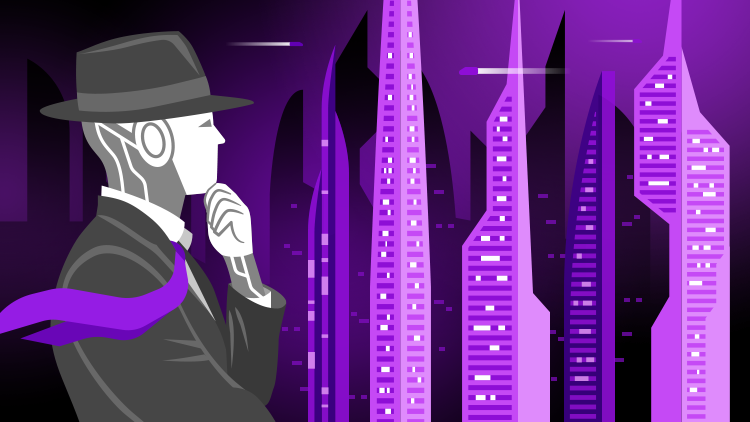
\includegraphics[scale=0.6]{Course_Image.png}
		\end{center}
\end{figure}

\end{titlepage}

{
\setcounter{tocdepth}{1}
\tableofcontents
}
\textbackslash{}begin\{titlepage\}

\setcounter{tocdepth}{4}
\renewcommand{\contentsname}{Tabla de Contenidos}
\tableofcontents

\newpage

\hypertarget{introducciuxf3n}{%
\chapter*{Introducción}\label{introducciuxf3n}}
\addcontentsline{toc}{chapter}{Introducción}

Este libro es el complemento de nuestro curso online \emph{Inteligencia Artificial aplicada a Negocios y Empresas} disponible en \href{https://www.udemy.com/ia4business/?couponCode=THEBOOK}{Udemy}. Cubre los tres casos prácticos de empresa reales que se resuelven, cada uno de ellos, con una técnica diferente del mundo de la inteligencia artificial:

\begin{longtable}[]{@{}ccc@{}}
\toprule
\begin{minipage}[b]{0.19\columnwidth}\centering
\textbf{Part}\strut
\end{minipage} & \begin{minipage}[b]{0.34\columnwidth}\centering
\textbf{Case Study}\strut
\end{minipage} & \begin{minipage}[b]{0.38\columnwidth}\centering
\textbf{AI Solution}\strut
\end{minipage}\tabularnewline
\midrule
\endhead
\begin{minipage}[t]{0.19\columnwidth}\centering
1 - Optimización de Procesos\strut
\end{minipage} & \begin{minipage}[t]{0.34\columnwidth}\centering
Optimizar el flujo en los almacenes de un ecommerce\strut
\end{minipage} & \begin{minipage}[t]{0.38\columnwidth}\centering
Q-Learning\strut
\end{minipage}\tabularnewline
\begin{minipage}[t]{0.19\columnwidth}\centering
2 - Minimización de Costes\strut
\end{minipage} & \begin{minipage}[t]{0.34\columnwidth}\centering
Minimizar los gastos de energía del servidor de un centro de datos\strut
\end{minipage} & \begin{minipage}[t]{0.38\columnwidth}\centering
Deep Q-Learning\strut
\end{minipage}\tabularnewline
\begin{minipage}[t]{0.19\columnwidth}\centering
3 - Maximización de Beneficios\strut
\end{minipage} & \begin{minipage}[t]{0.34\columnwidth}\centering
Mazimizar los beneficios de un negocio online de venta al por menor\strut
\end{minipage} & \begin{minipage}[t]{0.38\columnwidth}\centering
Muestreo Thompson\strut
\end{minipage}\tabularnewline
\bottomrule
\end{longtable}

En cada una de esas partes, seguiremos el mismo esquema de tres pasos:

\begin{itemize}
\tightlist
\item
  \textbf{Caso Práctico} Comenzaremos explicando el problema que tenemos que resolver y construiremos desde cero el entorno en el que trabajaremos.
\item
  \textbf{AI Solution.} Te daremos no solo la teoría general sino también todos los detalles matemáticos del modelo de IA que resolverán el caso práctico
\item
  \textbf{Implementation.} Implementaremos toda la solución de inteligencia artificial en Python, lo pondremos en producción y mejoraremos la inteligencia artificial al completar tareas adicionales al final.
\end{itemize}

¡Muchas gracias a todos por unirte a nosotros en este curso, te deseo sin duda un emocionante viaje al mundo de la IA aplicada a Negocios y Empresas con nosotros!

\hypertarget{optimizaciuxf3n-de-procesos}{%
\chapter{Optimización de Procesos}\label{optimizaciuxf3n-de-procesos}}

Aquí vamos con nuestro primer caso práctico y nuestro primer modelo de IA. ¡Esperamos que estés listo!

\hypertarget{caso-pruxe1ctico-optimizaciuxf3n-de-tareas-en-un-almacuxe9n-de-comercio-electruxf3nico}{%
\section{Caso Práctico: Optimización de tareas en un almacén de comercio electrónico}\label{caso-pruxe1ctico-optimizaciuxf3n-de-tareas-en-un-almacuxe9n-de-comercio-electruxf3nico}}

\hypertarget{problema-a-resolver}{%
\subsection{Problema a resolver}\label{problema-a-resolver}}

El problema a resolver será optimizar los flujos dentro del siguiente almacén:

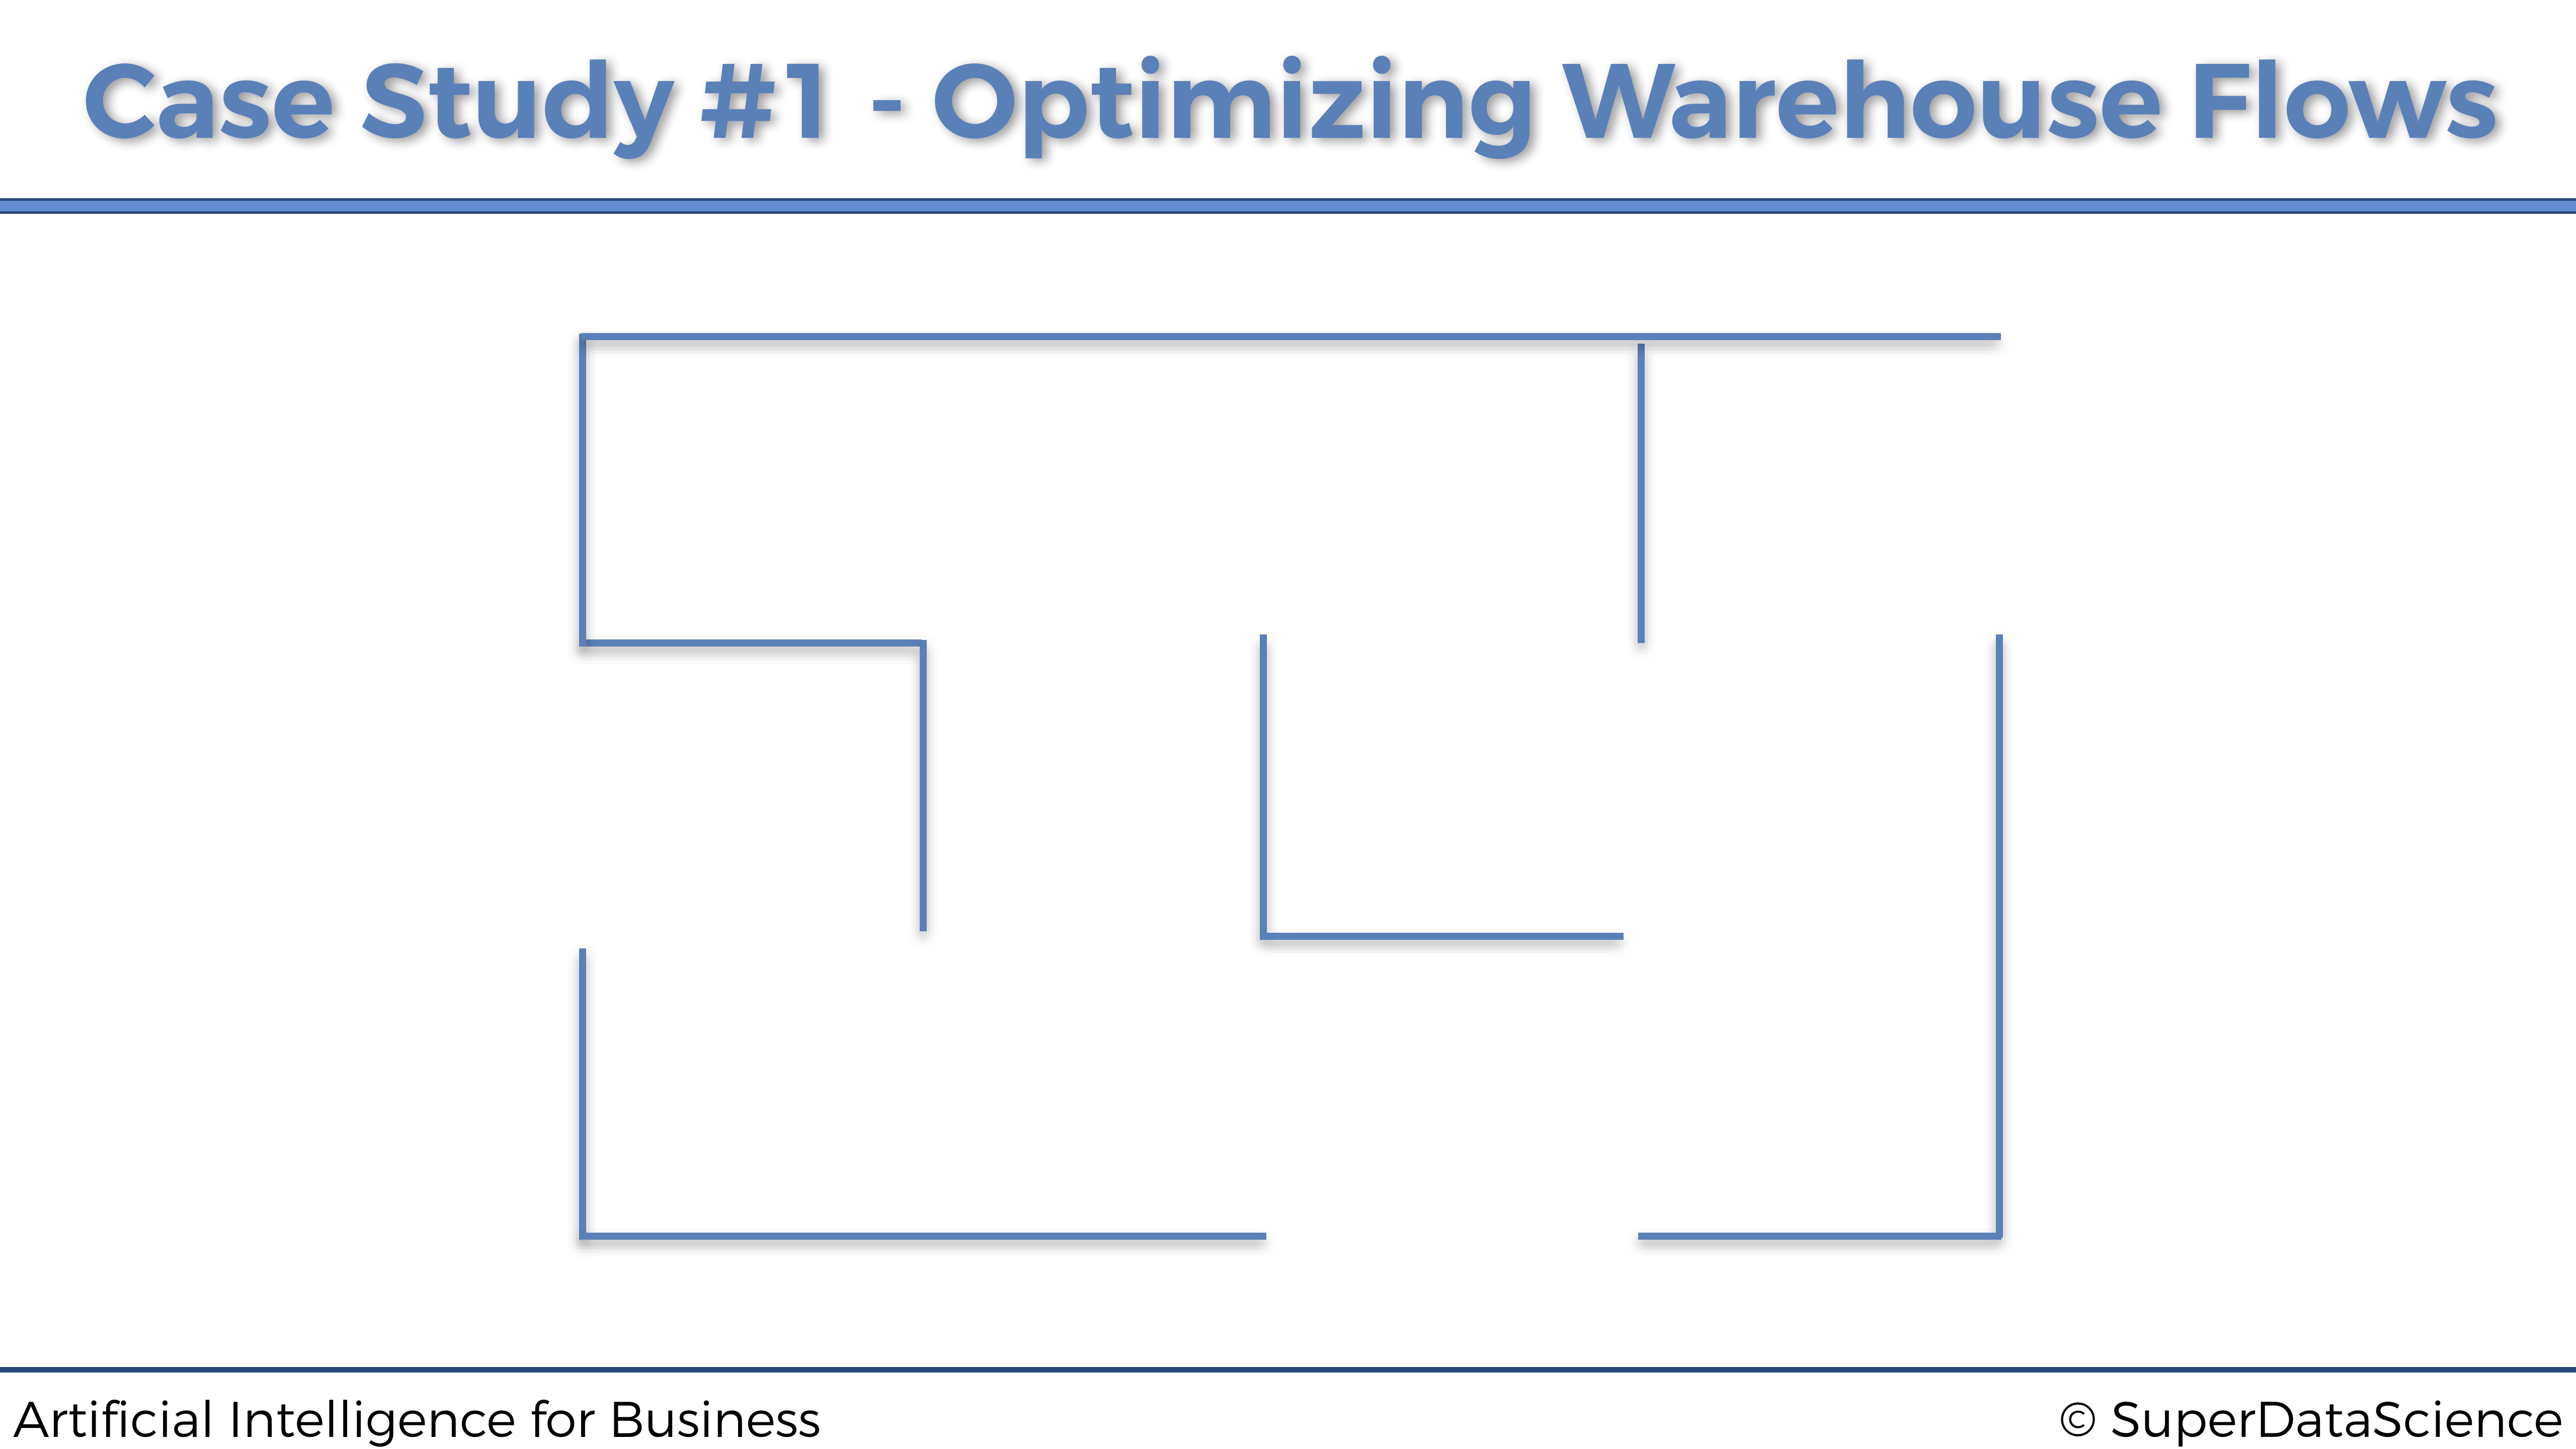
\includegraphics[width=1\textwidth,height=\textheight]{Images/Warehouse_1.png}

El almacén pertenece a una empresa online minorista que vende productos a una variedad de clientes. Dentro de este almacén, los productos se almacenan en 12 ubicaciones diferentes, etiquetadas con las siguientes letras de la A a la L:

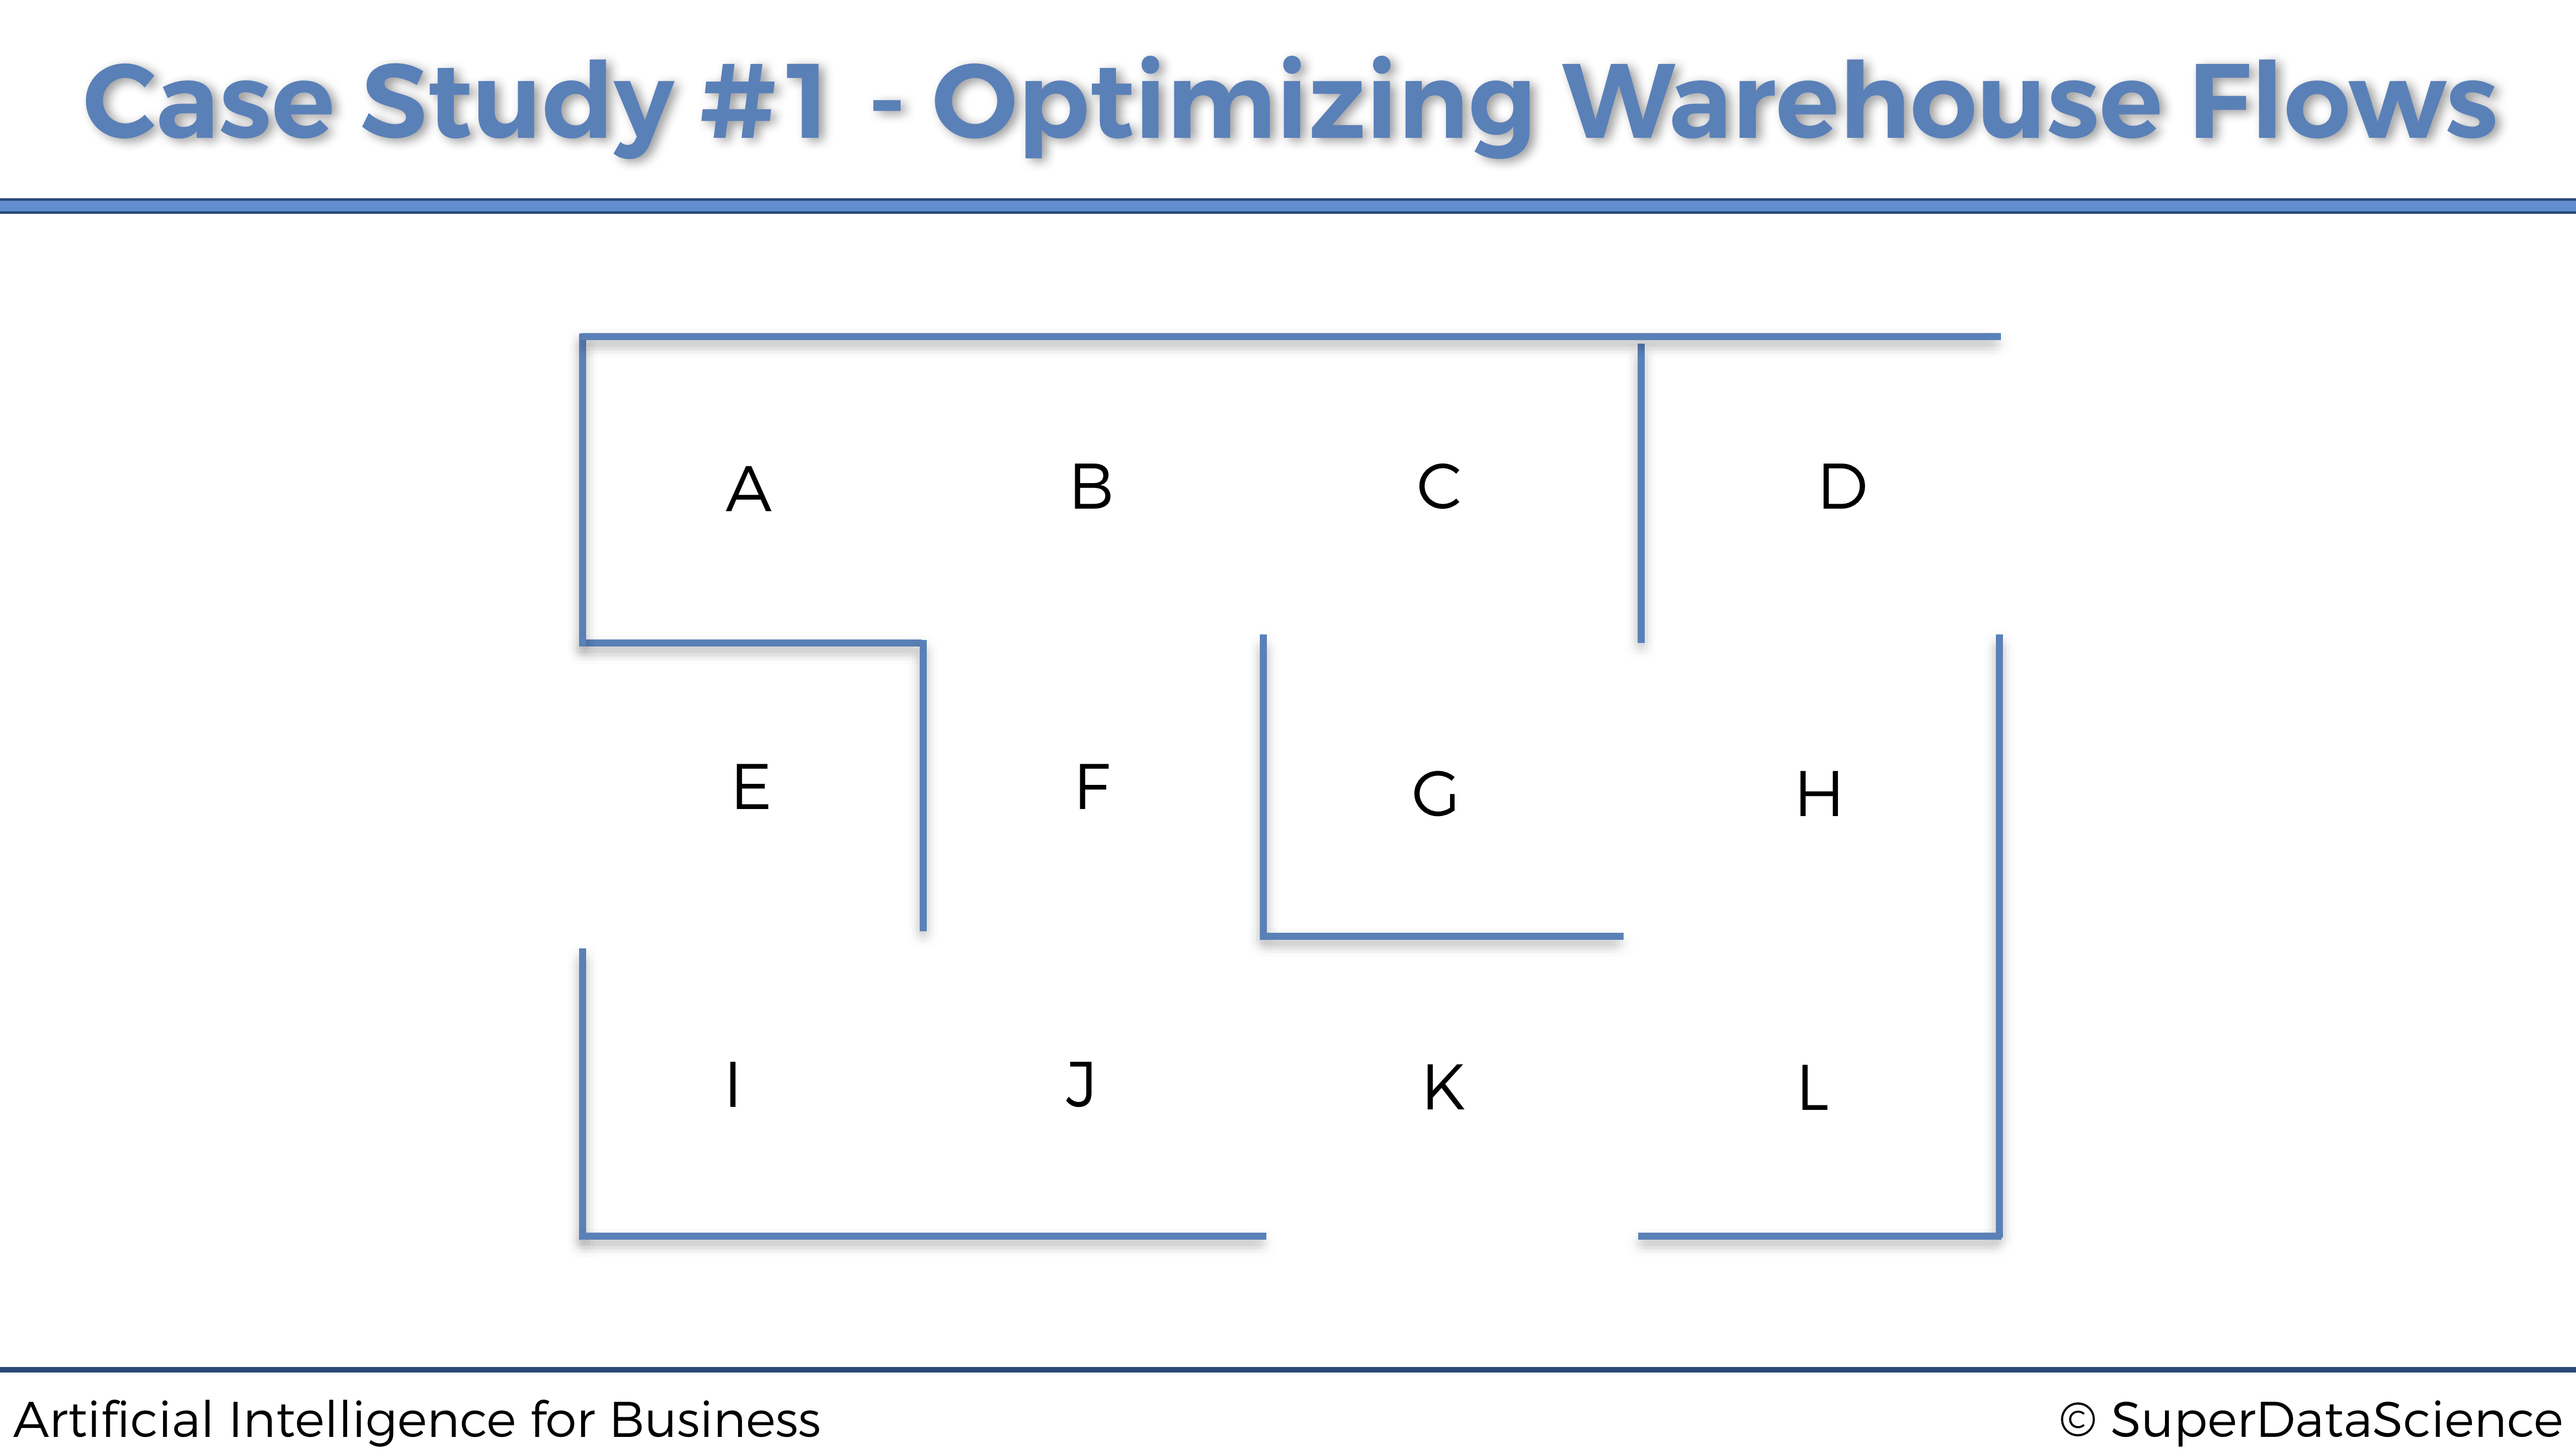
\includegraphics[width=1\textwidth,height=\textheight]{Images/Warehouse_2.png}

A medida que los clientes hacen los pedidos online, un robot de almacén autónomo se mueve por el almacén para recoger los productos para futuras entregas. Así es como se ve:

\begin{figure}
\centering
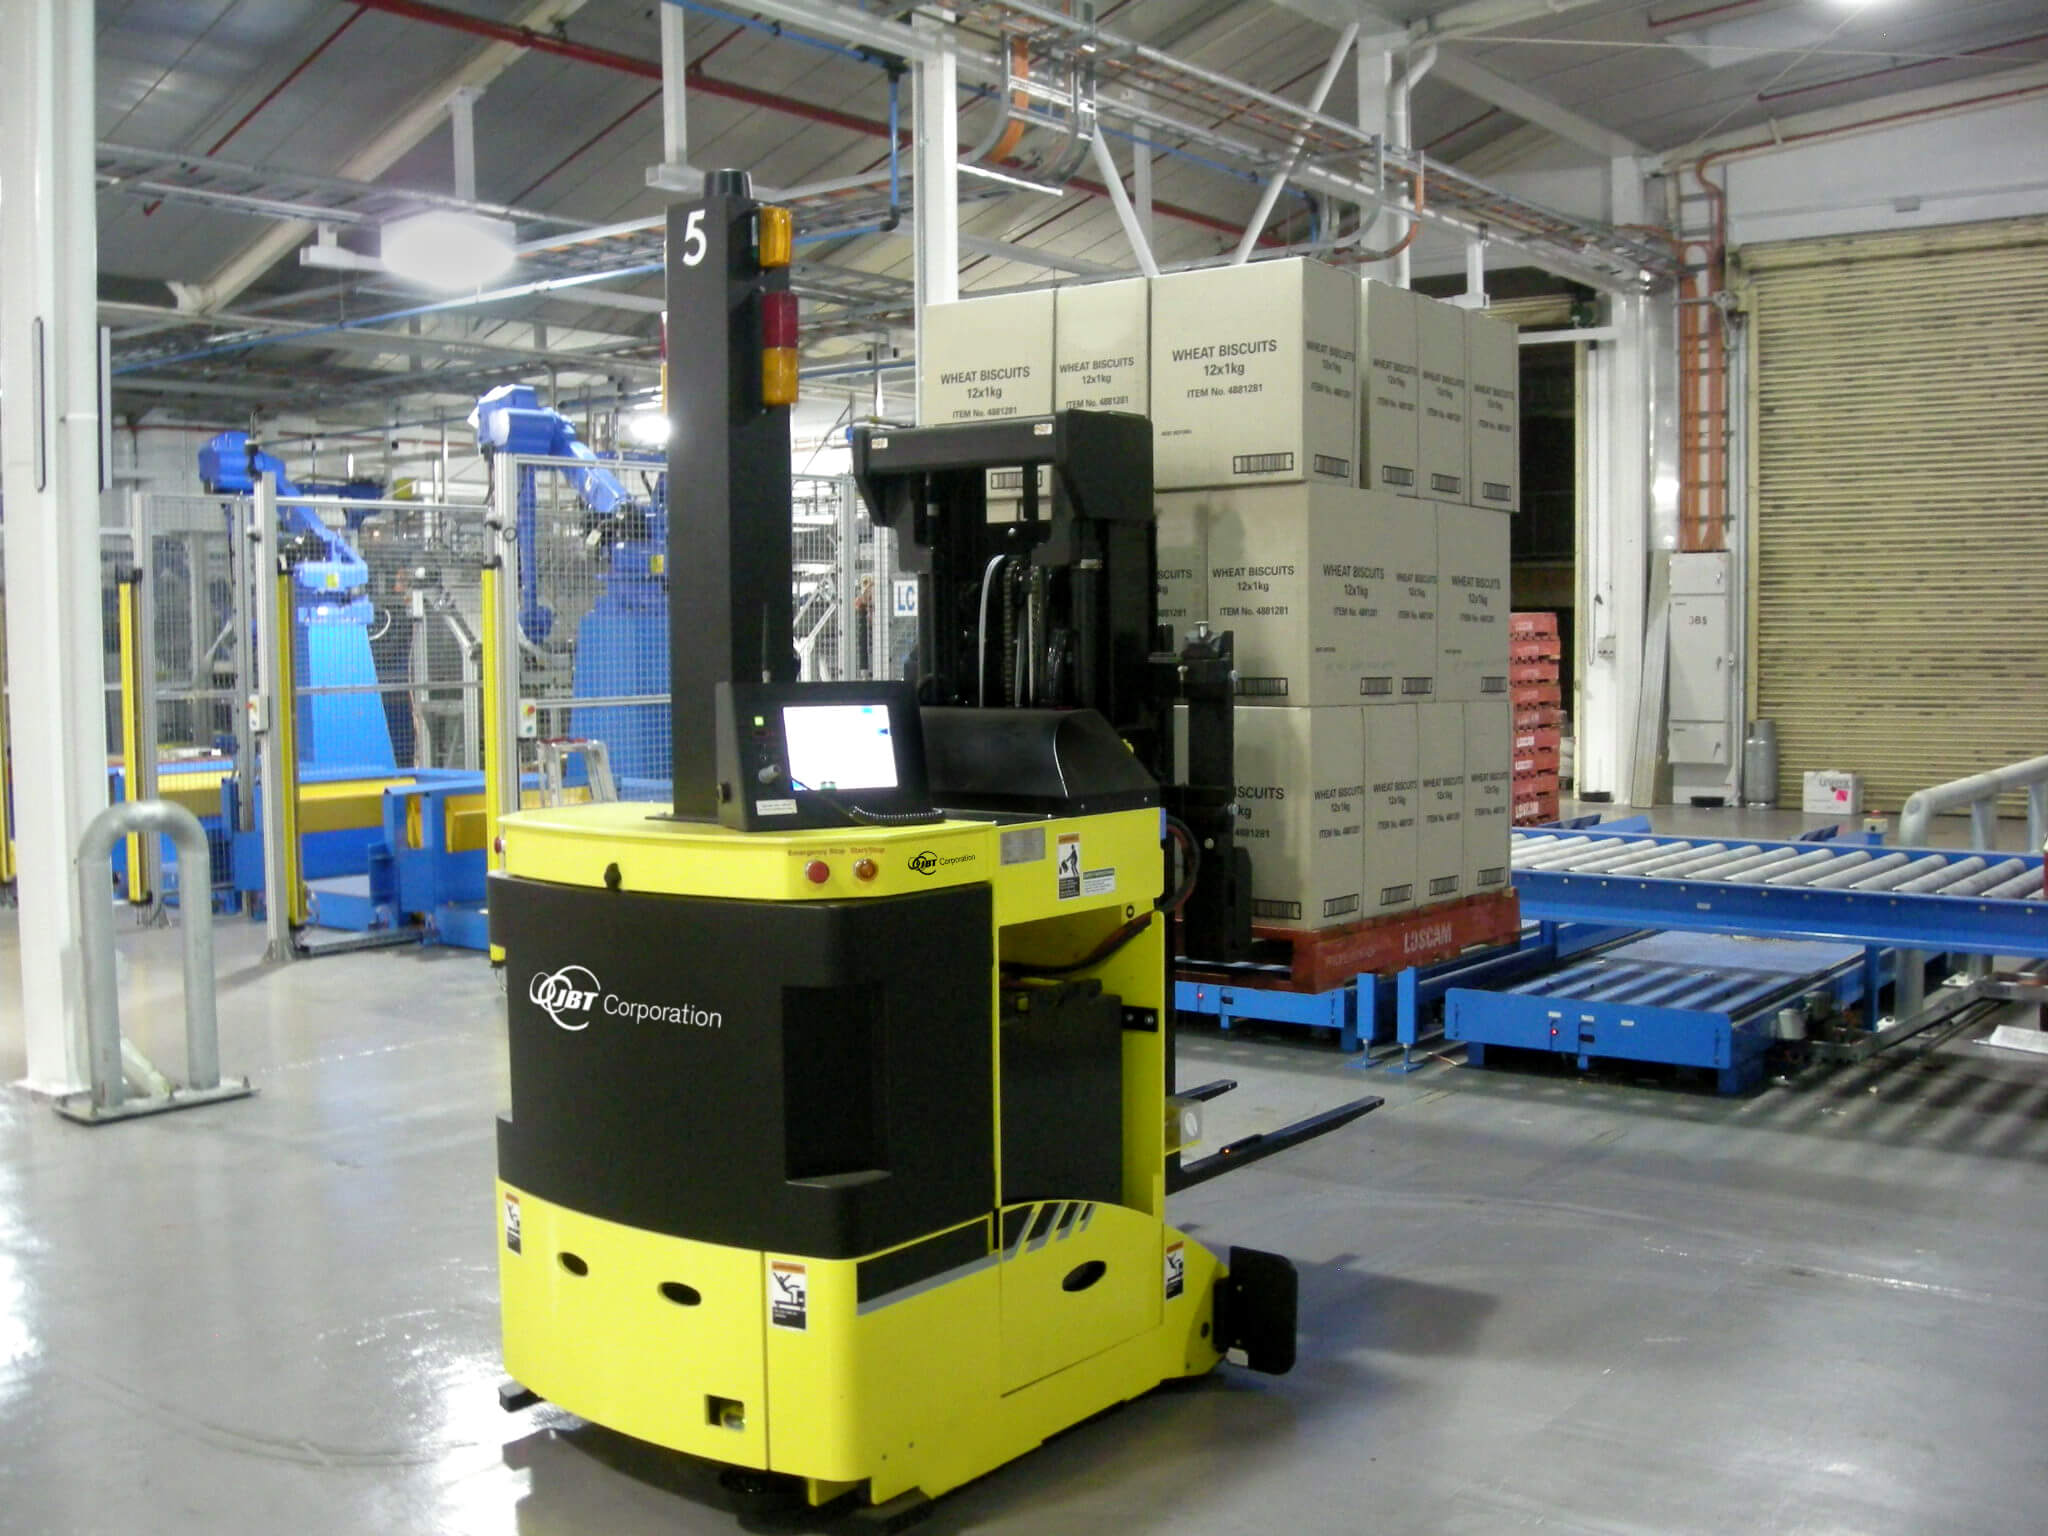
\includegraphics[width=1\textwidth,height=\textheight]{Images/Autonomous_Warehouse_Robot.jpg}
\caption{Autonomous Warehouse Robot}
\end{figure}

Las 12 ubicaciones están conectadas a un sistema informático, que clasifica en tiempo real las prioridades de recolección de productos para estas 12 ubicaciones. Por ejemplo, en un momento específico \(t\), devolverá la siguiente clasificación:

\begin{longtable}[]{@{}cc@{}}
\toprule
\textbf{Rango de Prioridad} & \textbf{Ubicación}\tabularnewline
\midrule
\endhead
1 & G\tabularnewline
2 & K\tabularnewline
3 & L\tabularnewline
4 & J\tabularnewline
5 & A\tabularnewline
6 & I\tabularnewline
7 & H\tabularnewline
8 & C\tabularnewline
9 & B\tabularnewline
10 & D\tabularnewline
11 & F\tabularnewline
12 & E\tabularnewline
\bottomrule
\end{longtable}

La ubicación G tiene prioridad 1, lo que significa que es la máxima prioridad, ya que contiene un producto que debe recogerse y entregarse de inmediato. Nuestro robot de almacén autónomo debe moverse a la ubicación G por la ruta más corta, dependiendo de dónde se encuentre. Nuestro objetivo es construir una IA que regrese esa ruta más corta, donde sea que esté el robot. Pero luego, como vemos, las ubicaciones K y L están en las 3 prioridades principales. Por lo tanto, querremos implementar una opción para que nuestro Robot de almacén autónomo pase por algunas ubicaciones intermedias antes de llegar a su ubicación final de máxima prioridad.

La forma en que el sistema calcula las prioridades de las ubicaciones está fuera del alcance de este caso práctico. La razón de esto es que puede haber muchas formas, desde reglas o algoritmos simples, hasta cálculos deterministas y aprendizaje automático. Pero la mayoría de estas formas no serían inteligencia artificial como la conocemos hoy. En lo que realmente queremos centrarnos es en la IA central, que abarca Q-Learning, Deep Q-Learning y otras ramas de Reinforcement Learning. Entonces, solo diremos, por ejemplo, que la ubicación G es la máxima prioridad porque uno de los clientes de platino más leales de la compañía hizo un pedido urgente de un producto almacenado en la ubicación G, que por lo tanto debe entregarse lo antes posible.

Por lo tanto, en conclusión, nuestra misión es construir una IA que siempre tome la ruta más corta a la ubicación de máxima prioridad, sea cual sea la ubicación desde la que comienza, y tener la opción de ir a una ubicación intermedia que se encuentre entre las 3 prioridades principales.

\hypertarget{entorno-a-definir}{%
\subsection{Entorno a definir}\label{entorno-a-definir}}

Al construir una IA, lo primero que siempre tenemos que hacer es definir el entorno. Y definir un entorno siempre requiere los tres elementos siguientes:

\begin{itemize}
\tightlist
\item
  Definir los estados
\item
  Definir las acciones
\item
  Definir las recompensas
\end{itemize}

Definamos estos tres elementos, uno por uno.

\textbf{Definir los estados.}

Comencemos con los estados. El estado de entrada es simplemente la ubicación donde está nuestro Robot de almacén autónomo en cada momento \(t\). Sin embargo, dado que construiremos nuestra IA con ecuaciones matemáticas, codificaremos los nombres de las ubicaciones (A, B, C, \ldots{}) en números de índice, con respecto a la siguiente asignación:

\begin{longtable}[]{@{}cc@{}}
\toprule
\textbf{Ubicación} & \textbf{Estado}\tabularnewline
\midrule
\endhead
A & 0\tabularnewline
B & 1\tabularnewline
C & 2\tabularnewline
D & 3\tabularnewline
E & 4\tabularnewline
F & 5\tabularnewline
G & 6\tabularnewline
H & 7\tabularnewline
I & 8\tabularnewline
J & 9\tabularnewline
K & 10\tabularnewline
L & 11\tabularnewline
\bottomrule
\end{longtable}

Hay una razón específica por la que codificamos los estados con índices del 0 al 11, en lugar de otros enteros. La razón es que trabajaremos con matrices, una matriz de recompensas y una matriz de valores Q, y cada línea y columna de estas matrices corresponderá a una ubicación específica. Por ejemplo, la primera línea de cada matriz, que tiene el índice 0, corresponde a la ubicación A. La segunda línea / columna, que tiene el índice 1, corresponde a la ubicación B. Etc. Veremos el propósito de trabajar con matrices con más detalles. un poco más tarde.

\textbf{Definir las acciones.}

Ahora definamos las posibles acciones a realizar Las acciones son simplemente los siguientes movimientos que el robot puede hacer para ir de un lugar a otro. Entonces, por ejemplo, digamos que el robot está en la ubicación J, las posibles acciones que el robot puede llevar a cabo es ir a I, F o K. Y nuevamente, ya que trabajaremos con ecuaciones matemáticas, codificaremos estas acciones con los mismos índices que para los estados. Por lo tanto, siguiendo nuestro mismo ejemplo donde el robot está en la ubicación J en un momento específico, las posibles acciones que el robot puede jugar son, de acuerdo con nuestro mapeo anterior anterior: 5, 8 y 10. De hecho, el índice 5 corresponde a F, el índice 8 corresponde a I y el índice 10 corresponde a K. Por lo tanto, eventualmente, la lista total de acciones que la IA puede llevar a cabo en general es la siguiente:

\[actions = [0,1,2,3,4,5,6,7,8,9,10,11]\]

Obviamente, al estar en una ubicación específica, hay algunas acciones que el robot no puede llevar a cabo. Tomando el mismo ejemplo anterior, si el robot está en la ubicación J, puede ejecutar las acciones 5, 8 y 10, pero no puede ejecutar las otras acciones. Nos aseguraremos de especificar eso al atribuir una recompensa 0 a las acciones que no puede llevar a cabo, y una recompensa 1 a las acciones que si puede realizar. Y eso nos lleva a las recompensas.

\textbf{Definir las recompensas.}

Lo último que tenemos que hacer ahora para construir nuestro entorno es definir un sistema de recompensas. Más específicamente, tenemos que definir una función de recompensa \(R\) que toma como entradas un estado \(s\) y una acción \(a\), y devuelve una recompensa numérica que la IA obtendrá al llevar a cabo la acción \(a\) en el estado \(s\):

\[R : (\textrm{state}, \textrm{action}) \mapsto r \in \mathbb{R}\]

Entonces, ¿cómo vamos a construir esa función para nuestro caso práctico? Aquí esto es simple. Dado que hay un número discreto y finito de estados (los índices de 0 a 11), así como un número discreto y finito de acciones (mismos índices de 0 a 11), la mejor manera de construir nuestra función de recompensa R es simplemente hacer una matriz. Nuestra función de recompensa será exactamente una matriz de 12 filas y 12 columnas, donde las filas corresponden a los estados y las columnas corresponden a las acciones. De esa forma, en nuestra función \$R: (s, a) \mapsto r ~in \mathbb{R} \$, \(s\) será el índice de la fila de la matriz, \(a\) será el índice de la columna de matriz, y \(r\) será la celda de los índices \((s, a)\) en la matriz.

Por lo tanto, lo único que tenemos que hacer ahora para definir nuestra función de recompensa es simplemente llenar esta matriz con las recompensas numéricas. Y como acabamos de decir en el párrafo anterior, lo que tenemos que hacer primero es atribuir, para cada una de las 12 ubicaciones, una recompensa 0 por las acciones que el robot no puede ejecutar, y una recompensa 1 por las acciones que el robot puede llevar a cabo. Al hacer eso para cada una de las 12 ubicaciones, terminaremos con una matriz de recompensas. Vamos a construirlo paso a paso, comenzando con la primera ubicación:

\emph{Ubicación A.}

Cuando se encuentra en la ubicación A, el robot solo puede ir a la ubicación B. Por lo tanto, dado que la ubicación A tiene el índice 0 (primera fila de la matriz) y la ubicación B tiene el índice 1 (segunda columna de la matriz), la primera fila de la matriz de las recompensas obtendrá un 1 en la segunda columna y un 0 en todas las otras columnas, así:

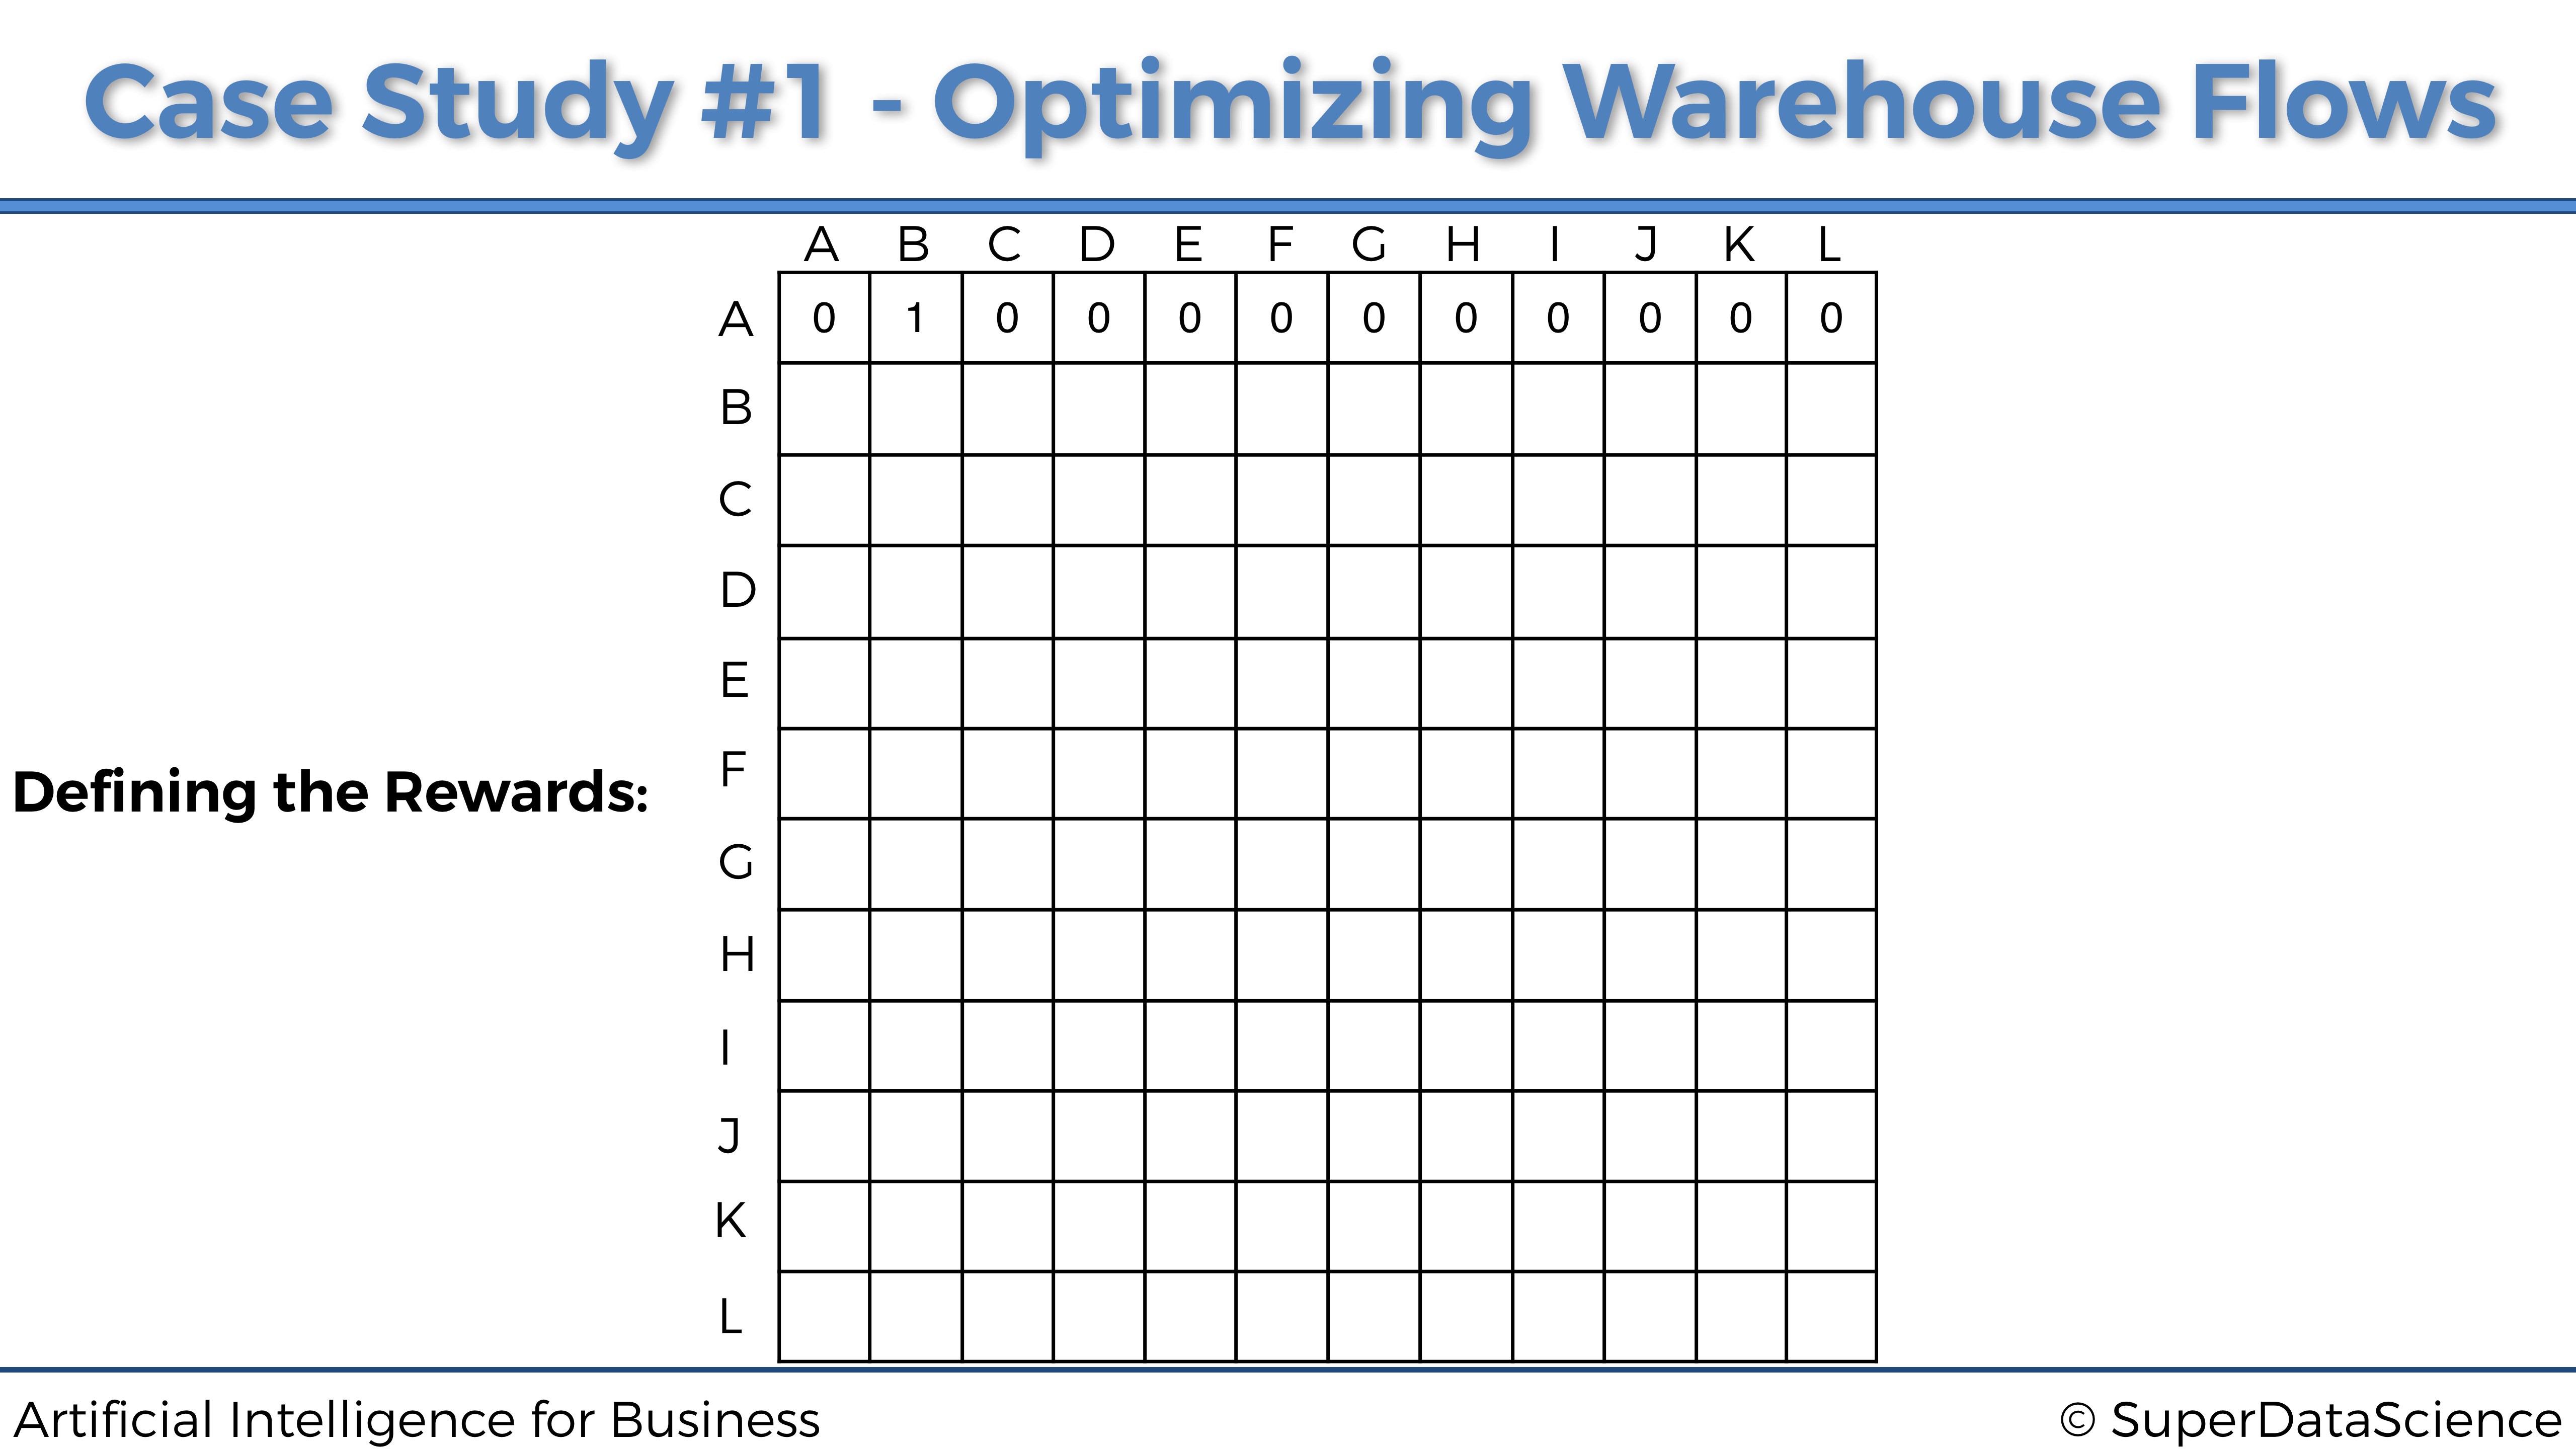
\includegraphics{Images/Rewards_Matrix_1.png}

\emph{Ubicación B.}

Al estar en la ubicación B, el robot solo puede ir a tres ubicaciones diferentes: A, C y F. Dado que B tiene el índice 1 (segunda fila), y A, C, F tienen los índices respectivos 0, 2, 5 (1ra, 3ra. , y sexta columna), entonces la segunda fila de la matriz de recompensas obtendrá un 1 en las columnas 1a, 3a y 6a, y 0 en todas las otras columnas. Por lo tanto obtenemos:

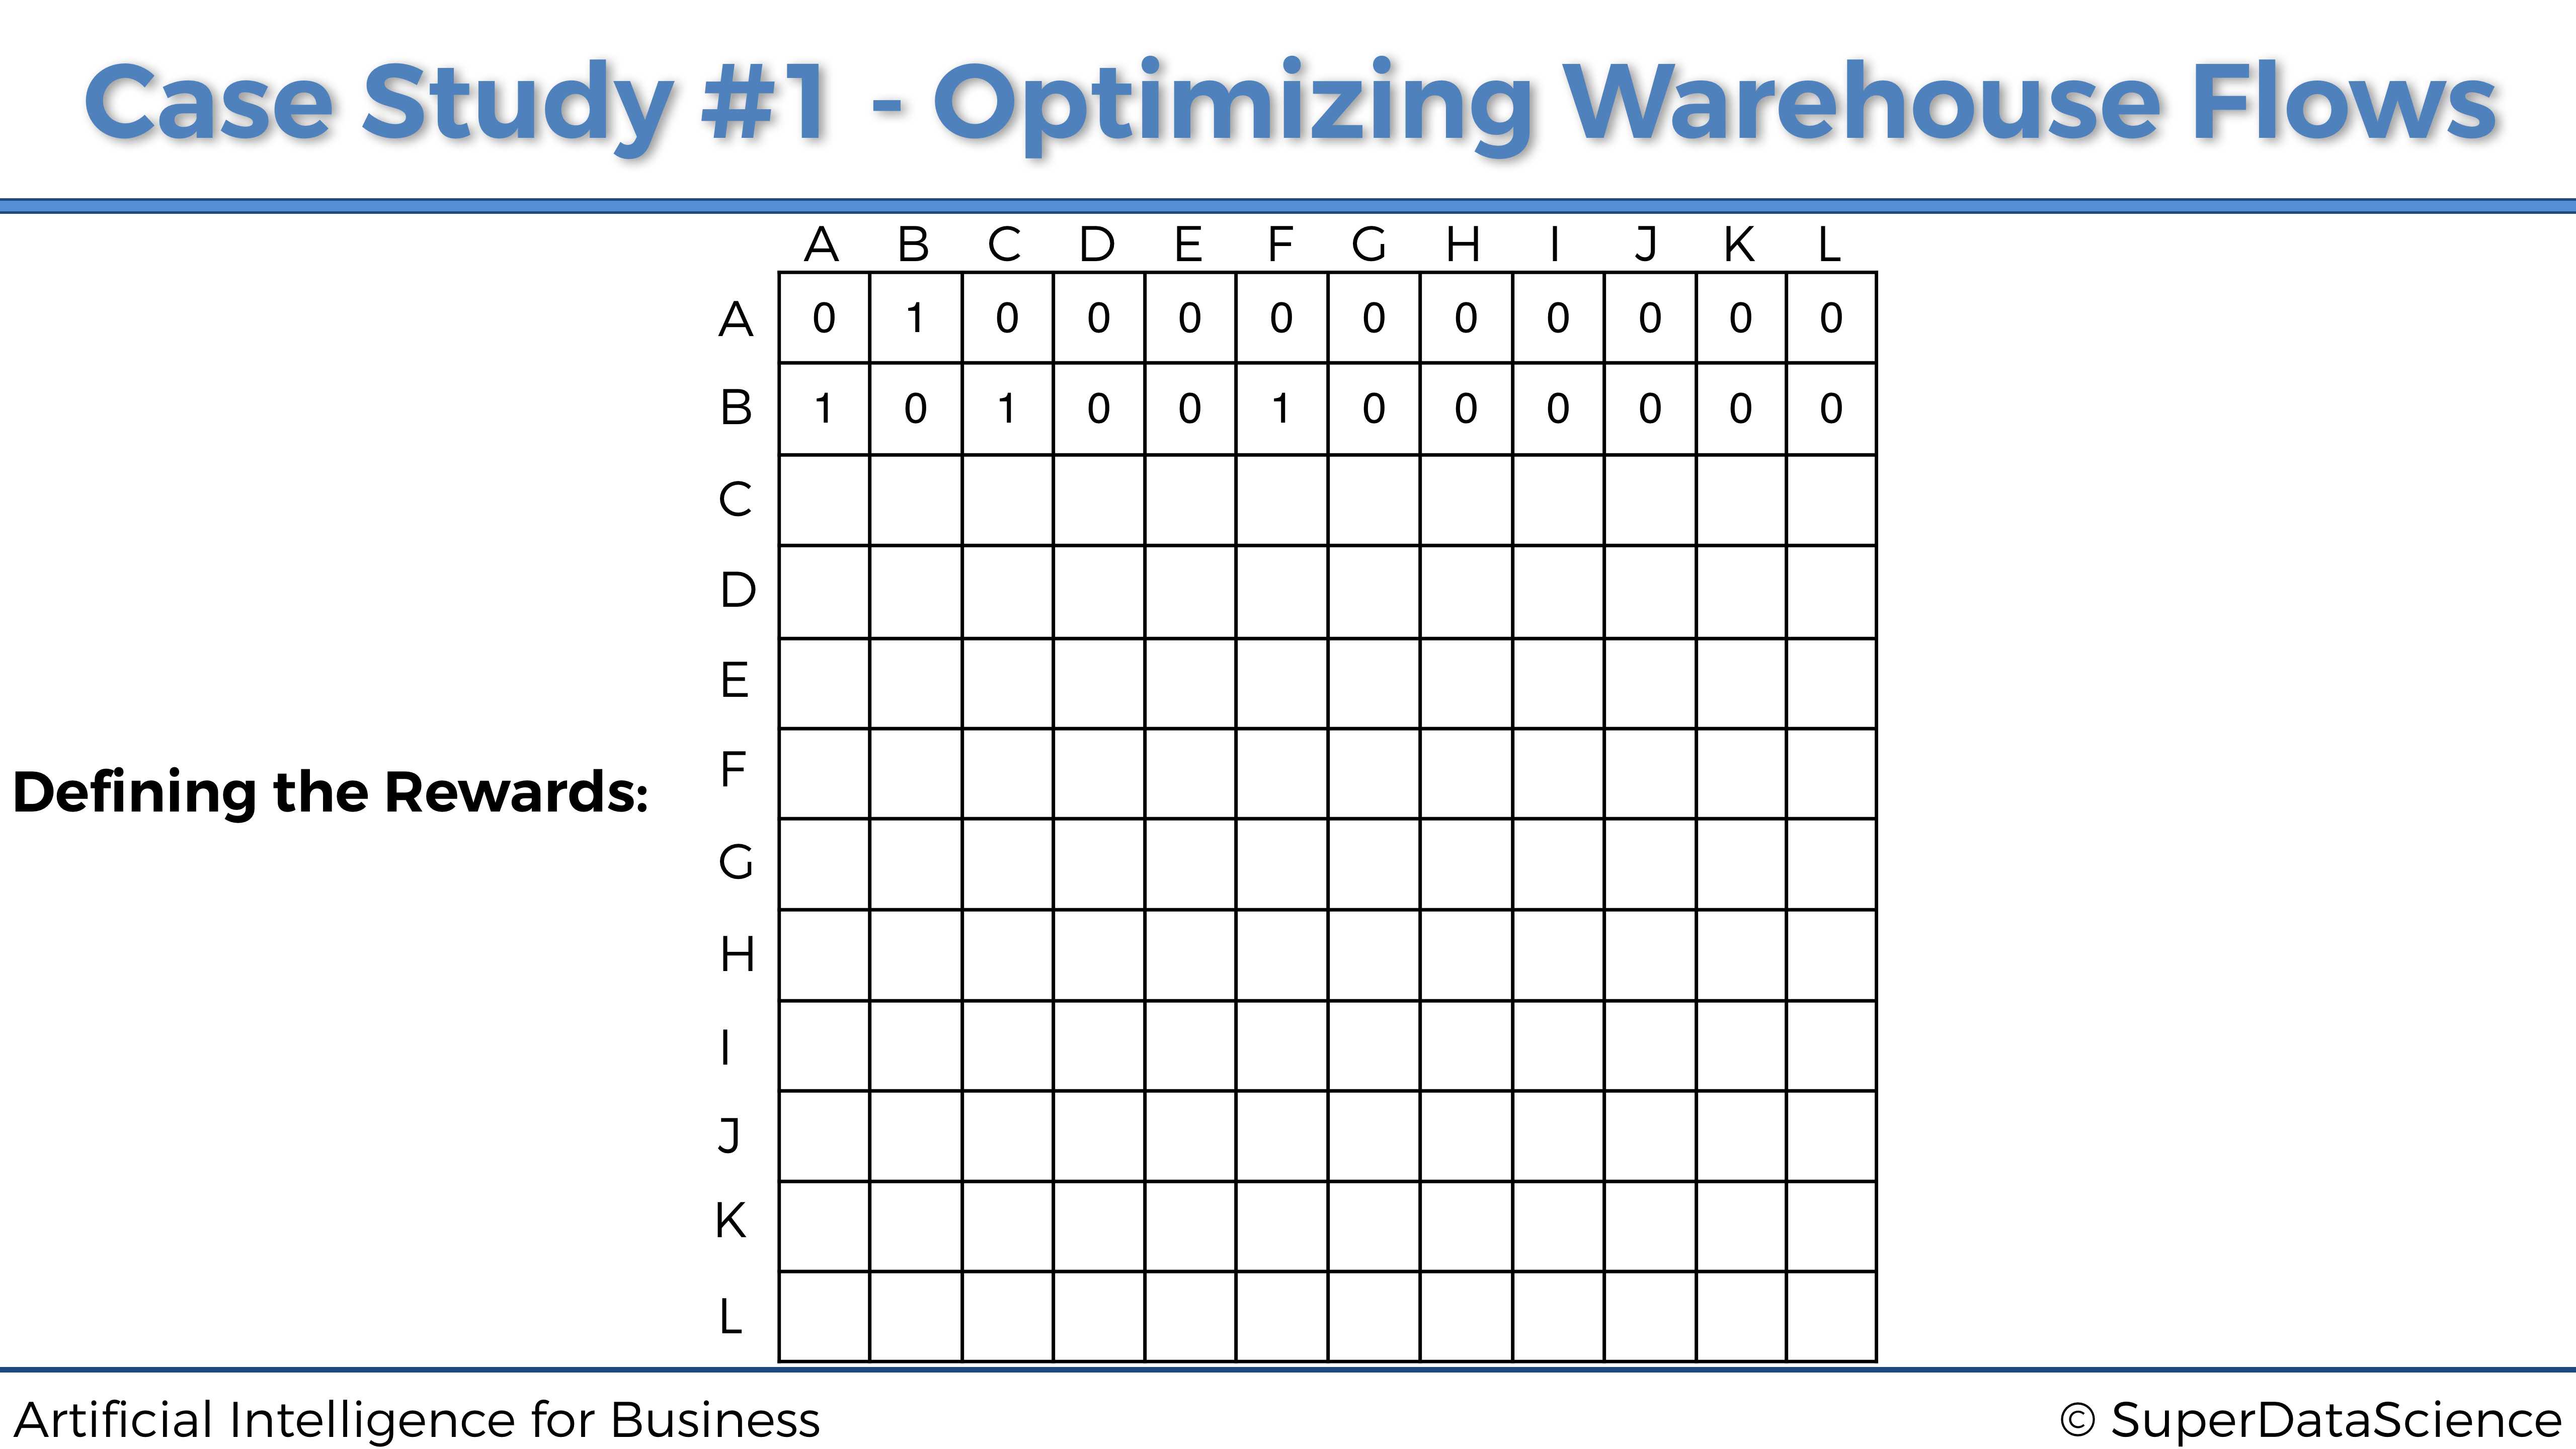
\includegraphics{Images/Rewards_Matrix_2.png}

\emph{Ubicación C.}

Ocurre lo mismo, la ubicación C (de índice 2) solo está conectada a B y G (de índices 1 y 6), por lo que la tercera fila de la matriz de recompensas es:

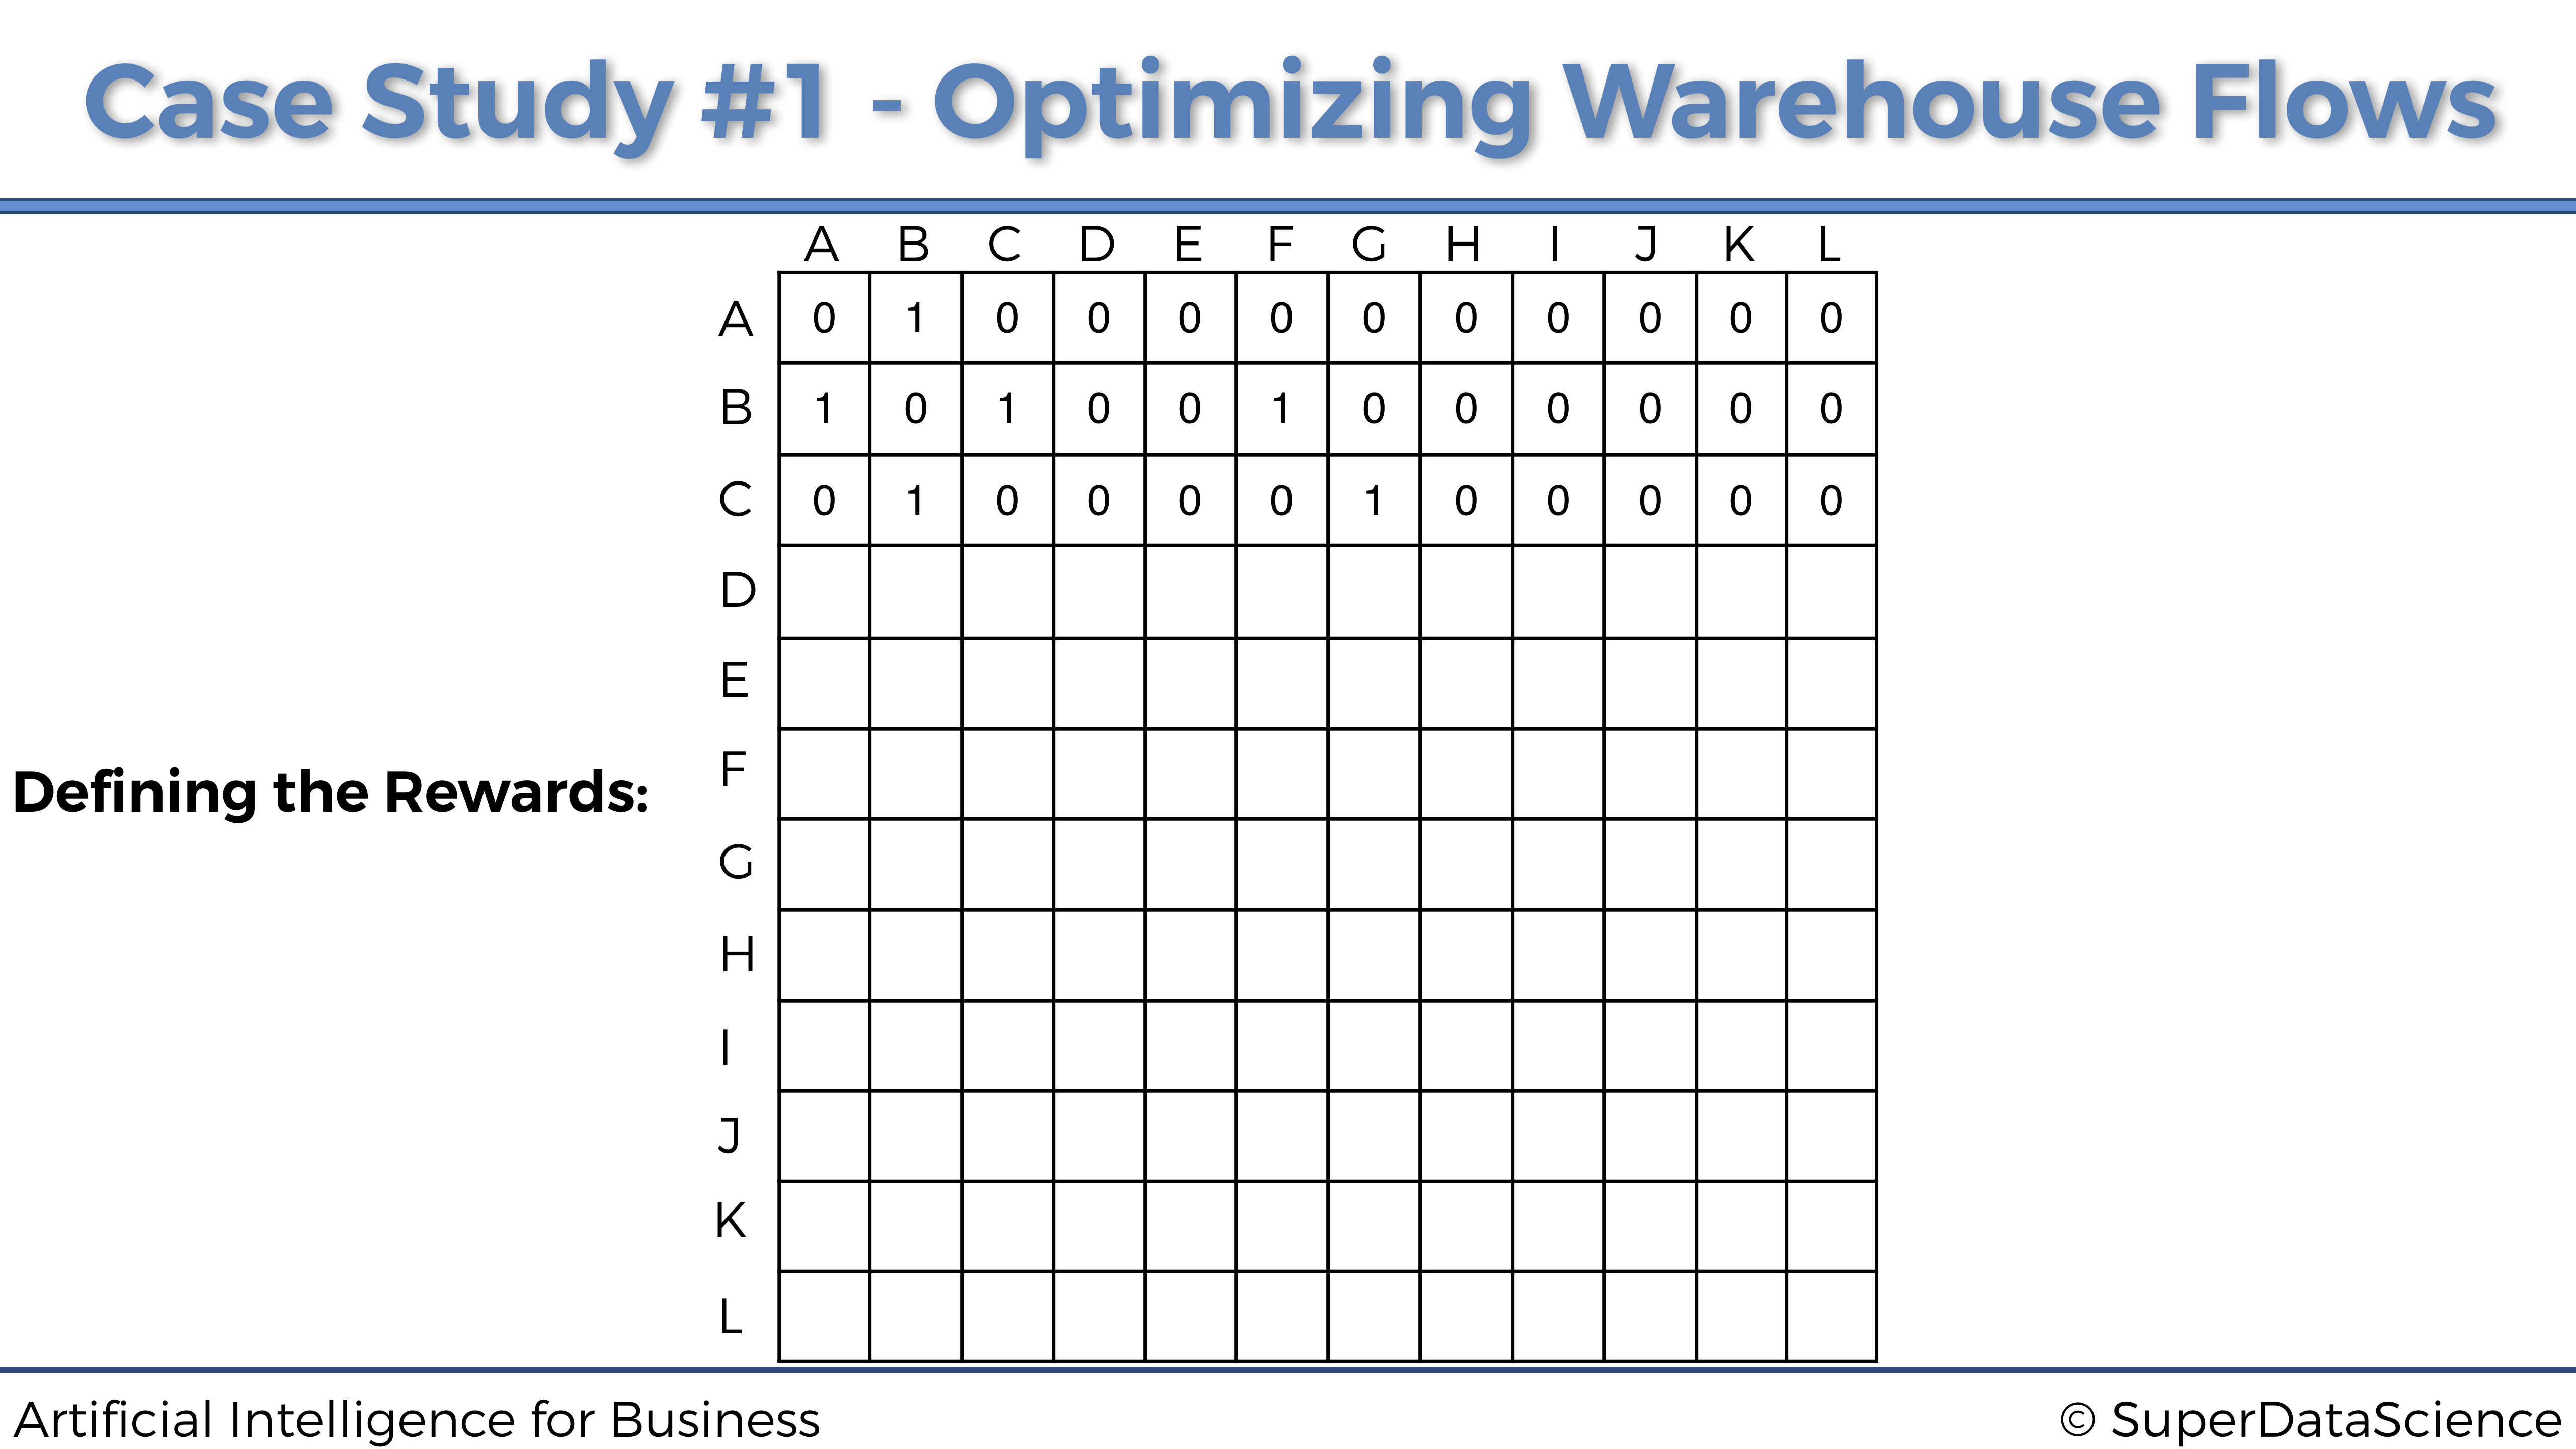
\includegraphics{Images/Rewards_Matrix_3.png}

\emph{En el resto de ubicaciones\ldots{}}

Al hacer lo mismo para todas las demás ubicaciones, finalmente obtenemos nuestra matriz final de recompensas:

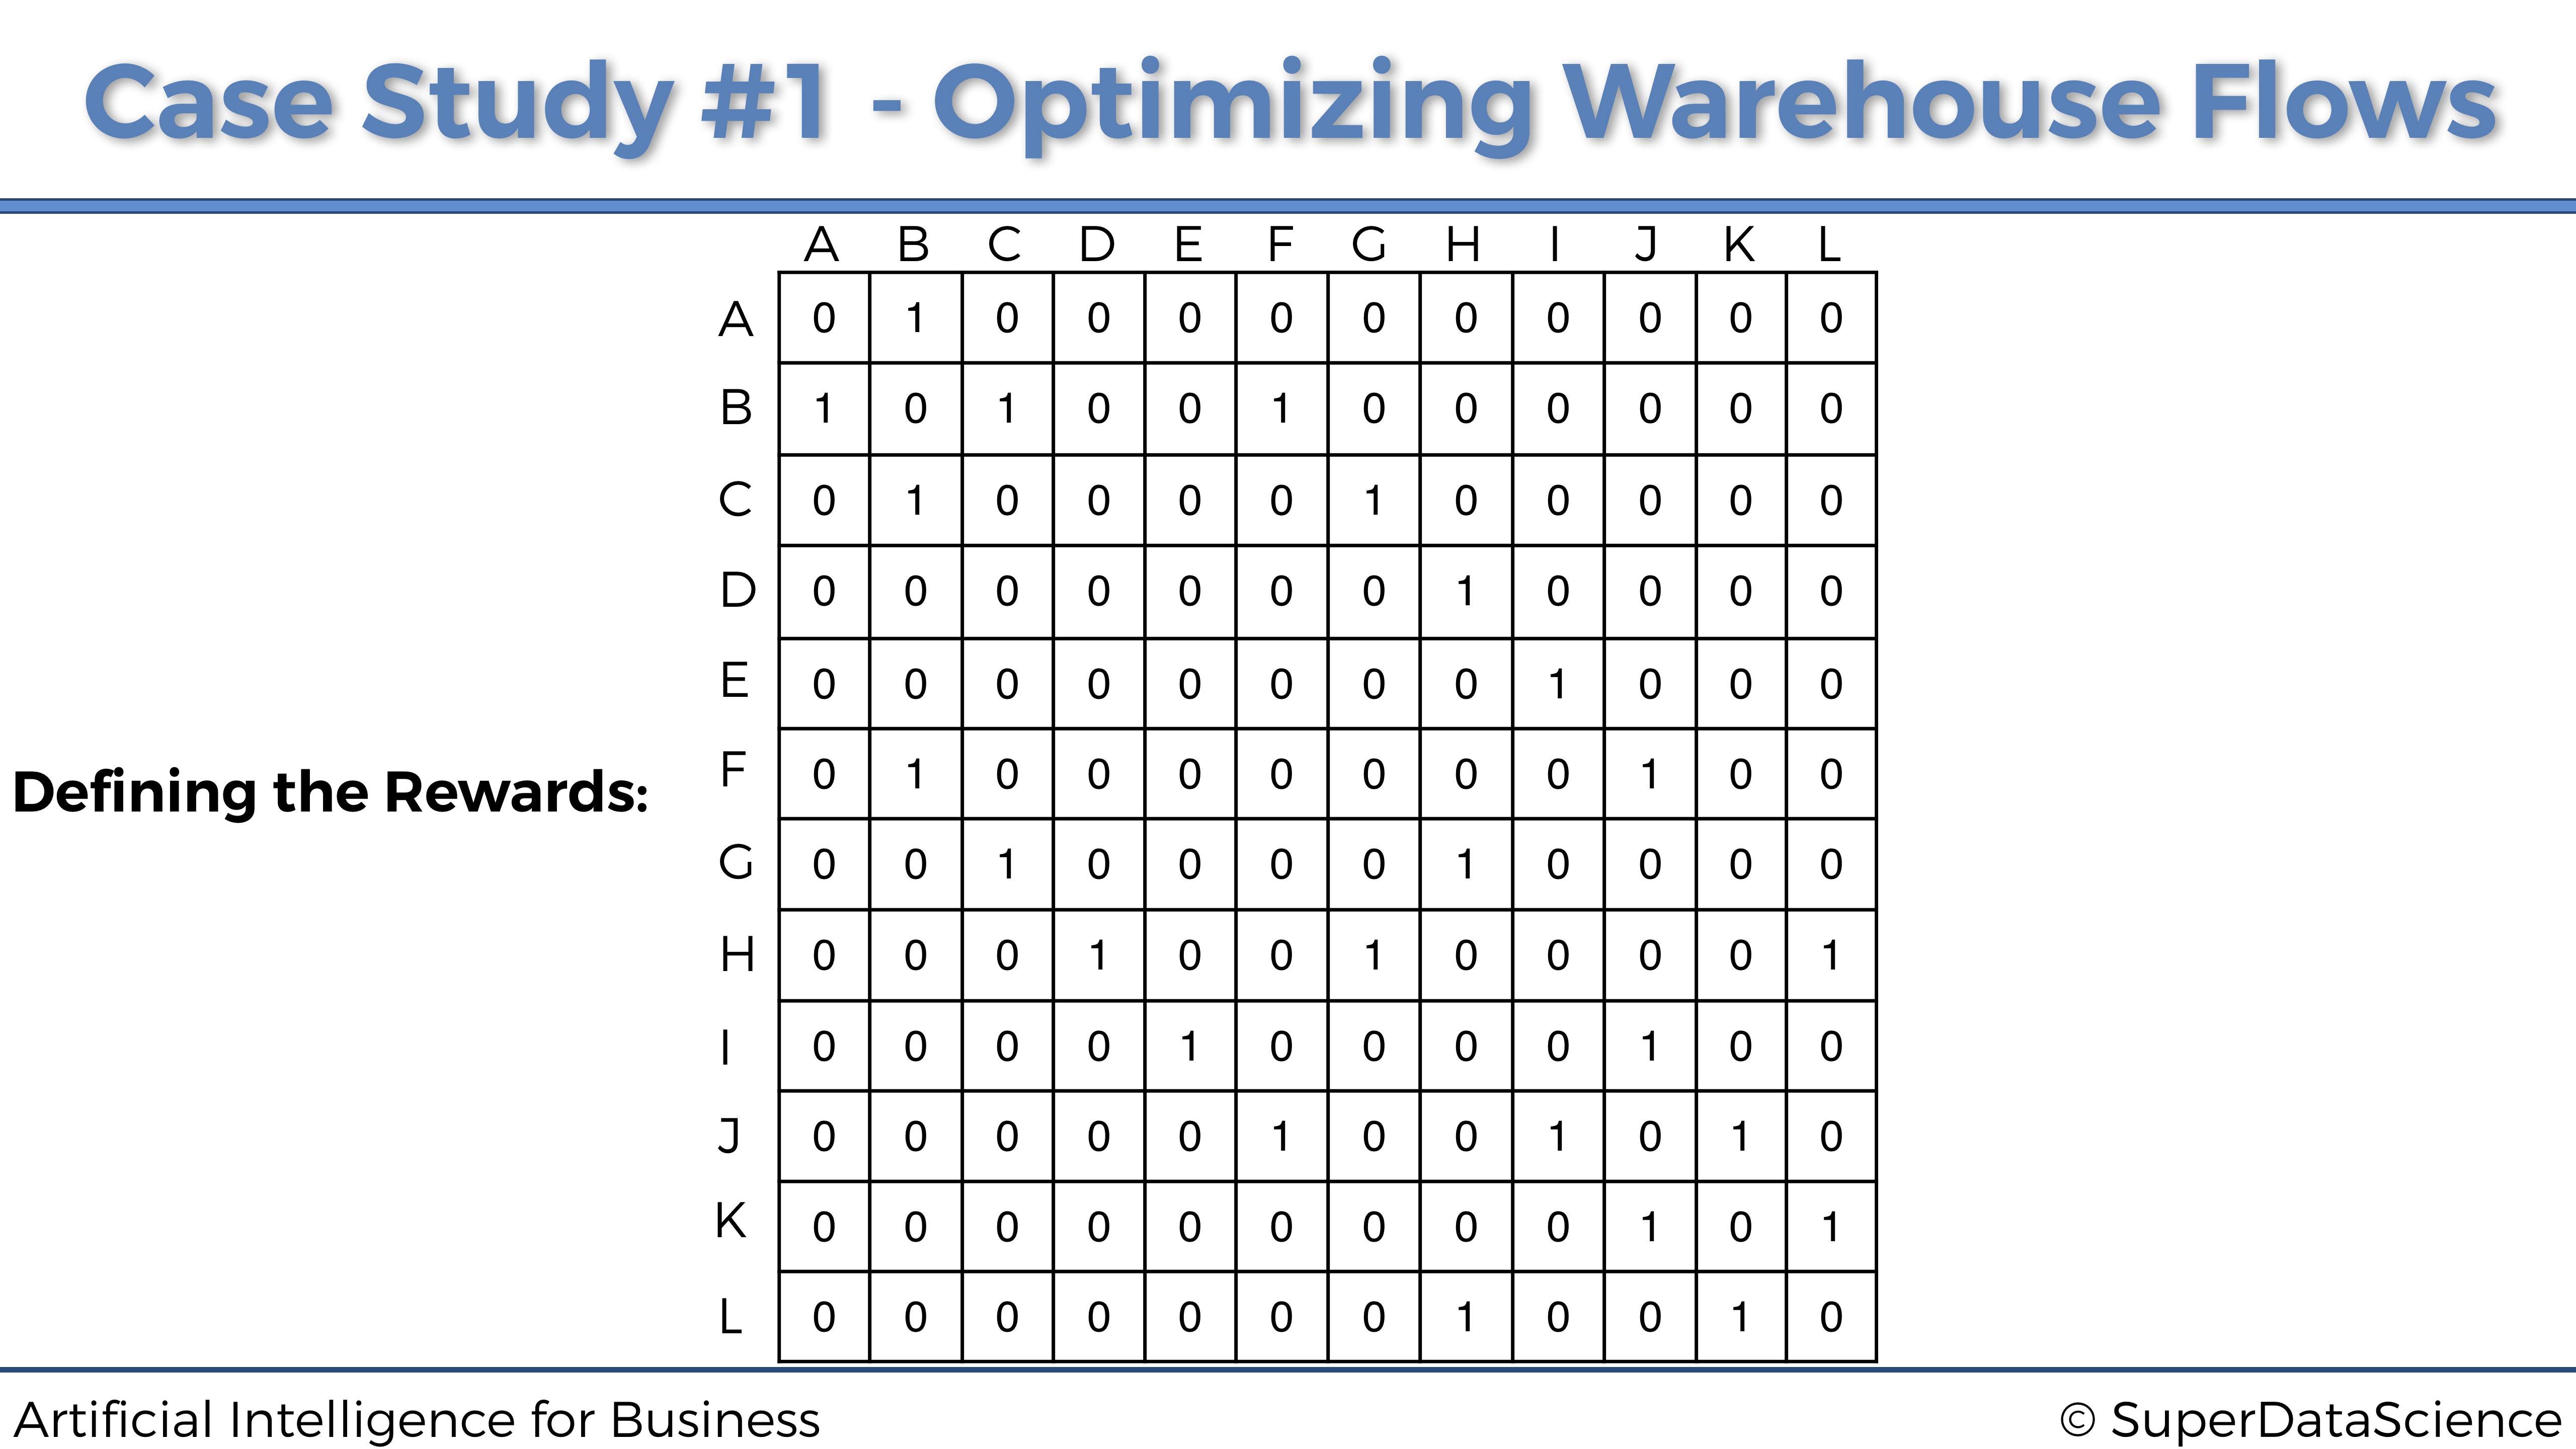
\includegraphics{Images/Rewards_Matrix_4.png}

Felicidades, acabamos de definir las recompensas. Lo hicimos simplemente construyendo esta matriz de recompensas. Es importante entender que esta es la forma en que definimos el sistema de recompensas cuando hacemos Q-Learning con un número finito de entradas y acciones. En el Caso Práctico 2, veremos que procederemos de manera muy diferente.

Ya casi hemos terminado, lo único que tenemos que hacer es atribuir grandes recompensas a las ubicaciones de mayor prioridad. Esto lo hará el sistema informático que devuelve las prioridades de recolección de productos para cada una de las 12 ubicaciones. Por lo tanto, dado que la ubicación G es la máxima prioridad, el sistema informático actualizará la matriz de recompensas atribuyendo una alta recompensa en la celda \((G, G)\):

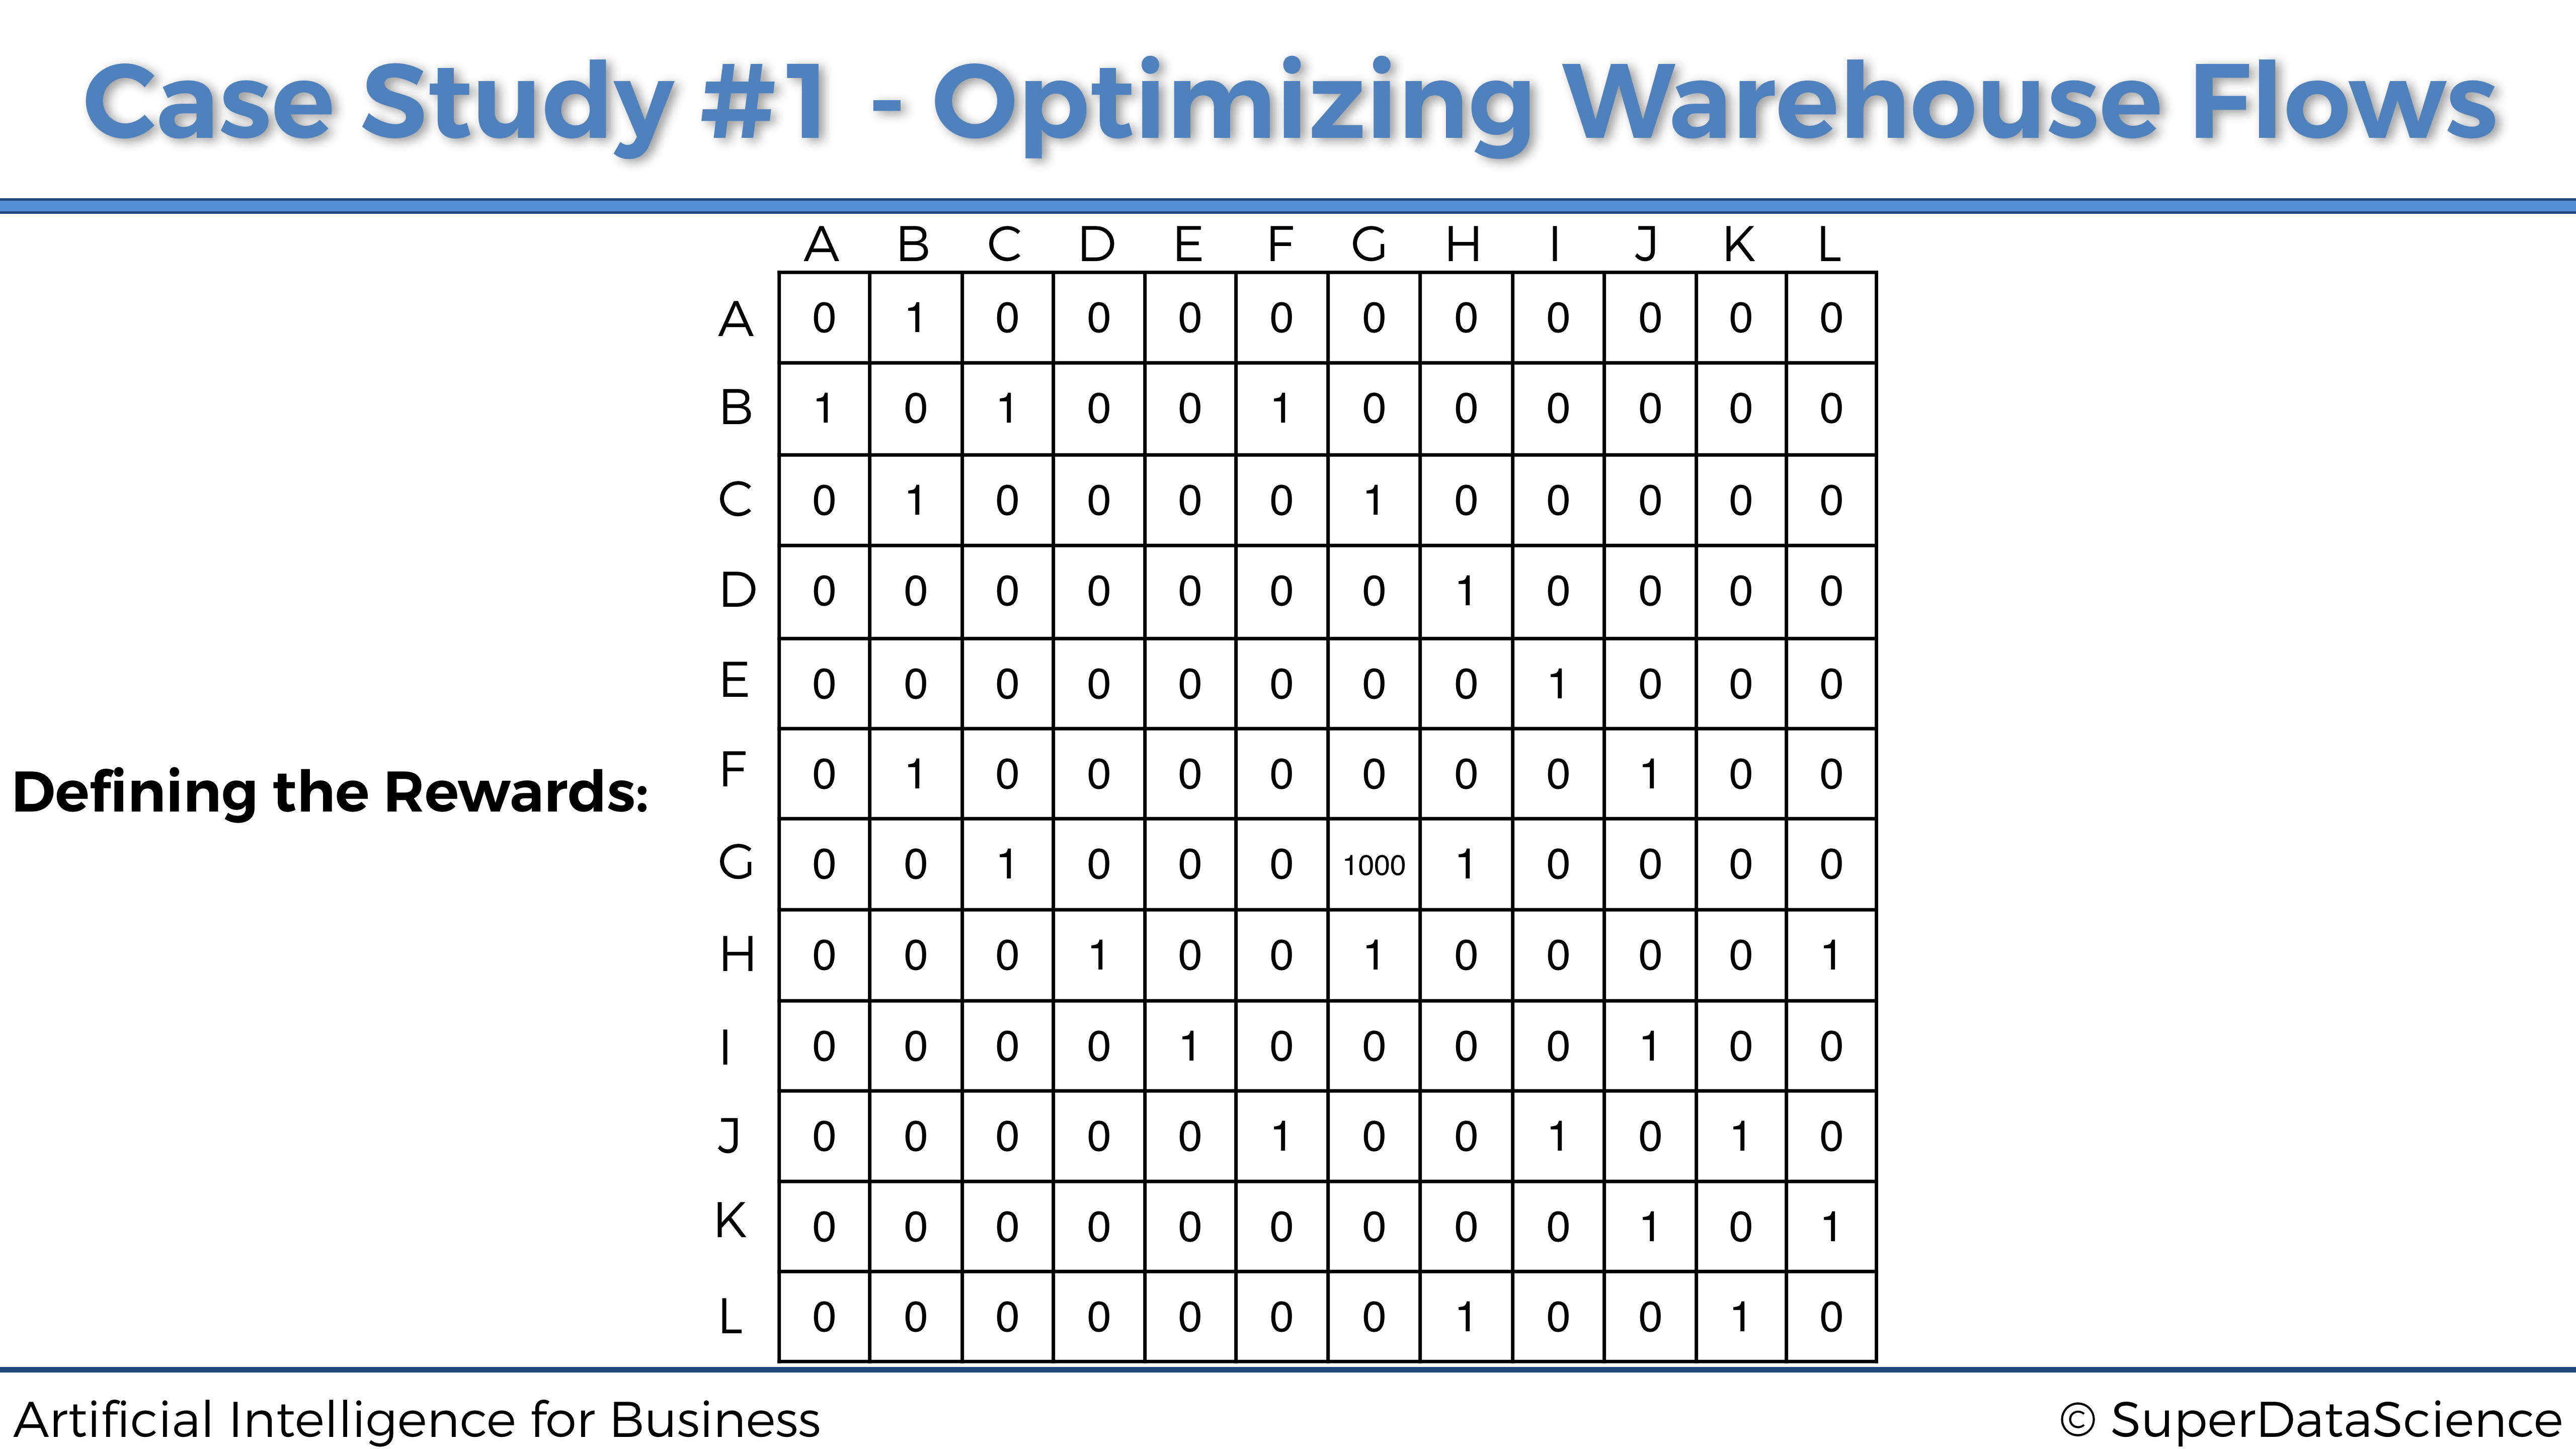
\includegraphics{Images/Rewards_Matrix_5.png}

Y así es como el sistema de recompensas funcionará con Q-Learning. Atribuimos la recompensa más alta (aquí 1000) a la ubicación de máxima prioridad G. Luego puedes ver en las clases de vídeo del curso cómo podemos atribuir una recompensa más alta a la segunda ubicación de mayor prioridad (ubicación K), para hacer que nuestro robot pase por esto ubicación intermedia de máxima prioridad, optimizando así los flujos de movimiento por el almacén.

\hypertarget{soluciuxf3n-de-inteligencia-artificial}{%
\section{Solución de Inteligencia Artificial}\label{soluciuxf3n-de-inteligencia-artificial}}

The AI Solution that will solve the problem described above is a Q-Learning model. Since the latter is based on Markov Decision Processes, or MDPs, we will start by explaining what they are, and then we will move on to the intuition and maths details behind the Q-Learning model.

\hypertarget{proceso-de-decisiuxf3n-de-markov}{%
\subsection{Proceso de Decisión de Markov}\label{proceso-de-decisiuxf3n-de-markov}}

Un Proceso de Decisión de Markov es una tupla \((S, A, T, R)\) donde:

\begin{itemize}
\tightlist
\item
  \(S\) es el conjunto de los diferentes estados. Por lo tanto, en nuestro caso de estudio: \[S = \{0,1,2,3,4,5,6,7,8,9,10,11\}\]
\item
  \(A\) es el conjunto de las diferentes acciones que se pueden llevar a cabo en cada momento \(t\). Por lo tanto, en nuestro caso de estudio: \[A = \{0,1,2,3,4,5,6,7,8,9,10,11\}\]
\item
  \(T\) es la llamada regla de transición:
\end{itemize}

\[T : (s_t \in S, s_{t+1} \in S, a_t \in A) \mapsto \mathbb{P}(s_{t+1}|s_t,a_t)\]

donde \(\mathbb {P} (s_{t + 1} | s_t, a_t)\) es la probabilidad de alcanzar el estado futuro \(s_{t + 1}\) cuando se lleva a cabo la acción \(a_t\) en el estado \(s_t\). Por lo tanto, \(T\) es la distribución de probabilidad de los estados futuros en el tiempo \(t + 1\) dado el estado actual y la acción ejecutada en el tiempo \(t\). En consecuencia, podemos predecir el estado futuro \(s_{t + 1}\) tomando un valor aleatorio de esa distribución \(T\):

\[s_{t+1} \sim T(s_t,.,a_t)\]

En nuestro estudio de caso, verás a través de nuestra implementación que esta distribución \(T\) de nuestra IA simplemente será la distribución uniforme, que es una opción clásica de distribución que funciona muy bien en el marco del Q-Learning.

\begin{itemize}
\tightlist
\item
  \(R\) es la función de recompensas:
\end{itemize}

\[R : (s_t \in S, a_t \in A) \mapsto r_t \in \mathbb{R}\]

donde \(r_t\) es la recompensa obtenida después de ejecutar la acción \(a_t\) en el estado \(s_t\). En nuestro caso práctico, esta función de recompensa es exactamente la matriz que definimos previamente.

Después de definir el proceso de decisión de Markov, ahora es importante recordar que se basa en el siguiente supuesto: la probabilidad del estado futuro \(s_{t + 1}\) solamente depende del estado actual \(s_t\) y la acción ejecutada \(a_t\), y bajo ningun concepto no depende de ninguno de los estados y acciones anteriores. Es decir:

\[\mathbb{P}(s_{t+1}|s_0,a_0,s_1,a_1,...,s_t,a_t) = \mathbb{P}(s_{t+1}|s_t,a_t)\]

En otras palabras, un proceso de decisión de Markov no tiene memoria.

\newpage

Ahora repasemos lo que va a ocurrir en términos de un proceso de decisión de Markov. En cada instante \(t\):

\begin{itemize}
\tightlist
\item
  La IA observa el estado actual \(s_t\).
\item
  La IA ejecuta la acción \(a_t\).
\item
  La IA recibe la recompensa \(r_t = R(s_t, a_t)\).
\item
  La IA entra en el siguiente estado \(s_{t+1}\).
\end{itemize}

Así que la pregunta clave es:

\begin{quote}
\textbf{¿Cómo sabe la IA qué acción llevar a cabo en cada instante \(t\)?}
\end{quote}

Para responder a esta pregunta, necesitamos introducir la función de política. La función de política \(\pi\) es exactamente la función que, dado un estado \(s_t\), devuelve la acción \(a_t\):

\[\pi: s_t \in S \mapsto a_t \in A\]

Denotemos por \(\Pi\) el conjunto de todas las funciones de política posibles. Entonces, la elección de las mejores acciones para jugar se convierte en un problema de optimización. De hecho, se trata de encontrar la política óptima \(\pi^*\) que maximice la recompensa acumulada:

\[\pi^* = \underset{\pi \in \Pi}{\textrm{argmax}} \sum_{t \ge 0} R(s_t,\pi(s_t))\]

Por lo tanto, la pregunta anterior se convierte en:

\begin{quote}
\textbf{¿Cómo encontrar esta política óptima \(\pi^*\)?}
\end{quote}

Aquí es donde entra en juego el Q-Learning.

\hypertarget{q-learning}{%
\subsection{Q-Learning}\label{q-learning}}

Antes de comenzar a entrar en los detalles de Q-Learning, necesitamos explicar el concepto del valor Q.

\textbf{El valor Q}

Para cada par de estado y acción \((s, a)\), vamos a asociar un valor numérico llamado \(Q (s, a)\):

\[Q: (s \in S, a \in A) \mapsto Q(s,a) \in \mathbb{R}\]

Diremos que \(Q (s, a)\) es \emph{el valor Q de la acción \(a\) llevada a cabo en el estado \(s\)}.

Para comprender el propósito de este \emph{Valor Q}, necesitamos introducir la Diferencia Temporal.

\textbf{La Diferencia Temporal}

Al principio \(t = 0\), todos los valores Q se inicializan a 0:

\[\forall s \in S, a \in A, Q(s,a) = 0\]

Ahora supongamos que estamos en el instante \(t\), en cierto estado \(s_t\). Llevamos a cabo una acción aleatoria \(a_t\), que nos lleva al estado \(s_{t + 1}\) y obtenemos la recompensa \(R(s_t, a_t)\).

Ahora podemos presentar la diferencia temporal, que básicamente es el corazón de Q-Learning. La diferencia temporal en el tiempo \(t\), denotada por \(TD_t(s_t, a_t)\), es la diferencia entre:

\begin{itemize}
\item
  \(R(s_t,a_t) + \gamma \underset{a}{\max}(Q(s_{t+1},a))\), es decir la recompensa \(R (s_t, a_t)\) obtenida al llevar a cabo la acción \(a_t\) en el estado \(s_t\), más el valor Q de la mejor acción jugada en el estado futuro \(s_{t + 1}\), descontado por un factor \$\gamma \in [0,1] \$, llamado factor de descuento.
\item
  y \(Q(s_t, a_t)\), es decir el valor Q de la acción \(a_t\) llevada a cabo en el estado \$ s\_t \$,
\end{itemize}

que nos lleva a:

\[TD_t(s_t,a_t) = R(s_t,a_t) + \gamma \underset{a}{\max}(Q(s_{t+1},a)) - Q(s_t,a_t)\]

\begin{quote}
\textbf{Bien, genial, pero ¿cuál es exactamente el propósito de esta diferencia temporal \(TD_t(s_t,a_t)\)?}
\end{quote}

Respondamos esta pregunta para darnos una mejor idea de la IA. \(TD_t (s_t, a_t)\) es como una recompensa intrínseca. La IA aprenderá los valores Q de tal manera que:

\begin{itemize}
\tightlist
\item
  Si \(TD_t(s_t,a_t)\) es alta, la IA recibe una \emph{buena sorpresa}.
\item
  Si \(TD_t(s_t,a_t)\) es alta, la IA recibe \emph{frustración}.
\end{itemize}

En ese sentido, la IA repetirá algunas actualizaciones de los valores Q (a través de una ecuación llamada la ecuación de Bellman) hacia diferencias temporales más altas.

En consecuencia, en el siguiente paso final del algoritmo Q-Learning, usamos la diferencia temporal para reforzar los pares (estado, acción) desde el tiempo \(t-1\) hasta el tiempo \(t\), de acuerdo con la siguiente ecuación:

\[Q_t(s_t,a_t) = Q_{t-1}(s_t,a_t) + \alpha TD_t(s_t,a_t)\]

donde \(\alpha \in \mathbb{R}\) es la tasa de aprendizaje, que determina qué tan rápido va el aprendizaje de los valores Q o qué tan grandes son las actualizaciones de los mismos. Su valor suele ser un número real elegido entre 0 y 1, como por ejemplo 0.01, 0.05, 0.1 o 0.5. Cuanto menor sea su valor, más pequeñas serán las actualizaciones de los valores Q y más larga será la ejecución del algoritmo de Q-Learning. Cuanto mayor sea su valor, mayores serán las actualizaciones de los valores Q y más rápido será el algoritmo de Q-Learning.

Esta ecuación anterior es la ecuación de Bellman. Es el pilar fundamental del Q-Learning.

Con este punto de vista, los valores Q miden la acumulación de sorpresa o frustración asociada con el par de acciones y estados \((s_t, a_t)\). En el caso de recibir sorpresa, la IA se refuerza, y en el caso de recibir frustración, la IA se debilita. Por lo tanto, queremos aprender los valores Q que le darán a la IA la máxima \emph{buena sorpresa}.

En consecuencia, la decisión de qué acción ejecutar depende principalmente del valor Q \(Q(s_t, a_t)\). Si la acción \(a_t\) ejecutada en el estado \(s_t\) está asociada con un valor Q alto \(Q (s_t, a_t)\), la IA tendrá una mayor tendencia a elegir la acción \(a_t\). Por otro lado, si la acción \(a_t\) que se ha llevado a cabo en el estado \(s_t\) está asociada con un valor Q pequeño \(Q(s_t, a_t)\), la IA tendrá una tendencia menor a elegir la acción \(a_t\).

Hay varias formas de elegir la mejor acción para ejecutar en cada esstado. Primero, cuando estamos en cierto estado \(s_t\), simplemente podríamos tomar la acción \(a_t\) que maximiza el valor Q \$ Q(s\_t, a\_t)\$:

\[a_t = \underset{a}{\textrm{argmax}}(Q(s_t,a))\]

Esta solución es el método \textbf{Argmax}.

Otra gran solución, que resulta ser una solución aún mejor para problemas complejos, es el método \textbf{Softmax}.

El método Softmax consiste en considerar para cada estado \(s\) la siguiente distribución:

\[W_s: a \in A \mapsto \frac{\exp(Q(s,a))^{\tau}}{\sum_{a'}\exp(Q(s,a'))^{\tau}} \textrm{ with } \tau \ge 0\]

Luego, elegimos qué acción \(a\) llevar a cabo mediante una muestra de un valor aleatorio de esa distribución:

\[a \sim W_s(.)\]

Sin embargo, el problema que resolveremos en el Caso Práctico 1 será lo suficientemente simple como para usar el método Argmax, así que esto es lo que elegiremos.

\hypertarget{el-algoritmo-de-q-learning-al-completo}{%
\subsection{El algoritmo de Q-Learning al completo}\label{el-algoritmo-de-q-learning-al-completo}}

Resumamos los diferentes pasos de todo el proceso de Q-Learning:

\textbf{Inicialización}

Para todas las parejas de estados \(s\) y acciones \(a\), los valores Q se inicializan a 0:

\[\forall s \in S, a \in A, Q_0(s,a) = 0\]

Comenzamos en el estado inicial \(s_0\). Llevamos a cabo una acción aleatoria posible y llegamos al primer estado \(s_1\).

\textbf{Para cada instante \(t \ge 1\)}, repetiremos un cierto número de veces (1000 veces en nuestro código) lo siguiente:

\begin{itemize}
\tightlist
\item
  Seleccionamos un estado aleatorio \(s_t\) de nuestros 12 estados posibles:
\end{itemize}

\[s_t = \textrm{random}(0,1,2,3,4,5,6,7,8,9,10,11)\]

\begin{itemize}
\tightlist
\item
  Llevamos a cabo una acción aleatoria \(a_t\) que puede conducir al siguiente estado posible, es decir, de modo que \(R(s_t,a_t) > 0\):
\end{itemize}

\[a_t = \textrm{random}(0,1,2,3,4,5,6,7,8,9,10,11) \textrm{ t.q. } R(s_t,a_t) > 0\]

\begin{itemize}
\item
  Llegamos al siguiente estado \(s_{t + 1}\) y obtenemos la recompensa \(R(s_t,a_t)\)
\item
  Calculamos la Diferencia Temporal \(TD_t(s_t,a_t)\):
\end{itemize}

\[TD_t(s_t,a_t) = R(s_t,a_t) + \gamma \underset{a}{\max}(Q(s_{t+1},a)) - Q(s_t, a_t)\]

\begin{itemize}
\tightlist
\item
  Actualizamos el valor Q aplicando la ecuación de Bellman:
\end{itemize}

\[Q_t(s_t,a_t) = Q_{t-1}(s_t,a_t) + \alpha TD_t(s_t,a_t)\]

\hypertarget{implementaciuxf3n}{%
\section{Implementación}\label{implementaciuxf3n}}

Ahora proporcionemos y expliquemos la implementación completa de este modelo de Q-Learning, la solución de nuestro problema de optimización de flujos de almacén.

Primero, comenzamos importando las librerías que se usarán en esta implementación. Estos solo incluyen la biblioteca \texttt{numpy}, que ofrece una forma práctica de trabajar con matrices y operaciones matemáticas:

\begin{Shaded}
\begin{Highlighting}[]
\CommentTok{# Importar las librerías}
\ImportTok{import}\NormalTok{ numpy }\ImportTok{as}\NormalTok{ np}
\end{Highlighting}
\end{Shaded}

Luego establecemos los parámetros de nuestro modelo. Estos incluyen el factor de descuento \(\gamma\) y la tasa de aprendizaje \$\alpha \$, que como vimos en la Sección 1.2, son los únicos parámetros del algoritmo Q-Learning:

\begin{Shaded}
\begin{Highlighting}[]
\CommentTok{# Configuración de los parámetros gamma y alfa para el Q-Learning}
\NormalTok{gamma }\OperatorTok{=} \FloatTok{0.75}
\NormalTok{alpha }\OperatorTok{=} \FloatTok{0.9}
\end{Highlighting}
\end{Shaded}

Las dos secciones de código anteriores eran simplemente las secciones introductorias, antes de comenzar realmente a construir nuestro modelo de IA. Ahora el siguiente paso es comenzar la primera parte de nuestra implementación: Parte 1 - Definición del entorno. Y para eso, por supuesto, comenzamos definiendo los estados, con un diccionario que asigna los nombres de las ubicaciones (en letras de la A a la L) en los estados (en índices del 0 al 11):

\begin{Shaded}
\begin{Highlighting}[]
\CommentTok{# PARTE 1 - DEFINICIÓN DEL ENTORNO}

\CommentTok{# Definición de los estados}
\NormalTok{location_to_state }\OperatorTok{=}\NormalTok{ \{}\StringTok{'A'}\NormalTok{: }\DecValTok{0}\NormalTok{,}
                     \StringTok{'B'}\NormalTok{: }\DecValTok{1}\NormalTok{,}
                     \StringTok{'C'}\NormalTok{: }\DecValTok{2}\NormalTok{,}
                     \StringTok{'D'}\NormalTok{: }\DecValTok{3}\NormalTok{,}
                     \StringTok{'E'}\NormalTok{: }\DecValTok{4}\NormalTok{,}
                     \StringTok{'F'}\NormalTok{: }\DecValTok{5}\NormalTok{,}
                     \StringTok{'G'}\NormalTok{: }\DecValTok{6}\NormalTok{,}
                     \StringTok{'H'}\NormalTok{: }\DecValTok{7}\NormalTok{,}
                     \StringTok{'I'}\NormalTok{: }\DecValTok{8}\NormalTok{,}
                     \StringTok{'J'}\NormalTok{: }\DecValTok{9}\NormalTok{,}
                     \StringTok{'K'}\NormalTok{: }\DecValTok{10}\NormalTok{,}
                     \StringTok{'L'}\NormalTok{: }\DecValTok{11}\NormalTok{\}}
\end{Highlighting}
\end{Shaded}

Luego definimos las acciones, con una simple lista de índices del 0 al 11. Recuerda que cada índice de acción corresponde al siguiente estado (siguiente ubicación) al que conduce dicha acción:

\begin{Shaded}
\begin{Highlighting}[]
\CommentTok{# Definición de las acciones}
\NormalTok{actions }\OperatorTok{=}\NormalTok{ [}\DecValTok{0}\NormalTok{,}\DecValTok{1}\NormalTok{,}\DecValTok{2}\NormalTok{,}\DecValTok{3}\NormalTok{,}\DecValTok{4}\NormalTok{,}\DecValTok{5}\NormalTok{,}\DecValTok{6}\NormalTok{,}\DecValTok{7}\NormalTok{,}\DecValTok{8}\NormalTok{,}\DecValTok{9}\NormalTok{,}\DecValTok{10}\NormalTok{,}\DecValTok{11}\NormalTok{]}
\end{Highlighting}
\end{Shaded}

Y eventualmente, definimos las recompensas, creando una matriz de recompensas, donde las filas corresponden a los estados actuales \(s_t\), las columnas corresponden a las acciones \(a_t\) que conducen al siguiente estado \(s_{t + 1}\), y las celdas contienen las recompensas \(R(s_t, a_t)\). Si una celda \((s_t, a_t)\) tiene un 1, eso significa que podemos llevar a cabo la acción \(a_t\) del estado actual \(s_t\) para llegar al siguiente estado \(s_{t + 1}\). Si una celda \((s_t, a_t)\) tiene un 0, eso significa que no podemos llevar a cabo la acción \(a_t\) del estado actual \(s_t\) para llegar a cualquier estado siguiente \(s_{t + 1}\). Y por ahora colocaremos manualmente una alta recompensa (1000) dentro de la celda correspondiente a la ubicación G, porque es la ubicación de máxima prioridad donde el almacén autónomo tiene que ir a recoger los productos. Como la ubicación G ha codificado el estado como índice 6, colocamos una recompensa de 1000 en la celda de la fila 6 y la columna 6. Luego, mejoraremos nuestra solución al implementar una forma automática de ir a la ubicación de máxima prioridad, sin tener que actualizar manualmente la matriz de recompensas y dejándola inicializada con 0s y 1s como debería ser. Pero mientras tanto, aquí está debajo de nuestra matriz de recompensas, incluida la actualización manual:

\begin{Shaded}
\begin{Highlighting}[]
\CommentTok{# Definición de las recompensas}
\NormalTok{R }\OperatorTok{=}\NormalTok{ np.array([[}\DecValTok{0}\NormalTok{,}\DecValTok{1}\NormalTok{,}\DecValTok{0}\NormalTok{,}\DecValTok{0}\NormalTok{,}\DecValTok{0}\NormalTok{,}\DecValTok{0}\NormalTok{,}\DecValTok{0}\NormalTok{,}\DecValTok{0}\NormalTok{,}\DecValTok{0}\NormalTok{,}\DecValTok{0}\NormalTok{,}\DecValTok{0}\NormalTok{,}\DecValTok{0}\NormalTok{],}
\NormalTok{              [}\DecValTok{1}\NormalTok{,}\DecValTok{0}\NormalTok{,}\DecValTok{1}\NormalTok{,}\DecValTok{0}\NormalTok{,}\DecValTok{0}\NormalTok{,}\DecValTok{1}\NormalTok{,}\DecValTok{0}\NormalTok{,}\DecValTok{0}\NormalTok{,}\DecValTok{0}\NormalTok{,}\DecValTok{0}\NormalTok{,}\DecValTok{0}\NormalTok{,}\DecValTok{0}\NormalTok{],}
\NormalTok{              [}\DecValTok{0}\NormalTok{,}\DecValTok{1}\NormalTok{,}\DecValTok{0}\NormalTok{,}\DecValTok{0}\NormalTok{,}\DecValTok{0}\NormalTok{,}\DecValTok{0}\NormalTok{,}\DecValTok{1}\NormalTok{,}\DecValTok{0}\NormalTok{,}\DecValTok{0}\NormalTok{,}\DecValTok{0}\NormalTok{,}\DecValTok{0}\NormalTok{,}\DecValTok{0}\NormalTok{],}
\NormalTok{              [}\DecValTok{0}\NormalTok{,}\DecValTok{0}\NormalTok{,}\DecValTok{0}\NormalTok{,}\DecValTok{0}\NormalTok{,}\DecValTok{0}\NormalTok{,}\DecValTok{0}\NormalTok{,}\DecValTok{0}\NormalTok{,}\DecValTok{1}\NormalTok{,}\DecValTok{0}\NormalTok{,}\DecValTok{0}\NormalTok{,}\DecValTok{0}\NormalTok{,}\DecValTok{0}\NormalTok{],}
\NormalTok{              [}\DecValTok{0}\NormalTok{,}\DecValTok{0}\NormalTok{,}\DecValTok{0}\NormalTok{,}\DecValTok{0}\NormalTok{,}\DecValTok{0}\NormalTok{,}\DecValTok{0}\NormalTok{,}\DecValTok{0}\NormalTok{,}\DecValTok{0}\NormalTok{,}\DecValTok{1}\NormalTok{,}\DecValTok{0}\NormalTok{,}\DecValTok{0}\NormalTok{,}\DecValTok{0}\NormalTok{],}
\NormalTok{              [}\DecValTok{0}\NormalTok{,}\DecValTok{1}\NormalTok{,}\DecValTok{0}\NormalTok{,}\DecValTok{0}\NormalTok{,}\DecValTok{0}\NormalTok{,}\DecValTok{0}\NormalTok{,}\DecValTok{0}\NormalTok{,}\DecValTok{0}\NormalTok{,}\DecValTok{0}\NormalTok{,}\DecValTok{1}\NormalTok{,}\DecValTok{0}\NormalTok{,}\DecValTok{0}\NormalTok{],}
\NormalTok{              [}\DecValTok{0}\NormalTok{,}\DecValTok{0}\NormalTok{,}\DecValTok{1}\NormalTok{,}\DecValTok{0}\NormalTok{,}\DecValTok{0}\NormalTok{,}\DecValTok{0}\NormalTok{,}\DecValTok{1000}\NormalTok{,}\DecValTok{1}\NormalTok{,}\DecValTok{0}\NormalTok{,}\DecValTok{0}\NormalTok{,}\DecValTok{0}\NormalTok{,}\DecValTok{0}\NormalTok{],}
\NormalTok{              [}\DecValTok{0}\NormalTok{,}\DecValTok{0}\NormalTok{,}\DecValTok{0}\NormalTok{,}\DecValTok{1}\NormalTok{,}\DecValTok{0}\NormalTok{,}\DecValTok{0}\NormalTok{,}\DecValTok{1}\NormalTok{,}\DecValTok{0}\NormalTok{,}\DecValTok{0}\NormalTok{,}\DecValTok{0}\NormalTok{,}\DecValTok{0}\NormalTok{,}\DecValTok{1}\NormalTok{],}
\NormalTok{              [}\DecValTok{0}\NormalTok{,}\DecValTok{0}\NormalTok{,}\DecValTok{0}\NormalTok{,}\DecValTok{0}\NormalTok{,}\DecValTok{1}\NormalTok{,}\DecValTok{0}\NormalTok{,}\DecValTok{0}\NormalTok{,}\DecValTok{0}\NormalTok{,}\DecValTok{0}\NormalTok{,}\DecValTok{1}\NormalTok{,}\DecValTok{0}\NormalTok{,}\DecValTok{0}\NormalTok{],}
\NormalTok{              [}\DecValTok{0}\NormalTok{,}\DecValTok{0}\NormalTok{,}\DecValTok{0}\NormalTok{,}\DecValTok{0}\NormalTok{,}\DecValTok{0}\NormalTok{,}\DecValTok{1}\NormalTok{,}\DecValTok{0}\NormalTok{,}\DecValTok{0}\NormalTok{,}\DecValTok{1}\NormalTok{,}\DecValTok{0}\NormalTok{,}\DecValTok{1}\NormalTok{,}\DecValTok{0}\NormalTok{],}
\NormalTok{              [}\DecValTok{0}\NormalTok{,}\DecValTok{0}\NormalTok{,}\DecValTok{0}\NormalTok{,}\DecValTok{0}\NormalTok{,}\DecValTok{0}\NormalTok{,}\DecValTok{0}\NormalTok{,}\DecValTok{0}\NormalTok{,}\DecValTok{0}\NormalTok{,}\DecValTok{0}\NormalTok{,}\DecValTok{1}\NormalTok{,}\DecValTok{0}\NormalTok{,}\DecValTok{1}\NormalTok{],}
\NormalTok{              [}\DecValTok{0}\NormalTok{,}\DecValTok{0}\NormalTok{,}\DecValTok{0}\NormalTok{,}\DecValTok{0}\NormalTok{,}\DecValTok{0}\NormalTok{,}\DecValTok{0}\NormalTok{,}\DecValTok{0}\NormalTok{,}\DecValTok{1}\NormalTok{,}\DecValTok{0}\NormalTok{,}\DecValTok{0}\NormalTok{,}\DecValTok{1}\NormalTok{,}\DecValTok{0}\NormalTok{]])}
\end{Highlighting}
\end{Shaded}

Eso finaliza esta primera parte. Ahora comencemos la segunda parte de nuestra implementación: Parte 2 - Construcción la solución de IA con Q-Learning. En ese sentido, vamos a seguir el algoritmo de Q-Learning exactamente como lo vimos en la Sección 1.2. Por lo tanto, primero inicializamos todos los valores Q, creando nuestra matriz de valores Q llena de ceros (en los cuales, las filas corresponden a los estados actuales \(s_t\), las columnas corresponden a las acciones \(a_t\) que conducen al siguiente estado \$s\_\{t + 1\} \$, y las celdas contienen los valores Q, \$Q (s\_t, a\_t)) \$:

\begin{Shaded}
\begin{Highlighting}[]
\CommentTok{# PARTE 2 - CONSTRUCCIÓN DE LA SOLUCIÓN DE IA CON Q-LEARNING}

\CommentTok{# Inicialización de los valores Q}
\NormalTok{Q }\OperatorTok{=}\NormalTok{ np.array(np.zeros([}\DecValTok{12}\NormalTok{,}\DecValTok{12}\NormalTok{]))}
\end{Highlighting}
\end{Shaded}

Luego, por supuesto, implementamos el proceso de Q-Learning, con un bucle \texttt{for} que llevará a cabo un total de 1000 iteraciones, repitiendo 1000 veces los pasos del proceso de Q-Learning que analizamos a fondo al final de la Sección 1.2:

\begin{Shaded}
\begin{Highlighting}[]
\CommentTok{# Implementación del proceso de Q-Learning}
\ControlFlowTok{for}\NormalTok{ i }\KeywordTok{in} \BuiltInTok{range}\NormalTok{(}\DecValTok{1000}\NormalTok{):}
\NormalTok{    current_state }\OperatorTok{=}\NormalTok{ np.random.randint(}\DecValTok{0}\NormalTok{,}\DecValTok{12}\NormalTok{)}
\NormalTok{    playable_actions }\OperatorTok{=}\NormalTok{ []}
    \ControlFlowTok{for}\NormalTok{ j }\KeywordTok{in} \BuiltInTok{range}\NormalTok{(}\DecValTok{12}\NormalTok{):}
        \ControlFlowTok{if}\NormalTok{ R[current_state, j] }\OperatorTok{>} \DecValTok{0}\NormalTok{:}
\NormalTok{            playable_actions.append(j)}
\NormalTok{    next_state }\OperatorTok{=}\NormalTok{ np.random.choice(playable_actions)}
\NormalTok{    TD }\OperatorTok{=}\NormalTok{ R[current_state, next_state] }\OperatorTok{+}\NormalTok{ gamma}\OperatorTok{*}\NormalTok{Q[next_state, np.argmax(Q[next_state,])]}
         \OperatorTok{-}\NormalTok{ Q[current_state, next_state]}
\NormalTok{    Q[current_state, next_state] }\OperatorTok{=}\NormalTok{ Q[current_state, next_state] }\OperatorTok{+}\NormalTok{ alpha}\OperatorTok{*}\NormalTok{TD}
\end{Highlighting}
\end{Shaded}

Opcional: en esta etapa del código, nuestra matriz de valores Q está lista. Podemos echarle un vistazo ejecutando todo el código que hemos implementado hasta ahora e ingresando las siguientes dos instrucciones en la consola:

\begin{Shaded}
\begin{Highlighting}[]
\BuiltInTok{print}\NormalTok{(}\StringTok{"Q-Values:"}\NormalTok{)}
\BuiltInTok{print}\NormalTok{(Q.astype(}\BuiltInTok{int}\NormalTok{))}
\end{Highlighting}
\end{Shaded}

Y obtenemos la siguiente matriz de valores Q finales:

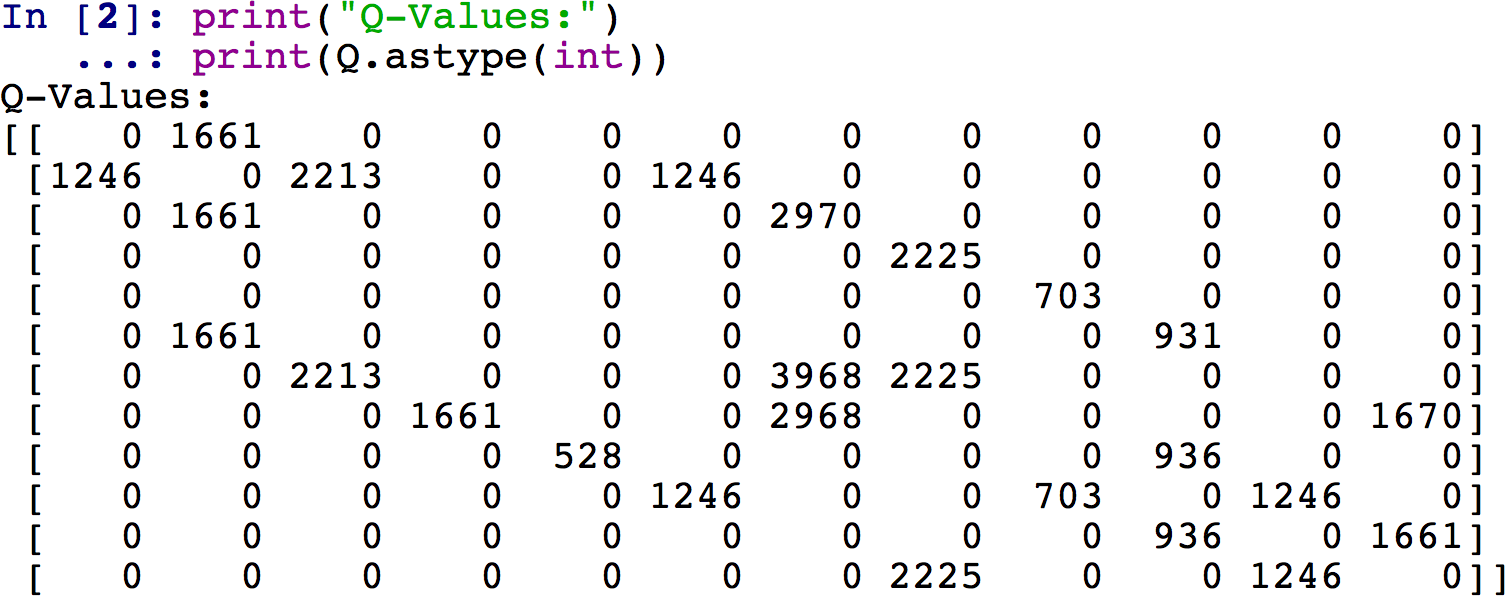
\includegraphics{Images/Q_Values_Console.png}

Para una mayor claridad visual, incluso puede verificarse la matriz de valores Q directamente en el Explorador de variables, haciendo doble clic en la variable Q. Luego, para obtener los valores Q como enteros, es conveniente hacer clic en \texttt{Formato} e ingresar un formato de como floante como \texttt{\%.0f}. Se obtiene en este caso el siguiente resultado, que es un poco más claro ya que se pueden ver en la matriz Q los índices de las filas y columnas de la misma:

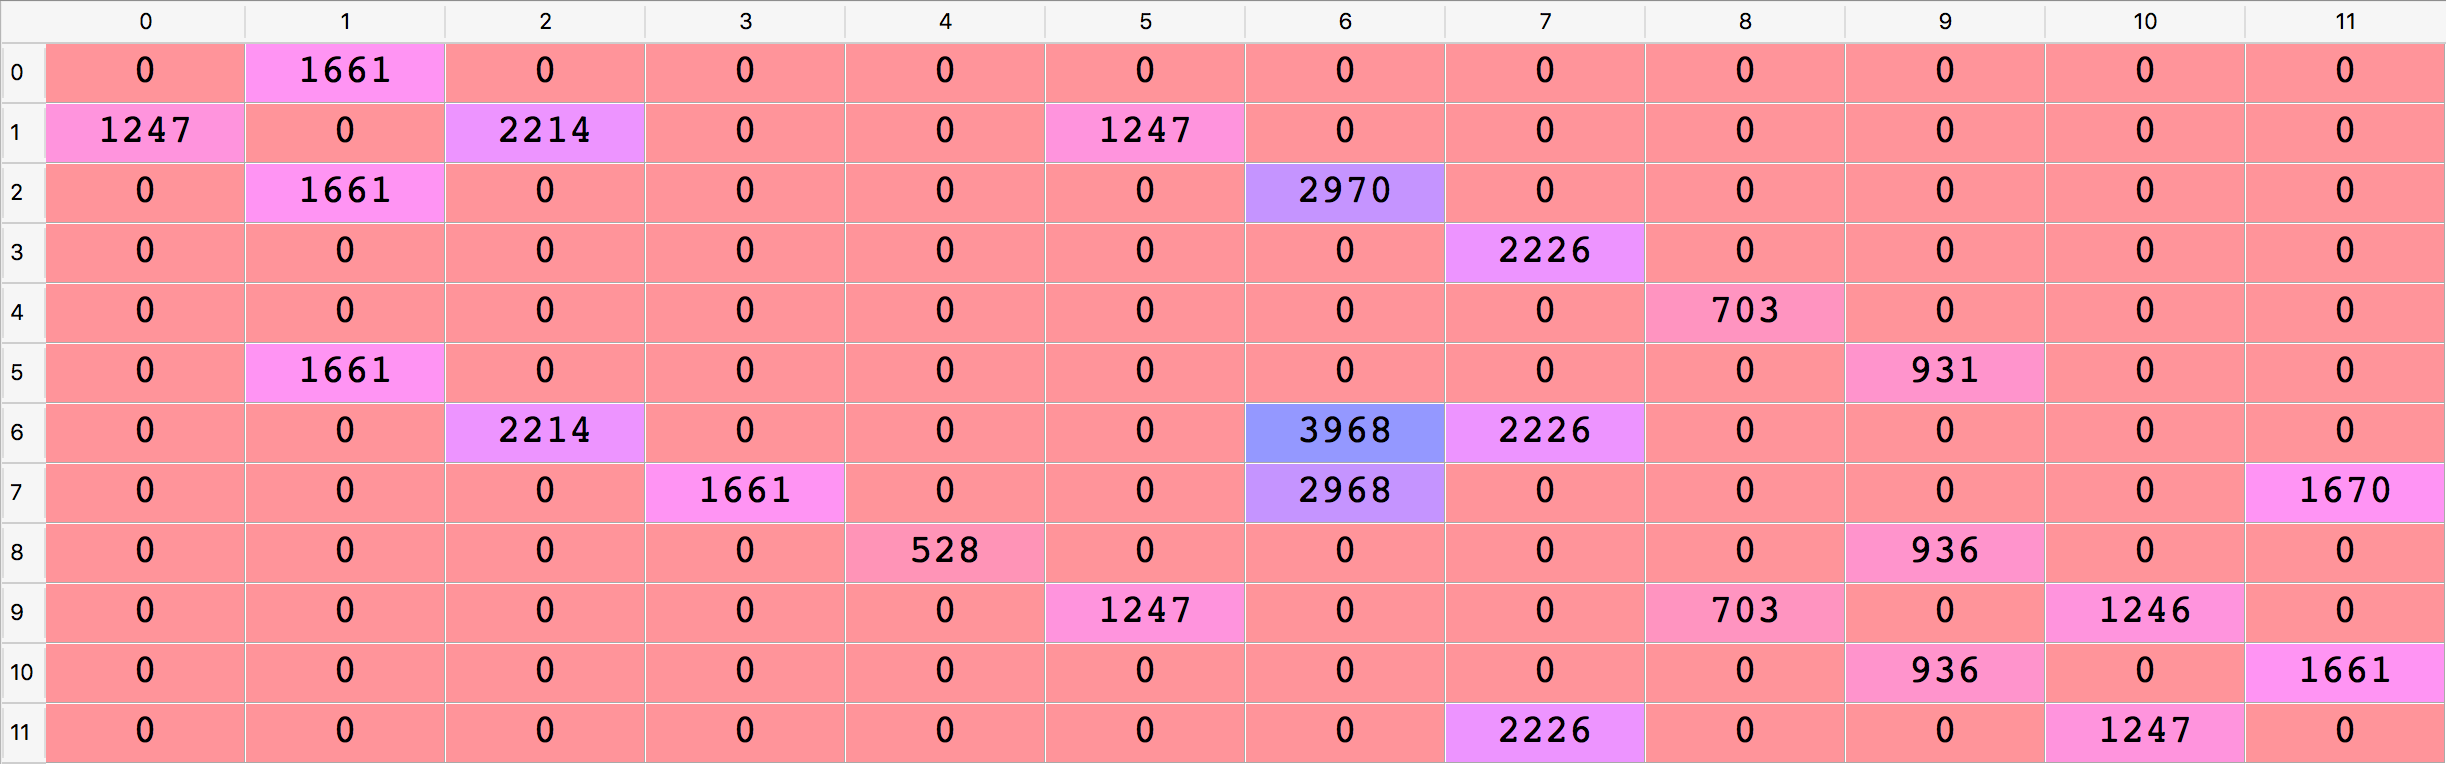
\includegraphics{Images/Q_Values_Variable_Explorer.png}

Bien, ahora que tenemos nuestra matriz de valores Q, ¡estamos listos para llevarlo a producción! Por lo tanto, podemos pasar a la tercera parte de la implementación, Parte 3: Poner el modelo en producción, dentro de la cual calcularemos la ruta óptima desde cualquier ubicación inicial a cualquier ubicación final de máxima prioridad. La idea aquí será implementar una función de \emph{ruta}, que tomará como entradas la ubicación de inicio donde se encuentra nuestro robot de almacén autónomo en un momento específico y la ubicación de finalización donde tiene que ir con la máxima prioridad, y eso volverá como genera la ruta más corta dentro de una lista. Sin embargo, dado que queremos indicar las ubicaciones con sus nombres (en letras), a diferencia de sus estados (en índices), necesitaremos un diccionario que asigne los estados de ubicaciones (en índices) a los nombres de ubicaciones (en letras). Y eso es lo primero que haremos aquí en esta tercera parte, usando un truco para invertir nuestro diccionario anterior \texttt{location\textbackslash{}\_to\textbackslash{}\_state}, ya que de hecho simplemente queremos obtener el mapeo inverso exacto de este diccionario:

\begin{Shaded}
\begin{Highlighting}[]
\CommentTok{# PARTE 3 - PONER EL MODELO EN PRODUCCIÓN}

\CommentTok{# Hacer un mapeo de los estados a las ubicaciones}
\NormalTok{state_to_location }\OperatorTok{=}\NormalTok{ \{state: location }\ControlFlowTok{for}\NormalTok{ location, state }\KeywordTok{in}\NormalTok{ location_to_state.items()\}}
\end{Highlighting}
\end{Shaded}

Aquí es cuando entra en juego la sección de código más importante. Estamos a punto de implementar la función final \texttt{route\ ()} que tomará como entradas las ubicaciones de inicio y finalización, y que devolverá la ruta óptima entre estas dos ubicaciones. Para explicar exactamente qué hará esta función de ruta, enumeremos los diferentes pasos del proceso, al pasar de la ubicación E a la ubicación G:

\begin{enumerate}
\def\labelenumi{\arabic{enumi}.}
\tightlist
\item
  Comenzamos en nuestra ubicación inicial E.
\item
  Obtenemos el estado de ubicación E, que según nuestro mapeo \texttt{location\_to\_state} es \(s_0 = 4\).
\item
  En la fila del estado \(s_0 = 4\) de nuestra matriz de valores Q, hallamos la columna con el mayor valor Q (703).
\item
  Esta columna tiene el índice 8, por lo que ejecutamos la acción del índice 8 que nos lleva al siguiente estado \(s_{t+1} = 8\).
\item
  Obtenemos la ubicación del estado 8, que según nuestro mapeo \texttt{state\_to\_location} es la ubicación I. Por lo tanto, nuestra próxima ubicación es la ubicación I, que se adjunta a nuestra lista que contiene la ruta óptima global.
\item
  Repetimos los mismos 5 pasos anteriores desde nuestra nueva ubicación inicial I, hasta llegar a nuestro destino final, la ubicación G.
\end{enumerate}

Por lo tanto, dado que no sabemos cuántas ubicaciones tendremos que atravesar entre las ubicaciones inicial y final, tenemos que hacer un bucle \texttt{while} que repetirá el proceso de 5 pasos descrito anteriormente, y que se detendrá tan pronto como lo hagamos llegar a la ubicación final de máxima prioridad:

\begin{Shaded}
\begin{Highlighting}[]
\CommentTok{# Hacer la función final que devolverá la ruta óptima}
\KeywordTok{def}\NormalTok{ route(starting_location, ending_location):}
\NormalTok{    route }\OperatorTok{=}\NormalTok{ [starting_location]}
\NormalTok{    next_location }\OperatorTok{=}\NormalTok{ starting_location}
    \ControlFlowTok{while}\NormalTok{ (next_location }\OperatorTok{!=}\NormalTok{ ending_location):}
\NormalTok{        starting_state }\OperatorTok{=}\NormalTok{ location_to_state[starting_location]}
\NormalTok{        next_state }\OperatorTok{=}\NormalTok{ np.argmax(Q[starting_state,])}
\NormalTok{        next_location }\OperatorTok{=}\NormalTok{ state_to_location[next_state]}
\NormalTok{        route.append(next_location)}
\NormalTok{        starting_location }\OperatorTok{=}\NormalTok{ next_location}
    \ControlFlowTok{return}\NormalTok{ route}
\end{Highlighting}
\end{Shaded}

¡Felicidades, nuestra herramienta ya está lista! Cuando lo probamos para ir de E a G, obtenemos las dos rutas óptimas posibles después de imprimir la ruta final ejecutando el código completo varias veces:

\begin{Shaded}
\begin{Highlighting}[]
\CommentTok{# Imprimir la ruta final}
\BuiltInTok{print}\NormalTok{(}\StringTok{'Route:'}\NormalTok{)}
\NormalTok{route(}\StringTok{'E'}\NormalTok{, }\StringTok{'G'}\NormalTok{)}
\end{Highlighting}
\end{Shaded}

\begin{Shaded}
\begin{Highlighting}[]
\NormalTok{Route:}
\NormalTok{Out[}\DecValTok{1}\NormalTok{]: [}\StringTok{'E'}\NormalTok{, }\StringTok{'I'}\NormalTok{, }\StringTok{'J'}\NormalTok{, }\StringTok{'F'}\NormalTok{, }\StringTok{'B'}\NormalTok{, }\StringTok{'C'}\NormalTok{, }\StringTok{'G'}\NormalTok{]}
\NormalTok{Out[}\DecValTok{2}\NormalTok{]: [}\StringTok{'E'}\NormalTok{, }\StringTok{'I'}\NormalTok{, }\StringTok{'J'}\NormalTok{, }\StringTok{'K'}\NormalTok{, }\StringTok{'L'}\NormalTok{, }\StringTok{'H'}\NormalTok{, }\StringTok{'G'}\NormalTok{]}
\end{Highlighting}
\end{Shaded}

Bien, tenemos una primera versión del modelo que funciona bien. Pero podemos mejorarlo de dos maneras. Primero, al automatizar la atribución de recompensas a la ubicación de máxima prioridad, para que no tengamos que hacerlo manualmente. Y segundo, al agregar una función que nos da la opción de ir a una ubicación intermedia antes de ir a la ubicación de máxima prioridad. Esa ubicación intermedia debe estar, por supuesto, en las 3 ubicaciones prioritarias principales. Y, de hecho, en nuestra clasificación de ubicaciones de máxima prioridad, la segunda ubicación de máxima prioridad es la ubicación K. Por lo tanto, para optimizar aún más los flujos de almacén, nuestro robot de almacén autónomo debe ir por la ubicación K para recoger los productos en su camino a la ubicación de máxima prioridad G. Una forma de hacer esto es tener la opción de ir a cualquier ubicación intermedia en el proceso de nuestra función \texttt{route()}. Y esto es exactamente lo que implementaremos como segunda mejora. Pero primero, implementemos la primera mejora, que automatiza la atribución de recompensas.

La forma de hacerlo es en dos pasos: primero debemos hacer una copia (llamada \texttt{R\_new}) de nuestra matriz de recompensa dentro de la cual la función \texttt{route()} actualizará automáticamente la recompensa en la celda de la ubicación final. De hecho, la ubicación final es una de las entradas de la función \texttt{route()}, por lo que al usar nuestro diccionario de \texttt{location\_to\_state} podemos encontrar fácilmente esa celda y actualizar su recompensa a 1000. Y segundo, debemos incluir toda la lógica del algoritmo de Q-learning (incluido el paso de inicialización) dentro de la función de ruta, justo después de hacer esa actualización de la recompensa en nuestra copia de la matriz de recompensas. De hecho, en nuestra implementación anterior anterior, el proceso de Q-Learning ocurre en la versión original de la matriz de recompensas, que ahora se supone que permanece como está, es decir, se inicializa solo a 1s y 0s. Por lo tanto, debemos incluir el proceso de Q-Learning dentro de la función de ruta y hacer que suceda en nuestra copia \texttt{R\_new} de la matriz de recompensas, en lugar de la matriz de recompensas original \texttt{R}. Por lo tanto, nuestra implementación completa se convierte en lo siguiente:

\begin{Shaded}
\begin{Highlighting}[]
\CommentTok{# Inteligencia Artificial aplicada a Negocios y Empresas}

\CommentTok{# Optimización de Procesos en un almacén con Q-Learning}

\CommentTok{# # Importar las librerías}
\ImportTok{import}\NormalTok{ numpy }\ImportTok{as}\NormalTok{ np}

\CommentTok{# Configuración de los parámetros gamma y alfa para el Q-Learning}
\NormalTok{gamma }\OperatorTok{=} \FloatTok{0.75}
\NormalTok{alpha }\OperatorTok{=} \FloatTok{0.9}

\CommentTok{# PARTE 1 - DEFINICIÓN DEL ENTORNO}

\CommentTok{# Definición de los estados}
\NormalTok{location_to_state }\OperatorTok{=}\NormalTok{ \{}\StringTok{'A'}\NormalTok{: }\DecValTok{0}\NormalTok{,}
                     \StringTok{'B'}\NormalTok{: }\DecValTok{1}\NormalTok{,}
                     \StringTok{'C'}\NormalTok{: }\DecValTok{2}\NormalTok{,}
                     \StringTok{'D'}\NormalTok{: }\DecValTok{3}\NormalTok{,}
                     \StringTok{'E'}\NormalTok{: }\DecValTok{4}\NormalTok{,}
                     \StringTok{'F'}\NormalTok{: }\DecValTok{5}\NormalTok{,}
                     \StringTok{'G'}\NormalTok{: }\DecValTok{6}\NormalTok{,}
                     \StringTok{'H'}\NormalTok{: }\DecValTok{7}\NormalTok{,}
                     \StringTok{'I'}\NormalTok{: }\DecValTok{8}\NormalTok{,}
                     \StringTok{'J'}\NormalTok{: }\DecValTok{9}\NormalTok{,}
                     \StringTok{'K'}\NormalTok{: }\DecValTok{10}\NormalTok{,}
                     \StringTok{'L'}\NormalTok{: }\DecValTok{11}\NormalTok{\}}

\CommentTok{# Definición de las acciones}
\NormalTok{actions }\OperatorTok{=}\NormalTok{ [}\DecValTok{0}\NormalTok{,}\DecValTok{1}\NormalTok{,}\DecValTok{2}\NormalTok{,}\DecValTok{3}\NormalTok{,}\DecValTok{4}\NormalTok{,}\DecValTok{5}\NormalTok{,}\DecValTok{6}\NormalTok{,}\DecValTok{7}\NormalTok{,}\DecValTok{8}\NormalTok{,}\DecValTok{9}\NormalTok{,}\DecValTok{10}\NormalTok{,}\DecValTok{11}\NormalTok{]}

\CommentTok{# Definición de las recompensas}
\NormalTok{R }\OperatorTok{=}\NormalTok{ np.array([[}\DecValTok{0}\NormalTok{,}\DecValTok{1}\NormalTok{,}\DecValTok{0}\NormalTok{,}\DecValTok{0}\NormalTok{,}\DecValTok{0}\NormalTok{,}\DecValTok{0}\NormalTok{,}\DecValTok{0}\NormalTok{,}\DecValTok{0}\NormalTok{,}\DecValTok{0}\NormalTok{,}\DecValTok{0}\NormalTok{,}\DecValTok{0}\NormalTok{,}\DecValTok{0}\NormalTok{],}
\NormalTok{              [}\DecValTok{1}\NormalTok{,}\DecValTok{0}\NormalTok{,}\DecValTok{1}\NormalTok{,}\DecValTok{0}\NormalTok{,}\DecValTok{0}\NormalTok{,}\DecValTok{1}\NormalTok{,}\DecValTok{0}\NormalTok{,}\DecValTok{0}\NormalTok{,}\DecValTok{0}\NormalTok{,}\DecValTok{0}\NormalTok{,}\DecValTok{0}\NormalTok{,}\DecValTok{0}\NormalTok{],}
\NormalTok{              [}\DecValTok{0}\NormalTok{,}\DecValTok{1}\NormalTok{,}\DecValTok{0}\NormalTok{,}\DecValTok{0}\NormalTok{,}\DecValTok{0}\NormalTok{,}\DecValTok{0}\NormalTok{,}\DecValTok{1}\NormalTok{,}\DecValTok{0}\NormalTok{,}\DecValTok{0}\NormalTok{,}\DecValTok{0}\NormalTok{,}\DecValTok{0}\NormalTok{,}\DecValTok{0}\NormalTok{],}
\NormalTok{              [}\DecValTok{0}\NormalTok{,}\DecValTok{0}\NormalTok{,}\DecValTok{0}\NormalTok{,}\DecValTok{0}\NormalTok{,}\DecValTok{0}\NormalTok{,}\DecValTok{0}\NormalTok{,}\DecValTok{0}\NormalTok{,}\DecValTok{1}\NormalTok{,}\DecValTok{0}\NormalTok{,}\DecValTok{0}\NormalTok{,}\DecValTok{0}\NormalTok{,}\DecValTok{0}\NormalTok{],}
\NormalTok{              [}\DecValTok{0}\NormalTok{,}\DecValTok{0}\NormalTok{,}\DecValTok{0}\NormalTok{,}\DecValTok{0}\NormalTok{,}\DecValTok{0}\NormalTok{,}\DecValTok{0}\NormalTok{,}\DecValTok{0}\NormalTok{,}\DecValTok{0}\NormalTok{,}\DecValTok{1}\NormalTok{,}\DecValTok{0}\NormalTok{,}\DecValTok{0}\NormalTok{,}\DecValTok{0}\NormalTok{],}
\NormalTok{              [}\DecValTok{0}\NormalTok{,}\DecValTok{1}\NormalTok{,}\DecValTok{0}\NormalTok{,}\DecValTok{0}\NormalTok{,}\DecValTok{0}\NormalTok{,}\DecValTok{0}\NormalTok{,}\DecValTok{0}\NormalTok{,}\DecValTok{0}\NormalTok{,}\DecValTok{0}\NormalTok{,}\DecValTok{1}\NormalTok{,}\DecValTok{0}\NormalTok{,}\DecValTok{0}\NormalTok{],}
\NormalTok{              [}\DecValTok{0}\NormalTok{,}\DecValTok{0}\NormalTok{,}\DecValTok{1}\NormalTok{,}\DecValTok{0}\NormalTok{,}\DecValTok{0}\NormalTok{,}\DecValTok{0}\NormalTok{,}\DecValTok{1}\NormalTok{,}\DecValTok{1}\NormalTok{,}\DecValTok{0}\NormalTok{,}\DecValTok{0}\NormalTok{,}\DecValTok{0}\NormalTok{,}\DecValTok{0}\NormalTok{],}
\NormalTok{              [}\DecValTok{0}\NormalTok{,}\DecValTok{0}\NormalTok{,}\DecValTok{0}\NormalTok{,}\DecValTok{1}\NormalTok{,}\DecValTok{0}\NormalTok{,}\DecValTok{0}\NormalTok{,}\DecValTok{1}\NormalTok{,}\DecValTok{0}\NormalTok{,}\DecValTok{0}\NormalTok{,}\DecValTok{0}\NormalTok{,}\DecValTok{0}\NormalTok{,}\DecValTok{1}\NormalTok{],}
\NormalTok{              [}\DecValTok{0}\NormalTok{,}\DecValTok{0}\NormalTok{,}\DecValTok{0}\NormalTok{,}\DecValTok{0}\NormalTok{,}\DecValTok{1}\NormalTok{,}\DecValTok{0}\NormalTok{,}\DecValTok{0}\NormalTok{,}\DecValTok{0}\NormalTok{,}\DecValTok{0}\NormalTok{,}\DecValTok{1}\NormalTok{,}\DecValTok{0}\NormalTok{,}\DecValTok{0}\NormalTok{],}
\NormalTok{              [}\DecValTok{0}\NormalTok{,}\DecValTok{0}\NormalTok{,}\DecValTok{0}\NormalTok{,}\DecValTok{0}\NormalTok{,}\DecValTok{0}\NormalTok{,}\DecValTok{1}\NormalTok{,}\DecValTok{0}\NormalTok{,}\DecValTok{0}\NormalTok{,}\DecValTok{1}\NormalTok{,}\DecValTok{0}\NormalTok{,}\DecValTok{1}\NormalTok{,}\DecValTok{0}\NormalTok{],}
\NormalTok{              [}\DecValTok{0}\NormalTok{,}\DecValTok{0}\NormalTok{,}\DecValTok{0}\NormalTok{,}\DecValTok{0}\NormalTok{,}\DecValTok{0}\NormalTok{,}\DecValTok{0}\NormalTok{,}\DecValTok{0}\NormalTok{,}\DecValTok{0}\NormalTok{,}\DecValTok{0}\NormalTok{,}\DecValTok{1}\NormalTok{,}\DecValTok{0}\NormalTok{,}\DecValTok{1}\NormalTok{],}
\NormalTok{              [}\DecValTok{0}\NormalTok{,}\DecValTok{0}\NormalTok{,}\DecValTok{0}\NormalTok{,}\DecValTok{0}\NormalTok{,}\DecValTok{0}\NormalTok{,}\DecValTok{0}\NormalTok{,}\DecValTok{0}\NormalTok{,}\DecValTok{1}\NormalTok{,}\DecValTok{0}\NormalTok{,}\DecValTok{0}\NormalTok{,}\DecValTok{1}\NormalTok{,}\DecValTok{0}\NormalTok{]])}

\CommentTok{# PARTE 2 - CONSTRUCCIÓN DE LA SOLUCIÓN DE IA CON Q-LEARNING}

\CommentTok{# Crear una función de mapping desde los estados a las ubicaciones}
\NormalTok{state_to_location }\OperatorTok{=}\NormalTok{ \{state: location }\ControlFlowTok{for}\NormalTok{ location, state }\KeywordTok{in}\NormalTok{ location_to_state.items()\}}

\CommentTok{# Crear una función que devuelva el camino más corto desde la ubicación inicial a la final}
\KeywordTok{def}\NormalTok{ route(starting_location, ending_location):}
\NormalTok{    R_new }\OperatorTok{=}\NormalTok{ np.copy(R)}
\NormalTok{    ending_state }\OperatorTok{=}\NormalTok{ location_to_state[ending_location]}
\NormalTok{    R_new[ending_state, ending_state] }\OperatorTok{=} \DecValTok{1000}
\NormalTok{    Q }\OperatorTok{=}\NormalTok{ np.array(np.zeros([}\DecValTok{12}\NormalTok{,}\DecValTok{12}\NormalTok{]))}
    \ControlFlowTok{for}\NormalTok{ i }\KeywordTok{in} \BuiltInTok{range}\NormalTok{(}\DecValTok{1000}\NormalTok{):}
\NormalTok{        current_state }\OperatorTok{=}\NormalTok{ np.random.randint(}\DecValTok{0}\NormalTok{,}\DecValTok{12}\NormalTok{)}
\NormalTok{        playable_actions }\OperatorTok{=}\NormalTok{ []}
        \ControlFlowTok{for}\NormalTok{ j }\KeywordTok{in} \BuiltInTok{range}\NormalTok{(}\DecValTok{12}\NormalTok{):}
            \ControlFlowTok{if}\NormalTok{ R_new[current_state, j] }\OperatorTok{>} \DecValTok{0}\NormalTok{:}
\NormalTok{                playable_actions.append(j)}
\NormalTok{        next_state }\OperatorTok{=}\NormalTok{ np.random.choice(playable_actions)}
\NormalTok{        TD }\OperatorTok{=}\NormalTok{ R_new[current_state, next_state]}
             \OperatorTok{+}\NormalTok{ gamma }\OperatorTok{*}\NormalTok{ Q[next_state, np.argmax(Q[next_state,])]}
             \OperatorTok{-}\NormalTok{ Q[current_state, next_state]}
\NormalTok{        Q[current_state, next_state] }\OperatorTok{=}\NormalTok{ Q[current_state, next_state] }\OperatorTok{+}\NormalTok{ alpha }\OperatorTok{*}\NormalTok{ TD}
\NormalTok{    route }\OperatorTok{=}\NormalTok{ [starting_location]}
\NormalTok{    next_location }\OperatorTok{=}\NormalTok{ starting_location}
    \ControlFlowTok{while}\NormalTok{ (next_location }\OperatorTok{!=}\NormalTok{ ending_location):}
\NormalTok{        starting_state }\OperatorTok{=}\NormalTok{ location_to_state[starting_location]}
\NormalTok{        next_state }\OperatorTok{=}\NormalTok{ np.argmax(Q[starting_state,])}
\NormalTok{        next_location }\OperatorTok{=}\NormalTok{ state_to_location[next_state]}
\NormalTok{        route.append(next_location)}
\NormalTok{        starting_location }\OperatorTok{=}\NormalTok{ next_location}
    \ControlFlowTok{return}\NormalTok{ route}

\CommentTok{# PARTE 3 - PONER EL MODELO EN PRODUCCIÓN}

\CommentTok{# Imprimir la ruta final}
\BuiltInTok{print}\NormalTok{(}\StringTok{'Route:'}\NormalTok{)}
\NormalTok{route(}\StringTok{'E'}\NormalTok{, }\StringTok{'G'}\NormalTok{)}
\end{Highlighting}
\end{Shaded}

Al ejecutar este nuevo código varias veces, obtenemos, por supuesto, las mismas dos posibles rutas óptimas que antes.

Ahora abordemos la segunda mejora. Hay tres formas de agregar la opción de ir por la ubicación intermedia K, la segunda ubicación de máxima prioridad:

\begin{enumerate}
\def\labelenumi{\arabic{enumi}.}
\tightlist
\item
  Otorgamos una alta recompensa a la acción que lleva de la ubicación J a la ubicación K. Esta alta recompensa debe ser mayor que 1 y menor a 1000. De hecho, debe ser mayor que 1 para que el proceso de Q-Learning favorezca la acción que lleva de J a K, en oposición a la acción que lleva de J a F que tiene la recompensa 1. Y debe ser inferior a 1000, por lo que debemos mantener la recompensa más alta en la ubicación de mayor prioridad para asegurarnos de que terminemos allí. Por lo tanto, por ejemplo, en nuestra matriz de recompensas podemos dar una alta recompensa de 500 a la celda en la fila del índice 9 y la columna del índice 10, ya que de hecho esa celda corresponde a la acción que conduce desde la ubicación J (índice de estado 9) a ubicación K (índice de estado 10). De esa manera, nuestro robot de almacén autónomo siempre irá por la ubicación K en su camino hacia la ubicación G. Así es como sería la matriz de recompensas en ese caso:
\end{enumerate}

\begin{Shaded}
\begin{Highlighting}[]
\CommentTok{# Definición de las recompensas}
\NormalTok{R }\OperatorTok{=}\NormalTok{ np.array([[}\DecValTok{0}\NormalTok{,}\DecValTok{1}\NormalTok{,}\DecValTok{0}\NormalTok{,}\DecValTok{0}\NormalTok{,}\DecValTok{0}\NormalTok{,}\DecValTok{0}\NormalTok{,}\DecValTok{0}\NormalTok{,}\DecValTok{0}\NormalTok{,}\DecValTok{0}\NormalTok{,}\DecValTok{0}\NormalTok{,}\DecValTok{0}\NormalTok{,}\DecValTok{0}\NormalTok{],}
\NormalTok{          [}\DecValTok{1}\NormalTok{,}\DecValTok{0}\NormalTok{,}\DecValTok{1}\NormalTok{,}\DecValTok{0}\NormalTok{,}\DecValTok{0}\NormalTok{,}\DecValTok{1}\NormalTok{,}\DecValTok{0}\NormalTok{,}\DecValTok{0}\NormalTok{,}\DecValTok{0}\NormalTok{,}\DecValTok{0}\NormalTok{,}\DecValTok{0}\NormalTok{,}\DecValTok{0}\NormalTok{],}
\NormalTok{          [}\DecValTok{0}\NormalTok{,}\DecValTok{1}\NormalTok{,}\DecValTok{0}\NormalTok{,}\DecValTok{0}\NormalTok{,}\DecValTok{0}\NormalTok{,}\DecValTok{0}\NormalTok{,}\DecValTok{1}\NormalTok{,}\DecValTok{0}\NormalTok{,}\DecValTok{0}\NormalTok{,}\DecValTok{0}\NormalTok{,}\DecValTok{0}\NormalTok{,}\DecValTok{0}\NormalTok{],}
\NormalTok{          [}\DecValTok{0}\NormalTok{,}\DecValTok{0}\NormalTok{,}\DecValTok{0}\NormalTok{,}\DecValTok{0}\NormalTok{,}\DecValTok{0}\NormalTok{,}\DecValTok{0}\NormalTok{,}\DecValTok{0}\NormalTok{,}\DecValTok{1}\NormalTok{,}\DecValTok{0}\NormalTok{,}\DecValTok{0}\NormalTok{,}\DecValTok{0}\NormalTok{,}\DecValTok{0}\NormalTok{],}
\NormalTok{          [}\DecValTok{0}\NormalTok{,}\DecValTok{0}\NormalTok{,}\DecValTok{0}\NormalTok{,}\DecValTok{0}\NormalTok{,}\DecValTok{0}\NormalTok{,}\DecValTok{0}\NormalTok{,}\DecValTok{0}\NormalTok{,}\DecValTok{0}\NormalTok{,}\DecValTok{1}\NormalTok{,}\DecValTok{0}\NormalTok{,}\DecValTok{0}\NormalTok{,}\DecValTok{0}\NormalTok{],}
\NormalTok{          [}\DecValTok{0}\NormalTok{,}\DecValTok{1}\NormalTok{,}\DecValTok{0}\NormalTok{,}\DecValTok{0}\NormalTok{,}\DecValTok{0}\NormalTok{,}\DecValTok{0}\NormalTok{,}\DecValTok{0}\NormalTok{,}\DecValTok{0}\NormalTok{,}\DecValTok{0}\NormalTok{,}\DecValTok{1}\NormalTok{,}\DecValTok{0}\NormalTok{,}\DecValTok{0}\NormalTok{],}
\NormalTok{          [}\DecValTok{0}\NormalTok{,}\DecValTok{0}\NormalTok{,}\DecValTok{1}\NormalTok{,}\DecValTok{0}\NormalTok{,}\DecValTok{0}\NormalTok{,}\DecValTok{0}\NormalTok{,}\DecValTok{1}\NormalTok{,}\DecValTok{1}\NormalTok{,}\DecValTok{0}\NormalTok{,}\DecValTok{0}\NormalTok{,}\DecValTok{0}\NormalTok{,}\DecValTok{0}\NormalTok{],}
\NormalTok{          [}\DecValTok{0}\NormalTok{,}\DecValTok{0}\NormalTok{,}\DecValTok{0}\NormalTok{,}\DecValTok{1}\NormalTok{,}\DecValTok{0}\NormalTok{,}\DecValTok{0}\NormalTok{,}\DecValTok{1}\NormalTok{,}\DecValTok{0}\NormalTok{,}\DecValTok{0}\NormalTok{,}\DecValTok{0}\NormalTok{,}\DecValTok{0}\NormalTok{,}\DecValTok{1}\NormalTok{],}
\NormalTok{          [}\DecValTok{0}\NormalTok{,}\DecValTok{0}\NormalTok{,}\DecValTok{0}\NormalTok{,}\DecValTok{0}\NormalTok{,}\DecValTok{1}\NormalTok{,}\DecValTok{0}\NormalTok{,}\DecValTok{0}\NormalTok{,}\DecValTok{0}\NormalTok{,}\DecValTok{0}\NormalTok{,}\DecValTok{1}\NormalTok{,}\DecValTok{0}\NormalTok{,}\DecValTok{0}\NormalTok{],}
\NormalTok{          [}\DecValTok{0}\NormalTok{,}\DecValTok{0}\NormalTok{,}\DecValTok{0}\NormalTok{,}\DecValTok{0}\NormalTok{,}\DecValTok{0}\NormalTok{,}\DecValTok{1}\NormalTok{,}\DecValTok{0}\NormalTok{,}\DecValTok{0}\NormalTok{,}\DecValTok{1}\NormalTok{,}\DecValTok{0}\NormalTok{,}\DecValTok{500}\NormalTok{,}\DecValTok{0}\NormalTok{],}
\NormalTok{          [}\DecValTok{0}\NormalTok{,}\DecValTok{0}\NormalTok{,}\DecValTok{0}\NormalTok{,}\DecValTok{0}\NormalTok{,}\DecValTok{0}\NormalTok{,}\DecValTok{0}\NormalTok{,}\DecValTok{0}\NormalTok{,}\DecValTok{0}\NormalTok{,}\DecValTok{0}\NormalTok{,}\DecValTok{1}\NormalTok{,}\DecValTok{0}\NormalTok{,}\DecValTok{1}\NormalTok{],}
\NormalTok{          [}\DecValTok{0}\NormalTok{,}\DecValTok{0}\NormalTok{,}\DecValTok{0}\NormalTok{,}\DecValTok{0}\NormalTok{,}\DecValTok{0}\NormalTok{,}\DecValTok{0}\NormalTok{,}\DecValTok{0}\NormalTok{,}\DecValTok{1}\NormalTok{,}\DecValTok{0}\NormalTok{,}\DecValTok{0}\NormalTok{,}\DecValTok{1}\NormalTok{,}\DecValTok{0}\NormalTok{]])}
\end{Highlighting}
\end{Shaded}

\begin{enumerate}
\def\labelenumi{\arabic{enumi}.}
\setcounter{enumi}{1}
\tightlist
\item
  Damos una mala recompensa a la acción que lleva de la ubicación J a la ubicación F. Esta mala recompensa solo tiene que ser inferior a 0. De hecho, al castigar esta acción con una mala recompensa, el proceso de Q-Learning nunca favorecerá esa acción que lleva de J a F. Por lo tanto, por ejemplo, en nuestra matriz de recompensas podemos dar una mala recompensa de -500 a la celda en la fila del índice 9 y la columna del índice 5, ya que esa celda corresponde a la acción que conduce desde la ubicación J (estado con índice 9) a la ubicación F (estado con índice 5). De esa manera, nuestro robot de almacén autónomo nunca pasará por la ubicación F en su camino hacia la ubicación G. Así es como sería la matriz de recompensas en ese caso:
\end{enumerate}

\begin{Shaded}
\begin{Highlighting}[]
\CommentTok{# Definición de las recompensas}
\NormalTok{R }\OperatorTok{=}\NormalTok{ np.array([[}\DecValTok{0}\NormalTok{,}\DecValTok{1}\NormalTok{,}\DecValTok{0}\NormalTok{,}\DecValTok{0}\NormalTok{,}\DecValTok{0}\NormalTok{,}\DecValTok{0}\NormalTok{,}\DecValTok{0}\NormalTok{,}\DecValTok{0}\NormalTok{,}\DecValTok{0}\NormalTok{,}\DecValTok{0}\NormalTok{,}\DecValTok{0}\NormalTok{,}\DecValTok{0}\NormalTok{],}
\NormalTok{          [}\DecValTok{1}\NormalTok{,}\DecValTok{0}\NormalTok{,}\DecValTok{1}\NormalTok{,}\DecValTok{0}\NormalTok{,}\DecValTok{0}\NormalTok{,}\DecValTok{1}\NormalTok{,}\DecValTok{0}\NormalTok{,}\DecValTok{0}\NormalTok{,}\DecValTok{0}\NormalTok{,}\DecValTok{0}\NormalTok{,}\DecValTok{0}\NormalTok{,}\DecValTok{0}\NormalTok{],}
\NormalTok{          [}\DecValTok{0}\NormalTok{,}\DecValTok{1}\NormalTok{,}\DecValTok{0}\NormalTok{,}\DecValTok{0}\NormalTok{,}\DecValTok{0}\NormalTok{,}\DecValTok{0}\NormalTok{,}\DecValTok{1}\NormalTok{,}\DecValTok{0}\NormalTok{,}\DecValTok{0}\NormalTok{,}\DecValTok{0}\NormalTok{,}\DecValTok{0}\NormalTok{,}\DecValTok{0}\NormalTok{],}
\NormalTok{          [}\DecValTok{0}\NormalTok{,}\DecValTok{0}\NormalTok{,}\DecValTok{0}\NormalTok{,}\DecValTok{0}\NormalTok{,}\DecValTok{0}\NormalTok{,}\DecValTok{0}\NormalTok{,}\DecValTok{0}\NormalTok{,}\DecValTok{1}\NormalTok{,}\DecValTok{0}\NormalTok{,}\DecValTok{0}\NormalTok{,}\DecValTok{0}\NormalTok{,}\DecValTok{0}\NormalTok{],}
\NormalTok{          [}\DecValTok{0}\NormalTok{,}\DecValTok{0}\NormalTok{,}\DecValTok{0}\NormalTok{,}\DecValTok{0}\NormalTok{,}\DecValTok{0}\NormalTok{,}\DecValTok{0}\NormalTok{,}\DecValTok{0}\NormalTok{,}\DecValTok{0}\NormalTok{,}\DecValTok{1}\NormalTok{,}\DecValTok{0}\NormalTok{,}\DecValTok{0}\NormalTok{,}\DecValTok{0}\NormalTok{],}
\NormalTok{          [}\DecValTok{0}\NormalTok{,}\DecValTok{1}\NormalTok{,}\DecValTok{0}\NormalTok{,}\DecValTok{0}\NormalTok{,}\DecValTok{0}\NormalTok{,}\DecValTok{0}\NormalTok{,}\DecValTok{0}\NormalTok{,}\DecValTok{0}\NormalTok{,}\DecValTok{0}\NormalTok{,}\DecValTok{1}\NormalTok{,}\DecValTok{0}\NormalTok{,}\DecValTok{0}\NormalTok{],}
\NormalTok{          [}\DecValTok{0}\NormalTok{,}\DecValTok{0}\NormalTok{,}\DecValTok{1}\NormalTok{,}\DecValTok{0}\NormalTok{,}\DecValTok{0}\NormalTok{,}\DecValTok{0}\NormalTok{,}\DecValTok{1}\NormalTok{,}\DecValTok{1}\NormalTok{,}\DecValTok{0}\NormalTok{,}\DecValTok{0}\NormalTok{,}\DecValTok{0}\NormalTok{,}\DecValTok{0}\NormalTok{],}
\NormalTok{          [}\DecValTok{0}\NormalTok{,}\DecValTok{0}\NormalTok{,}\DecValTok{0}\NormalTok{,}\DecValTok{1}\NormalTok{,}\DecValTok{0}\NormalTok{,}\DecValTok{0}\NormalTok{,}\DecValTok{1}\NormalTok{,}\DecValTok{0}\NormalTok{,}\DecValTok{0}\NormalTok{,}\DecValTok{0}\NormalTok{,}\DecValTok{0}\NormalTok{,}\DecValTok{1}\NormalTok{],}
\NormalTok{          [}\DecValTok{0}\NormalTok{,}\DecValTok{0}\NormalTok{,}\DecValTok{0}\NormalTok{,}\DecValTok{0}\NormalTok{,}\DecValTok{1}\NormalTok{,}\DecValTok{0}\NormalTok{,}\DecValTok{0}\NormalTok{,}\DecValTok{0}\NormalTok{,}\DecValTok{0}\NormalTok{,}\DecValTok{1}\NormalTok{,}\DecValTok{0}\NormalTok{,}\DecValTok{0}\NormalTok{],}
\NormalTok{          [}\DecValTok{0}\NormalTok{,}\DecValTok{0}\NormalTok{,}\DecValTok{0}\NormalTok{,}\DecValTok{0}\NormalTok{,}\DecValTok{0}\NormalTok{,}\OperatorTok{-}\DecValTok{500}\NormalTok{,}\DecValTok{0}\NormalTok{,}\DecValTok{0}\NormalTok{,}\DecValTok{1}\NormalTok{,}\DecValTok{0}\NormalTok{,}\DecValTok{1}\NormalTok{,}\DecValTok{0}\NormalTok{],}
\NormalTok{          [}\DecValTok{0}\NormalTok{,}\DecValTok{0}\NormalTok{,}\DecValTok{0}\NormalTok{,}\DecValTok{0}\NormalTok{,}\DecValTok{0}\NormalTok{,}\DecValTok{0}\NormalTok{,}\DecValTok{0}\NormalTok{,}\DecValTok{0}\NormalTok{,}\DecValTok{0}\NormalTok{,}\DecValTok{1}\NormalTok{,}\DecValTok{0}\NormalTok{,}\DecValTok{1}\NormalTok{],}
\NormalTok{          [}\DecValTok{0}\NormalTok{,}\DecValTok{0}\NormalTok{,}\DecValTok{0}\NormalTok{,}\DecValTok{0}\NormalTok{,}\DecValTok{0}\NormalTok{,}\DecValTok{0}\NormalTok{,}\DecValTok{0}\NormalTok{,}\DecValTok{1}\NormalTok{,}\DecValTok{0}\NormalTok{,}\DecValTok{0}\NormalTok{,}\DecValTok{1}\NormalTok{,}\DecValTok{0}\NormalTok{]])}
\end{Highlighting}
\end{Shaded}

\begin{enumerate}
\def\labelenumi{\arabic{enumi}.}
\setcounter{enumi}{2}
\tightlist
\item
  Realizamos una función adicional \texttt{best\_route()}, tomando como entradas las tres ubicaciones inicial, intermedia y final, que llamará a nuestra función \texttt{route()} anterior dos veces, una primera vez desde la ubicación inicial a la ubicación intermedia, y un segunda vez desde la ubicación intermedia hasta la ubicación final.
\end{enumerate}

Las dos primeras ideas son fáciles de implementar manualmente, pero muy difíciles de implementar automáticamente. De hecho, es fácil encontrar automáticamente el índice de la ubicación intermedia donde queremos ir, pero es muy difícil obtener el índice de la ubicación que lleva a esa ubicación intermedia, ya que depende de la ubicación inicial y la ubicación final. Puedes intentar implementar la primera o la segunda idea, y verás lo que quiero decir. En consecuencia, implementaremos la tercera idea, que puede programarse en solo dos líneas adicionales de código:

\begin{Shaded}
\begin{Highlighting}[]
\CommentTok{# Hacer la función final que devuelve la ruta óptima}
\KeywordTok{def}\NormalTok{ best_route(starting_location, intermediary_location, ending_location):}
    \ControlFlowTok{return}\NormalTok{ route(starting_location, intermediary_location)}
           \OperatorTok{+}\NormalTok{ route(intermediary_location, ending_location)[}\DecValTok{1}\NormalTok{:]}
\end{Highlighting}
\end{Shaded}

Finalmente, el código final que incluye esa mejora importante para la optimización de los flujos de nuestro almacén se convierte en:

\begin{Shaded}
\begin{Highlighting}[]
\CommentTok{# Inteligencia Artificial aplicada a Negocios y Empresas}
\CommentTok{# Optimización de Procesos en un almacén con Q-Learning}

\CommentTok{# # Importar las librerías}
\ImportTok{import}\NormalTok{ numpy }\ImportTok{as}\NormalTok{ np}

\CommentTok{# Configuración de los parámetros gamma y alfa para el Q-Learning}
\NormalTok{gamma }\OperatorTok{=} \FloatTok{0.75}
\NormalTok{alpha }\OperatorTok{=} \FloatTok{0.9}

\CommentTok{# PARTE 1 - DEFINICIÓN DEL ENTORNO}

\CommentTok{# Definición de los estados}
\NormalTok{location_to_state }\OperatorTok{=}\NormalTok{ \{}\StringTok{'A'}\NormalTok{: }\DecValTok{0}\NormalTok{,}
                     \StringTok{'B'}\NormalTok{: }\DecValTok{1}\NormalTok{,}
                     \StringTok{'C'}\NormalTok{: }\DecValTok{2}\NormalTok{,}
                     \StringTok{'D'}\NormalTok{: }\DecValTok{3}\NormalTok{,}
                     \StringTok{'E'}\NormalTok{: }\DecValTok{4}\NormalTok{,}
                     \StringTok{'F'}\NormalTok{: }\DecValTok{5}\NormalTok{,}
                     \StringTok{'G'}\NormalTok{: }\DecValTok{6}\NormalTok{,}
                     \StringTok{'H'}\NormalTok{: }\DecValTok{7}\NormalTok{,}
                     \StringTok{'I'}\NormalTok{: }\DecValTok{8}\NormalTok{,}
                     \StringTok{'J'}\NormalTok{: }\DecValTok{9}\NormalTok{,}
                     \StringTok{'K'}\NormalTok{: }\DecValTok{10}\NormalTok{,}
                     \StringTok{'L'}\NormalTok{: }\DecValTok{11}\NormalTok{\}}

\CommentTok{# Definición de las acciones}
\NormalTok{actions }\OperatorTok{=}\NormalTok{ [}\DecValTok{0}\NormalTok{,}\DecValTok{1}\NormalTok{,}\DecValTok{2}\NormalTok{,}\DecValTok{3}\NormalTok{,}\DecValTok{4}\NormalTok{,}\DecValTok{5}\NormalTok{,}\DecValTok{6}\NormalTok{,}\DecValTok{7}\NormalTok{,}\DecValTok{8}\NormalTok{,}\DecValTok{9}\NormalTok{,}\DecValTok{10}\NormalTok{,}\DecValTok{11}\NormalTok{]}

\CommentTok{# Definición de las recompensas}
\NormalTok{R }\OperatorTok{=}\NormalTok{ np.array([[}\DecValTok{0}\NormalTok{,}\DecValTok{1}\NormalTok{,}\DecValTok{0}\NormalTok{,}\DecValTok{0}\NormalTok{,}\DecValTok{0}\NormalTok{,}\DecValTok{0}\NormalTok{,}\DecValTok{0}\NormalTok{,}\DecValTok{0}\NormalTok{,}\DecValTok{0}\NormalTok{,}\DecValTok{0}\NormalTok{,}\DecValTok{0}\NormalTok{,}\DecValTok{0}\NormalTok{],}
\NormalTok{              [}\DecValTok{1}\NormalTok{,}\DecValTok{0}\NormalTok{,}\DecValTok{1}\NormalTok{,}\DecValTok{0}\NormalTok{,}\DecValTok{0}\NormalTok{,}\DecValTok{1}\NormalTok{,}\DecValTok{0}\NormalTok{,}\DecValTok{0}\NormalTok{,}\DecValTok{0}\NormalTok{,}\DecValTok{0}\NormalTok{,}\DecValTok{0}\NormalTok{,}\DecValTok{0}\NormalTok{],}
\NormalTok{              [}\DecValTok{0}\NormalTok{,}\DecValTok{1}\NormalTok{,}\DecValTok{0}\NormalTok{,}\DecValTok{0}\NormalTok{,}\DecValTok{0}\NormalTok{,}\DecValTok{0}\NormalTok{,}\DecValTok{1}\NormalTok{,}\DecValTok{0}\NormalTok{,}\DecValTok{0}\NormalTok{,}\DecValTok{0}\NormalTok{,}\DecValTok{0}\NormalTok{,}\DecValTok{0}\NormalTok{],}
\NormalTok{              [}\DecValTok{0}\NormalTok{,}\DecValTok{0}\NormalTok{,}\DecValTok{0}\NormalTok{,}\DecValTok{0}\NormalTok{,}\DecValTok{0}\NormalTok{,}\DecValTok{0}\NormalTok{,}\DecValTok{0}\NormalTok{,}\DecValTok{1}\NormalTok{,}\DecValTok{0}\NormalTok{,}\DecValTok{0}\NormalTok{,}\DecValTok{0}\NormalTok{,}\DecValTok{0}\NormalTok{],}
\NormalTok{              [}\DecValTok{0}\NormalTok{,}\DecValTok{0}\NormalTok{,}\DecValTok{0}\NormalTok{,}\DecValTok{0}\NormalTok{,}\DecValTok{0}\NormalTok{,}\DecValTok{0}\NormalTok{,}\DecValTok{0}\NormalTok{,}\DecValTok{0}\NormalTok{,}\DecValTok{1}\NormalTok{,}\DecValTok{0}\NormalTok{,}\DecValTok{0}\NormalTok{,}\DecValTok{0}\NormalTok{],}
\NormalTok{              [}\DecValTok{0}\NormalTok{,}\DecValTok{1}\NormalTok{,}\DecValTok{0}\NormalTok{,}\DecValTok{0}\NormalTok{,}\DecValTok{0}\NormalTok{,}\DecValTok{0}\NormalTok{,}\DecValTok{0}\NormalTok{,}\DecValTok{0}\NormalTok{,}\DecValTok{0}\NormalTok{,}\DecValTok{1}\NormalTok{,}\DecValTok{0}\NormalTok{,}\DecValTok{0}\NormalTok{],}
\NormalTok{              [}\DecValTok{0}\NormalTok{,}\DecValTok{0}\NormalTok{,}\DecValTok{1}\NormalTok{,}\DecValTok{0}\NormalTok{,}\DecValTok{0}\NormalTok{,}\DecValTok{0}\NormalTok{,}\DecValTok{1}\NormalTok{,}\DecValTok{1}\NormalTok{,}\DecValTok{0}\NormalTok{,}\DecValTok{0}\NormalTok{,}\DecValTok{0}\NormalTok{,}\DecValTok{0}\NormalTok{],}
\NormalTok{              [}\DecValTok{0}\NormalTok{,}\DecValTok{0}\NormalTok{,}\DecValTok{0}\NormalTok{,}\DecValTok{1}\NormalTok{,}\DecValTok{0}\NormalTok{,}\DecValTok{0}\NormalTok{,}\DecValTok{1}\NormalTok{,}\DecValTok{0}\NormalTok{,}\DecValTok{0}\NormalTok{,}\DecValTok{0}\NormalTok{,}\DecValTok{0}\NormalTok{,}\DecValTok{1}\NormalTok{],}
\NormalTok{              [}\DecValTok{0}\NormalTok{,}\DecValTok{0}\NormalTok{,}\DecValTok{0}\NormalTok{,}\DecValTok{0}\NormalTok{,}\DecValTok{1}\NormalTok{,}\DecValTok{0}\NormalTok{,}\DecValTok{0}\NormalTok{,}\DecValTok{0}\NormalTok{,}\DecValTok{0}\NormalTok{,}\DecValTok{1}\NormalTok{,}\DecValTok{0}\NormalTok{,}\DecValTok{0}\NormalTok{],}
\NormalTok{              [}\DecValTok{0}\NormalTok{,}\DecValTok{0}\NormalTok{,}\DecValTok{0}\NormalTok{,}\DecValTok{0}\NormalTok{,}\DecValTok{0}\NormalTok{,}\DecValTok{1}\NormalTok{,}\DecValTok{0}\NormalTok{,}\DecValTok{0}\NormalTok{,}\DecValTok{1}\NormalTok{,}\DecValTok{0}\NormalTok{,}\DecValTok{1}\NormalTok{,}\DecValTok{0}\NormalTok{],}
\NormalTok{              [}\DecValTok{0}\NormalTok{,}\DecValTok{0}\NormalTok{,}\DecValTok{0}\NormalTok{,}\DecValTok{0}\NormalTok{,}\DecValTok{0}\NormalTok{,}\DecValTok{0}\NormalTok{,}\DecValTok{0}\NormalTok{,}\DecValTok{0}\NormalTok{,}\DecValTok{0}\NormalTok{,}\DecValTok{1}\NormalTok{,}\DecValTok{0}\NormalTok{,}\DecValTok{1}\NormalTok{],}
\NormalTok{              [}\DecValTok{0}\NormalTok{,}\DecValTok{0}\NormalTok{,}\DecValTok{0}\NormalTok{,}\DecValTok{0}\NormalTok{,}\DecValTok{0}\NormalTok{,}\DecValTok{0}\NormalTok{,}\DecValTok{0}\NormalTok{,}\DecValTok{1}\NormalTok{,}\DecValTok{0}\NormalTok{,}\DecValTok{0}\NormalTok{,}\DecValTok{1}\NormalTok{,}\DecValTok{0}\NormalTok{]])}

\CommentTok{# PARTE 2 - CONSTRUCCIÓN DE LA SOLUCIÓN DE IA CON Q-LEARNING}

\CommentTok{# Crear una función de mapping desde los estados a las ubicaciones}
\NormalTok{state_to_location }\OperatorTok{=}\NormalTok{ \{state: location }\ControlFlowTok{for}\NormalTok{ location, state }\KeywordTok{in}\NormalTok{ location_to_state.items()\}}

\CommentTok{# Crear una función que devuelva el camino más corto desde la ubicación inicial a la final}
\KeywordTok{def}\NormalTok{ route(starting_location, ending_location):}
\NormalTok{    R_new }\OperatorTok{=}\NormalTok{ np.copy(R)}
\NormalTok{    ending_state }\OperatorTok{=}\NormalTok{ location_to_state[ending_location]}
\NormalTok{    R_new[ending_state, ending_state] }\OperatorTok{=} \DecValTok{1000}
\NormalTok{    Q }\OperatorTok{=}\NormalTok{ np.array(np.zeros([}\DecValTok{12}\NormalTok{,}\DecValTok{12}\NormalTok{]))}
    \ControlFlowTok{for}\NormalTok{ i }\KeywordTok{in} \BuiltInTok{range}\NormalTok{(}\DecValTok{1000}\NormalTok{):}
\NormalTok{        current_state }\OperatorTok{=}\NormalTok{ np.random.randint(}\DecValTok{0}\NormalTok{,}\DecValTok{12}\NormalTok{)}
\NormalTok{        playable_actions }\OperatorTok{=}\NormalTok{ []}
        \ControlFlowTok{for}\NormalTok{ j }\KeywordTok{in} \BuiltInTok{range}\NormalTok{(}\DecValTok{12}\NormalTok{):}
            \ControlFlowTok{if}\NormalTok{ R_new[current_state, j] }\OperatorTok{>} \DecValTok{0}\NormalTok{:}
\NormalTok{                playable_actions.append(j)}
\NormalTok{        next_state }\OperatorTok{=}\NormalTok{ np.random.choice(playable_actions)}
\NormalTok{        TD }\OperatorTok{=}\NormalTok{ R_new[current_state, next_state]}
             \OperatorTok{+}\NormalTok{ gamma }\OperatorTok{*}\NormalTok{ Q[next_state, np.argmax(Q[next_state,])]}
             \OperatorTok{-}\NormalTok{ Q[current_state, next_state]}
\NormalTok{        Q[current_state, next_state] }\OperatorTok{=}\NormalTok{ Q[current_state, next_state] }\OperatorTok{+}\NormalTok{ alpha }\OperatorTok{*}\NormalTok{ TD}
\NormalTok{    route }\OperatorTok{=}\NormalTok{ [starting_location]}
\NormalTok{    next_location }\OperatorTok{=}\NormalTok{ starting_location}
    \ControlFlowTok{while}\NormalTok{ (next_location }\OperatorTok{!=}\NormalTok{ ending_location):}
\NormalTok{        starting_state }\OperatorTok{=}\NormalTok{ location_to_state[starting_location]}
\NormalTok{        next_state }\OperatorTok{=}\NormalTok{ np.argmax(Q[starting_state,])}
\NormalTok{        next_location }\OperatorTok{=}\NormalTok{ state_to_location[next_state]}
\NormalTok{        route.append(next_location)}
\NormalTok{        starting_location }\OperatorTok{=}\NormalTok{ next_location}
    \ControlFlowTok{return}\NormalTok{ route}

\CommentTok{# PARTE 3 - PONER EL MODELO EN PRODUCCIÓN}

\CommentTok{# Crear la función final que devuelve la ruta óptima}
\KeywordTok{def}\NormalTok{ best_route(starting_location, intermediary_location, ending_location):}
    \ControlFlowTok{return}\NormalTok{ route(starting_location, intermediary_location)}
           \OperatorTok{+}\NormalTok{ route(intermediary_location, ending_location)[}\DecValTok{1}\NormalTok{:]}

\CommentTok{# Imprimir la ruta final}
\BuiltInTok{print}\NormalTok{(}\StringTok{'Route:'}\NormalTok{)}
\NormalTok{best_route(}\StringTok{'E'}\NormalTok{, }\StringTok{'K'}\NormalTok{, }\StringTok{'G'}\NormalTok{)}
\end{Highlighting}
\end{Shaded}

Al ejecutar este código completamente nuevo tantas veces como queramos, siempre obtendremos el mismo resultado esperado:

\begin{Shaded}
\begin{Highlighting}[]
\NormalTok{Best Route:}
\NormalTok{Out[}\DecValTok{1}\NormalTok{]: [}\StringTok{'E'}\NormalTok{, }\StringTok{'I'}\NormalTok{, }\StringTok{'J'}\NormalTok{, }\StringTok{'K'}\NormalTok{, }\StringTok{'L'}\NormalTok{, }\StringTok{'H'}\NormalTok{, }\StringTok{'G'}\NormalTok{]}
\end{Highlighting}
\end{Shaded}

\hypertarget{parte-2---minimizaciuxf3n-de-costes}{%
\chapter{Parte 2 - Minimización de Costes}\label{parte-2---minimizaciuxf3n-de-costes}}

¡Felicitaciones por arrasar en el primer caso de estudio! Pasemos a una IA nueva y más avanzada.

\hypertarget{caso-pruxe1ctico-minimizaciuxf3n-de-costes-en-el-consumo-energuxe9tico-de-un-centro-de-datos}{%
\section{Caso Práctico: Minimización de Costes en el Consumo Energético de un Centro de Datos}\label{caso-pruxe1ctico-minimizaciuxf3n-de-costes-en-el-consumo-energuxe9tico-de-un-centro-de-datos}}

\hypertarget{problema-a-resolver-1} utilizando su modelo de IA DQN (Deep Q-Learning). En este caso práctico, haremos algo muy similar. Configuraremos nuestro propio entorno de servidor y construiremos una IA que controlará el enfriamiento / calentamiento del servidor para que se mantenga en un rango óptimo de temperaturas mientras se ahorra la máxima energía, minimizando así los costes. Y tal como lo hizo la IA de DeepMind, nuestro objetivo será lograr al menos un 40\% de ahorro de energía.

\hypertarget{entorno-a-definir-1}{%
\subsubsection{Entorno a definir}\label{entorno-a-definir-1}}

Antes de definir los estados, las acciones y las recompensas, debemos explicar cómo funciona el servidor. Lo haremos en varios pasos. Primero, enumeraremos todos los parámetros y variables del entorno por los cuales se controla el servidor. Después de eso, estableceremos la suposición esencial del problema, en la cual nuestra IA dependerá para proporcionar una solución. Luego especificaremos cómo simularemos todo el proceso. Y eventualmente explicaremos el funcionamiento general del servidor y cómo la IA desempeña su papel.

\textbf{Parámetros}

\begin{itemize}
\tightlist
\item
  la temperatura atmosférica promedio durante un mes
\item
  el rango óptimo de temperaturas del servidor, que será \([18 \degree \textrm{C}, 24 \degree \textrm{C}]\)
\item
  la temperatura mínima del servidor por debajo de la cual no funciona, que será \(-20 \degree \textrm {C}\)
\item
  la temperatura máxima del servidor por encima de la cual no funciona, que será de \(80 \degree \textrm {C}\)
\item
  el número mínimo de usuarios en el servidor, que será 10
\item
  el número máximo de usuarios en el servidor, que será de 100
\item
  el número máximo de usuarios en el servidor que puede subir o bajar por minuto, que será 5
\item
  la tasa mínima de transmisión de datos en el servidor, que será 20
\item
  la velocidad máxima de transmisión de datos en el servidor, que será de 300
\item
  la velocidad máxima de transmisión de datos que puede subir o bajar por minuto, que será 10
\end{itemize}

\textbf{Variables:}

\begin{itemize}
\tightlist
\item
  la temperatura del servidor en cualquier momento
\item
  la cantidad de usuarios en el servidor en cualquier momento
\item
  la velocidad de transmisión de datos en cualquier minuto
\item
  la energía gastada por la IA en el servidor (para enfriarlo o calentarlo) en cualquier momento
\item
  la energía gastada por el sistema de enfriamiento integrado del servidor que automáticamente lleva la temperatura del servidor al rango óptimo cada vez que la temperatura del servidor sale de este rango óptimo
\end{itemize}

Todos estos parámetros y variables serán parte de nuestro entorno de servidor e influirán en las acciones de la IA en el servidor.

A continuación, expliquemos los dos supuestos básicos del entorno. Es importante comprender que estos supuestos no están relacionados con la inteligencia artificial, sino que se utilizan para simplificar el entorno para que podamos centrarnos al máximo en la solución de inteligencia artificial.

\textbf{Suposiciones:}

Nos basaremos en los siguientes dos supuestos esenciales:

\textbf{Supuesto 1: la temperatura del servidor se puede aproximar mediante Regresión lineal múltiple, mediante una función lineal de la temperatura atmosférica, el número de usuarios y la velocidad de transmisión de datos}:

\[\textrm{temp. del server} = b_0 + b_1 \times \textrm{temp. atmosf.} + b_2 \times \textrm{n. de usuarios} + b_3 \times \textrm{ratio de trans. de datos} \]

donde \(b_0 \in \mathbb{R}\), \(b_1>0\), \(b_2>0\) y \(b_3>0\).

La razón de ser de este supuesto y la razón por la cual \(b_1>0\), \(b_2>0\) y \(b_3>0\) son fáciles de entender de entender. De hecho, tiene sentido que cuando la temperatura atmosférica aumenta, la temperatura del servidor aumenta. Además, cuanto más usuarios estén activos en el servidor, más gastará el servidor para manejarlos y, por lo tanto, mayor será la temperatura del servidor. Y finalmente, por supuesto, mientras más datos se transmitan dentro del servidor, más gastará el servidor para procesarlo y, por lo tanto, la temperatura más alta del servidor será. Y para fines de simplicidad, solo suponemos que estas correlaciones son lineales. Sin embargo, podría ejecutarse totalmente la misma simulación suponiendo que son cuadráticos o logarítmicos. Siéntete libre de retocar el modelo.

Finalmente, supongamos que después de realizar esta Regresión lineal múltiple, obtuvimos los siguientes valores de los coeficientes: \(b_0 = 0\), \(b_1 = 1\), \(b_2 = 1.25\) y \(b_3 = 1.25\). En consecuencia:

\[\textrm{temp. del server} = \textrm{temp. atmosf.} + 1.25 \times \textrm{n. de usuarios} + 1.25 \times \textrm{ratio de trans. de datos} \]

\textbf{Supuesto 2: la energía gastada por un sistema (nuestra IA o el sistema de enfriamiento integrado del servidor) que cambia la temperatura del servidor de \(T_t\) a \(T_{t + 1}\) en 1 unidad de tiempo (aquí 1 minuto), se puede aproximar nuevamente mediante regresión mediante una función lineal del cambio absoluto de temperatura del servidor}:

\[E_t = \alpha |\Delta T_t| + \beta = \alpha |T_{t+1} - T_t| + \beta\]

donde:

\begin{itemize}
\tightlist
\item
  \(E_t\) es la energía gastada por el sistema en el servidor entre los tiempos \(t\) y \(t +1\),
\item
  \(\Delta T_t\) es el cambio de temperatura del servidor causado por el sistema entre los tiempos \(t\) y \(t +1\),
\item
  \(T_t\) es la temperatura del servidor en el instante \(t\),
\item
  \(T_{t + 1}\) es la temperatura del servidor en el instante \(t +1\),
\item
  \(\alpha > 0\),
\item
  y \(\beta \in \mathbb{R}\).
\end{itemize}

Nuevamente, expliquemos por qué tiene sentido intuitivamente hacer esta suposición con \(\alpha>0\). Eso es simplemente porque cuanto más se calienta la IA o se enfría el servidor, más gasta energía para hacer esa transferencia de calor. De hecho, por ejemplo, imaginemos que el servidor de repente tiene problemas de sobrecalentamiento y acaba de alcanzar \(80 \degree\) C, luego, dentro de una unidad de tiempo (1 minuto), la IA necesitará mucha más energía para que la temperatura del servidor vuelva a su temperatura óptima de \(24 \degree\) C que devolverlo a \(50 \degree\) C por ejemplo. Y de nuevo por razones de simplicidad, solo suponemos que estas correlaciones son lineales. Además (en caso de que te lo estés preguntado), ¿por qué tomamos el valor absoluto? Eso es simplemente porque cuando la IA enfría el servidor, \(T_{t + 1}<T_t\), entonces \(\Delta T <0\). Y, por supuesto, una energía siempre es positiva, por lo que tenemos que tomar el valor absoluto de \(\Delta T\).

Finalmente, para mayor simplicidad, también asumiremos que los resultados de la regresión son \(\alpha = 1\) y \(\beta = 0\), de modo que obtenemos la siguiente ecuación final basada en el supuesto 2:

\begin{equation*}
E_t = |\Delta T_t| = |T_{t+1} - T_t| =
\begin{cases}
T_{t+1} - T_t & \textrm{si $T_{t+1} > T_t$, es decir, si el servidor se calienta} \\
T_t - T_{t+1} & \textrm{si $T_{t+1} < T_t$, tes decir, si el servidor se enfria}
\end{cases}
\end{equation*}

Ahora, expliquemos cómo simularemos el funcionamiento del servidor con los usuarios y los datos que entran y salen.

\textbf{Simulación}

El número de usuarios y la velocidad de transmisión de datos fluctuarán aleatoriamente para simular un servidor real. Esto lleva a una aleatoriedad en la temperatura y la IA tiene que entender cuánta potencia de enfriamiento o calefacción tiene que transferir al servidor para no deteriorar el rendimiento del servidor y, al mismo tiempo, gastar la menor energía optimizando su transferencia de calor.

Ahora que tenemos la imagen completa, expliquemos el funcionamiento general del servidor y la IA dentro de este entorno.

\textbf{Funcionamiento general:}

Dentro de un centro de datos, estamos tratando con un servidor específico que está controlado por los parámetros y variables enumerados anteriormente. Cada minuto, algunos usuarios nuevos inician sesión en el servidor y algunos usuarios actuales cierran sesión, por lo tanto, actualizan el número de usuarios activos en el servidor. Igualmente, cada minuto se transmiten algunos datos nuevos al servidor, y algunos datos existentes se transmiten fuera del servidor, por lo tanto, se actualiza la velocidad de transmisión de datos que ocurre dentro del servidor. Por lo tanto, según el supuesto 1 anterior, la temperatura del servidor se actualiza cada minuto. Ahora, concéntrate, porque aquí es donde entenderás el gran papel que la IA tiene que jugar en el servidor. Dos posibles sistemas pueden regular la temperatura del servidor: la IA o el sistema de enfriamiento integrado del servidor. El sistema de enfriamiento integrado del servidor es un sistema no inteligente que automáticamente devolverá la temperatura del servidor a su temperatura óptima. Expliquemos esto con más detalles: cuando la temperatura del servidor se actualiza cada minuto, puede mantenerse dentro del rango de temperaturas óptimas (\([18 \degree \textrm{C}, 24 \degree \textrm{C}]\)), o salir de este rango. Si sale del rango óptimo, como por ejemplo \(30 \degree\) C, el sistema de enfriamiento integrado del servidor llevará automáticamente la temperatura al límite más cercano del rango óptimo, que es \(24 \degree\) C. Sin embargo, el sistema de enfriamiento integrado de este servidor lo hará solo cuando la IA no esté activada. Si la IA está activada, en ese caso el sistema de enfriamiento integrado del servidor se desactiva y es la IA la que actualiza la temperatura del servidor para regularlo de la mejor manera. Pero la IA hace eso después de algunas predicciones previas, no de una manera determinista como con el sistema de enfriamiento integrado del servidor no inteligente. Antes de que haya una actualización de la cantidad de usuarios y la velocidad de transmisión de datos que hace que cambie la temperatura del servidor, la IA predice si debería enfriar el servidor, no hacer nada o calentar el servidor. Entonces ocurre el cambio de temperatura y la IA reitera. Y dado que estos dos sistemas son complementarios, los evaluaremos por separado para comparar su rendimiento.

Y eso nos lleva a la energía. De hecho, recordemos que un objetivo principal de la IA es ahorrar algo de energía gastada en este servidor. En consecuencia, nuestra IA tiene que gastar menos energía que la energía gastada por el sistema de enfriamiento no inteligente en el servidor. Y dado que, según el supuesto 2 anterior, la energía gastada en el servidor (por cualquier sistema) es proporcional al cambio de temperatura dentro de una unidad de tiempo:

\begin{equation*}
E_t = |\Delta T_t| = \alpha |T_{t+1} - T_t| =
\begin{cases}
T_{t+1} - T_t & \textrm{si $T_{t+1} > T_t$, es decir, si el servidor se calienta} \\
T_t - T_{t+1} & \textrm{if $T_{t+1} < T_t$, es decir, si el servidor se enfria}
\end{cases}
\end{equation*}

entonces eso significa que la energía ahorrada por la IA en cada instante \(t\) (cada minuto) es, de hecho, la diferencia en los cambios absolutos de temperatura causados en el servidor entre el sistema de enfriamiento integrado del servidor no inteligente y la IA de \(t\) y \(t + 1\):

\begin{align*}
        \textrm{Energia ahorrada por la IA entre $t$ y $t+1$}
        & = |\Delta T_t^{\textrm{Sistema de Enfriamiento Integrado del Servidor}}| - |\Delta T_t^{\textrm{IA}}| \\
        & = |\Delta T_t^{\textrm{no IA}}| - |\Delta T_t^{\textrm{IA}}|
\end{align*}

donde:

\begin{itemize}
\tightlist
\item
  \(\Delta T_t^{\textrm{no IA}}\) es el cambio de temperatura que causaría el sistema de enfriamiento integrado del servidor sin la IA en el servidor durante la iteración \(t\), es decir, del instante \(t\) al instante \(t + 1\),
\item
  \(\Delta T_t^{\textrm{AI}}\) es el cambio de temperatura causado por la IA en el servidor durante la iteración \(t\), es decir, del instante \(t\) al instante \(t + 1\).
\end{itemize}

Nuestro objetivo será ahorrar la energía máxima cada minuto, por lo tanto, ahorrar la energía total máxima durante 1 año completo de simulación y, finalmente, ahorrar los costos máximos en la factura de electricidad de refrigeración / calefacción.

¿Estamos preparados?

¡Excelente! Ahora que entendemos completamente cómo funciona nuestro entorno de servidor y cómo se simula, es hora de proceder con lo que debe hacerse absolutamente al definir un entorno de IA:

\begin{itemize}
\tightlist
\item
  Definir los estados
\item
  Definir las acciones
\item
  Definir las recompensas
\end{itemize}

\textbf{Definir los estados}

El estado de entrada \(s_t\) en el momento \(t\) se compone de los siguientes tres elementos:

\begin{itemize}
\tightlist
\item
  La temperatura del servidor en el instante \(t\).
\item
  El número de usuarios en el servidor en el instante \(t\).
\item
  La velocidad de transmisión de datos en el servidor en el instante \(t\).
\end{itemize}

Por lo tanto, el estado de entrada será un vector de entrada de estos tres elementos. Nuestra futura IA tomará este vector como entrada y devolverá la acción para ejecutar en cada instante \(t\).

\textbf{Definir las acciones}

Las acciones son simplemente los cambios de temperatura que la IA puede causar dentro del servidor, para calentarlo o enfriarlo. Para que nuestras acciones sean discretas, consideraremos 5 posibles cambios de temperatura de \(-3 \degree\) C a \(+ 3 \degree\) C, para que terminemos con las 5 acciones posibles que la IA puede llevar a cabo para regular la temperatura del servidor:

\begin{longtable}[]{@{}cl@{}}
\toprule
\begin{minipage}[b]{0.40\columnwidth}\centering
\textbf{Acción}\strut
\end{minipage} & \begin{minipage}[b]{0.54\columnwidth}\raggedright
\textbf{¿Qué hace?}\strut
\end{minipage}\tabularnewline
\midrule
\endhead
\begin{minipage}[t]{0.40\columnwidth}\centering
0\strut
\end{minipage} & \begin{minipage}[t]{0.54\columnwidth}\raggedright
La IA enfría el servidor \(3 \degree\)C\strut
\end{minipage}\tabularnewline
\begin{minipage}[t]{0.40\columnwidth}\centering
1\strut
\end{minipage} & \begin{minipage}[t]{0.54\columnwidth}\raggedright
La IA enfría el servidor \(1.5 \degree\)C\strut
\end{minipage}\tabularnewline
\begin{minipage}[t]{0.40\columnwidth}\centering
2\strut
\end{minipage} & \begin{minipage}[t]{0.54\columnwidth}\raggedright
La IA no transfiere calor ni frio al servidor (sin cambio de temperatura)\strut
\end{minipage}\tabularnewline
\begin{minipage}[t]{0.40\columnwidth}\centering
3\strut
\end{minipage} & \begin{minipage}[t]{0.54\columnwidth}\raggedright
La IA calienta el servidor \(1.5 \degree\)C\strut
\end{minipage}\tabularnewline
\begin{minipage}[t]{0.40\columnwidth}\centering
4\strut
\end{minipage} & \begin{minipage}[t]{0.54\columnwidth}\raggedright
La IA calienta el servidor \(3 \degree\)C\strut
\end{minipage}\tabularnewline
\bottomrule
\end{longtable}

\textbf{Definir las recompensas.}

Después de leer el párrafo ``Funcionamiento general'' anterior, puedes adivinar cuál será la recompensa. Por supuesto, la recompensa en la iteración \(t\) es la energía gastada en el servidor que la IA está ahorrando con respecto al sistema de enfriamiento integrado del servidor, es decir, la diferencia entre la energía que gastaría el sistema de enfriamiento no inteligente si la IA fuera desactivada y la energía que la IA gasta en el servidor:

\[\textrm{Reward}_t = E_t^{\textrm{no IA}} - E_t^{\textrm{IA}}\]

Y como (Supuesto 2), la energía gastada es igual al cambio de temperatura causado en el servidor (por cualquier sistema, incluido el AI o el sistema de enfriamiento no inteligente):

\begin{equation*}
E_t = |\Delta T_t| = \alpha |T_{t+1} - T_t| =
\begin{cases}
T_{t+1} - T_t & \textrm{si $T_{t+1} > T_t$, es decir, si el servidor se calienta} \\
T_t - T_{t+1} & \textrm{si $T_{t+1} < T_t$, es decir, si el servidor se enfria}
\end{cases}
\end{equation*}

entonces obtenemos que la recompensa recibida en el instante \(t\) es, de hecho, la diferencia en el cambio de temperatura causada en el servidor entre el sistema de enfriamiento no inteligente (es decir, cuando no hay IA) y la IA:

\begin{align*}
    \textrm{Reward}_t
    & = \textrm{Energía ahorrada por la IA entre $t$ y $t+1$} \\
    & = E_t^{\textrm{no IA}} - E_t^{\textrm{IA}} \\
    & = |\Delta T_t^{\textrm{no IA}}| - |\Delta T_t^{\textrm{IA}}|
\end{align*}

donde:

\begin{itemize}
\tightlist
\item
  \(\Delta T_t^{\textrm{no IA}}\) es el cambio de temperatura que causaría el sistema de enfriamiento integrado del servidor sin la IA en el servidor durante la iteración \(t\), es decir, del instante \(t\) al instante \(t + 1\),
\item
  \(\Delta T_t^{\textrm{AI}}\) es el cambio de temperatura causado por la IA en el servidor durante la iteración \(t\), es decir, del instante \(t\) al instante \(t + 1\).
\end{itemize}

\textbf{Nota importante:} es importante comprender que los sistemas (nuestra IA y el sistema de enfriamiento del servidor) se evaluarán por separado para calcular las recompensas. Y dado que cada vez que sus acciones conducen a temperaturas diferentes, tendremos que realizar un seguimiento por separado de las dos temperaturas \(T_t^{\textrm{IA}}\) and \(T_t^{\textrm{no IA}}\).

Ahora, para terminar esta sección, vamos a hacer una pequeña simulación de 2 iteraciones (es decir, 2 minutos), como un ejemplo que hará que todo quede claro.

\textbf{Ejemplo de simulación final.}

Digamos que estamos en el instante de tiempo \(t = 4:00\) pm y que la temperatura del servidor es \(T_t = 28 \degree\) C, tanto con la IA como sin la IA. En este momento exacto, la IA predice la acción 0, 1, 2, 3 o 4. Desde ahora, la temperatura del servidor está fuera del rango de temperatura óptimo \([18 \degree \textrm{C}, 24 \degree \textrm{C }]\), la IA probablemente predecirá las acciones 0, 1 o 2. Digamos que predice 1, lo que corresponde a enfriar el servidor en \(1.5 \degree\) C. Por lo tanto, entre \(t = 4:00\) pm y \(t + 1 = 4: 01\) pm, la IA hace que la temperatura del servidor pase de \$T\_t\^{}\{\textrm{IA}\} = 28 \degree \textrm{C} \$ a \(T_{t + 1}^{\ textrm{IA}} = 26.5 \degree \textrm{C}\):

\begin{align*}
    \Delta T_t^{\textrm{IA}}
    & = T_{t+1}^{\textrm{IA}} - T_t^{\textrm{IA}} \\
    & = 26.5 - 27 \\
    & = -1.5 \degree \textrm{C}
\end{align*}

Por lo tanto, según el supuesto 2, la energía gastada por la IA en el servidor es:

\begin{align*}
    E_t^{\textrm{IA}}
    & = |\Delta T_t^{\textrm{IA}}| \\
    & = 1.5 \ \textrm{Joules}
\end{align*}

Bien, ahora solo falta una información para calcular la recompensa: es la energía que el sistema de enfriamiento integrado del servidor habría gastado si la IA se hubiera desactivado entre las 4:00 p.m. y las 4:01 p.m. Recordemos que este sistema de enfriamiento no inteligente lleva automáticamente la temperatura del servidor de vuelta al límite más cercano del rango de temperatura óptimo \([18 \degree \textrm{C}, 24 \degree \textrm{C}]\). Entonces, dado que a \(t = 4: 00 ¡\) pm la temperatura era \(T_t = 28 \degree\) C, entonces el límite más cercano del rango de temperatura óptimo en ese momento era \(24 \degree\) C. Por lo tanto, el sistema de enfriamiento integrado del servidor habría cambiado la temperatura de \(T_t = 28 \degree \textrm{C}\) a \(T_{t + 1} = 24 \degree \textrm{C}\), y por lo tanto la temperatura del servidor cambia habría ocurrido si no hubiera IA es:

\begin{align*}
    \Delta T_t^{\textrm{no IA}}
    & = T_{t+1}^{\textrm{no IA}} - T_t^{\textrm{no IA}} \\
    & = 24 - 28 \\
    & = -4 \degree C
\end{align*}

Por lo tanto, según el supuesto 2, la energía que el sistema de enfriamiento no inteligente habría gastado si no hubiera IA es:

\begin{align*}
    E_t^{\textrm{no IA}}
    & = |\Delta T_t^{\textrm{no IA}}| \\
    & = 4 \ \textrm{Joules}
\end{align*}

En conclusión, la recompensa que obtenemos después de llevar a cabo esta acción en el momento \(t = 4: 00\) pm es:

\begin{align*}
    \textrm{Reward}
    & = E_t^{\textrm{no IA}} - E_t^{\textrm{IA}} \\
    & = 4 - 1.5 \\
    & = 2.5
\end{align*}

Luego, entre \(t = 4: 00\) pm y \(t + 1 = 4: 01\) pm, suceden otras cosas: algunos usuarios nuevos inician sesión en el servidor, algunos usuarios existentes cierran sesión en el servidor, algunos datos nuevos son transmitiendo dentro del servidor, y algunos datos existentes se transmiten fuera del servidor. Según el supuesto 1, estos factores hacen que la temperatura del servidor cambie. Digamos que aumentan la temperatura del servidor en \(5 \degree\) C:

\[\Delta_t \ \textrm{Temperatura Intrinseca} = 5 \degree C\]

Ahora recuerde que estamos evaluando dos sistemas por separado: nuestra IA y el sistema de enfriamiento integrado del servidor. Por lo tanto, debemos calcular por separado las dos temperaturas que obtendríamos con estos dos sistemas a \(t + 1 = 4: 01\) pm. Comencemos con la IA.

La temperatura que obtenemos en \(t + 1 = 4: 01\) pm cuando se activa la IA es:

\begin{align*}
    T_{t+1}^{\textrm{IA}}
    & = T_t^{\textrm{IA}} + \Delta T_t^{\textrm{IA}} + \Delta_t \ \textrm{Temperatura Intrinseca} \\
    & = 28 + (-1.5) + 5 \\
    & = 31.5 \degree C
\end{align*}

Y la temperatura que obtenemos en \(t + 1 = 4: 01\) pm cuando la IA no está activada es:

\begin{align*}
    T_{t+1}^{\textrm{no IA}}
    & = T_t^{\textrm{no IA}} + \Delta T_t^{\textrm{no IA}} + \Delta_t \ \textrm{Temperatura Intrinseca} \\
    & = 28 + (-4) + 5 \\
    & = 29 \degree C
\end{align*}

Perfecto, tenemos nuestras dos temperaturas separadas, que son \(T_{t+1}^{\textrm{AI}} = 29.5 \degree C\) cuando la IA está activada, y \(T_{t+1}^{\textrm{noAI}} = 27 \degree C\) cuando la IA no está activada.

Ahora simulemos lo que sucede entre los instantes \(t + 1 = 4:01\) pm y \(t + 2 = 4:02\) pm. Nuevamente, nuestra IA hará una predicción, y dado que el servidor se está calentando, digamos que predice la acción 0, que corresponde a enfriar el servidor en \(3 \degree C\), reduciéndolo a \(T_{t + 2}^{\textrm{IA}} = 28.5 \degree C\). Por lo tanto, la energía gastada por la IA entre \(t + 1 = 4: 01\) pm y \(t + 2 = 4: 02\) pm, es:

\begin{align*}
    E_{t+1}^{\textrm{IA}}
    & = |\Delta T_{t+1}^{\textrm{IA}}| \\
    & = |28.5 - 31.5| \\
    & = 3 \ \textrm{Joules}
\end{align*}

Ahora con respecto al sistema de enfriamiento integrado del servidor (es decir, cuando no hay IA), ya que a \(t + 1 = 4: 01\) pm teníamos \(T_{t + 1}^{\textrm{no IA}} = 29 \degree C\), entonces el límite más cercano del rango óptimo de temperaturas sigue siendo \(24 \degree C\), por lo que la energía que el sistema de enfriamiento no inteligente del servidor gastaría entre \(t + 1 = 4: 01\) pm y \(t + 2 = 4 : 02\) pm, es:

\begin{align*}
    E_{t+1}^{\textrm{no IA}}
    & = |\Delta T_{t+1}^{\textrm{no IA}}| \\
    & = |24 - 29| \\
    & = 5 \ \textrm{Joules}
\end{align*}

De ahí la recompensa obtenida entre \(t+1 = 4:01\) pm y \(t+2 = 4:02\) pm, es:

\begin{align*}
    \textrm{Reward}
    & = E_{t+1}^{\textrm{no IA}} - E_{t+1}^{\textrm{IA}} \\
    & = 5 - 3 \\
    & = 2
\end{align*}

Y finalmente, la recompensa total obtenida entre \(t = 4:00\) pm y \(t+2 = 4:02\) pm, es:

\begin{align*}
    \textrm{Total Reward}
    & = (\textrm{Recompensa obtenida entre $t$ y $t+1$}) + (\textrm{Recompensa obtenida entre $t+1$ y $t+2$}) \\
    &  = 2.5 + 2 \\
    & = 4.5
\end{align*}

Ese fue un ejemplo de todo el proceso que sucedió en dos minutos. En nuestra implementación, ejecutaremos el mismo proceso durante 1000 épocas de 5 meses para el entrenamiento del algoritmo, y luego, una vez que nuestra IA esté entrenada, ejecutaremos el mismo proceso durante 1 año completo de simulación para la prueba. El entrenamiento se realizará con Deep Q-Learning, y aquí es donde entra en juego la siguiente sección.

\hypertarget{soluciuxf3n-de-ia}{%
\section{Solución de IA}\label{soluciuxf3n-de-ia}}

La solución de IA que resolverá el problema descrito anteriormente es un modelo Deep Q-Learning. Vamos a dar la teoría y las ecuaciones matemáticas detrás de esto.

\hypertarget{q-learning-en-deep-learning}{%
\subsection{Q-Learning en Deep Learning}\label{q-learning-en-deep-learning}}

El Deep Q-Learning consiste en combinar Q-Learning con una red neuronal artificial. Las entradas son vectores codificados, cada uno de los cuales define un estado del entorno. Estas entradas van a una red neuronal artificial, donde la salida es la acción a ejecutar. Más precisamente, digamos que el sistema tiene \(n\) acciones posibles, la capa de salida de la red neuronal está compuesta por \(n\) neuronas de salida, cada una correspondiente a los valores Q de cada acción que se juega en el estado actual. Entonces, la acción que se juega es la asociada con la neurona de salida que tiene el valor Q más alto (\emph{argmax}), o la que devuelve el método \emph{softmax}. En nuestro caso usaremos \emph{argmax}. Y dado que los valores Q son números reales, eso hace que nuestra red neuronal sea un RNA para la regresión.

Así que, para cada estado \(s_t\):

\begin{itemize}
\tightlist
\item
  la predicción es el valor Q, \(Q (s_t, a_t)\) donde \(a_t\) es elegido por argmax o softmax,
\item
  el valor objetivo es \(r_t + \gamma \underset{a}{\max}(Q(s_{t+1}, a))\),
\item
  el error de pérdida entre la predicción y el objetivo es el cuadrado de la diferencia temporal:
\end{itemize}

\[\textrm{Loss} = \frac{1}{2} \left( r_t + \gamma \underset{a}{\max}(Q(s_{t+1}, a)) - Q(s_t, a_t) \right)^2 = \frac{1}{2} TD_t(s_t, a_t)^2.\]

Luego, este error de pérdida se propaga hacia atrás en la red, y los pesos se actualizan de acuerdo con la cantidad que contribuyeron al error.

\hypertarget{experience-replay}{%
\subsection{Experience Replay}\label{experience-replay}}

Notemos que hasta ahora solo hemos considerado las transiciones de un estado \(s_t\) al siguiente estado \(s_{t + 1}\). El problema con esto es que \(s_t\) está casi siempre muy correlacionado con \(s_{t + 1}\). Por lo tanto, la red no está aprendiendo mucho. Esto podría mejorarse mucho si, en lugar de considerar solo esta transición anterior, consideramos las últimas m transiciones donde m es un gran número. Este paquete de las últimas m transiciones es lo que se llama Experience Replay o repetición de experiencia. Luego, a partir de esta repetición de experiencia, tomamos algunos bloques aleatorios de transiciones para realizar nuestras actualizaciones.

\hypertarget{el-cerebro}{%
\subsection{El cerebro}\label{el-cerebro}}

El cerebro, o más precisamente la red neuronal profunda de nuestra IA, será una red neuronal completamente conectada, compuesta de dos capas ocultas, la primera con 64 neuronas y la segunda con 32 neuronas. Y como recordatorio, esta red neuronal toma como entradas los estados del entorno y devuelve como salidas los valores Q para cada una de las 5 acciones. Este cerebro artificial se entrenará con una pérdida de ``error cuadrático medio'' y un optimizador Adam.

Así es como se ve este cerebro artificial:

\begin{figure}
\centering
\includegraphics{Images/Brain.png}
\caption{El cerebro artificial: una red neuronal completamente conectada}
\end{figure}

Este cerebro artificial parece complejo de crear, pero lo construiremos muy fácilmente gracias a la increíble librería de Keras. Aquí hay una vista previa de la implementación completa que contiene la parte que construye este cerebro por sí mismo:\\

\begin{Shaded}
\begin{Highlighting}[]
\CommentTok{# Construcción del cerebro}

\KeywordTok{class}\NormalTok{ Brain(}\BuiltInTok{object}\NormalTok{):}

    \KeywordTok{def} \FunctionTok{__init__}\NormalTok{(}\VariableTok{self}\NormalTok{, learning_rate }\OperatorTok{=} \FloatTok{0.001}\NormalTok{, number_actions }\OperatorTok{=} \DecValTok{11}\NormalTok{):}
        \VariableTok{self}\NormalTok{.learning_rate }\OperatorTok{=}\NormalTok{ learning_rate}
\NormalTok{        states }\OperatorTok{=}\NormalTok{ Input(shape }\OperatorTok{=}\NormalTok{ (}\DecValTok{3}\NormalTok{,))}
\NormalTok{        x }\OperatorTok{=}\NormalTok{ Dense(units }\OperatorTok{=} \DecValTok{64}\NormalTok{, activation }\OperatorTok{=} \StringTok{'sigmoid'}\NormalTok{)(states)}
\NormalTok{        y }\OperatorTok{=}\NormalTok{ Dense(units }\OperatorTok{=} \DecValTok{32}\NormalTok{, activation }\OperatorTok{=} \StringTok{'sigmoid'}\NormalTok{)(x)}
\NormalTok{        q_values }\OperatorTok{=}\NormalTok{ Dense(units }\OperatorTok{=}\NormalTok{ number_actions, activation }\OperatorTok{=} \StringTok{'softmax'}\NormalTok{)(y)}
        \VariableTok{self}\NormalTok{.model }\OperatorTok{=}\NormalTok{ Model(inputs }\OperatorTok{=}\NormalTok{ states, outputs }\OperatorTok{=}\NormalTok{ q_values)}
        \VariableTok{self}\NormalTok{.model.}\BuiltInTok{compile}\NormalTok{(loss }\OperatorTok{=} \StringTok{'mse'}\NormalTok{, optimizer }\OperatorTok{=}\NormalTok{ Adam(lr }\OperatorTok{=} \VariableTok{self}\NormalTok{.learning_rate))}
\OperatorTok{\textbackslash{}}\NormalTok{end\{lstlisting\}}
\end{Highlighting}
\end{Shaded}

Como podemos ver con gusto, solo son necesarias un par de líneas de código.

\hypertarget{el-algoritmo-de-deep-q-learning-al-completo}{%
\subsection{El algoritmo de Deep Q-Learning al completo}\label{el-algoritmo-de-deep-q-learning-al-completo}}

Resumamos los diferentes pasos de todo el proceso de Deep Q-Learning:

\textbf{Inicialización}

La memoria de Experience Replay se inicializa en una lista vacía \(M\).

Elegimos un tamaño máximo de la memoria. En nuestro caso práctico elegimos un tamaño máximo de 100 transiciones.

Comenzamos en un primer estado, correspondiente a un momento específico dentro del año.

En cada instante \(t\), repetimos el siguiente proceso, hasta el final de la época (5 meses en nuestra implementación)

\begin{enumerate}
\def\labelenumi{\arabic{enumi}.}
\tightlist
\item
  Predecimos los valores Q del estado actual \(s_t\).
\item
  Ejecutamos la acción que corresponde al máximo de estos valores Q predichos (método argmax):
  \[a_t = \underset{a}{\textrm{argmax}} Q(s_t, a)\]
\item
  Obtenemos la recompensa:
\end{enumerate}

\[r_t = E_t^{\textrm{no IA}} - E_t^{\textrm{IA}}\]

\begin{enumerate}
\def\labelenumi{\arabic{enumi}.}
\setcounter{enumi}{3}
\item
  Alcanzamos el siguiente estado\(s_{t+1}\).
\item
  Añadimos la transición actual \((s_t, a_t, r_t, s_{t+1})\) a \(M\).
\item
  Seleccionamos un bloque de transiciones al azar \(B \subset M\). Para todas las transiciones\((s_{t_B}, a_{t_B}, r_{t_B}, s_{t_B+1})\) del lote aleatorio \(B\):

  \begin{itemize}
  \tightlist
  \item
    Obtenemos las predicciones: \[Q(s_{t_B}, a_{t_B})\]
  \item
    Obtenemos los objetivos: \[r_{t_B} + \gamma \underset{a}{\max}(Q(s_{t_B+1}, a))\]
  \item
    Calculamos la pérdida entre las predicciones y los objetivos en todo el lote \(B\): \[\textrm{Loss} = \frac{1}{2} \sum_B \left( r_{t_B} + \gamma \underset{a}{\max}(Q(s_{t_B+1}, a)) - Q(s_{t_B}, a_{t_B}) \right)^2 = \frac{1}{2} \sum_B TD_{t_B}(s_{t_B}, a_{t_B})^2\]
  \item
    Volvemos a propagar este error de pérdida en la red neuronal y, a través del descenso de gradiente estocástico, actualizamos los pesos según cuánto contribuyeron al error..
  \end{itemize}
\end{enumerate}

\hypertarget{implementation}{%
\section{Implementation}\label{implementation}}

Esta implementación se dividirá en 5 partes, cada parte con su propio archivo de Python. Estas 5 partes constituyen el marco general de IA, o Blueprint de la AI, que debe seguirse cada vez que construimos un entorno para resolver cualquier problema comercial con Deep Reinforcement Learning.

Aquí están, del Paso 1 al Paso 5:

\begin{enumerate}
\def\labelenumi{\arabic{enumi}.}
\tightlist
\item
  Construcción del entorno.
\item
  Construcción del cerebro.
\item
  Implementación del algoritmo de aprendizaje por refuerzo profundo (en nuestro caso será el modelo DQN).
\item
  Entrenar a la IA.
\item
  Probar de la IA.
\end{enumerate}

Estos son los pasos principales (en ese mismo orden) de la sección de teoría general de IA anterior. Implementemos así nuestra IA para nuestro caso práctico específico, siguiendo este plan de IA, en las siguientes cinco secciones correspondientes a estos cinco pasos principales. Además en cada paso, distinguiremos los subpasos que todavía forman parte del marco general de AI, de los subpasos que son específicos de nuestro caso práctico, escribiendo los títulos de las secciones de código en mayúsculas para todos los subpasos del marco general de AI, y en letras mínimas para todos los subpasos específicos de nuestro caso práctico. Eso significa que cada vez que veamos una nueva sección de código cuyo título está escrito en letras mayúsculas, entonces es el siguiente subpaso del marco general de IA, que también se debe seguir al crear una IA para cualquier otro problema comercial.

Así que ahora aquí vamos con el comienzo del viaje: Paso 1 - Construcción el entorno.

Este es el archivo de implementación de \texttt{python} más grande de este caso práctico, y del curso. Por lo tanto, asegúrete de descansar antes, recargar las baterías para obtener un buen nivel de energía y, tan pronto como estés listo, ¡abordemos esto juntos!

\hypertarget{paso-1-construcciuxf3n-del-entorno}{%
\subsection{Paso 1: Construcción del Entorno}\label{paso-1-construcciuxf3n-del-entorno}}

En este primer paso, vamos a construir el entorno dentro de una clase. ¿Por qué una clase? Porque nos gustaría tener nuestro entorno como un objeto que podamos crear fácilmente con cualquier valor de algunos parámetros que elijamos. Por ejemplo, podemos crear un objeto de entorno para un servidor que tenga un cierto número de usuarios conectados y una cierta velocidad de datos en un momento específico, y otro objeto de entorno para otro servidor que tenga un número diferente de usuarios conectados y un número diferente tasa de datos en otro momento. Y gracias a esta estructura avanzada de la clase, podemos conectar y reproducir fácilmente los objetos del entorno que creamos en diferentes servidores que tienen sus propios parámetros, por lo tanto, regulamos sus temperaturas con varias IA diferentes, de modo que terminamos minimizando el consumo de energía. de un centro de datos completo, tal como lo hizo la DeepMind de Google para los centros de datos de Google con su algoritmo DQN.

Esta clase sigue los siguientes subpasos, que son parte del marco general de IA dentro del Paso 1: construcción del entorno:

\begin{itemize}
\tightlist
\item
  ** Paso 1-1 **: Introducción e inicialización de todos los parámetros y variables del entorno.
\item
  ** Paso 1-2 **: Hacer un método que actualice el entorno justo después de que la IA ejecute una acción.
\item
  ** Paso 1-3 **: Hacer un método que restablezca el entorno.
\item
  ** Paso 1-4 **: hacer un método que nos proporcione en cualquier momento el estado actual, la última recompensa obtenida y si el juego ha terminado.
\end{itemize}

Encontrarás toda la implementación de esta clase de creación de entorno en las próximas páginas. Recuerda lo más importante: todas las secciones de código que tienen sus títulos escritos en letras mayúsculas son los pasos del framework de IA o del Blueprint general, y todas las secciones de código que tienen sus títulos escritos en letras minúsculas son específicas de nuestro caso práctico.

A continuación se muestra la implementación completa de nuestro primer archivo de \texttt{python}. Los títulos de las secciones de código y los nombres de las variables elegidas son lo suficientemente claros como para comprender lo que se está codificando, pero si necesitas más explicaciones, te recomiendo que vea nuestros videos tutoriales en Udemy donde codificamos todo desde cero, paso a paso, mientras explicamos cada línea. de código en términos de por qué, qué y cómo. Aquí vamos:

\begin{Shaded}
\begin{Highlighting}[]
\CommentTok{# Inteligencia Artificial aplicada a Negocios y Empresas - Caso Práctico 2}
\CommentTok{# Construcción del Etorno}

\CommentTok{# Importar las librerías}
\ImportTok{import}\NormalTok{ numpy }\ImportTok{as}\NormalTok{ np}
\end{Highlighting}
\end{Shaded}

\begin{Shaded}
\begin{Highlighting}[]
\CommentTok{# CONSTRUCCIÓN DEL ENTORNO EN UNA CLASE}

\KeywordTok{class}\NormalTok{ Environment(}\BuiltInTok{object}\NormalTok{):}
    
    \CommentTok{# INTRODUCCIÓN E INICIALIZACIÓN DE TODOS LOS PARÁMETROS Y VARIABLES DEL ENTORNO}
    
    \KeywordTok{def} \FunctionTok{__init__}\NormalTok{(}\VariableTok{self}\NormalTok{,}
\NormalTok{                optimal_temperature }\OperatorTok{=}\NormalTok{ (}\FloatTok{18.0}\NormalTok{, }\FloatTok{24.0}\NormalTok{),}
\NormalTok{                initial_month }\OperatorTok{=} \DecValTok{0}\NormalTok{,}
\NormalTok{                initial_number_users }\OperatorTok{=} \DecValTok{10}\NormalTok{,}
\NormalTok{                initial_rate_data }\OperatorTok{=} \DecValTok{60}\NormalTok{):}
        \VariableTok{self}\NormalTok{.monthly_atmospheric_temperatures }\OperatorTok{=}\NormalTok{ [}\FloatTok{1.0}\NormalTok{, }\FloatTok{5.0}\NormalTok{, }\FloatTok{7.0}\NormalTok{, }\FloatTok{10.0}\NormalTok{, }\FloatTok{11.0}\NormalTok{, }\FloatTok{20.0}\NormalTok{,}
                                                \FloatTok{23.0}\NormalTok{, }\FloatTok{24.0}\NormalTok{, }\FloatTok{22.0}\NormalTok{, }\FloatTok{10.0}\NormalTok{, }\FloatTok{5.0}\NormalTok{, }\FloatTok{1.0}\NormalTok{]}
        \VariableTok{self}\NormalTok{.initial_month }\OperatorTok{=}\NormalTok{ initial_month}
        \VariableTok{self}\NormalTok{.atmospheric_temperature }\OperatorTok{=} \OperatorTok{\textbackslash{}}
                                \VariableTok{self}\NormalTok{.monthly_atmospheric_temperatures[initial_month]}
        \VariableTok{self}\NormalTok{.optimal_temperature }\OperatorTok{=}\NormalTok{ optimal_temperature}
        \VariableTok{self}\NormalTok{.min_temperature }\OperatorTok{=} \DecValTok{-20}
        \VariableTok{self}\NormalTok{.max_temperature }\OperatorTok{=} \DecValTok{80}
        \VariableTok{self}\NormalTok{.min_number_users }\OperatorTok{=} \DecValTok{10}
        \VariableTok{self}\NormalTok{.max_number_users }\OperatorTok{=} \DecValTok{100}
        \VariableTok{self}\NormalTok{.max_update_users }\OperatorTok{=} \DecValTok{5}
        \VariableTok{self}\NormalTok{.min_rate_data }\OperatorTok{=} \DecValTok{20}
        \VariableTok{self}\NormalTok{.max_rate_data }\OperatorTok{=} \DecValTok{300}
        \VariableTok{self}\NormalTok{.max_update_data }\OperatorTok{=} \DecValTok{10}
        \VariableTok{self}\NormalTok{.initial_number_users }\OperatorTok{=}\NormalTok{ initial_number_users}
        \VariableTok{self}\NormalTok{.current_number_users }\OperatorTok{=}\NormalTok{ initial_number_users}
        \VariableTok{self}\NormalTok{.initial_rate_data }\OperatorTok{=}\NormalTok{ initial_rate_data}
        \VariableTok{self}\NormalTok{.current_rate_data }\OperatorTok{=}\NormalTok{ initial_rate_data}
        \VariableTok{self}\NormalTok{.intrinsic_temperature }\OperatorTok{=} \VariableTok{self}\NormalTok{.atmospheric_temperature}
                                     \OperatorTok{+} \FloatTok{1.25} \OperatorTok{*} \VariableTok{self}\NormalTok{.current_number_users}
                                     \OperatorTok{+} \FloatTok{1.25} \OperatorTok{*} \VariableTok{self}\NormalTok{.current_rate_data}
        \VariableTok{self}\NormalTok{.temperature_ai }\OperatorTok{=} \VariableTok{self}\NormalTok{.intrinsic_temperature}
        \VariableTok{self}\NormalTok{.temperature_noai }\OperatorTok{=}\NormalTok{ (}\VariableTok{self}\NormalTok{.optimal_temperature[}\DecValTok{0}\NormalTok{]}
                                \OperatorTok{+} \VariableTok{self}\NormalTok{.optimal_temperature[}\DecValTok{1}\NormalTok{]) }\OperatorTok{/} \FloatTok{2.0}
        \VariableTok{self}\NormalTok{.total_energy_ai }\OperatorTok{=} \FloatTok{0.0}
        \VariableTok{self}\NormalTok{.total_energy_noai }\OperatorTok{=} \FloatTok{0.0}
        \VariableTok{self}\NormalTok{.reward }\OperatorTok{=} \FloatTok{0.0}
        \VariableTok{self}\NormalTok{.game_over }\OperatorTok{=} \DecValTok{0}
        \VariableTok{self}\NormalTok{.train }\OperatorTok{=} \DecValTok{1}
\end{Highlighting}
\end{Shaded}

\begin{Shaded}
\begin{Highlighting}[]
    \CommentTok{# CREACIÓN DE UN MÉTODO QUE ACTUALIZA EL ENTORNO DESPUÉS DE QUE LA IA EJECUTE UNA ACCIÓN}
    
    \KeywordTok{def}\NormalTok{ update_env(}\VariableTok{self}\NormalTok{, direction, energy_ai, month):}
        
        \CommentTok{# OBTENCIÓN DE LA RECOMPENSA}
        
        \CommentTok{# Calcular la energía gastada por el sistema de refrigeración del servidor cuando no hay IA}
\NormalTok{        energy_noai }\OperatorTok{=} \DecValTok{0}
        \ControlFlowTok{if}\NormalTok{ (}\VariableTok{self}\NormalTok{.temperature_noai }\OperatorTok{<} \VariableTok{self}\NormalTok{.optimal_temperature[}\DecValTok{0}\NormalTok{]):}
\NormalTok{            energy_noai }\OperatorTok{=} \VariableTok{self}\NormalTok{.optimal_temperature[}\DecValTok{0}\NormalTok{] }\OperatorTok{-} \VariableTok{self}\NormalTok{.temperature_noai}
            \VariableTok{self}\NormalTok{.temperature_noai }\OperatorTok{=} \VariableTok{self}\NormalTok{.optimal_temperature[}\DecValTok{0}\NormalTok{]}
        \ControlFlowTok{elif}\NormalTok{ (}\VariableTok{self}\NormalTok{.temperature_noai }\OperatorTok{>} \VariableTok{self}\NormalTok{.optimal_temperature[}\DecValTok{1}\NormalTok{]):}
\NormalTok{            energy_noai }\OperatorTok{=} \VariableTok{self}\NormalTok{.temperature_noai }\OperatorTok{-} \VariableTok{self}\NormalTok{.optimal_temperature[}\DecValTok{1}\NormalTok{]}
            \VariableTok{self}\NormalTok{.temperature_noai }\OperatorTok{=} \VariableTok{self}\NormalTok{.optimal_temperature[}\DecValTok{1}\NormalTok{]}
        \CommentTok{# Cálculo de la recompensa}
        \VariableTok{self}\NormalTok{.reward }\OperatorTok{=}\NormalTok{ energy_noai }\OperatorTok{-}\NormalTok{ energy_ai}
        \CommentTok{# Escalado de la recompensa}
        \VariableTok{self}\NormalTok{.reward }\OperatorTok{=} \FloatTok{1e-3} \OperatorTok{*} \VariableTok{self}\NormalTok{.reward}
        
        \CommentTok{# OBTENCIÓN DEL SIGUIENTE ESTADO}
        
        \CommentTok{# Actualización de la temperatura atmosférica}
        \VariableTok{self}\NormalTok{.atmospheric_temperature }\OperatorTok{=} \VariableTok{self}\NormalTok{.monthly_atmospheric_temperatures[month]}
        \CommentTok{# Actualización del número de usuarios conectados}
        \VariableTok{self}\NormalTok{.current_number_users }\OperatorTok{+=}\NormalTok{ np.random.randint(}\OperatorTok{-}\VariableTok{self}\NormalTok{.max_update_users,}
                                                       \VariableTok{self}\NormalTok{.max_update_users)}
        \ControlFlowTok{if}\NormalTok{ (}\VariableTok{self}\NormalTok{.current_number_users }\OperatorTok{>} \VariableTok{self}\NormalTok{.max_number_users):}
            \VariableTok{self}\NormalTok{.current_number_users }\OperatorTok{=} \VariableTok{self}\NormalTok{.max_number_users}
        \ControlFlowTok{elif}\NormalTok{ (}\VariableTok{self}\NormalTok{.current_number_users }\OperatorTok{<} \VariableTok{self}\NormalTok{.min_number_users):}
            \VariableTok{self}\NormalTok{.current_number_users }\OperatorTok{=} \VariableTok{self}\NormalTok{.min_number_users}
        \CommentTok{# Actualización del ratio de datos}
        \VariableTok{self}\NormalTok{.current_rate_data }\OperatorTok{+=}\NormalTok{ np.random.randint(}\OperatorTok{-}\VariableTok{self}\NormalTok{.max_update_data,}
                                                    \VariableTok{self}\NormalTok{.max_update_data)}
        \ControlFlowTok{if}\NormalTok{ (}\VariableTok{self}\NormalTok{.current_rate_data }\OperatorTok{>} \VariableTok{self}\NormalTok{.max_rate_data):}
            \VariableTok{self}\NormalTok{.current_rate_data }\OperatorTok{=} \VariableTok{self}\NormalTok{.max_rate_data}
        \ControlFlowTok{elif}\NormalTok{ (}\VariableTok{self}\NormalTok{.current_rate_data }\OperatorTok{<} \VariableTok{self}\NormalTok{.min_rate_data):}
            \VariableTok{self}\NormalTok{.current_rate_data }\OperatorTok{=} \VariableTok{self}\NormalTok{.min_rate_data}
        \CommentTok{# Cálculo de la variación Temperatura Intrinseca}
\NormalTok{        past_intrinsic_temperature }\OperatorTok{=} \VariableTok{self}\NormalTok{.intrinsic_temperature}
        \VariableTok{self}\NormalTok{.intrinsic_temperature }\OperatorTok{=} \VariableTok{self}\NormalTok{.atmospheric_temperature}
                                     \OperatorTok{+} \FloatTok{1.25} \OperatorTok{*} \VariableTok{self}\NormalTok{.current_number_users}
                                     \OperatorTok{+} \FloatTok{1.25} \OperatorTok{*} \VariableTok{self}\NormalTok{.current_rate_data}
\NormalTok{        delta_intrinsic_temperature }\OperatorTok{=} \VariableTok{self}\NormalTok{.intrinsic_temperature}
                                      \OperatorTok{-}\NormalTok{ past_intrinsic_temperature}
        \CommentTok{# Cálculo de la variación de temperatura causada por la IA}
        \ControlFlowTok{if}\NormalTok{ (direction }\OperatorTok{==} \DecValTok{-1}\NormalTok{):}
\NormalTok{            delta_temperature_ai }\OperatorTok{=} \OperatorTok{-}\NormalTok{energy_ai}
        \ControlFlowTok{elif}\NormalTok{ (direction }\OperatorTok{==} \DecValTok{1}\NormalTok{):}
\NormalTok{            delta_temperature_ai }\OperatorTok{=}\NormalTok{ energy_ai}
        \CommentTok{# Actualización de la temperatura del servidor cuado hay IA}
        \VariableTok{self}\NormalTok{.temperature_ai }\OperatorTok{+=}\NormalTok{ delta_intrinsic_temperature }\OperatorTok{+}\NormalTok{ delta_temperature_ai}
        \CommentTok{# Actualización de la temperatura del servidor cuado no hay IA}
        \VariableTok{self}\NormalTok{.temperature_noai }\OperatorTok{+=}\NormalTok{ delta_intrinsic_temperature}
        
        \CommentTok{# OBTENCIÓN DEL FIN DE LA PARTIDA}
        
        \ControlFlowTok{if}\NormalTok{ (}\VariableTok{self}\NormalTok{.temperature_ai }\OperatorTok{<} \VariableTok{self}\NormalTok{.min_temperature):}
            \ControlFlowTok{if}\NormalTok{ (}\VariableTok{self}\NormalTok{.train }\OperatorTok{==} \DecValTok{1}\NormalTok{):}
                \VariableTok{self}\NormalTok{.game_over }\OperatorTok{=} \DecValTok{1}
            \ControlFlowTok{else}\NormalTok{:}
                \VariableTok{self}\NormalTok{.total_energy_ai }\OperatorTok{+=} \VariableTok{self}\NormalTok{.optimal_temperature[}\DecValTok{0}\NormalTok{]}
                                        \OperatorTok{-} \VariableTok{self}\NormalTok{.temperature_ai}
                \VariableTok{self}\NormalTok{.temperature_ai }\OperatorTok{=} \VariableTok{self}\NormalTok{.optimal_temperature[}\DecValTok{0}\NormalTok{]}
        \ControlFlowTok{elif}\NormalTok{ (}\VariableTok{self}\NormalTok{.temperature_ai }\OperatorTok{>} \VariableTok{self}\NormalTok{.max_temperature):}
            \ControlFlowTok{if}\NormalTok{ (}\VariableTok{self}\NormalTok{.train }\OperatorTok{==} \DecValTok{1}\NormalTok{):}
                \VariableTok{self}\NormalTok{.game_over }\OperatorTok{=} \DecValTok{1}
            \ControlFlowTok{else}\NormalTok{:}
                \VariableTok{self}\NormalTok{.total_energy_ai }\OperatorTok{+=} \VariableTok{self}\NormalTok{.temperature_ai}
                                        \OperatorTok{-} \VariableTok{self}\NormalTok{.optimal_temperature[}\DecValTok{1}\NormalTok{]}
                \VariableTok{self}\NormalTok{.temperature_ai }\OperatorTok{=} \VariableTok{self}\NormalTok{.optimal_temperature[}\DecValTok{1}\NormalTok{]}
        
        \CommentTok{# ACTUALIZACIÓN DE LOS SCORES}
        
        \CommentTok{# Actualización del total de energía gastada cuando hay IA}
        \VariableTok{self}\NormalTok{.total_energy_ai }\OperatorTok{+=}\NormalTok{ energy_ai}
        \CommentTok{# Actualización del total de energía gastada cuando no hay IA}
        \VariableTok{self}\NormalTok{.total_energy_noai }\OperatorTok{+=}\NormalTok{ energy_noai}
        
        \CommentTok{# ESCALADO DEL SIGUIENTE ESTADO}
        
\NormalTok{        scaled_temperature_ai }\OperatorTok{=}\NormalTok{ (}\VariableTok{self}\NormalTok{.temperature_ai }\OperatorTok{-} \VariableTok{self}\NormalTok{.min_temperature)}
                                \OperatorTok{/}\NormalTok{ (}\VariableTok{self}\NormalTok{.max_temperature }\OperatorTok{-} \VariableTok{self}\NormalTok{.min_temperature)}
\NormalTok{        scaled_number_users }\OperatorTok{=}\NormalTok{ (}\VariableTok{self}\NormalTok{.current_number_users }\OperatorTok{-} \VariableTok{self}\NormalTok{.min_number_users)}
                              \OperatorTok{/}\NormalTok{ (}\VariableTok{self}\NormalTok{.max_number_users }\OperatorTok{-} \VariableTok{self}\NormalTok{.min_number_users)}
\NormalTok{        scaled_rate_data }\OperatorTok{=}\NormalTok{ (}\VariableTok{self}\NormalTok{.current_rate_data }\OperatorTok{-} \VariableTok{self}\NormalTok{.min_rate_data)}
                           \OperatorTok{/}\NormalTok{ (}\VariableTok{self}\NormalTok{.max_rate_data }\OperatorTok{-} \VariableTok{self}\NormalTok{.min_rate_data)}
\NormalTok{        next_state }\OperatorTok{=}\NormalTok{ np.matrix([scaled_temperature_ai,}
\NormalTok{                                scaled_number_users,}
\NormalTok{                                scaled_rate_data])}
        
        \CommentTok{# DEVOLVER EL SIGUIENTE ESTADO, LA RECOMPENSA Y EL ESTADO DE FIN DEL JUEGO}
        
        \ControlFlowTok{return}\NormalTok{ next_state, }\VariableTok{self}\NormalTok{.reward, }\VariableTok{self}\NormalTok{.game_over}
\end{Highlighting}
\end{Shaded}

\begin{Shaded}
\begin{Highlighting}[]
    \CommentTok{# CREACIÓN DE UN MÉTODO QUE REINICIA EL ENTORNO}
    
    \KeywordTok{def}\NormalTok{ reset(}\VariableTok{self}\NormalTok{, new_month):}
        \VariableTok{self}\NormalTok{.atmospheric_temperature }\OperatorTok{=} \VariableTok{self}\NormalTok{.monthly_atmospheric_temperatures[new_month]}
        \VariableTok{self}\NormalTok{.initial_month }\OperatorTok{=}\NormalTok{ new_month}
        \VariableTok{self}\NormalTok{.current_number_users }\OperatorTok{=} \VariableTok{self}\NormalTok{.initial_number_users}
        \VariableTok{self}\NormalTok{.current_rate_data }\OperatorTok{=} \VariableTok{self}\NormalTok{.initial_rate_data}
        \VariableTok{self}\NormalTok{.intrinsic_temperature }\OperatorTok{=} \VariableTok{self}\NormalTok{.atmospheric_temperature}
                                     \OperatorTok{+} \FloatTok{1.25} \OperatorTok{*} \VariableTok{self}\NormalTok{.current_number_users}
                                     \OperatorTok{+} \FloatTok{1.25} \OperatorTok{*} \VariableTok{self}\NormalTok{.current_rate_data}
        \VariableTok{self}\NormalTok{.temperature_ai }\OperatorTok{=} \VariableTok{self}\NormalTok{.intrinsic_temperature}
        \VariableTok{self}\NormalTok{.temperature_noai }\OperatorTok{=}\NormalTok{ (}\VariableTok{self}\NormalTok{.optimal_temperature[}\DecValTok{0}\NormalTok{]}
                                \OperatorTok{+} \VariableTok{self}\NormalTok{.optimal_temperature[}\DecValTok{1}\NormalTok{]) }\OperatorTok{/} \FloatTok{2.0}
        \VariableTok{self}\NormalTok{.total_energy_ai }\OperatorTok{=} \FloatTok{0.0}
        \VariableTok{self}\NormalTok{.total_energy_noai }\OperatorTok{=} \FloatTok{0.0}
        \VariableTok{self}\NormalTok{.reward }\OperatorTok{=} \FloatTok{0.0}
        \VariableTok{self}\NormalTok{.game_over }\OperatorTok{=} \DecValTok{0}
        \VariableTok{self}\NormalTok{.train }\OperatorTok{=} \DecValTok{1}
\end{Highlighting}
\end{Shaded}

\begin{Shaded}
\begin{Highlighting}[]
    \CommentTok{# CREACIÓN DE UN MÉTODO QUE NOS DA, A PARTIR DE CUALQUIER INSTANTE, EL ESTADO, LA RECOMPENSA Y EL FIN DE LA PARTIDA}
    
    \KeywordTok{def}\NormalTok{ observe(}\VariableTok{self}\NormalTok{):}
\NormalTok{        scaled_temperature_ai }\OperatorTok{=}\NormalTok{ (}\VariableTok{self}\NormalTok{.temperature_ai }\OperatorTok{-} \VariableTok{self}\NormalTok{.min_temperature)}
                                \OperatorTok{/}\NormalTok{ (}\VariableTok{self}\NormalTok{.max_temperature }\OperatorTok{-} \VariableTok{self}\NormalTok{.min_temperature)}
\NormalTok{        scaled_number_users }\OperatorTok{=}\NormalTok{ (}\VariableTok{self}\NormalTok{.current_number_users }\OperatorTok{-} \VariableTok{self}\NormalTok{.min_number_users)}
                              \OperatorTok{/}\NormalTok{ (}\VariableTok{self}\NormalTok{.max_number_users }\OperatorTok{-} \VariableTok{self}\NormalTok{.min_number_users)}
\NormalTok{        scaled_rate_data }\OperatorTok{=}\NormalTok{ (}\VariableTok{self}\NormalTok{.current_rate_data }\OperatorTok{-} \VariableTok{self}\NormalTok{.min_rate_data)}
                           \OperatorTok{/}\NormalTok{ (}\VariableTok{self}\NormalTok{.max_rate_data }\OperatorTok{-} \VariableTok{self}\NormalTok{.min_rate_data)}
\NormalTok{        current_state }\OperatorTok{=}\NormalTok{ np.matrix([scaled_temperature_ai,}
\NormalTok{                                   scaled_number_users,}
\NormalTok{                                   scaled_rate_data])}
        \ControlFlowTok{return}\NormalTok{ current_state, }\VariableTok{self}\NormalTok{.reward, }\VariableTok{self}\NormalTok{.game_over}
\end{Highlighting}
\end{Shaded}

Felicidades por implementar el Paso 1: Construcción del entorno. Ahora pasemos al Paso 2: Construcción del cerebro.

\hypertarget{paso-2-construcciuxf3n-del-cerebro}{%
\subsection{Paso 2: Construcción del cerebro}\label{paso-2-construcciuxf3n-del-cerebro}}

En este Paso 2, vamos a construir el cerebro artificial de nuestra IA, que no es más que una red neuronal completamente conectada. Aquí está de nuevo:

\begin{figure}
\centering
\includegraphics{Brain.png}
\caption{El cerebro artificial: una red neuronal completamente conectada}
\end{figure}

Nuevamente, construiremos este cerebro artificial dentro de una clase, por la misma razón que antes, que nos permite crear varios cerebros artificiales para diferentes servidores dentro de un centro de datos. De hecho, tal vez algunos servidores necesitarán cerebros artificiales diferentes con hiperparámetros diferentes que otros servidores. Es por eso que gracias a esta estructura avanzada de \texttt{python} de clase / objeto, podemos cambiar fácilmente de un cerebro a otro para regular la temperatura de un nuevo servidor que requiere una IA con diferentes parámetros de redes neuronales.

We build this artificial brain thanks to the amazing Keras library. From this library we use the Dense() class to create our two fully connected hidden layers, the first one having 64 hidden neurons, and the second one having 32 neurons. And we use the Dense() class again to return Q-Values, which keep in mind are the outputs of the artificial neural networks. Then later on in the training and the testing files, we will use the argmax method to select the action that has the maximum Q-Value. Then, we assemble all the components of the brain, including the inputs and the outputs, by creating it as an object of the Model() class (very useful to then save and load a model with specific weights). End eventually, we compile it with a Mean-Squared Error loss and an Adam optimizer. Thus here are the new steps of the general AI Framework:

\begin{enumerate}
    \item \textbf{Step 2-1:} Building the input layer composed of the input states.
    \item \textbf{Step 2-2:} Building the hidden layers with a chosen number of these layers and neurons inside each, fully connected to the input layer and between each other.
    \item \textbf{Step 2-3:} Building the output layer, fully connected to the last hidden layer.
    \item \textbf{Step 2-4:} Assembling the full architecture inside a model object.
    \item \textbf{Step 2-5:} Compiling the model with a Mean-Squared Error loss function and a chosen optimizer.
\end{enumerate}

Here we go with the implementation:

\begin{lstlisting}
# Artificial Intelligence for Business - Caso Práctico 2
# Building the Brain

# Importar las librerías
from keras.layers import Input, Dense
from keras.models import Model
from keras.optimizers import Adam

# BUILDING THE BRAIN

class Brain(object):
    
    # BUILDING A FULLY CONNECTED NEURAL NETWORK DIRECTLY INSIDE THE INIT METHOD
    
    def __init__(self, learning_rate = 0.001, number_actions = 5):
        self.learning_rate = learning_rate
        
        # BUILDIND THE INPUT LAYER COMPOSED OF THE INPUT STATE
        states = Input(shape = (3,))
        
        # BUILDING THE FULLY CONNECTED HIDDEN LAYERS
        x = Dense(units = 64, activation = 'sigmoid')(states)
        y = Dense(units = 32, activation = 'sigmoid')(x)
        
        # BUILDING THE OUTPUT LAYER, FULLY CONNECTED TO THE LAST HIDDEN LAYER
        q_values = Dense(units = number_actions, activation = 'softmax')(y)
        
        # ASSEMBLING THE FULL ARCHITECTURE INSIDE A MODEL OBJECT
        self.model = Model(inputs = states, outputs = q_values)
        
        # COMPILING THE MODEL WITH A MEAN-SQUARED ERROR LOSS AND A CHOSEN OPTIMIZER
        self.model.compile(loss = 'mse', optimizer = Adam(lr = learning_rate))
\end{lstlisting}

\textbf{Dropout.}

I thought it would be valuable for you to even add one more powerful technique in your toolkit: \textbf{Dropout}.

Dropout is a regularization technique that prevents overfitting. It simply consists of deactivating a certain rate of random neurones during each step of forward \& back propagation. That way, not all the neurones learn the same way, thus preventing the neural network from overfitting the training data.

Here is how you implement Dropout:

\begin{enumerate}
    \item First, import Dropout:
    \begin{lstlisting}
    from keras.layers:from keras.layers import Input, Dense, Dropout
    \end{lstlisting}
    \
    \item Then, activate Dropout in the first hidden layer x, with a rate of 0.1, meaning that 10\% of the neurones will be randomly deactivated:
    \begin{lstlisting}
    x = Dense(units = 64, activation = 'sigmoid')(states)
    x = Dropout(rate = 0.1)(x)
    \end{lstlisting}
    \
    \item And finally, activate Dropout in the second hidden layer y, with a rate of 0.1, meaning that 10\% of the neurones will be randomly deactivated:
    \begin{lstlisting}
    y = Dense(units = 32, activation = 'sigmoid')(x)
    y = Dropout(rate = 0.1)(y)
    \end{lstlisting}
\end{enumerate}

Congratulations! You have implemented Dropout. It was very simple, once again thanks to Keras.

Below it the whole new brain.py implementation with Dropout:

\begin{lstlisting}
# Artificial Intelligence for Business - Caso Práctico 2
# Building the Brain

# Importar las librerías
from keras.layers import Input, Dense, Dropout
from keras.models import Model
from keras.optimizers import Adam

# BUILDING THE BRAIN

class Brain(object):
    
    # BUILDING A FULLY CONNECTED NEURAL NETWORK DIRECTLY INSIDE THE INIT METHOD
    
    def __init__(self, learning_rate = 0.001, number_actions = 5):
        self.learning_rate = learning_rate
        
        # BUILDIND THE INPUT LAYER COMPOSED OF THE INPUT STATE
        states = Input(shape = (3,))
        
        # BUILDING THE FIRST FULLY CONNECTED HIDDEN LAYER WITH DROPOUT ACTIVATED
        x = Dense(units = 64, activation = 'sigmoid')(states)
        x = Dropout(rate = 0.1)(x)
        
        # BUILDING THE SECOND FULLY CONNECTED HIDDEN LAYER WITH DROPOUT ACTIVATED
        y = Dense(units = 32, activation = 'sigmoid')(x)
        y = Dropout(rate = 0.1)(y)
        
        # BUILDING THE OUTPUT LAYER, FULLY CONNECTED TO THE LAST HIDDEN LAYER
        q_values = Dense(units = number_actions, activation = 'softmax')(y)
        
        # ASSEMBLING THE FULL ARCHITECTURE INSIDE A MODEL OBJECT
        self.model = Model(inputs = states, outputs = q_values)
        
        # COMPILING THE MODEL WITH A MEAN-SQUARED ERROR LOSS AND A CHOSEN OPTIMIZER
        self.model.compile(loss = 'mse', optimizer = Adam(lr = learning_rate))
\end{lstlisting}

Now let's move on to next step of our general AI Framework: Step 3 - Implementing the DQN algorithm.

\newpage

\subsubsection{Step 3: Implementing the Deep Reinforcement Learning algorithm}

In this new Python file, we simply have to follow the Deep Q-Learning algorithm provided before. Hence, this implementation follows the following sub-steps, which are part of the general AI Framework:

\begin{enumerate}
    \item \textbf{Step 3-1:} Introducing and initializing all the parameters and variables of the DQN model.
    \item \textbf{Step 3-2:} Making a method that builds the memory in Experience Replay.
    \item \textbf{Step 3-3:} Making a method that builds and returns two batches of 10 inputs and 10 targets
\end{enumerate}

Below is the code following this new part of the AI Blueprint:

\begin{lstlisting}
# Artificial Intelligence for Business - Caso Práctico 2
# Implementing Deep Q-Learning with Experience Replay

# Importar las librerías
import numpy as np

# IMPLEMENTING DEEP Q-LEARNING WITH EXPERIENCE REPLAY

class DQN(object):
    
    # INTRODUCING AND INITIALIZING ALL THE PARAMETERS AND VARIABLES OF THE DQN
    def __init__(self, max_memory = 100, discount = 0.9):
        self.memory = list()
        self.max_memory = max_memory
        self.discount = discount

    # MAKING A METHOD THAT BUILDS THE MEMORY IN EXPERIENCE REPLAY
    def remember(self, transition, game_over):
        self.memory.append([transition, game_over])
        if len(self.memory) > self.max_memory:
            del self.memory[0]

    # MAKING A METHOD THAT BUILDS TWO BATCHES OF INPUTS AND TARGETS
    def get_batch(self, model, batch_size = 10):
        len_memory = len(self.memory)
        num_inputs = self.memory[0][0][0].shape[1]
        num_outputs = model.output_shape[-1]
        inputs = np.zeros((min(len_memory, batch_size), num_inputs))
        targets = np.zeros((min(len_memory, batch_size), num_outputs))
        for i, idx in enumerate(np.random.randint(0, len_memory,
                                                  size = min(len_memory, batch_size))):
            current_state, action, reward, next_state = self.memory[idx][0]
            game_over = self.memory[idx][1]
            inputs[i] = current_state
            targets[i] = model.predict(current_state)[0]
            Q_sa = np.max(model.predict(next_state)[0])
            if game_over:
                targets[i, action] = reward
            else:
                targets[i, action] = reward + self.discount * Q_sa
        return inputs, targets
\end{lstlisting}

\newpage

\subsubsection{Step 4: Training the AI}

Now that our AI has a fully functional brain, time to train it. And this is exactly what we do in this fourth Python file. The process is long, but very easy: we start by setting all the parameters, then we build the environment by creating an object of the Environment() class, then we build the brain of the AI by creating an object of the Brain() class, then we build the Deep Q-Learning model by creating an object of the DQN() class, and finally we launch the training connecting all these objects together, over 1000 epochs of 5-months period. You will notice in the training loop that we also do some exploration when playing the actions. This consists of playing some random actions from time to time. In our Caso Práctico this will be done 30\% of the time, since we use an exploration parameter \(\epsilon = 0.3\), and then we force to play a random action when drawing a random value between 0 and 1 that is below \(\epsilon = 0.3\)). The reason why we do some exploration is because it improves the Deep Reinforcement Learning process. This trick is called: ``Exploration vs.~Exploitation''. Then, besides you will also notice that we use an early stopping technique, which will make sure to stop the training if there is performance improvement.

Let's highlight these new steps that still belong to our general AI Framework / Blueprint:

\begin{enumerate}
    \item \textbf{Step 4-1:} Building the environment by creating an object of the Environment class.
    \item \textbf{Step 4-2:} Building the artificial brain by creating an object of the brain class.
    \item \textbf{Step 4-3:} Building the DQN model by creating an object of the DQN class.
    \item \textbf{Step 4-4:} Choosing the training mode.
    \item \textbf{Step 4-5:} Starting the training with a for loop over 100 epochs of 5-months periods.
    \item \textbf{Step 4-6:} During each epoch we repeat the whole Deep Q-Learning process, while also doing some exploration 30\% of the time.
\end{enumerate}

And now let's implement this new part, Step 4 - Training the AI, of our general Blueprint. Below is the whole implementation of this fourth python file. Again, the code sections titles and the chosen variables names are clear enough to understand what is being coded. Here we go:

\begin{lstlisting}
# Artificial Intelligence for Business - Caso Práctico 2
# Training the AI

# Installing Keras
# conda install -c conda-forge keras

# Importar las librerías and the other python files
import os
import numpy as np
import random as rn
import environment
import brain
import dqn

# Setting seeds for reproducibility
os.environ['PYTHONHASHSEED'] = '0'
np.random.seed(42)
rn.seed(12345)

# SETTING THE PARAMETERS
epsilon = .3
number_actions = 5
direction_boundary = (number_actions - 1) / 2
number_epochs = 100
max_memory = 3000
batch_size = 512
temperature_step = 1.5

# BUILDING THE ENVIRONMENT BY SIMPLY CREATING AN OBJECT OF THE ENVIRONMENT CLASS
env = environment.Environment(optimal_temperature = (18.0, 24.0),
                              initial_month = 0,
                              initial_number_users = 20,
                              initial_rate_data = 30)

# BUILDING THE BRAIN BY SIMPLY CREATING AN OBJECT OF THE BRAIN CLASS
brain = brain.Brain(learning_rate = 0.00001, number_actions = number_actions)

# BUILDING THE DQN MODEL BY SIMPLY CREATING AN OBJECT OF THE DQN CLASS
dqn = dqn.DQN(max_memory = max_memory, discount = 0.9)

# CHOOSING THE MODE
train = True

# TRAINING THE AI
env.train = train
model = brain.model
early_stopping = True
patience = 10
best_total_reward = -np.inf
patience_count = 0
if (env.train):
    # STARTING THE LOOP OVER ALL THE EPOCHS (1 Epoch = 5 Months)
    for epoch in range(1, number_epochs):
        # INITIALIAZING ALL THE VARIABLES OF BOTH THE ENVIRONMENT AND THE TRAINING LOOP
        total_reward = 0
        loss = 0.
        new_month = np.random.randint(0, 12)
        env.reset(new_month = new_month)
        game_over = False
        current_state, _, _ = env.observe()
        timestep = 0
        # STARTING THE LOOP OVER ALL THE TIMESTEPS (1 Timestep = 1 Minute) IN ONE EPOCH
        while ((not game_over) and timestep <= 5 * 30 * 24 * 60):
            # PLAYING THE NEXT ACTION BY EXPLORATION
            if np.random.rand() <= epsilon:
                action = np.random.randint(0, number_actions)
                if (action - direction_boundary < 0):
                    direction = -1
                else:
                    direction = 1
                energy_ai = abs(action - direction_boundary) * temperature_step
            
            # PLAYING THE NEXT ACTION BY INFERENCE
            else:
                q_values = model.predict(current_state)
                action = np.argmax(q_values[0])
                if (action - direction_boundary < 0):
                    direction = -1
                else:
                    direction = 1
                energy_ai = abs(action - direction_boundary) * temperature_step
            # UPDATING THE ENVIRONMENT AND REACHING THE NEXT STATE
            next_state, reward, game_over = env.update_env(direction,
                                                           energy_ai,
                                                           int(timestep / (30*24*60)))
            total_reward += reward
            # STORING THIS NEW TRANSITION INTO THE MEMORY
            dqn.remember([current_state, action, reward, next_state], game_over)
            # GATHERING IN TWO SEPARATE BATCHES THE INPUTS AND THE TARGETS
            inputs, targets = dqn.get_batch(model, batch_size = batch_size)
            # COMPUTING THE LOSS OVER THE TWO WHOLE BATCHES OF INPUTS AND TARGETS
            loss += model.train_on_batch(inputs, targets)
            timestep += 1
            current_state = next_state
        # PRINTING THE TRAINING RESULTS FOR EACH EPOCH
        print("\n")
        print("Epoch: {:03d}/{:03d}".format(epoch, number_epochs))
        print("Total Energy spent with an AI: {:.0f}".format(env.total_energy_ai))
        print("Total Energy spent with no AI: {:.0f}".format(env.total_energy_noai))
        # EARLY STOPPING
        if (early_stopping):
            if (total_reward <= best_total_reward):
                patience_count += 1
            elif (total_reward > best_total_reward):
                best_total_reward = total_reward
                patience_count = 0
            if (patience_count >= patience):
                print("Early Stopping")
                break
        # SAVING THE MODEL
        model.save("model.h5")
\end{lstlisting}

After executing the code, we already see some good performance of our AI during the training, spending most of the time less energy than the alternative system, i.e.~the server's integrated cooling system. But that is only the training, now we need to see if we also obtain some good performance on a new 1-year simulation. That's where our next, and final Python file, comes into play.

\newpage

\subsubsection{Step 5: Testing the AI}

Now indeed, we need to test the performance of our AI on a brand new situation. To do so, we will run a 1-year simulation, only in inference mode, meaning that there will be no training happening at any time. Our AI will only return predictions over a one full year of simulation. Then thanks to our environment object we will get in the end the total energy spent by the AI over this one full year, as well as the total energy spent by the server's integrated cooling system. Eventually we will compare these two total energy spent, by simply computing their relative difference (in \%), which will exactly give us the total energy saved by the AI. Buckle up for the final results, we will reveal them at the end of this Part 2!

In terms of the AI Blueprint, here for the testing implementation we almost have the same as before, except that this time, we don't have to create a brain object nor a DQN model object, and of course we must not run the Deep Q-Learning process over some training epochs. However we do have to create a new environment object, and instead of creating a brain, we will load our artificial brain with its pre-trained weights from the previous training that we executed in Step 4 - Training the AI. Hence, let's give the final sub-steps of this final part of the AI Framework / Blueprint:

\begin{enumerate}
    \item \textbf{Step 5-1:} Building a new environment by creating an object of the Environment class.
    \item \textbf{Step 5-2:} Loading the artificial brain with its pre-trained weights from the previous training.
    \item \textbf{Step 5-3:} Choosing the inference mode.
    \item \textbf{Step 5-4:} Starting the 1-year simulation.
    \item \textbf{Step 5-5:} At each iteration (each minute), our AI only plays the action that results from its prediction, and no exploration or Deep Q-Learning training is happening whatsoever.
\end{enumerate}

And now let's implement this fifth and final part, Step 5 - Testing the AI. Again, below is the whole implementation of our first python file. The code sections titles and the chosen variables names are clear enough to understand what is being coded, but if you need any more explanation, I encourage to watch our video tutorials where we code everything from scratch, step by step, while explaining every single line of code in terms of why, what and how. Here we go:

\begin{lstlisting}
# Artificial Intelligence for Business - Caso Práctico 2
# Testing the AI

# Installing Keras
# conda install -c conda-forge keras

# Importar las librerías and the other python files
import os
import numpy as np
import random as rn
from keras.models import load_model
import environment

# Setting seeds for reproducibility
os.environ['PYTHONHASHSEED'] = '0'
np.random.seed(42)
rn.seed(12345)

# SETTING THE PARAMETERS
number_actions = 5
direction_boundary = (number_actions - 1) / 2
temperature_step = 1.5

# BUILDING THE ENVIRONMENT BY SIMPLY CREATING AN OBJECT OF THE ENVIRONMENT CLASS
env = environment.Environment(optimal_temperature = (18.0, 24.0),
                              initial_month = 0,
                              initial_number_users = 20,
                              initial_rate_data = 30)

# LOADING A PRE-TRAINED BRAIN
model = load_model("model.h5")

# CHOOSING THE MODE
train = False

# RUNNING A 1 YEAR SIMULATION IN INFERENCE MODE
env.train = train
current_state, _, _ = env.observe()
for timestep in range(0, 12 * 30 * 24 * 60):
    q_values = model.predict(current_state)
    action = np.argmax(q_values[0])
    if (action - direction_boundary < 0):
        direction = -1
    else:
        direction = 1
    energy_ai = abs(action - direction_boundary) * temperature_step
    next_state, reward, game_over = env.update_env(direction,
                                                   energy_ai,
                                                   int(timestep / (30*24*60)))
    current_state = next_state

# PRINTING THE TRAINING RESULTS FOR EACH EPOCH
print("\n")
print("Total Energy spent with an AI: {:.0f}".format(env.total_energy_ai))
print("Total Energy spent with no AI: {:.0f}".format(env.total_energy_noai))
print("ENERGY SAVED: {:.0f} %".format((env.total_energy_noai - env.total_energy_ai)
                                     / env.total_energy_noai * 100))
\end{lstlisting}

And finally, we obtain in the printed results that the total energy consumption saved by the AI is\ldots{}:

\begin{equation*}
    \textrm{Total Energy saved by the AI} = 39 \ \% \ !
\end{equation*}

Exactly like what Google DeepMind achieved in 2016! Indeed, if on Google you type: ``DeepMind reduces Google cooling bill'', you will see that the result they achieved is 40 \%. Very close to ours!

Hence what we have built is surely excellent for our business client, as our AI will save them a lot of costs! Indeed, remember that thanks to our object oriented structure (working with classes and objects), we can very easily take our objects created in this implementation that we did for one server, and then plug them into other servers, so that in the end we end up saving the total energy consumption of a whole data center! That's how Google saved billions of dollars in energy related costs, thanks to their DQN model built by DeepMind AI.

\newpage

\subsubsection{Recap: The General AI Framework / Blueprint}

Let's recap and provide the whole AI Blueprint, so that you can print it out and put it on your wall.

\textbf{Step 1: Building the Environment}

\begin{enumerate}
    \item \textbf{Step 1-1:} Introducing and initializing all the parameters and variables of the environment.
    \item \textbf{Step 1-2:} Making a method that updates the environment right after the AI plays an action.
    \item \textbf{Step 1-3:} Making a method that resets the environment.
    \item \textbf{Step 1-4:} Making a method that gives us at any time the current state, the last reward obtained, and whether the game is over.
\end{enumerate}

\textbf{Step 2: Building the Brain}

\begin{enumerate}
    \item \textbf{Step 2-1:} Building the input layer composed of the input states.
    \item \textbf{Step 2-2:} Building the hidden layers with a chosen number of these layers and neurons inside each, fully connected to the input layer and between each other.
    \item \textbf{Step 2-3:} Building the output layer, fully connected to the last hidden layer.
    \item \textbf{Step 2-4:} Assembling the full architecture inside a model object.
    \item \textbf{Step 2-5:} Compiling the model with a Mean-Squared Error loss function and a chosen optimizer.
\end{enumerate}

\textbf{Step 3: Implementing the Deep Reinforcement Learning Algorithm}

\begin{enumerate}
    \item \textbf{Step 3-1:} Introducing and initializing all the parameters and variables of the DQN model.
    \item \textbf{Step 3-2:} Making a method that builds the memory in Experience Replay.
    \item \textbf{Step 3-3:} Making a method that builds and returns two batches of 10 inputs and 10 targets
\end{enumerate}

\textbf{Step 4: Training the AI}

\begin{enumerate}
    \item \textbf{Step 4-1:} Building the environment by creating an object of the Environment class built in Step 1.
    \item \textbf{Step 4-2:} Building the artificial brain by creating an object of the Brain class built in Step 2.
    \item \textbf{Step 4-3:} Building the DQN model by creating an object of the DQN class built in Step 3.
    \item \textbf{Step 4-4:} Choosing the training mode.
    \item \textbf{Step 4-5:} Starting the training with a for loop over a chosen number of epochs.
    \item \textbf{Step 4-6:} During each epoch we repeat the whole Deep Q-Learning process, while also doing some exploration 30\% of the time.
\end{enumerate}

\textbf{Step 5: Testing the AI}

\begin{enumerate}
    \item \textbf{Step 5-1:} Building a new environment by creating an object of the Environment class built in Step 1.
    \item \textbf{Step 5-2:} Loading the artificial brain with its pre-trained weights from the previous training.
    \item \textbf{Step 5-3:} Choosing the inference mode.
    \item \textbf{Step 5-4:} Starting the simulation.
    \item \textbf{Step 5-5:} At each iteration (each minute), our AI only plays the action that results from its prediction, and no exploration or Deep Q-Learning training is happening whatsoever.
\end{enumerate}

\hypertarget{part-3---maximizing-revenues}{%
\chapter{Part 3 - Maximizing Revenues}\label{part-3---maximizing-revenues}}

Congratulations for smashing the first and second case studies! Now let's move on to a very different kind of Artificial Intelligence, that has tremendous efficiency for businesses, and that you must absolutely know about.

\hypertarget{case-study-maximizing-revenue-of-an-online-retail-business}{%
\section{Case Study: Maximizing Revenue of an Online Retail Business}\label{case-study-maximizing-revenue-of-an-online-retail-business}}

\hypertarget{problem-to-solve}{%
\subsection{Problem to solve}\label{problem-to-solve}}

Imagine an Online Retail Business that has million of customers. These customers are only people buying some products on the website from time to time, getting them delivered at home. The business is doing good, but the board of executives has decided to take some action plan to maximize revenue even more. This plan consists of offering to the customers the option to subscribe to a premium plan, which will give them some benefits like reduced prices, special deals, etc. This premium plan is offered at a yearly price of \$ 100, and the goal of this online retail business is of course to get the maximum customers to subscribe to this premium plan. Let's do some quick maths to give us some motivation for building an AI to maximize the revenues of this business. Let's say that this online retail business has 100 million customers. Now consider two conversion strategies trying to convert the customers to the premium plan: a bad one, with a conversion rate of 1\%, and a good one, with a conversion rate of 11\%. If the business deploys the bad strategy, it will make in one year a total extra revenue coming from the premium plan subscription of: \(100,000,000 \times 0.01 \times 100 = \$ 100,000,000\). On the other hand, if the business deploys the good strategy, it will make in one year a total extra revenue coming from the premium plan subscription of \(100,000,000 \times 0.11 \times 100 = \$ 1,100,000,000\). Thus, by figuring out the good strategy to deploy, the business maximized its extra revenues by making 1 Billion extra dollars.

In this previous Utopian example, we only had two strategies, and besides we knew their conversion rates. However in our case study we will be facing 9 different strategies, and our AI will have no idea of which is the best one, and absolutely no prior information on any of their conversion rates. However we will make the assumption that each of these 9 strategies does have a fixed conversion rate. These strategies were carefully and smartly elaborated by the marketing team, and each of them has the same goal: convert the maximum clients to the premium plan. However, these 9 strategies are all different. They have different forms, different packages, different ads, and different special deals to convince and persuade the clients to subscribe to the premium plan. Of course, the marketing team has no idea of which of these 9 strategies is the best one. But they want to figure it out as soon as possible, and by saving the maximum costs, which one has the highest conversion rate, because they know how finding and deploying that best strategy can significantly maximize the revenues. Also, the marketing experts choose not to send an email to their 100 million customers, because that would be costly and they would risk spamming too many customers. Instead they will subtly look for that best strategy through online learning. What is online learning? It will consist of deploying a strategy each time a customer browses the online retail business website to hang out inside or buy some products. Then as the customer navigates the website, he or she will suddenly get a pop-up ad, suggesting him or her to subscribe to the premium plan. And for each customer browsing the website, only one of the 9 strategies will be deployed. Then the user will choose, or not, to take action and subscribe to the premium plan. If the customer subscribes, it is a success, otherwise, it is a failure. The more customers we do this with, the more feed-backs we get, and the better we could get an idea of what is the best strategy. But of course, we will not figure that out manually, visually, or with some simple maths. Instead we want to implement the smartest algorithm that will figure out what is the best strategy in the least amount of time. And that's for the same two reasons: first because deploying each strategy has a cost (e.g.~coming from the pop-up ad), and second because the company wants to annoy the least customers with their ad.

\newpage

Let's sum up the differences in features of these 9 strategies simply this way:

\begin{figure}[!htbp]
        \begin{center}
            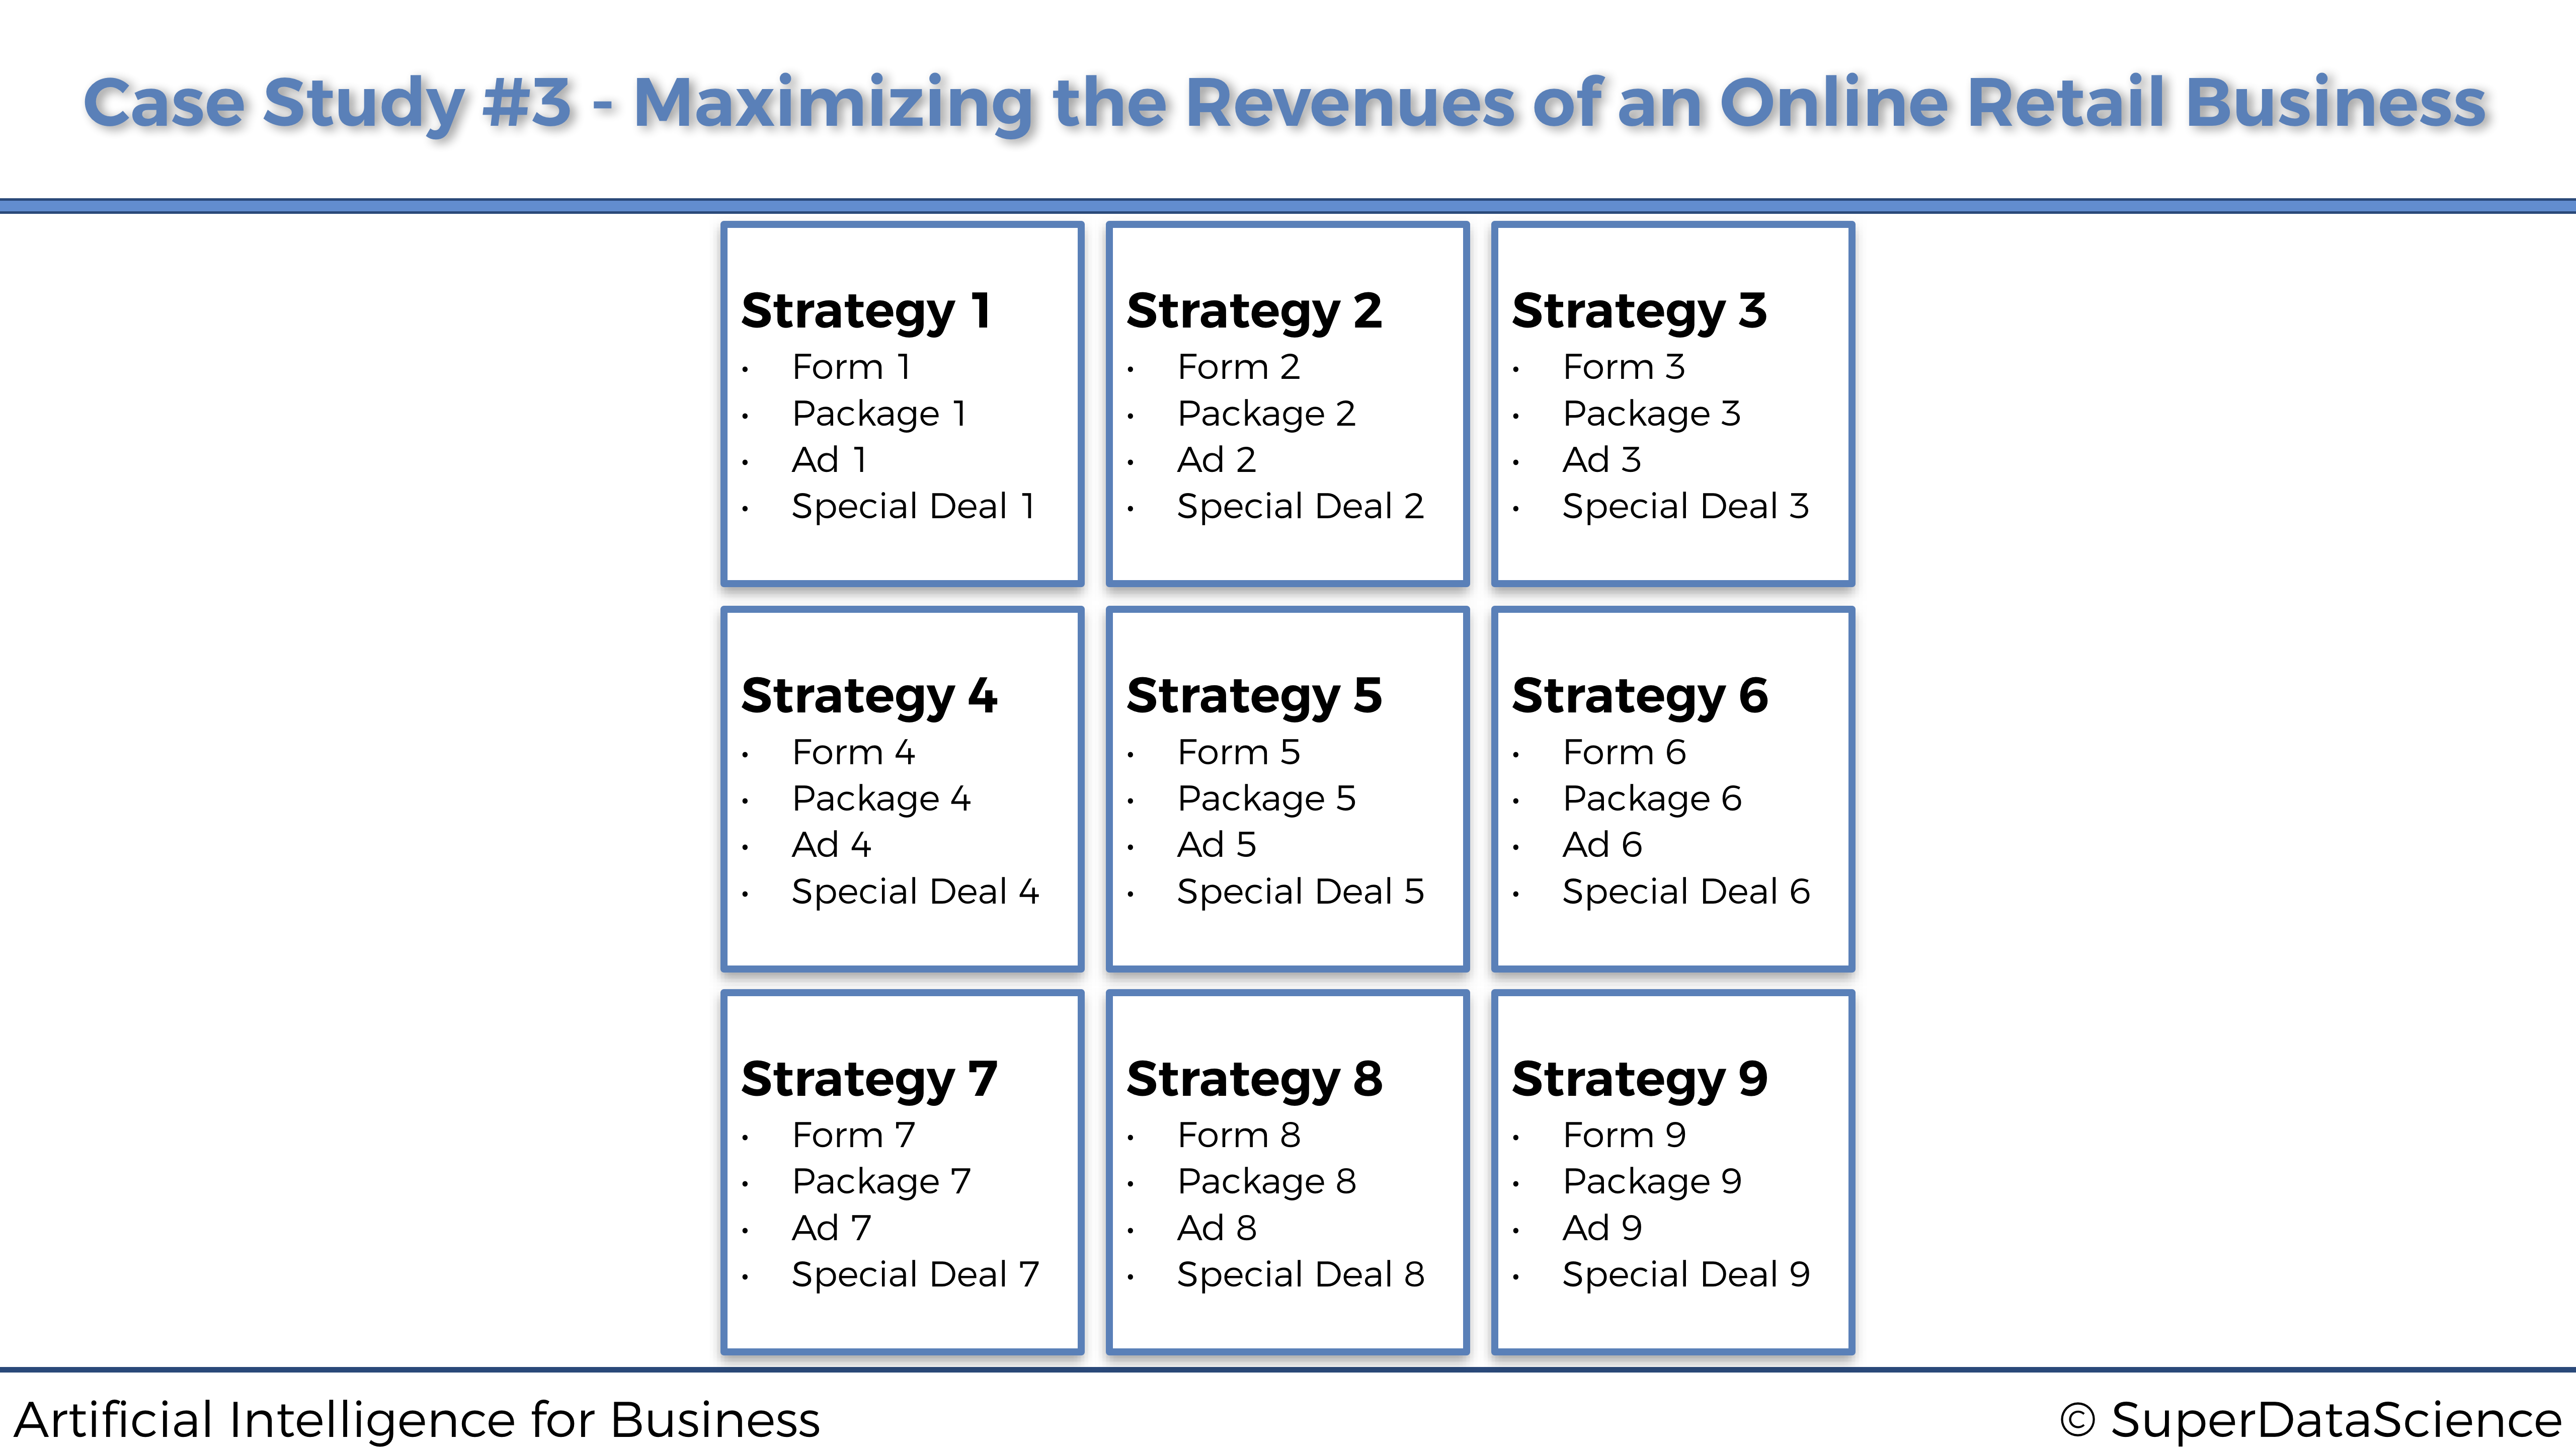
\includegraphics[scale=0.165]{Strategies_Slide.png}
        \end{center}
\end{figure}

\textbf{Simulation.}

In order to simulate this case study, we will assume these strategies have the following conversion rates:

\begin{figure}[!htbp]
        \begin{center}
            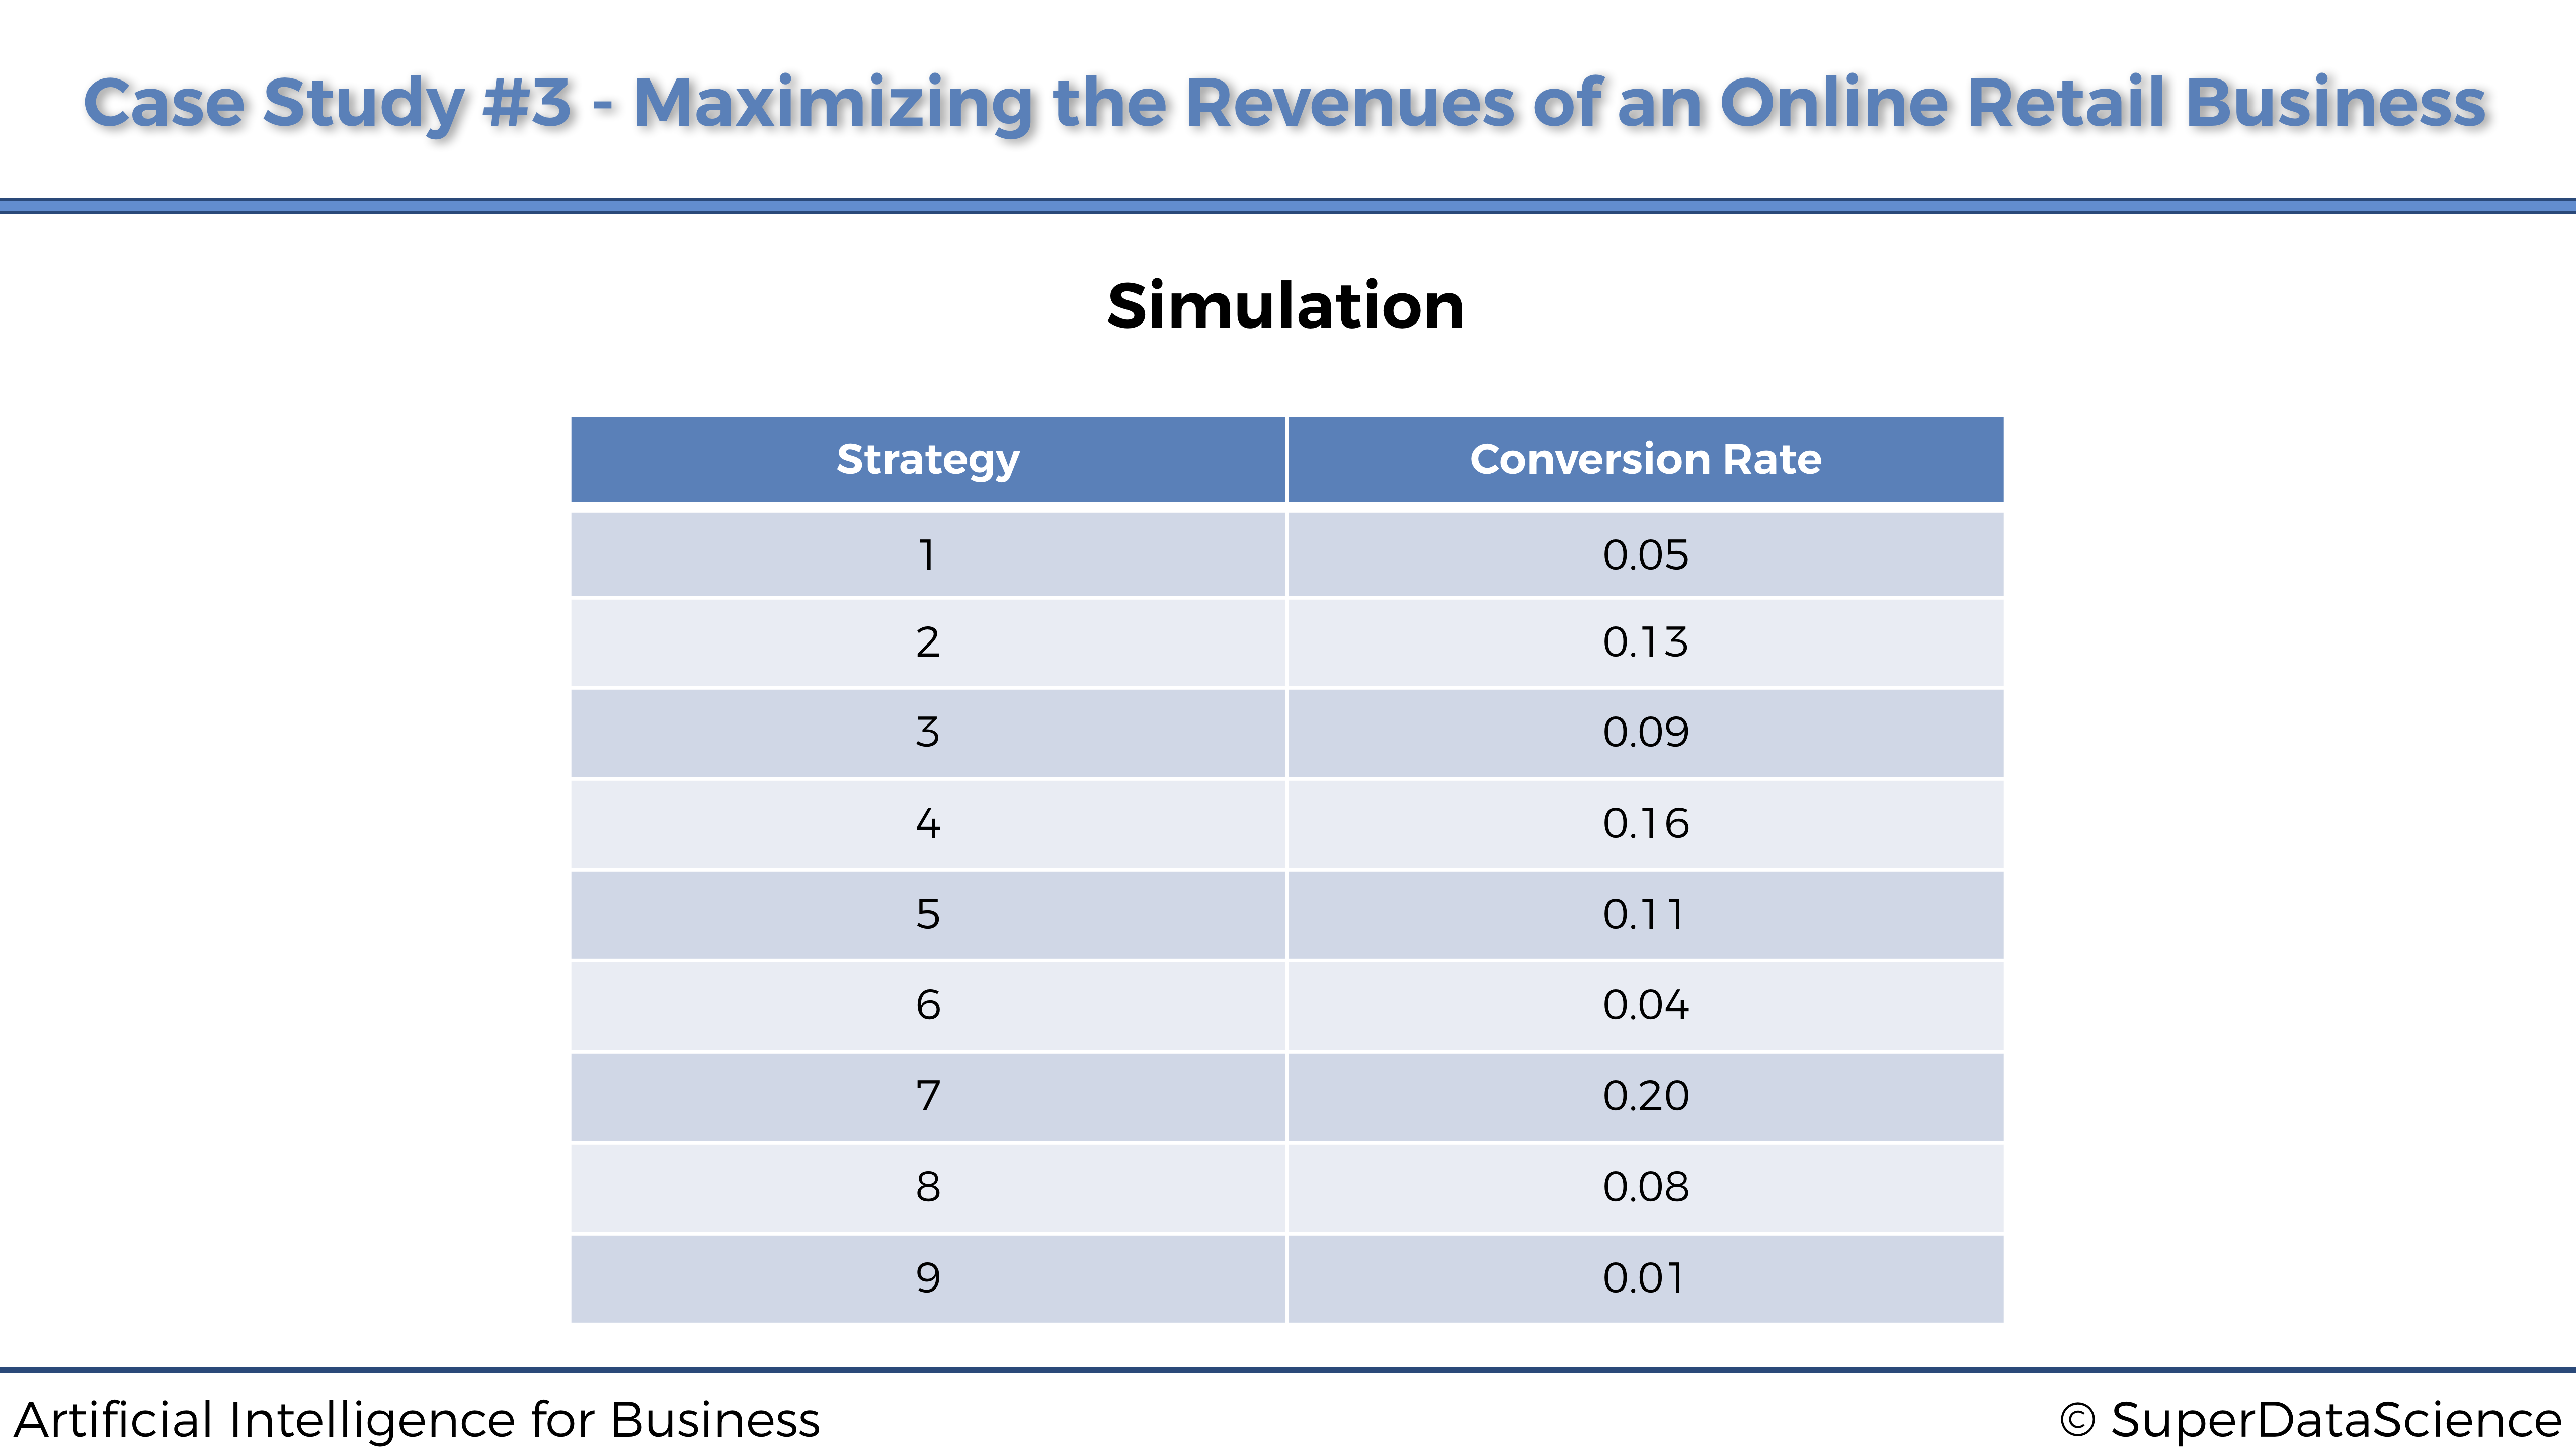
\includegraphics[scale=0.165]{Simulation_Slide.png}
        \end{center}
\end{figure}

However, please make sure to understand that in a real life situation we would have no idea of what would be these conversion rates. We only know them here for simulation purposes, just so that we can check in the end that our AI manages to figure out the best strategy, which according to the table above, is strategy number 7 (highest conversion rate).

\subsubsection{Environment to define}

Online Learning is a special branch of Artificial Intelligence, where there is not much need of defining the states and actions. Here, a state would simply be a specific customer onto whom we deploy a strategy, and the action would simply be the strategy selected. But you will see further in the AI algorithm that we don't have the states as inputs and the actions as outputs like in our two previous case studies, because this time we are not doing Q-Learning or Deep Q-Learning. Here we are doing online learning. However we do have to define the rewards, since again we will have to make a rewards matrix, where each row corresponds to a user being deployed a strategy, and each column corresponds to one of the 9 strategies. Therefore, since we will actually run this online learning experiment on 10,000 customers, this rewards matrix will have 10,000 rows and 9 columns. Then, each cell will get either a 0 if the customer doesn't subscribe to the premium plan after being approached by the selected strategy, and a 1 if the customer does subscribe after being approached by the selected strategy. And the values in the cell are exactly, the rewards.

Now a very important thing to understand is that the rewards matrix is only here for the simulation, and in real life we would have no such thing as a rewards matrix. We will just simulate 10,000 customers successively being approached by one of the 9 strategies, and thanks to the rewards matrix we will simulate the decision of the customer to subscribe yes or no to the premium plan. If the cell corresponding to a specific customer and a specific selected strategy has a 1, that will simulate a conversion by the customer to the premium plan, and if the cell has a 0, that will simulate a rejection. Here is below as an example the first rows of a simulated rewards matrix:

\begin{figure}[!htbp]
        \begin{center}
            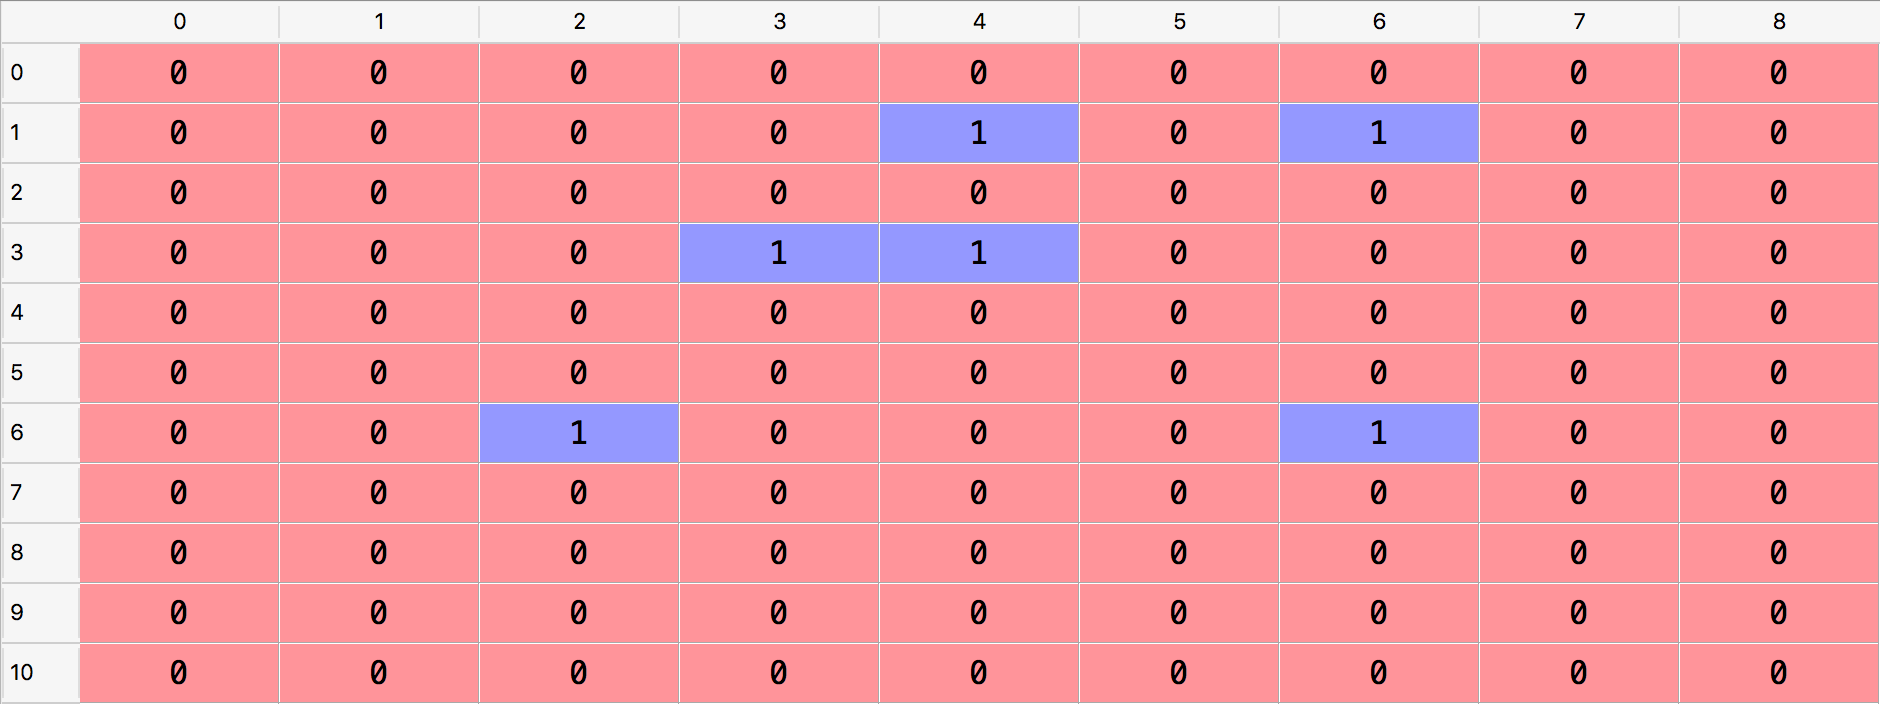
\includegraphics[scale=0.49]{Rewards_Matrix.png}
        \end{center}
\end{figure}

According to this simulation, all given in the above rewards matrix:

\begin{enumerate}
    \item The first customer (row of index 0) would not subscribe to the premium plan after being approached by any strategy.
    \item The second customer (row of index 1) would subscribe to the premium plan after being approached by strategy 5 or strategy 7 only.
    \item The third customer (row of index 2) would not subscribe to the premium plan after being approached by any strategy.
\end{enumerate}

Thompson Sampling will collect the feed-backs of whether or not each of these customers subscribe to the premium plan one after the other, and thanks to its powerful algorithm, will quickly figure out the strategy with the highest conversion rate, that is the best one to be deployed on the millions of customers, thus maximizing the company's income from this new revenue stream.

\subsection{AI Solution}

The AI solution that will figure out the best strategy is called ``Thompson Sampling''. It is by far the best model for that kind of problems in this Online Learning branch of Artificial Intelligence. To recap, each time a new customer connects to the online retail business website, that's a new round \(n\) and we select one of our 9 strategies to attempt a conversion (subscription to the premium plan). The goal is to select the best strategy at each round, over many rounds. Here is how Thompson Sampling will do that:

\textbf{For each round $n$, repeat, over 1000 rounds, the following three steps:}

\begin{enumerate}

    \item \textbf{Step 1.} For each strategy $i$, we take a random draw from the following distribution:
    \begin{equation*}
        \theta_i(n) \sim \beta(N_i^1(n)+1,N_i^0(n)+1)
    \end{equation*}
    where:
    \begin{equation*}
        \begin{cases}
            \textrm{$N_i^1(n)$ is the number of times the strategy $i$ has received a 1 reward up to round $n$,} \\
            \textrm{$N_i^0(n)$ is the number of times the strategy $i$ has received a 0 reward up to round $n$.}
        \end{cases}
    \end{equation*}
    
    \item \textbf{Step 2.} We select the strategy $s(n)$ that has the highest $\theta_i(n)$:
    \begin{equation*}
        s(n) = \underset{i\in\{1,...,9\}}{\textrm{argmax}}(\theta_i(n))
    \end{equation*}
    
    \item \textbf{Step 3.} We update $N_{s(n)}^1(n)$ and $N_{s(n)}^0(n)$ according to the following conditions:
    \begin{itemize}
        \item If the strategy selected $s(n)$ received a 1 reward:
        \begin{equation*}
            N_{s(n)}^1(n) := N_{s(n)}^1(n) + 1
        \end{equation*}
        \item If the strategy selected $s(n)$ received a 0 reward:
        \begin{equation*}
            N_{s(n)}^0(n) := N_{s(n)}^0(n) + 1
        \end{equation*}
    \end{itemize}

\end{enumerate}

\textbf{Intuition.} Each strategy has its own beta distribution. Over the rounds, the beta distribution of the strategy with the highest conversion rate will be progressively shifted to the right, and the beta distributions of the strategies with lower conversion rates will be progressively shifted to the left (Steps 1 and 3). Therefore, because of Step 2, the strategy with the highest conversion rate will be more and more selected. Below is a graph displaying three beta distributions of three strategies, that will help you visualize this:

\begin{figure}[!htbp]
        \begin{center}
            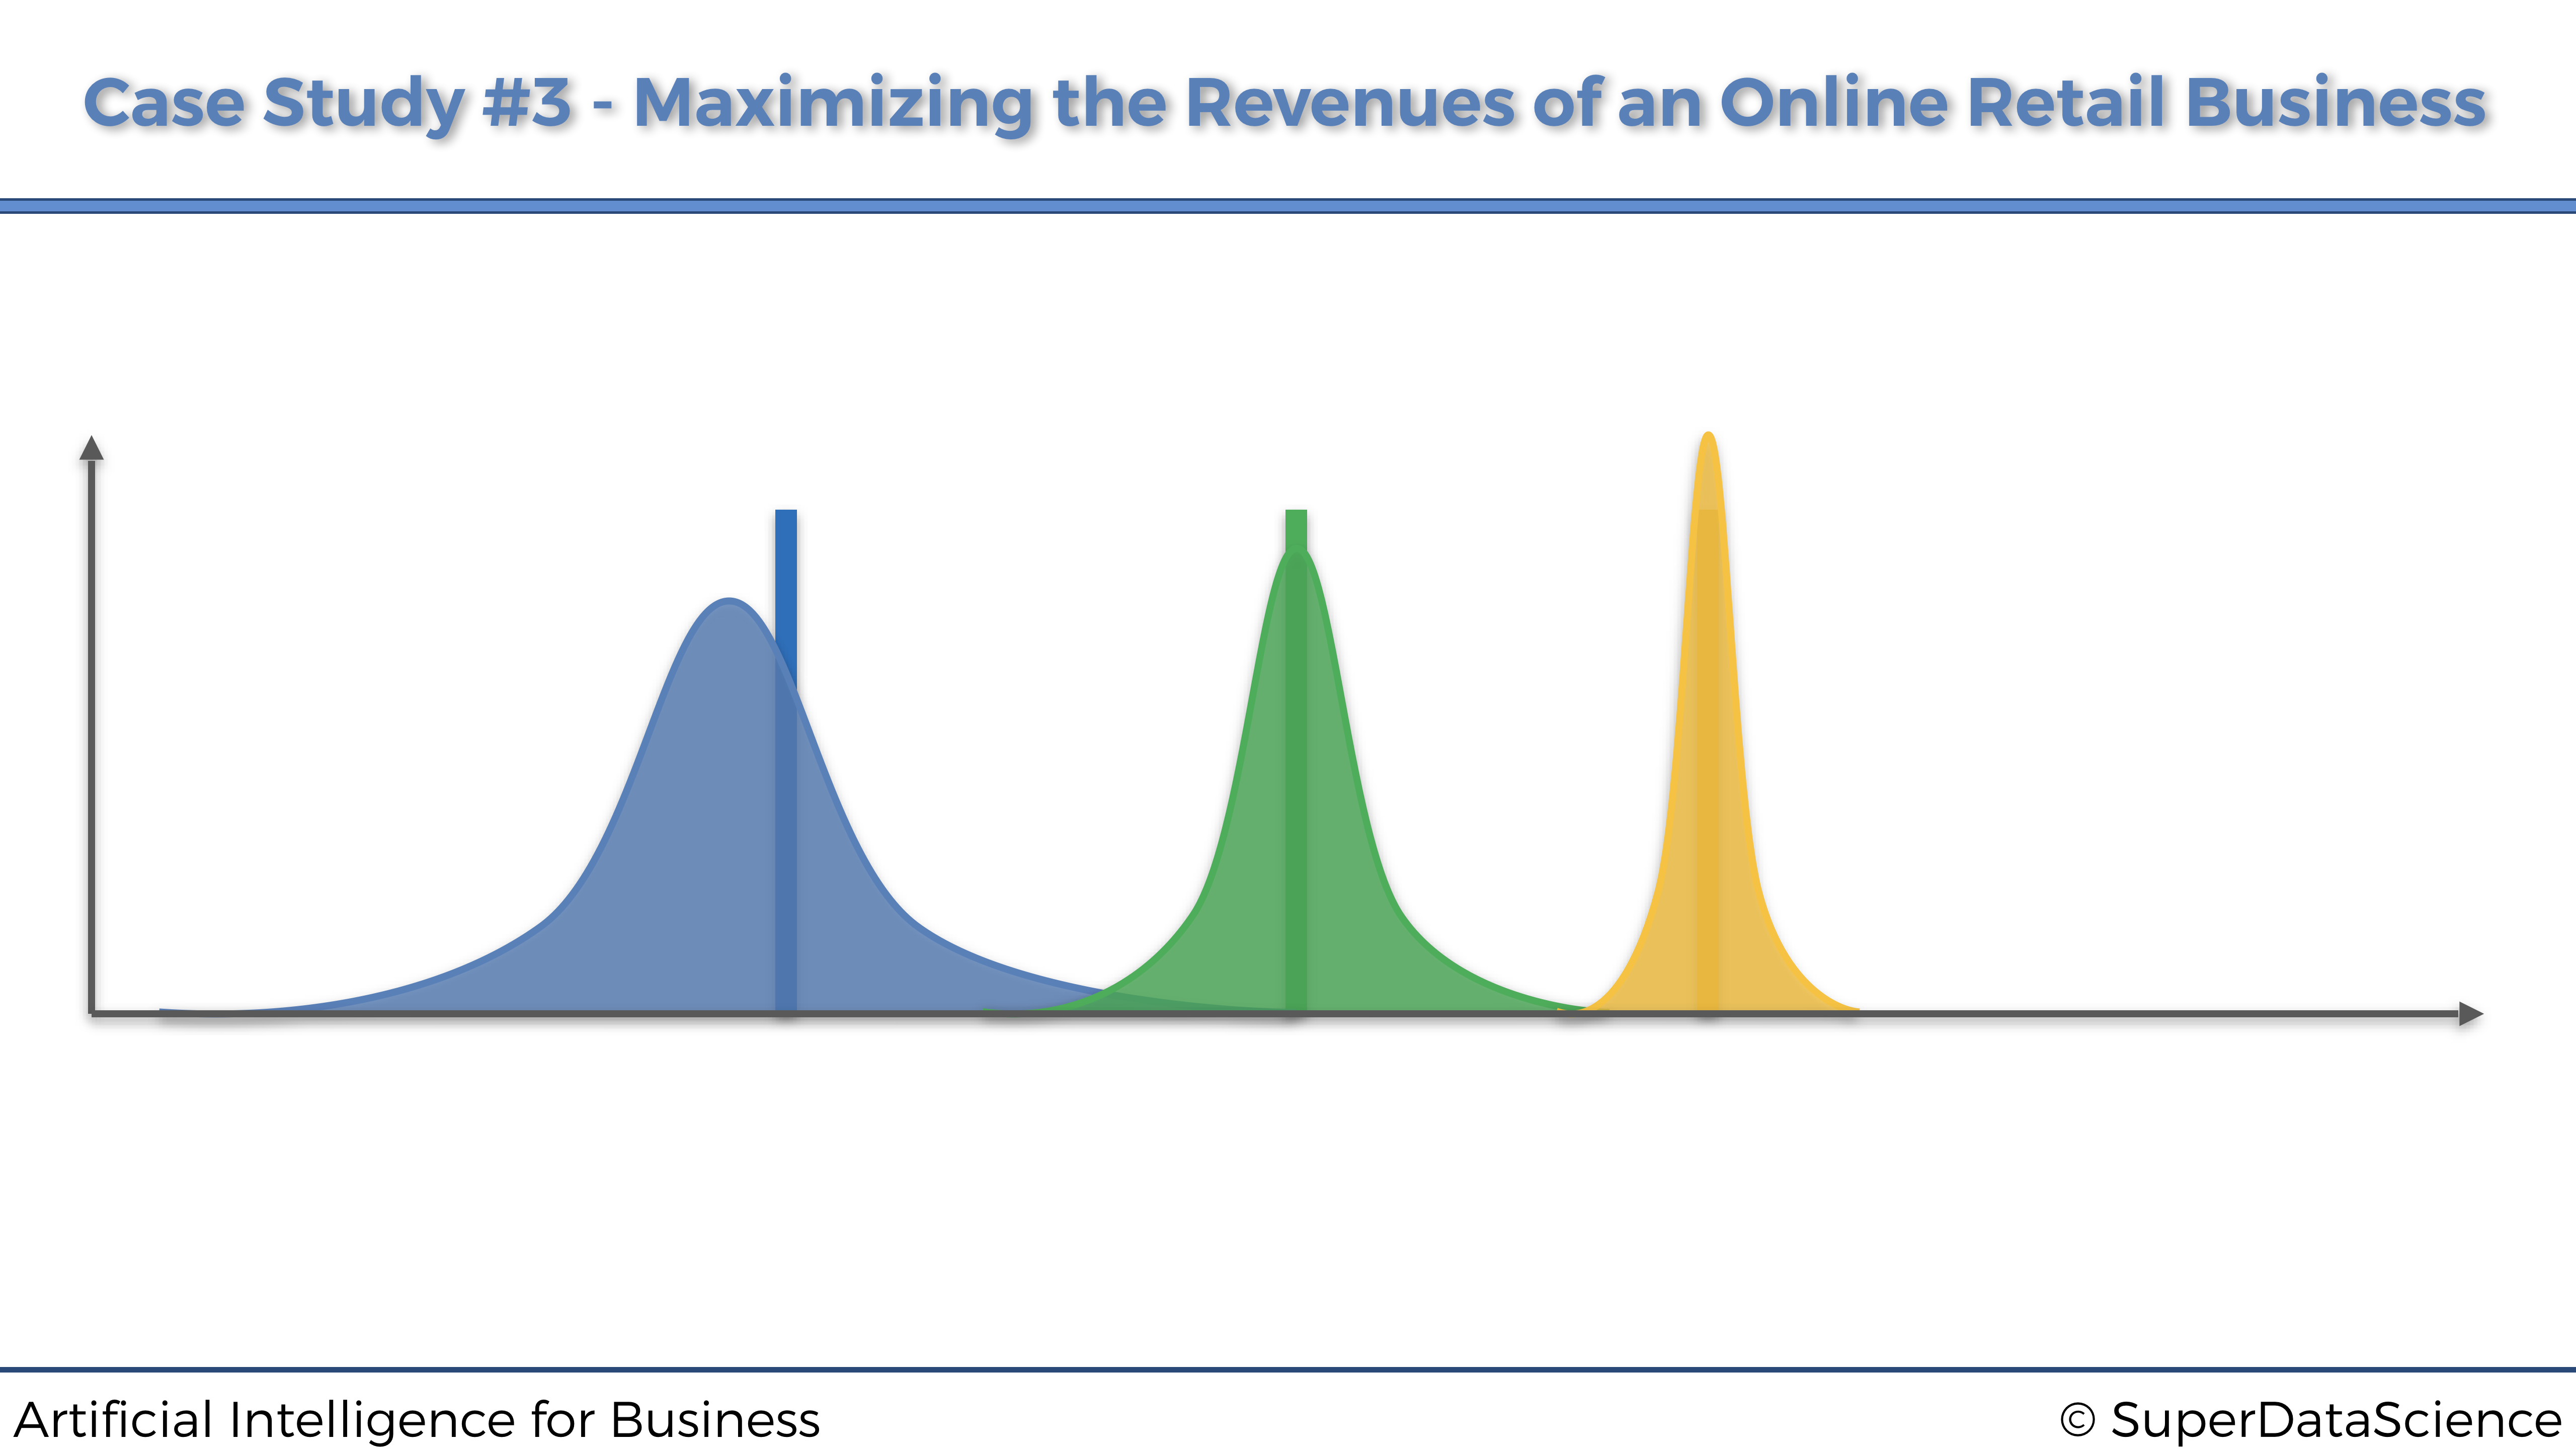
\includegraphics[scale=0.1]{Beta_Distribution_Slide.png}
        \end{center}
\end{figure}

\newpage

\subsection{Implementation}

Let's provide the whole implementation of Thompson Sampling for this specific case study, following the same simulation given above.

While implementing Thompson Sampling, we will also implement the Random Selection algorithm, which will simply select a random strategy at each round. This will be our benchmark to evaluate the performance of our Thompson Sampling model. Of course, Thompson Sampling and the Random Selection algorithm will be competing on the same simulation, that is on the same rewards matrix. And in the end, after the whole simulation is done, we will assess the performance of Thompson Sampling by computing the relative return, defined by the following formula:

\begin{equation*}
    \textrm{Relative Return} = \frac{\textrm{(Total Reward of Thompson Sampling)} - (\textrm{Total Reward of Random Selection})}{\textrm{Total Reward of Random Selection}} \times 100
\end{equation*}

We will also plot the histogram of selected ads, just to check that the strategy with the highest conversion rate (Strategy 7) was the one selected the most.

So if you are ready, here we go:

First, we import the required libraries and we set the parameters (\(N = 10000\) customers and \(d = 9\) strategies):

\begin{lstlisting}
# Artificial Intelligence for Business
# Maximizing the Revenues of an Online Retail Business with Thompson Sampling

# Importing the libraries
import numpy as np
import matplotlib.pyplot as plt
import random

# Setting the parameters
N = 10000
d = 9
\end{lstlisting}

Then, we create the simulation, by building the rewards matrix of 10000 rows corresponding to the customers, and 9 columns corresponding to the strategies. At each round and for each strategy, we draw a random number between 0 and 1, and if this random number is lower than the conversion rate of the strategy, the reward will be 1. Otherwise, it will be 0. That way we simulate the conversion rates listed above for our 9 strategies:

\begin{lstlisting}
# Creating the simulation
# conversion_rates = [0.1,0.2,0.3,0.4,0.5,0.6,0.7,0.8,0.9]
conversion_rates = [0.05,0.13,0.09,0.16,0.11,0.04,0.20,0.08,0.01]
X = np.array(np.zeros([N,d]))
for i in range(N):
    for j in range(d):
        if np.random.rand() <= conversion_rates[j]:
            X[i,j] = 1
\end{lstlisting}

Then, we will loop over the 10000 rows (or rounds) of this rewards matrix, and at each round we will get two separate strategy selections: one from the Random Selection algorithm, and one from Thompson Sampling. We keep track of the strategies selected by each of these two algorithms, and we compute the total reward accumulated over the rounds by each of them. Thompson Sampling is implemented following exactly the Steps 1, 2 and 3 provided above:

\begin{lstlisting}
# Implementing a Random Strategy and Thompson Sampling
strategies_selected_rs = []
strategies_selected_ts = []
total_reward_rs = 0
total_reward_ts = 0
numbers_of_rewards_1 = [0] * d
numbers_of_rewards_0 = [0] * d
for n in range(0, N):
    # Random Strategy
    strategy_rs = random.randrange(d)
    strategies_selected_rs.append(strategy_rs)
    reward_rs = X[n, strategy_rs]
    total_reward_rs = total_reward_rs + reward_rs
    # Thompson Sampling
    strategy_ts = 0
    max_random = 0
    for i in range(0, d):
        random_beta = random.betavariate(numbers_of_rewards_1[i] + 1,
                                         numbers_of_rewards_0[i] + 1)
        if random_beta > max_random:
            max_random = random_beta
            strategy_ts = i
    reward_ts = X[n, strategy_ts]
    if reward_ts == 1:
        numbers_of_rewards_1[strategy_ts] = numbers_of_rewards_1[strategy_ts] + 1
    else:
        numbers_of_rewards_0[strategy_ts] = numbers_of_rewards_0[strategy_ts] + 1
    strategies_selected_ts.append(strategy_ts)
    total_reward_ts = total_reward_ts + reward_ts
\end{lstlisting}

Then we compute the final score, which is the relative return of Thompson Sampling with respect to our benchmark that is the Random Selection:

\begin{lstlisting}
# Computing the Relative Return
relative_return = (total_reward_ts - total_reward_rs) / total_reward_rs * 100
print("Relative Return: {:.0f} %".format(relative_return))
\end{lstlisting}

And buckle up, by executing this code we obtain a final relative return, of\ldots{}:

\begin{equation*}
    \textrm{Relative Return} = 91 \ \% \ !
\end{equation*}

In other words, Thompson Sampling almost doubled the performance of our Random Selection benchmark.

\newpage

And finally, we plot the Histogram of the selected strategies, to check that indeed Strategy 7 (of index 6) was the one most selected, since it is the one having the highest conversion rate:

\begin{lstlisting}
# Plotting the Histogram of Selections
plt.hist(strategies_selected_ts)
plt.title('Histogram of Selections')
plt.xlabel('Strategy')
plt.ylabel('Number of times the strategy was selected')
plt.show()
\end{lstlisting}

By executing this final code, we obtain the following histogram:

\begin{figure}[!htbp]
        \begin{center}
            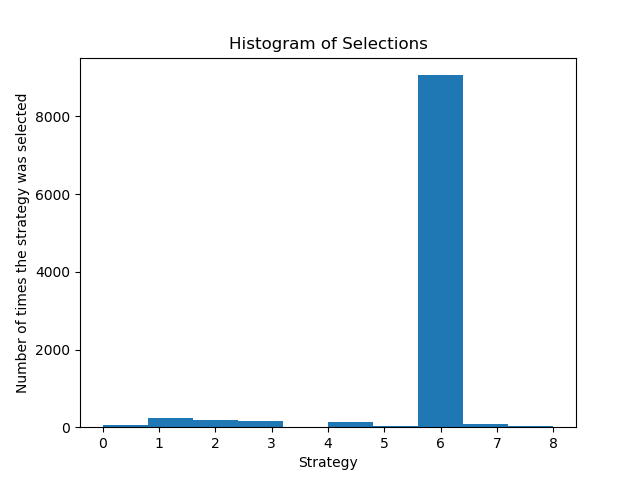
\includegraphics[scale=0.8]{Histogram.png}
        \end{center}
\end{figure}

And indeed, it is well the strategy of index 6, that is Strategy 7, that was, by far, selected the most. Thompson Sampling was quickly able to identify it. And in fact, if we re-run the same code but with only 1000 customers, we realize that Thompson Sampling is still able to identify Strategy 7 as the best one.

Accordingly, Thompson Sampling surely did an amazing job for this Online Retail Business. Because not only it was able to identify the best strategy quickly in a few number of rounds, that is with a few customers, which saved a lot on the advertising and operating related costs. But also because of course, it was able to clearly figure out the strategy with the highest conversion rate. And indeed, if this Online Retail Business has 100 million customers, and if the premium plan has a price of \$ 100 per year, then deploying this best strategy that has a conversion rate of 20 \% would lead to generate an extra revenue of\ldots{}:

\begin{equation*}
    \textrm{Extra Revenues generated} = 100000000 \times 0.2 \times 100 = \textrm{\$ $2$ Billion !!}
\end{equation*}

In other words, Thompson Sampling clearly and quickly maximized the revenues of this online retail business, while also saving a lot on the costs, therefore maximizing as well the profitability of the business.

\textbf{Regret Curve.}

The regret curve of a model (Random Strategy or Thompson Sampling) is the plot of the difference between the best strategy and the deployed model, with respect to the rounds.

The best strategy is computed by simply getting, at each round, the maximum of the accumulated rewards over all the different strategies. Therefore in our implementation, we will get the best strategy the following way:

\begin{lstlisting}
rewards_strategies = [0] * d
for n in range(0, N):
    # Best Strategy
    for i in range(0, d):
        rewards_strategies[i] = rewards_strategies[i] + X[n, i]
    total_reward_bs = max(rewards_strategies)
\end{lstlisting}

Then, the regret of Thompson Sampling is simply computed as the difference between the best strategy and the Thompson Sampling model:

\begin{lstlisting}
# Regret of Thompson Sampling
strategies_selected_ts = []
total_reward_ts = 0
total_reward_bs = 0
numbers_of_rewards_1 = [0] * d
numbers_of_rewards_0 = [0] * d
rewards_strategies = [0] * d
regret = []
for n in range(0, N):
    # Thompson Sampling
    strategy_ts = 0
    max_random = 0
    for i in range(0, d):
        random_beta = random.betavariate(numbers_of_rewards_1[i] + 1,
                                         numbers_of_rewards_0[i] + 1)
        if random_beta > max_random:
            max_random = random_beta
            strategy_ts = i
    reward_ts = X[n, strategy_ts]
    if reward_ts == 1:
        numbers_of_rewards_1[strategy_ts] = numbers_of_rewards_1[strategy_ts] + 1
    else:
        numbers_of_rewards_0[strategy_ts] = numbers_of_rewards_0[strategy_ts] + 1
    strategies_selected_ts.append(strategy_ts)
    total_reward_ts = total_reward_ts + reward_ts
    # Best Strategy
    for i in range(0, d):
        rewards_strategies[i] = rewards_strategies[i] + X[n, i]
    total_reward_bs = max(rewards_strategies)
    # Regret
    regret.append(total_reward_bs - total_reward_ts)
\end{lstlisting}

And same, the regret of the Random Strategy is simply computed as the difference between the best strategy and the random selection algorithm:

\begin{lstlisting}
# Regret of the Random Strategy
strategies_selected_rs = []
total_reward_rs = 0
total_reward_bs = 0
numbers_of_rewards_1 = [0] * d
numbers_of_rewards_0 = [0] * d
rewards_strategies = [0] * d
regret = []
for n in range(0, N):
    # Random Strategy
    strategy_rs = random.randrange(d)
    strategies_selected_rs.append(strategy_rs)
    reward_rs = X[n, strategy_rs]
    total_reward_rs = total_reward_rs + reward_rs
    # Best Strategy
    for i in range(0, d):
        rewards_strategies[i] = rewards_strategies[i] + X[n, i]
    total_reward_bs = max(rewards_strategies)
    # Regret
    regret.append(total_reward_bs - total_reward_rs)
\end{lstlisting}

And finally of course, we plot the regret over the rounds with this simple code (we don't have to specify the x-coordinates in the plt.plot() function because the rounds are already indexes from 0 to N):

\begin{lstlisting}
# Plotting the Regret Curve
plt.plot(regret)
plt.title('Regret Curve')
plt.xlabel('Round')
plt.ylabel('Regret')
plt.show()
\end{lstlisting}

Let's look at the results in the next page, for both the Random Strategy and Thompson Sampling.

\newpage

If we plot the Regret Curve of the Random Strategy, we thus obtain the following:

\begin{figure}[!htbp]
        \begin{center}
            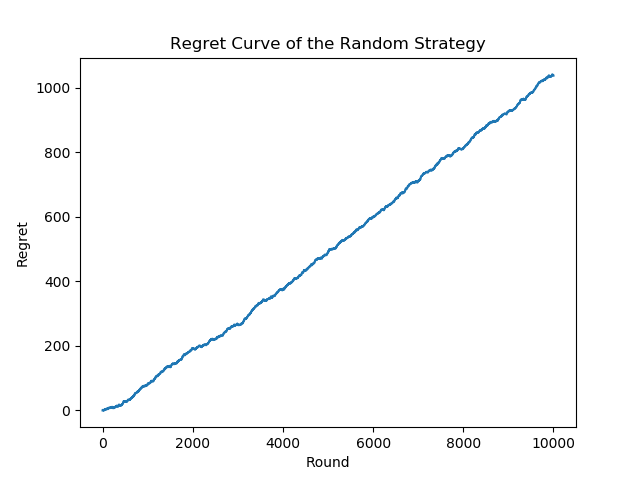
\includegraphics[scale=1]{Regret_Curve_Random_Strategy.png}
        \end{center}
\end{figure}

And of course, we observe absolutely no convergence of the Random Strategy towards the Best Strategy.

\newpage

However if now we plot the Regret Curve of the Thompson Sampling model, we get the following beautiful curve:

\begin{figure}[!htbp]
        \begin{center}
            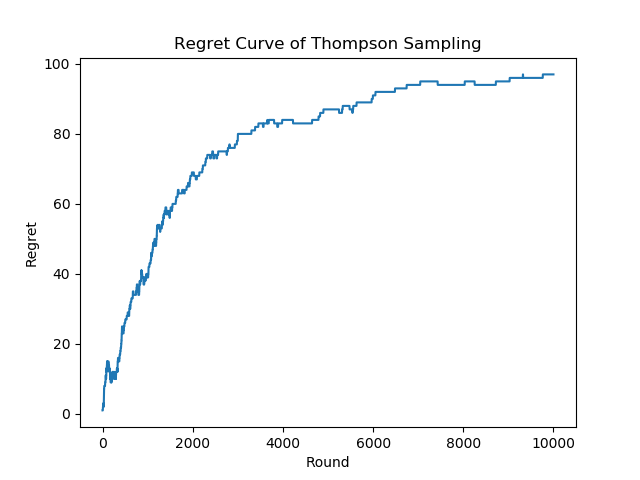
\includegraphics[scale=1]{Regret_Curve_Thompson_Sampling.png}
        \end{center}
\end{figure}

And obviously, Thompson Sampling is converging very well towards the best strategy.

\newpage

Eventually, here is the final code including that Regret Curve of Thompson Sampling:

\begin{lstlisting}
# Thompson Sampling

# Importing the libraries
import numpy as np
import matplotlib.pyplot as plt
import random

# Setting the parameters
N = 10000
d = 9

# Creating the simulation
# conversion_rates = [0.1,0.2,0.3,0.4,0.5,0.6,0.7,0.8,0.9]
conversion_rates = [0.05,0.13,0.09,0.16,0.11,0.04,0.20,0.08,0.01]
X = np.array(np.zeros([N,d]))
for i in range(N):
    for j in range(d):
        if np.random.rand() <= conversion_rates[j]:
            X[i,j] = 1

# Implementing a Random Strategy and Thompson Sampling with Regret Curve
strategies_selected_rs = []
strategies_selected_ts = []
total_reward_rs = 0
total_reward_ts = 0
total_reward_bs = 0
numbers_of_rewards_1 = [0] * d
numbers_of_rewards_0 = [0] * d
rewards_strategies = [0] * d
regret = []
for n in range(0, N):
    # Random Strategy
    strategy_rs = random.randrange(d)
    strategies_selected_rs.append(strategy_rs)
    reward_rs = X[n, strategy_rs]
    total_reward_rs = total_reward_rs + reward_rs
    # Thompson Sampling
    strategy_ts = 0
    max_random = 0
    for i in range(0, d):
        random_beta = random.betavariate(numbers_of_rewards_1[i] + 1,
                                         numbers_of_rewards_0[i] + 1)
        if random_beta > max_random:
            max_random = random_beta
            strategy_ts = i
    reward_ts = X[n, strategy_ts]
    if reward_ts == 1:
        numbers_of_rewards_1[strategy_ts] = numbers_of_rewards_1[strategy_ts] + 1
    else:
        numbers_of_rewards_0[strategy_ts] = numbers_of_rewards_0[strategy_ts] + 1
    strategies_selected_ts.append(strategy_ts)
    total_reward_ts = total_reward_ts + reward_ts
    # Best Strategy
    for i in range(0, d):
        rewards_strategies[i] = rewards_strategies[i] + X[n, i]
    total_reward_bs = max(rewards_strategies)
    # Regret
    regret.append(total_reward_bs - total_reward_ts)

# Computing the Absolute and Relative Return
absolute_return = total_reward_ts - total_reward_rs
relative_return = (total_reward_ts - total_reward_rs) / total_reward_rs * 100
print("Absolute Return: {:.0f} $".format(absolute_return))
print("Relative Return: {:.0f} %".format(relative_return))

# Plotting the Histogram of Selections
plt.hist(strategies_selected_ts)
plt.title('Histogram of Selections')
plt.xlabel('Strategy')
plt.ylabel('Number of times the strategy was selected')
plt.show()
plt.close()

# Plotting the Regret Curve
plt.plot(regret)
plt.title('Regret Curve')
plt.xlabel('Round')
plt.ylabel('Regret')
plt.show()

\end{lstlisting}

\hypertarget{conclusion}{%
\chapter*{Conclusion}\label{conclusion}}
\addcontentsline{toc}{chapter}{Conclusion}

Thank you so much again for joining this course, and congratulations for completing it! We highly recommend that you keep this book close to you whenever you are building an AI to solve a business problem. Or at least, try to keep the general AI Framework. On our side, it was our pleasure making this course, and writing this book. Don't hesitate to leave a review in the course if you wish. Until then, enjoy AI for Business!

\hypertarget{annex-1-artificial-neural-networks}{%
\chapter{Annex 1: Artificial Neural Networks}\label{annex-1-artificial-neural-networks}}

In this annex part you will find all the intuition and theory of Artificial Neural Networks, which are at the heart of the Deep Q-Learning model we build in Part 2 - Minimizing the Costs. Here is the plan of attack to study Artificial Neural Networks:

\begin{enumerate}
    \item The Neuron
    \item The Activation Function
    \item How do Neural Networks work?
    \item How do Neural Networks learn?
    \item Forward-Propagation and Back-Propagation
    \item Gradient Descent
    \item Batch Gradient Descent and Stochastic Gradient Descent
\end{enumerate}

\subsection{The Neuron}

The neuron is the basic building block of Artificial Neural Networks. In the images below are actual real life neurons which have been smeared onto a glass, colored a little bit and observed through a microscope:

\begin{figure}[!htbp]
        \begin{center}
            \includegraphics[scale=0.18]{ANN_1.png}
        \end{center}
\end{figure}

As we can see, they have the structure of a body with lots of different branches coming out of them. But the question is: How can we recreate that in a machine? Indeed, we really need to recreate it in a machine since the whole purpose of Deep Learning is to mimic how the human brain works, in the hope that by doing so we are going to create something amazing: a powerful infrastructure for machines to be able to learn.

Why do we hope for that? Because the human brain just happens to be one of the most powerful learning tools on the planet. So we just hope that if we recreate it then we will have something as awesome as that. So our challenge right now, that is our very first step to creating artificial neural networks, is to recreate a neuron.

So how do we do it? Well, first of all let's have a closer look at what a neuron actually is. The image below was first created by a Spanish neuroscientist and Chagga Ramon Yi Kajal in 1899:

\begin{figure}[!htbp]
        \begin{center}
            \includegraphics[scale=0.16]{ANN_2.png}
        \end{center}
\end{figure}

This neuroscientist dyed in neurons in actual brain tissue, and looked at them under a microscope. While he was looking at them he actually drew what he saw, which is exactly what we see on the above image. Today technology has advanced quite a lot allowing us to see neurons much closer in more detail so that we can actually draw what it looks like diagrammatically.

\begin{figure}[!htbp]
        \begin{center}
            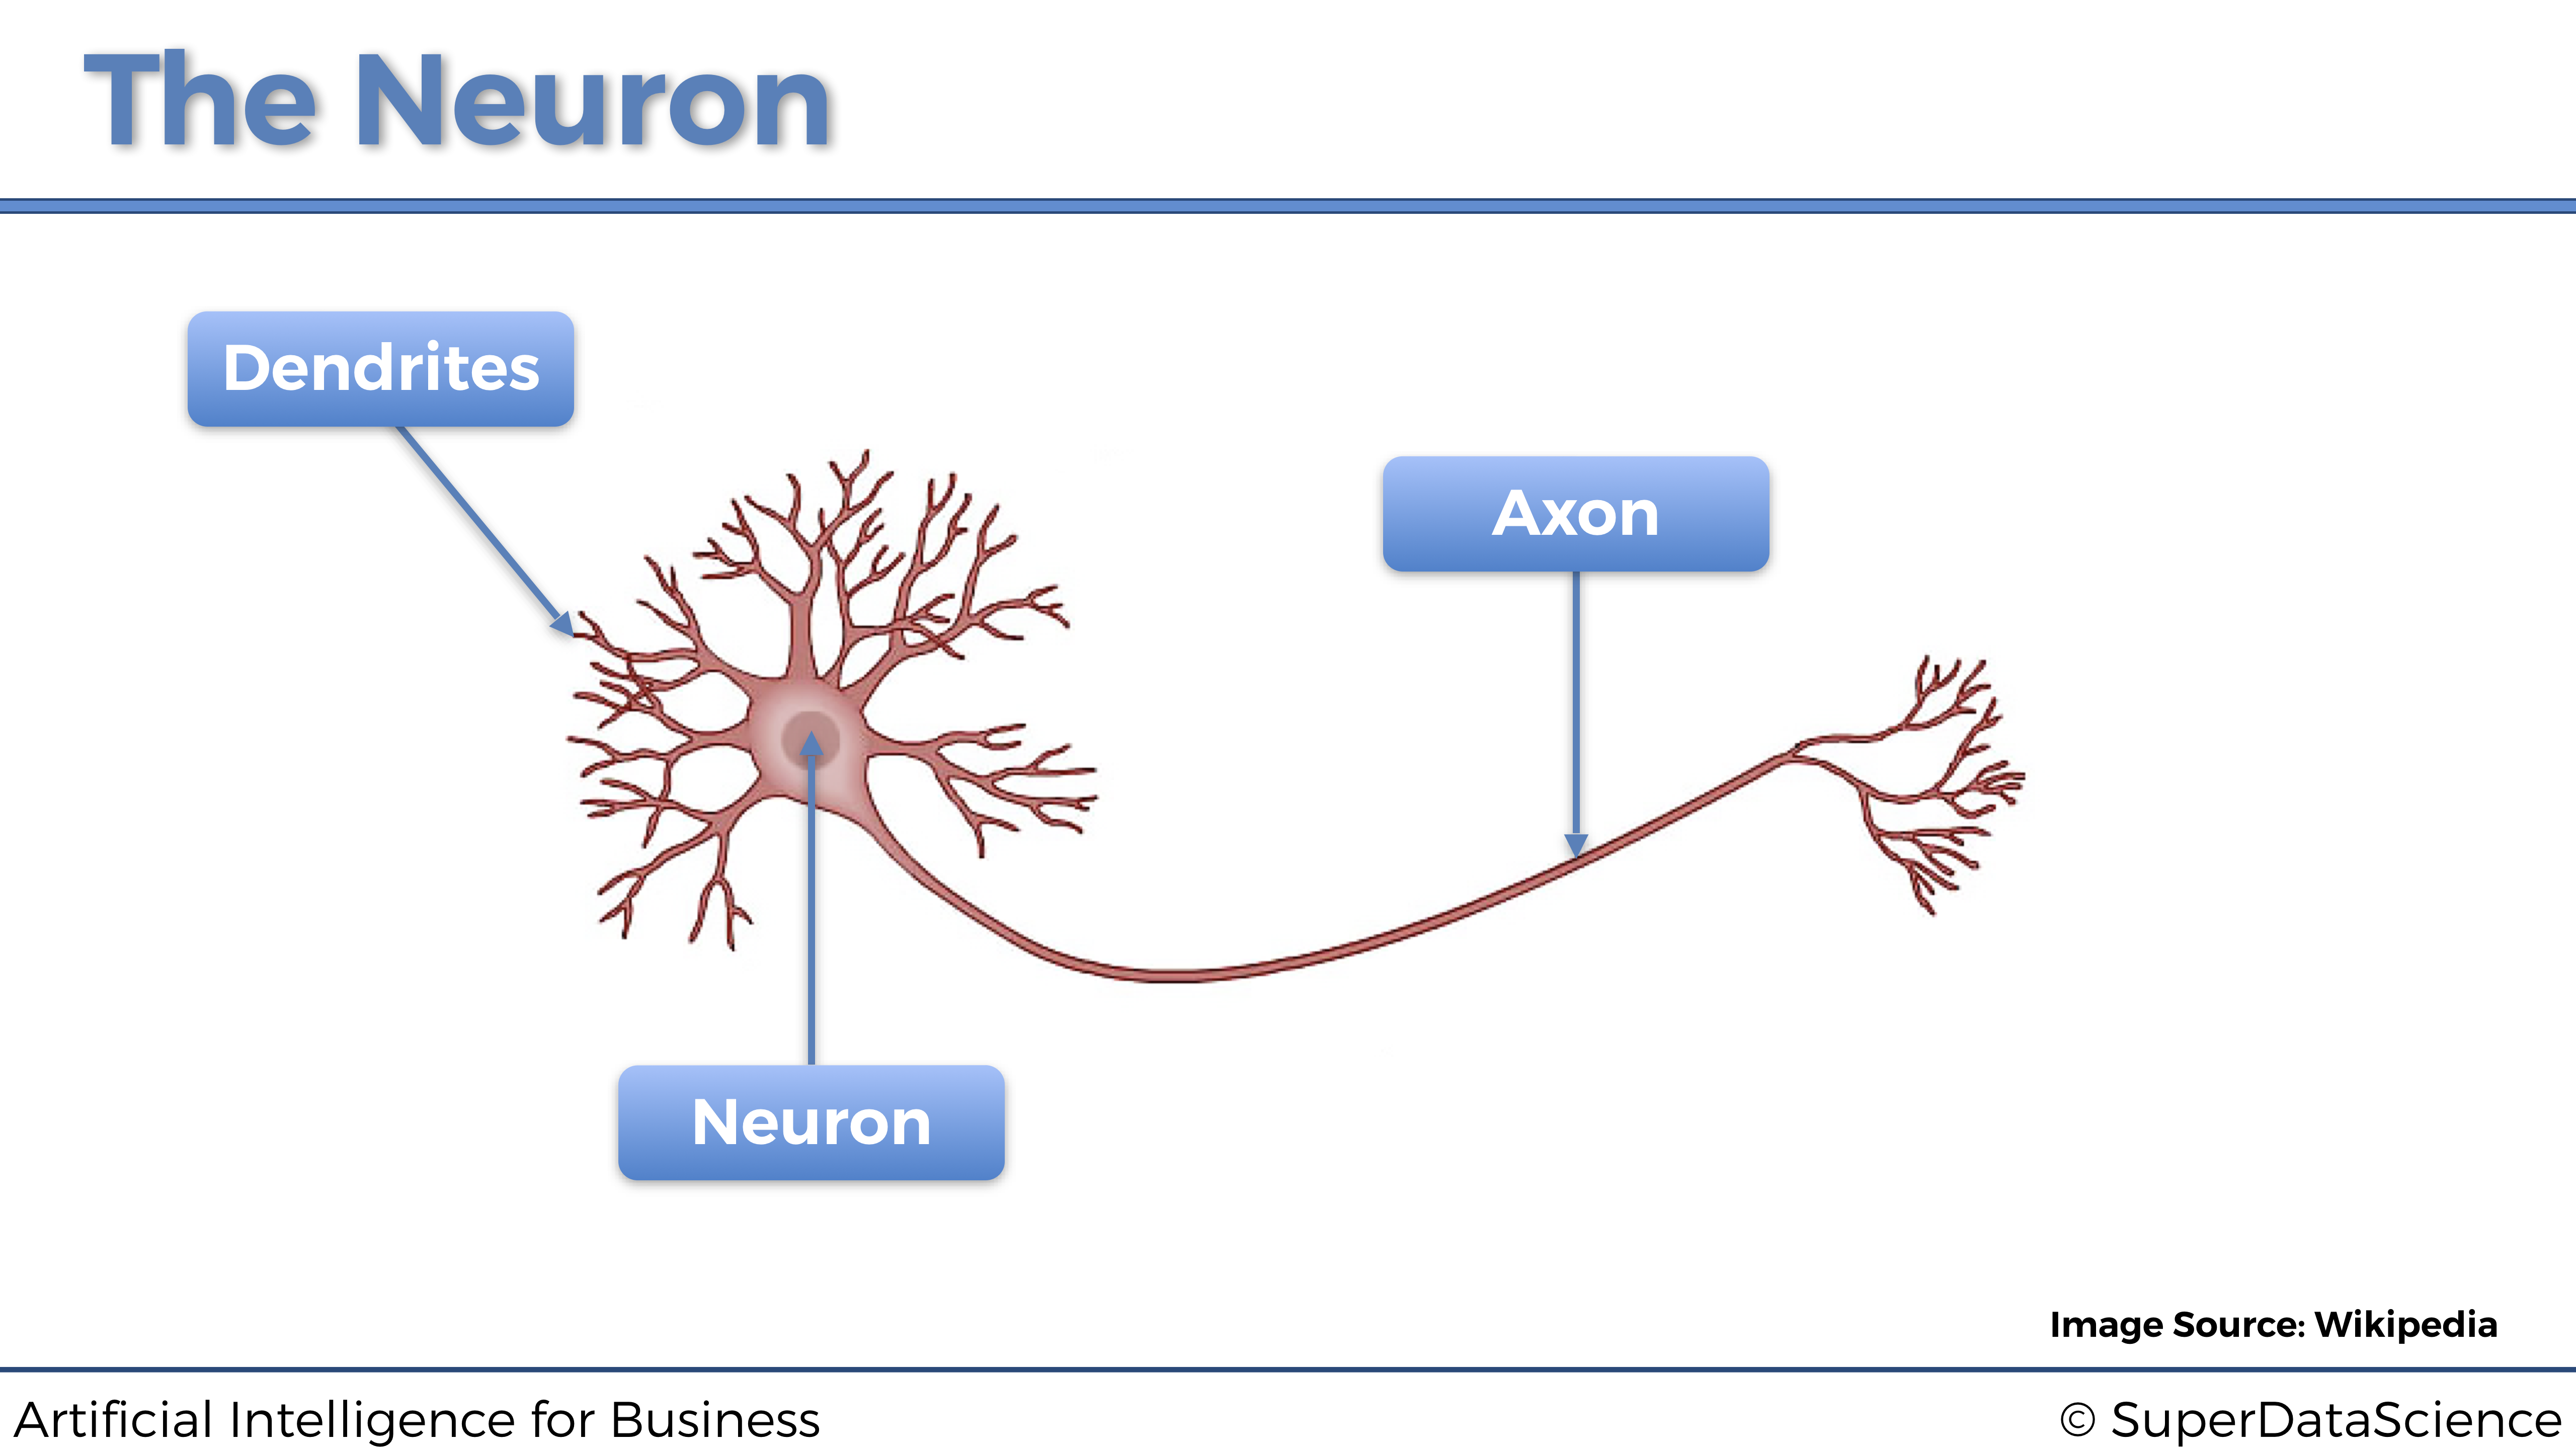
\includegraphics[scale=0.16]{ANN_3.png}
        \end{center}
\end{figure}

Above is a neuron. This neuron exchanges signals between its neighbour neurons. The dendrites are the receivers of the signal and the axon is the transmitter of the signal. Here is an image of how it all works conceptually:

\begin{figure}[!htbp]
        \begin{center}
            \includegraphics[scale=0.16]{ANN_4.png}
        \end{center}
\end{figure}

We can see that the dendrites of the neuron are connected to the axons of other neurons above it. Then the signal travels down its axon and passes on to the dendrites of the next neuron. That is how they are connected and how a neuron works. Thus now is the time to move from neuroscience to technology.

Here is how a neuron is represented inside an Artificial Neural Network:

\begin{figure}[!htbp]
        \begin{center}
            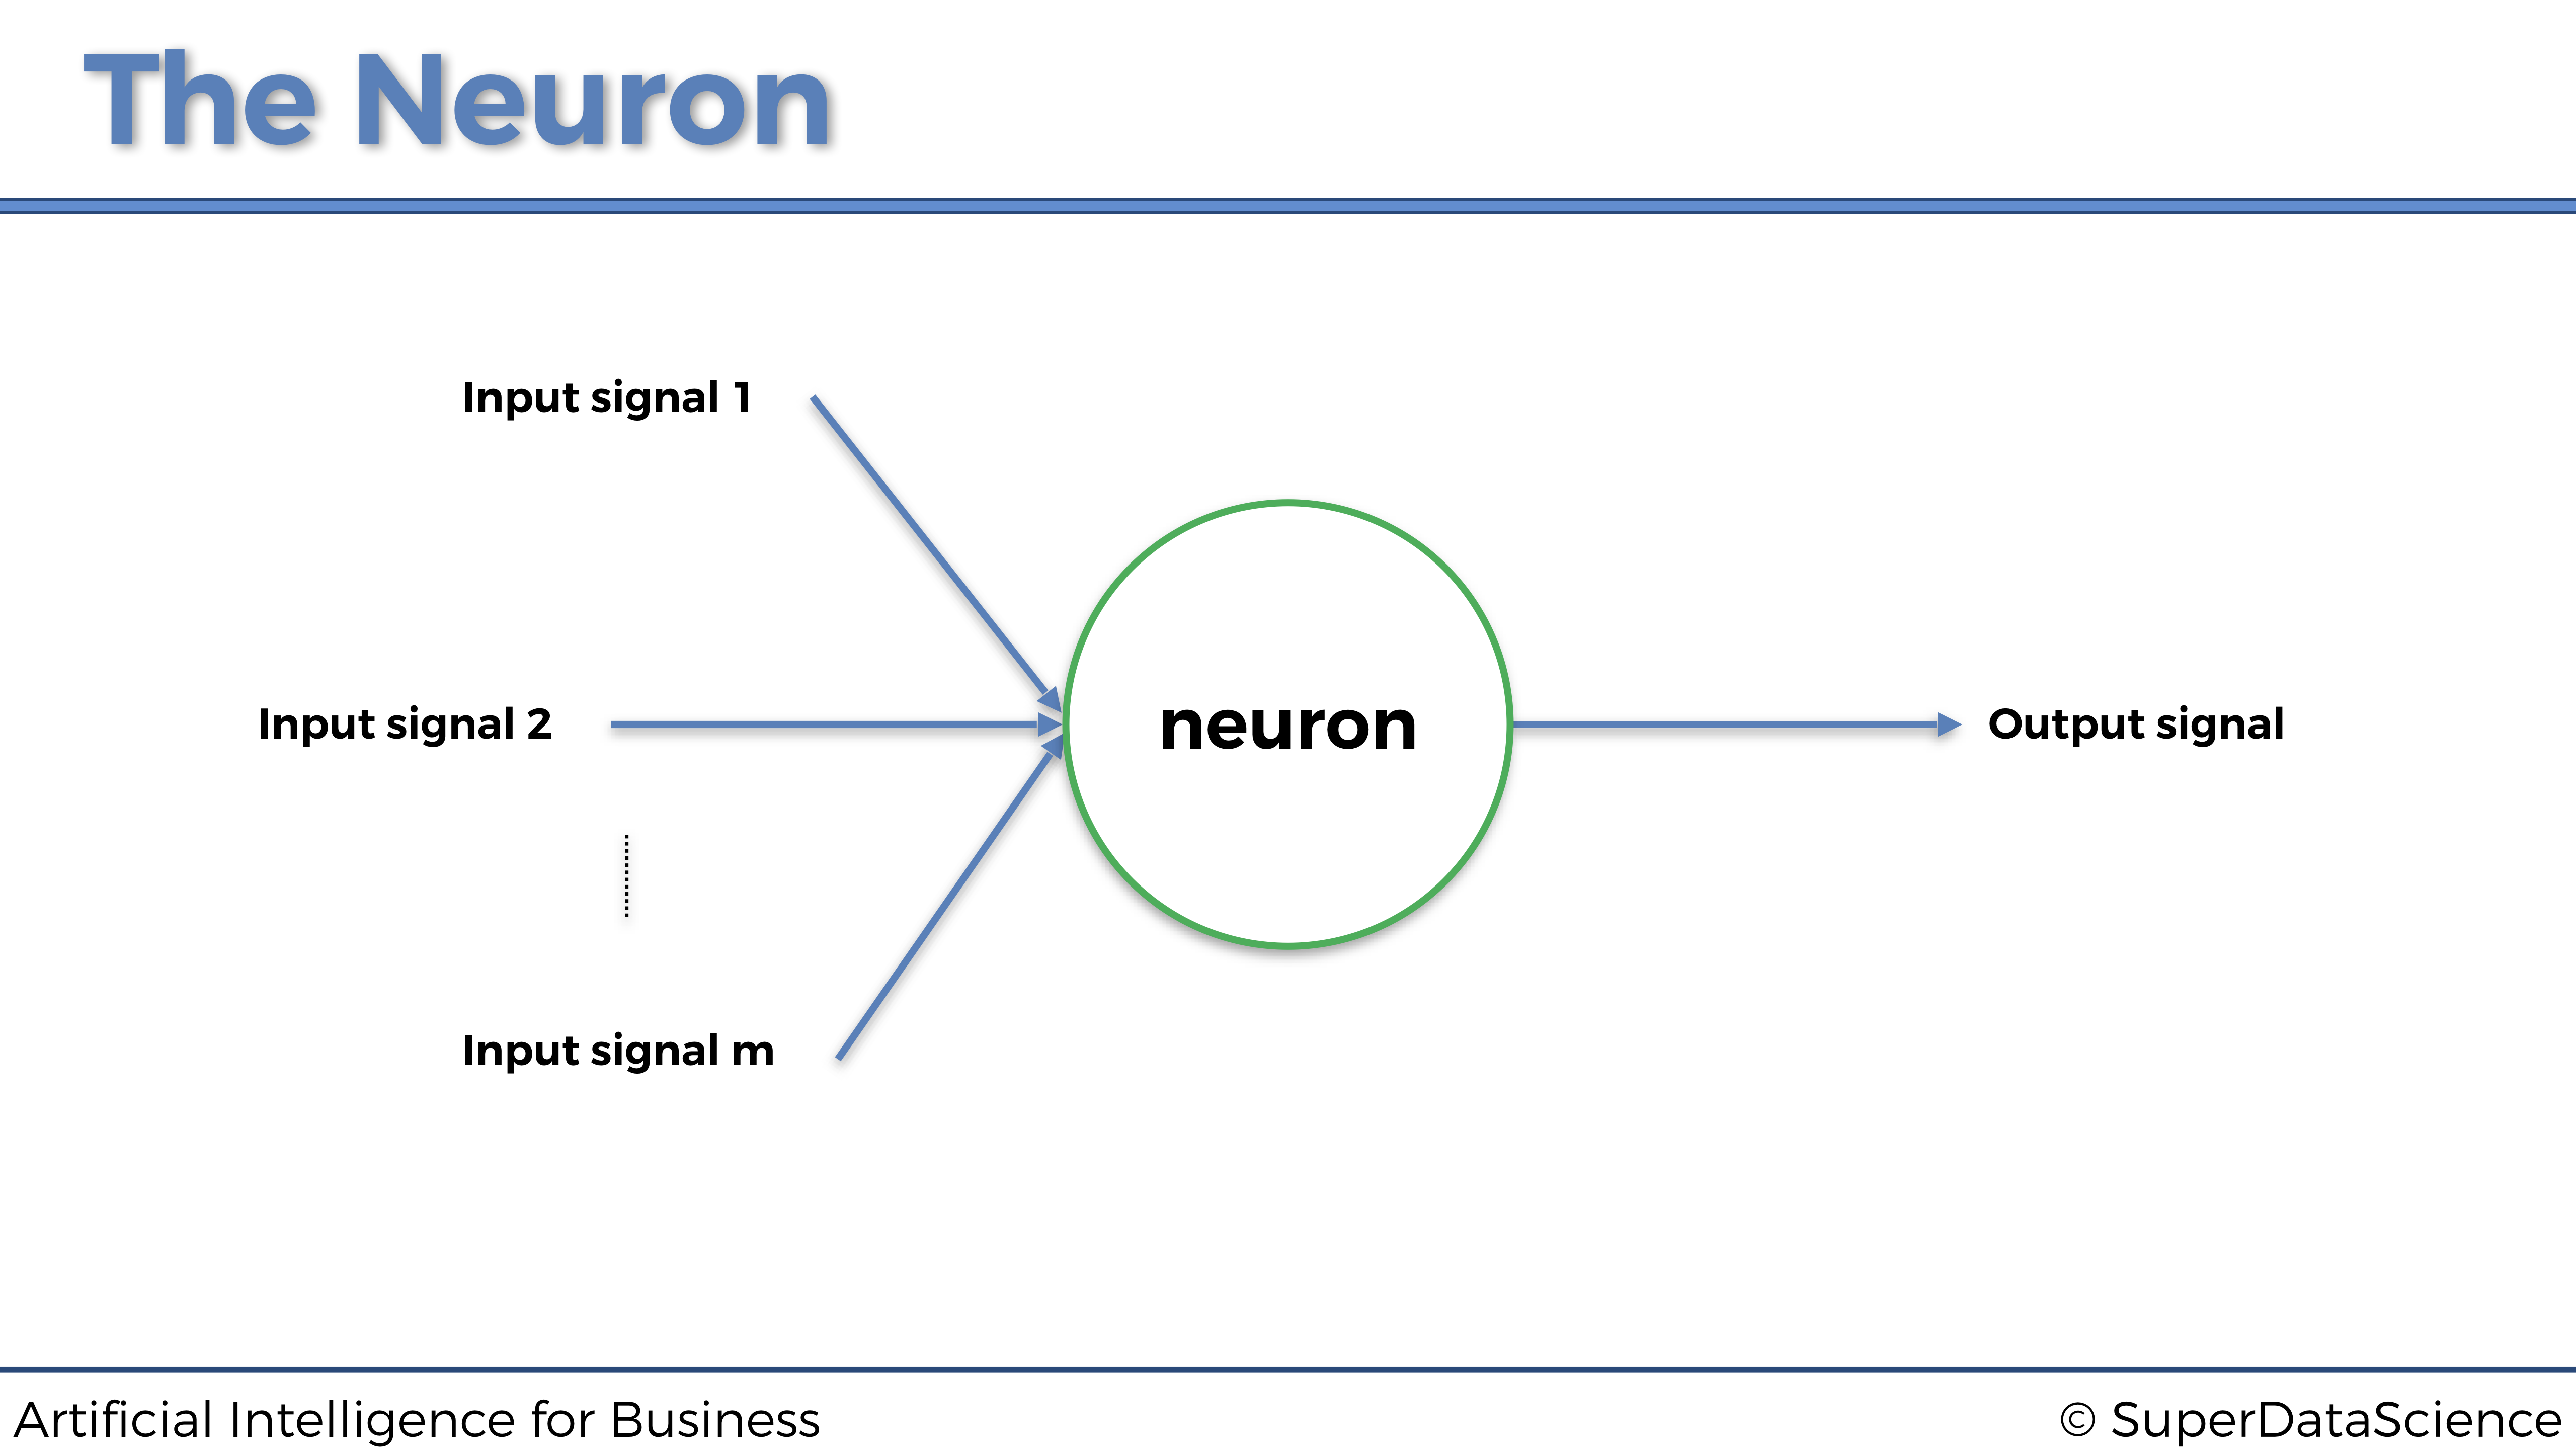
\includegraphics[scale=0.175]{ANN_5.png}
        \end{center}
\end{figure}

Just as a human neuron, it gets some input signals and it has an output signal. The blue arrow connecting the input signals to the neuron, and the neuron to the output signal, are like the synapses in the human neuron. But here in the machine neuron, what are exactly going to be these input and output signals? Well, the input signals are going to be the scaled independent variables composing the states of the environment, which remember in the case study are the temperature of the server, the number of users and the rate of data transmission, and the output signal will be the output values, which in the Deep Q-Learning model are always the Q-Values. Hence we get the general representation of a neuron for machines:

\begin{figure}[!htbp]
        \begin{center}
            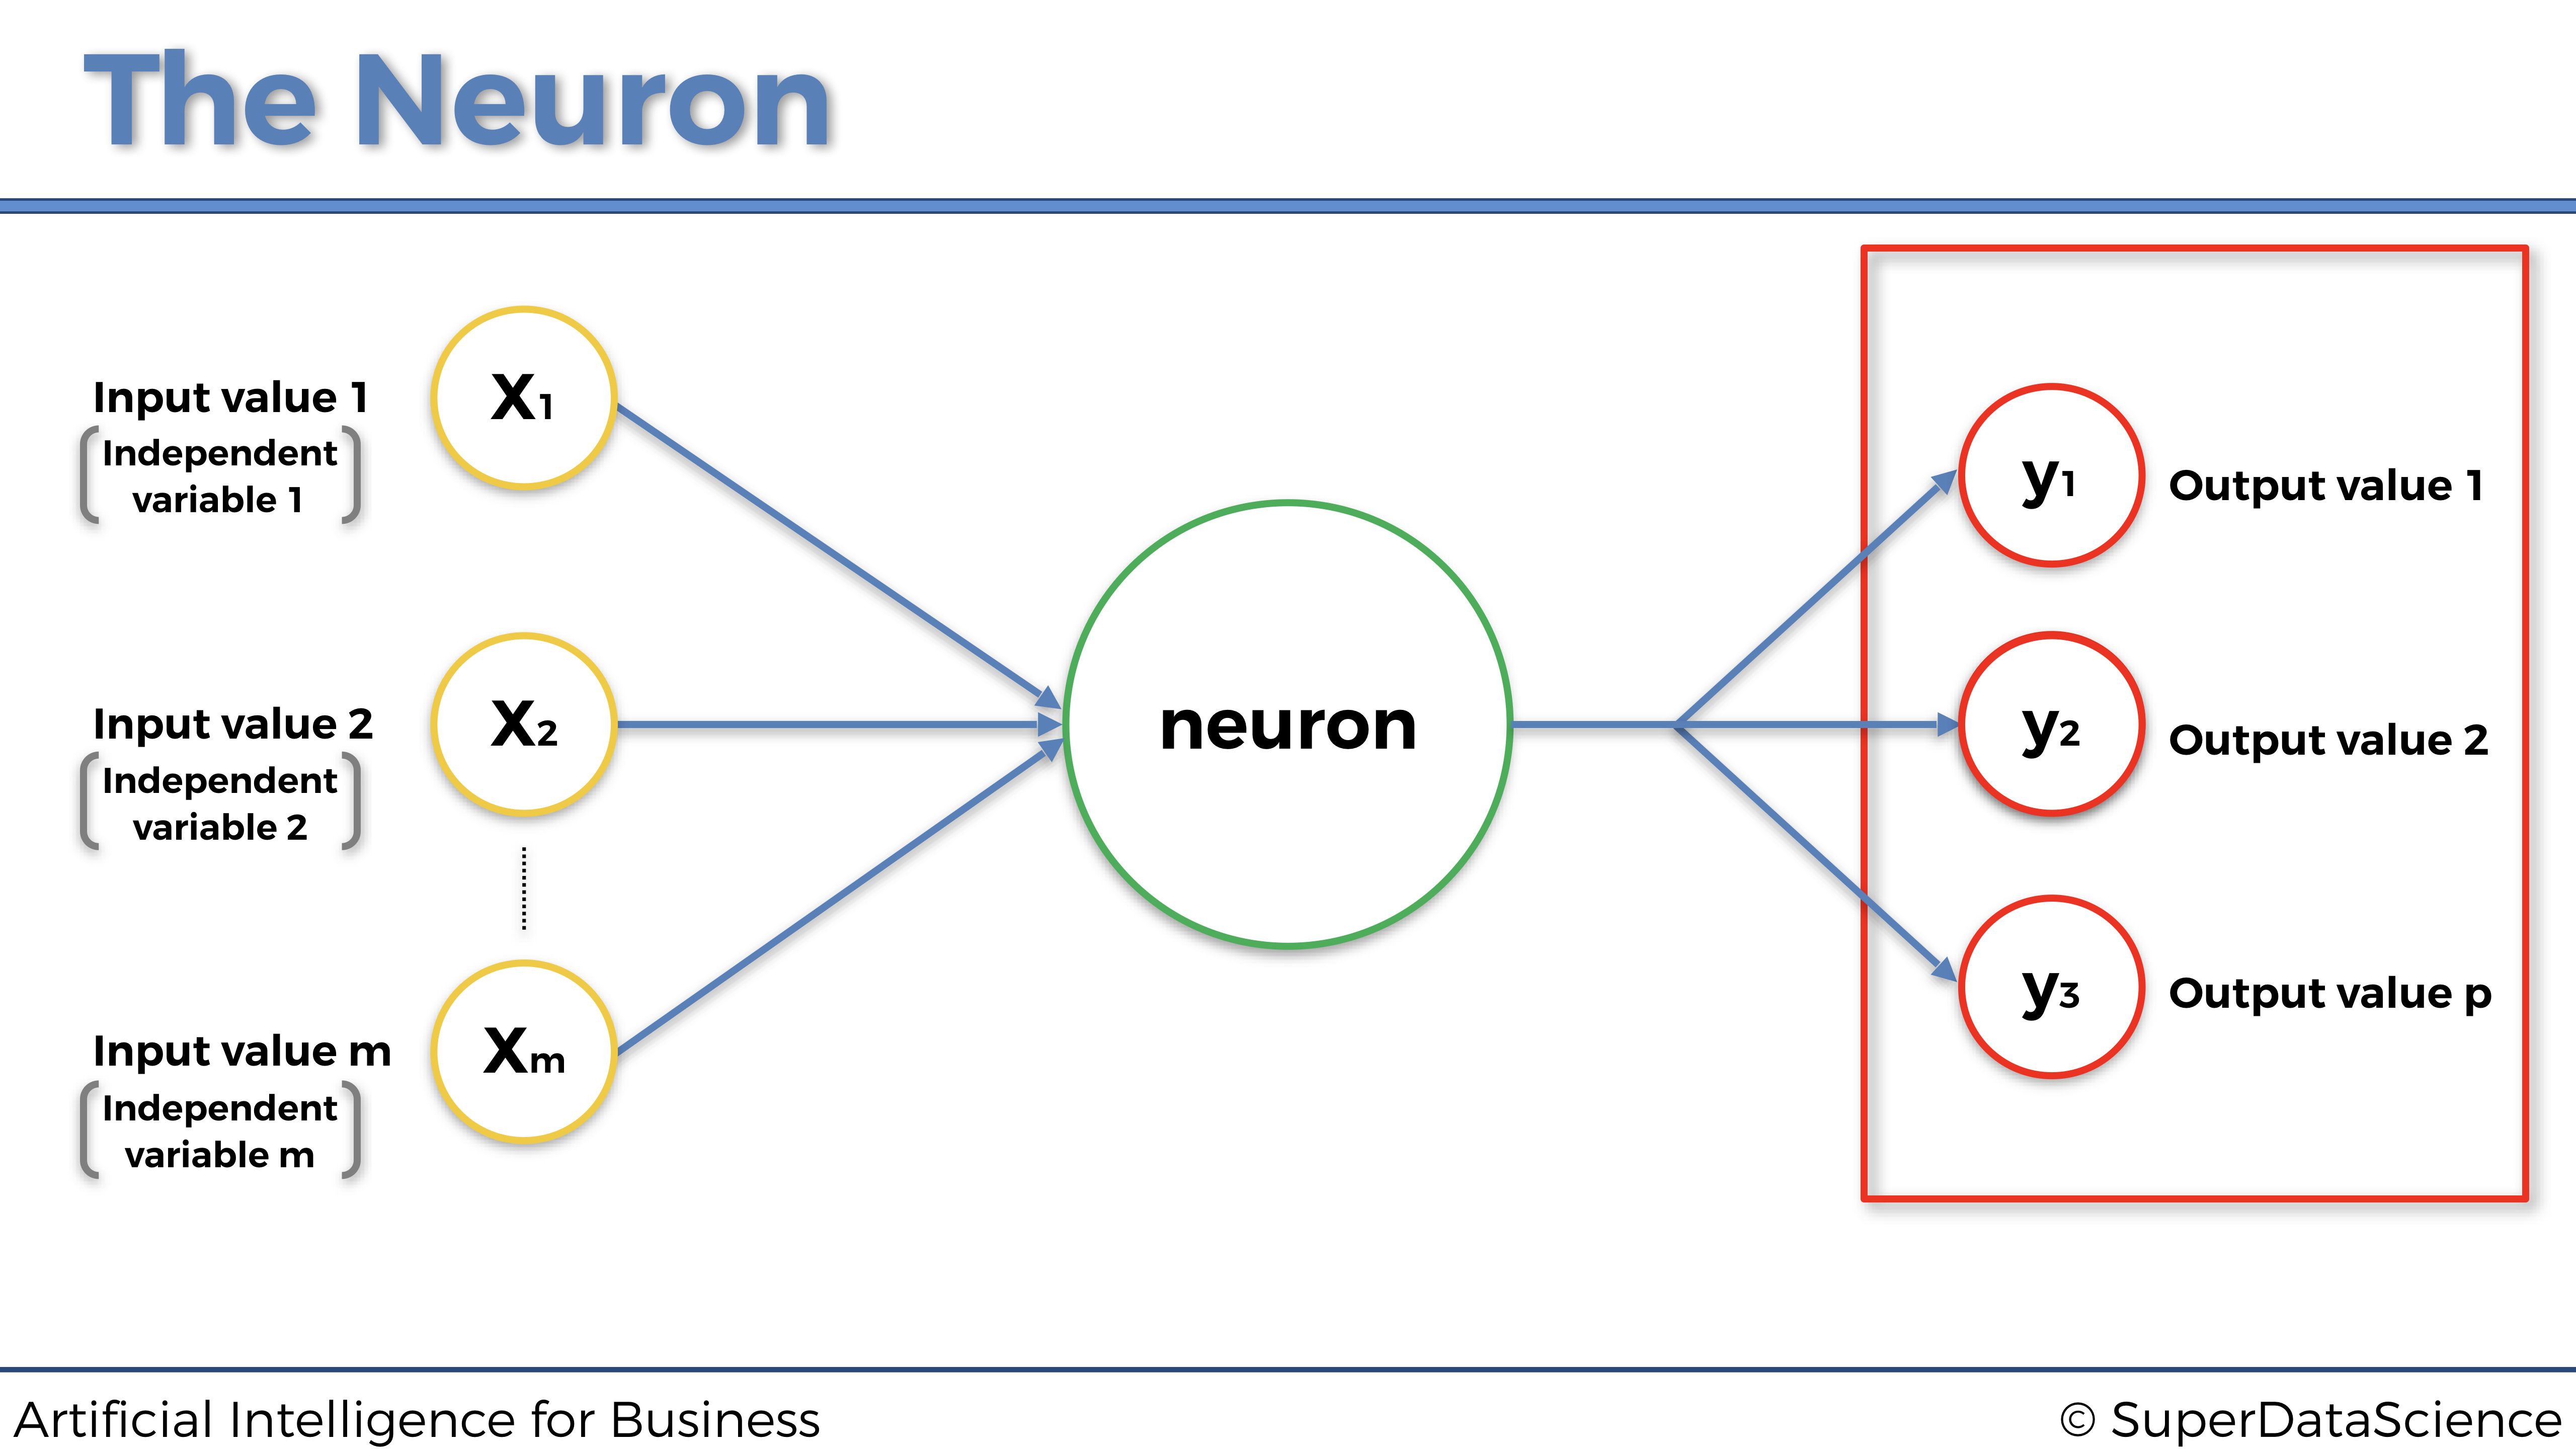
\includegraphics[scale=0.15]{ANN_7.png}
        \end{center}
\end{figure}

And now to finish with the neuron, let's add the last missing elements in this representation, but also the most important ones: the weights. Each synapse (blue arrow) will be attributed a weight. The larger is the weight, the stronger the signal will be through the synapse. And what is fundamental to understand is that, these weights, will be what the machine will update and update over time to improve the predictions. Let's represent them on the previous graphic, to make sure we all visualize them well:

\begin{figure}[!htbp]
        \begin{center}
            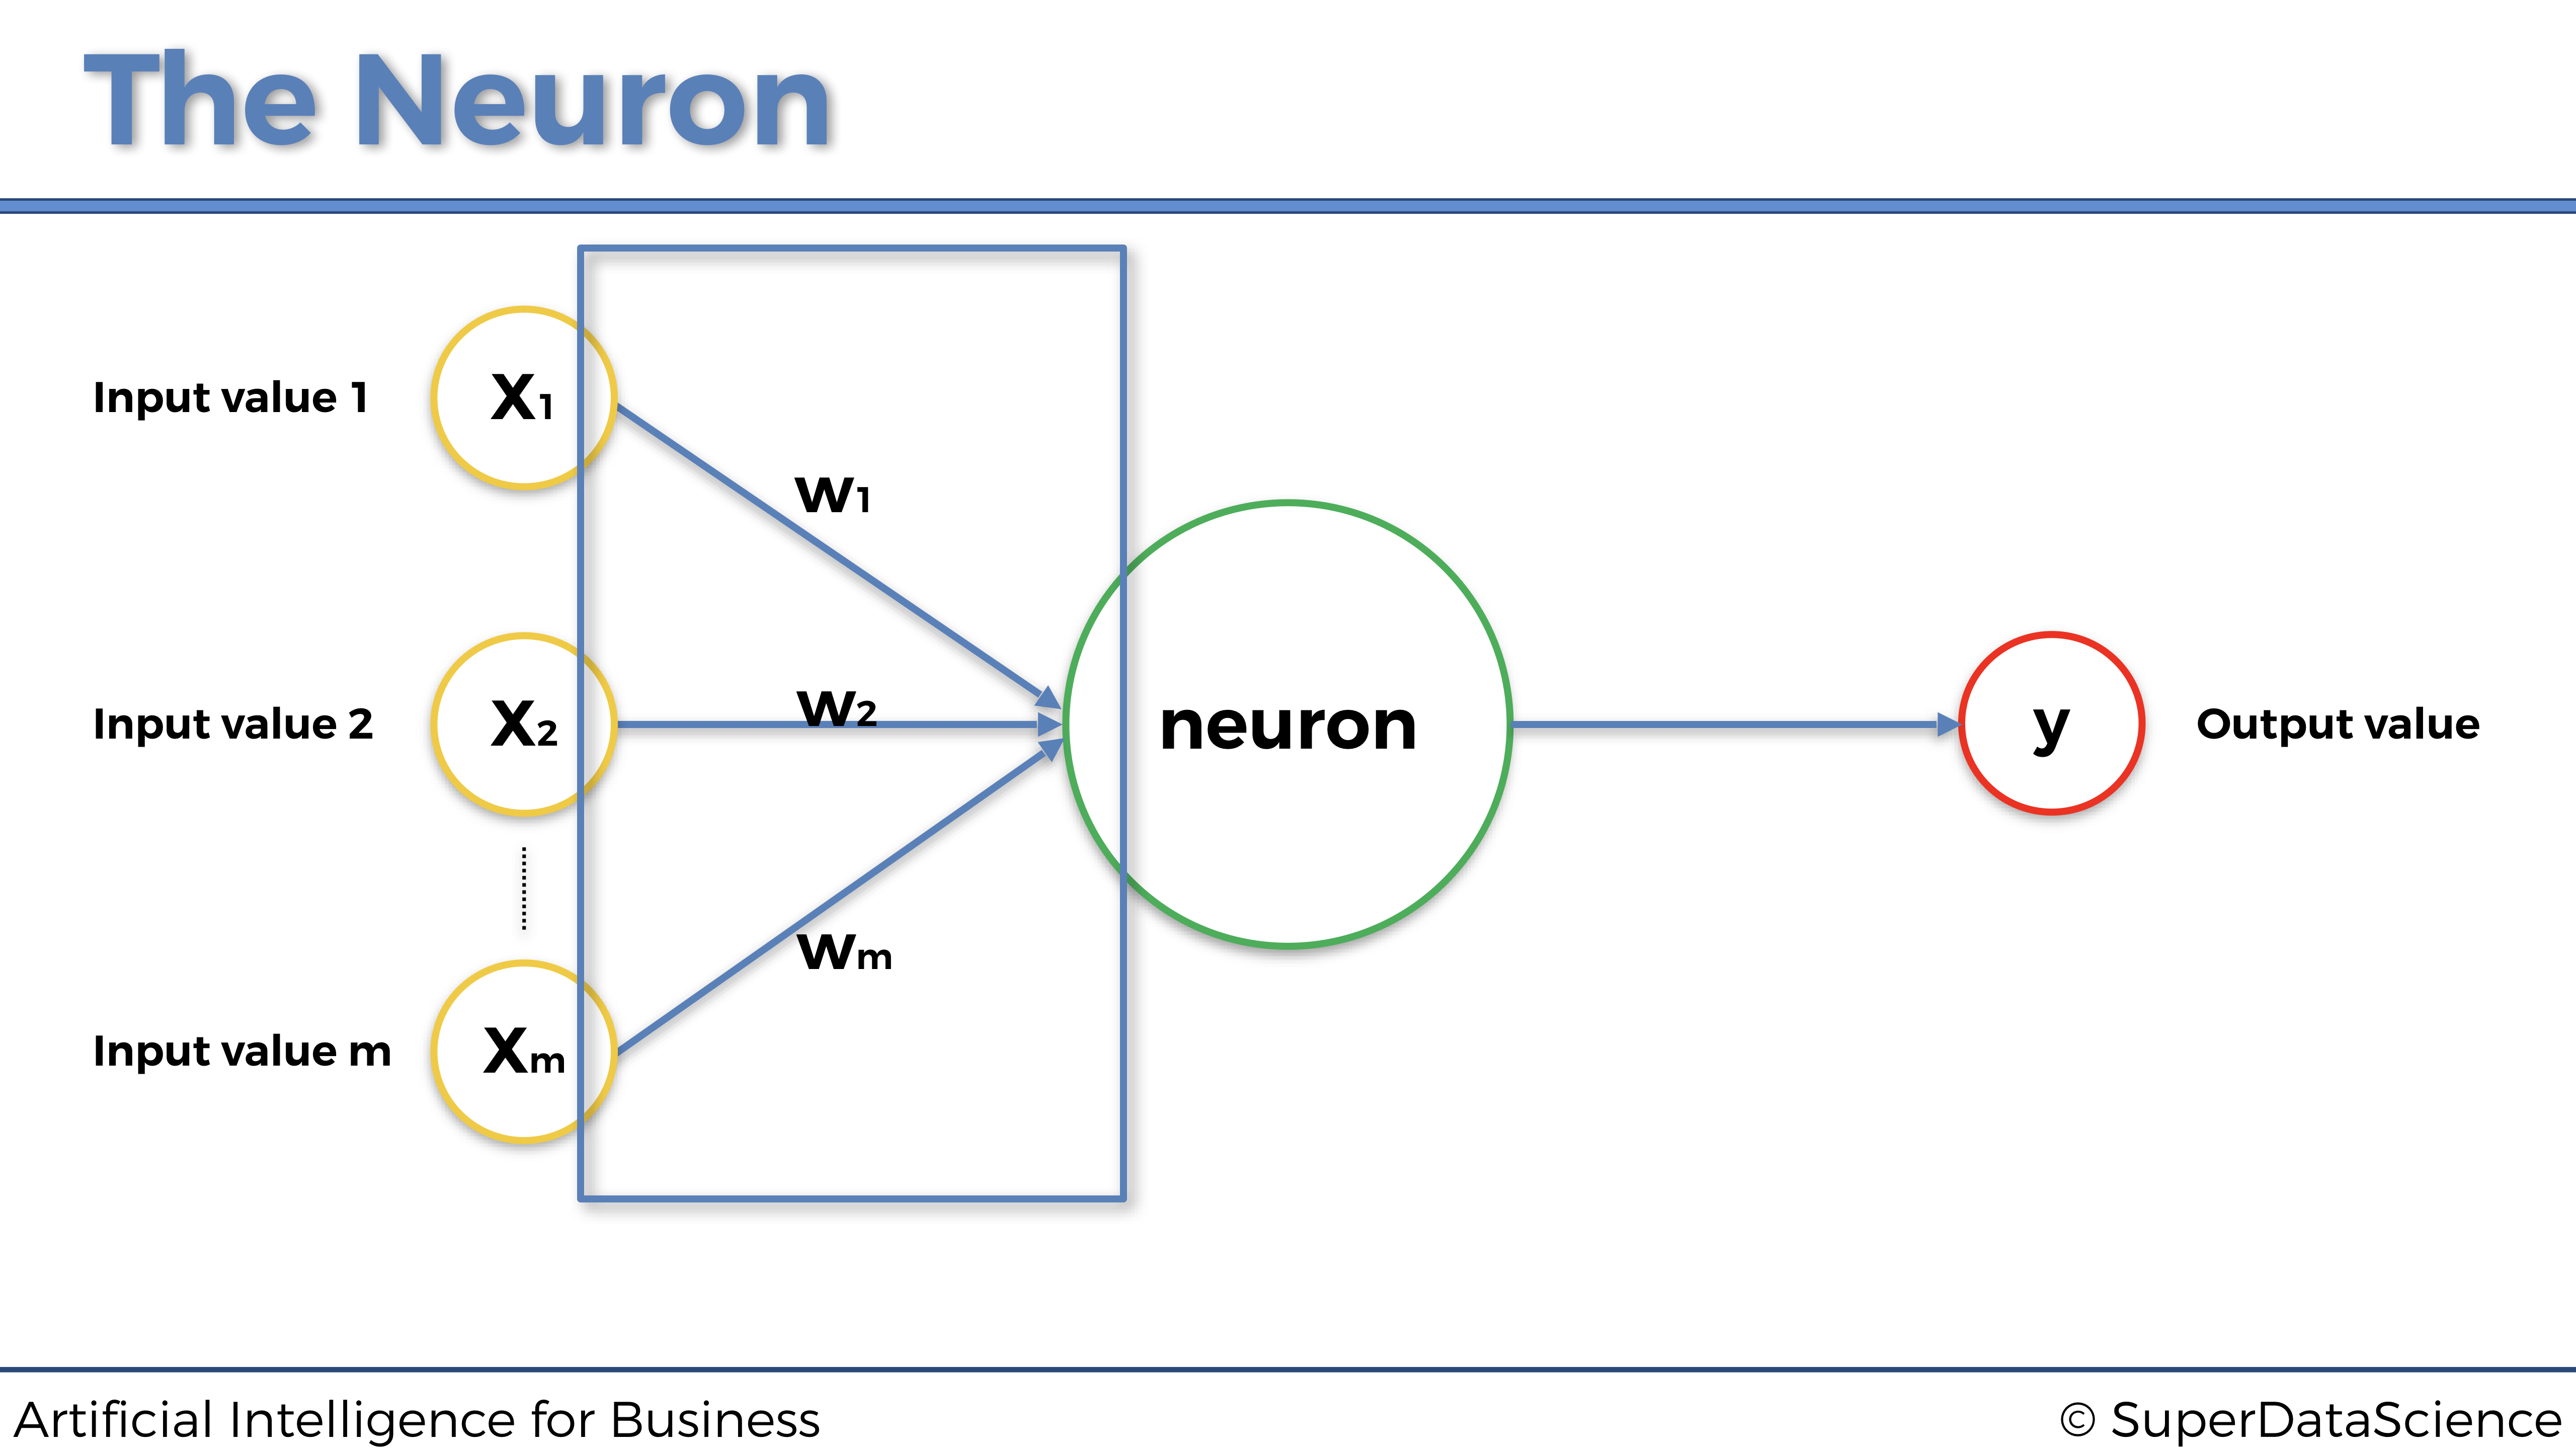
\includegraphics[scale=0.15]{ANN_8.png}
        \end{center}
\end{figure}

\subsection{The Activation Function}

The Activation Function is the function \(\phi\) operating inside the neuron, that will take as inputs the linear sum of the input values multiplied by their associated weights, and that will return the output value:

\begin{figure}[!htbp]
        \begin{center}
            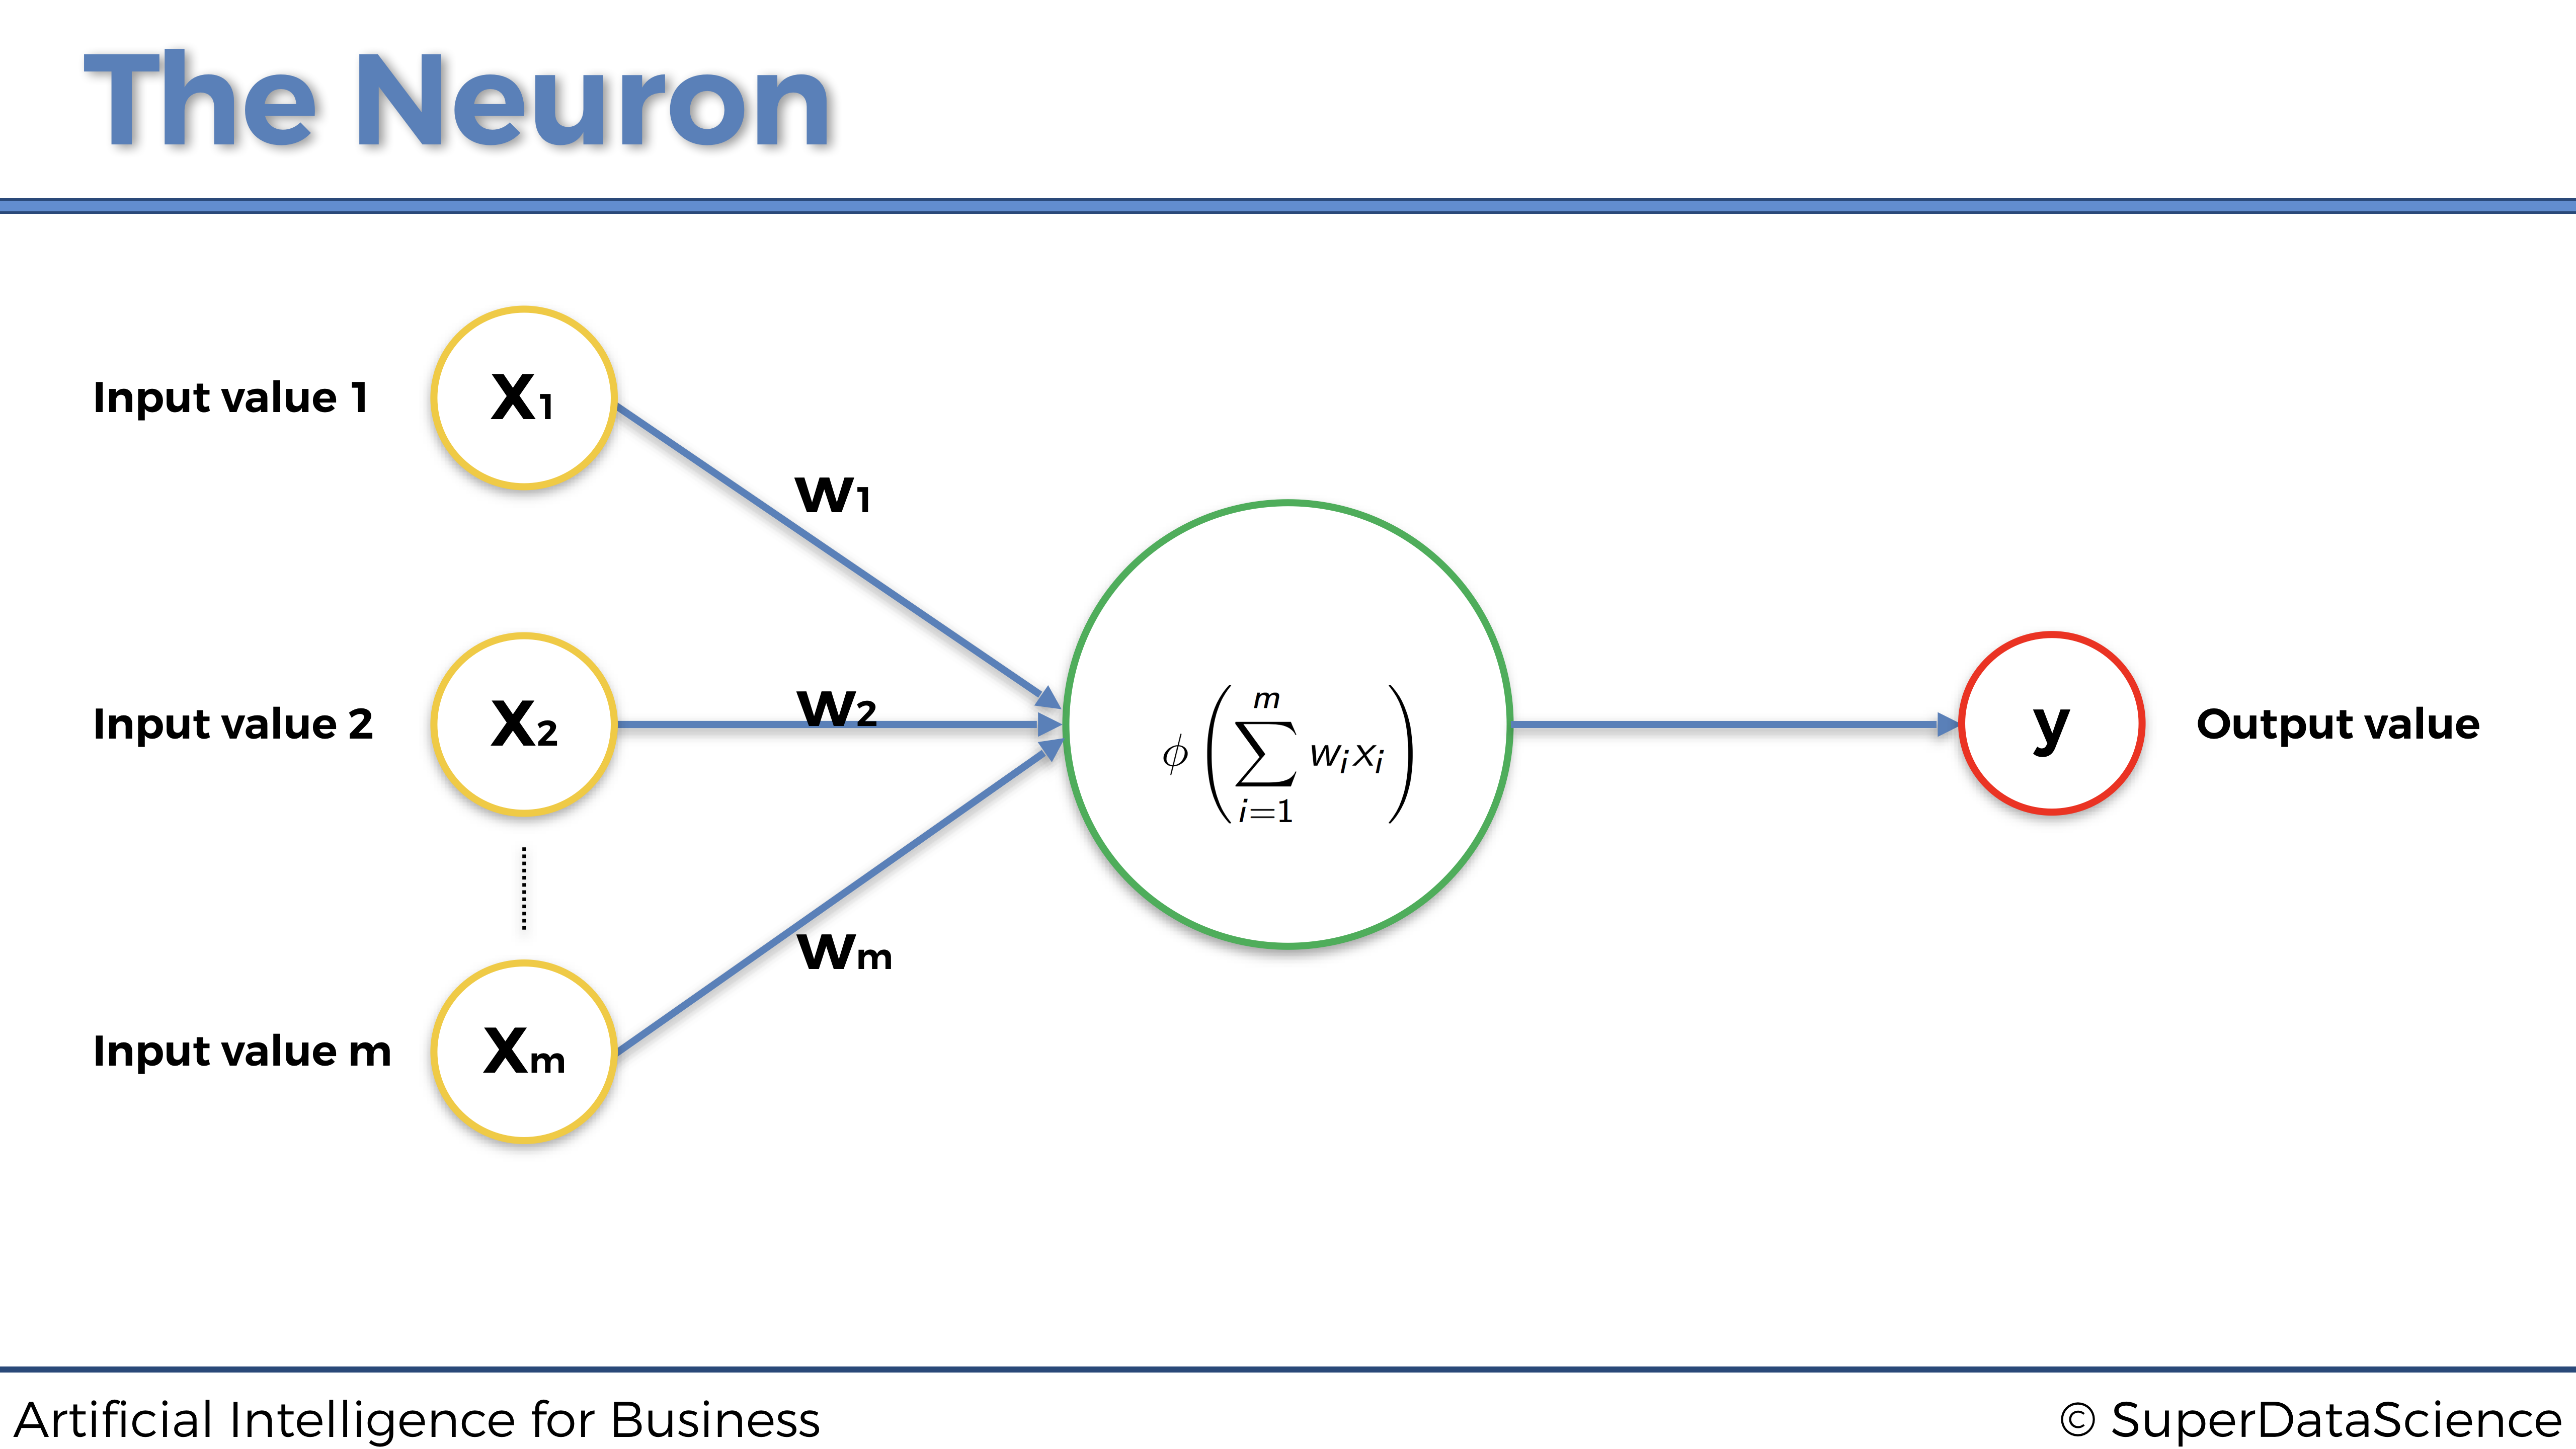
\includegraphics[scale=0.18]{ANN_9.png}
        \end{center}
\end{figure}

such that:

\begin{equation*}
    y = \phi\left( \sum_{i=1}^m w_i x_i \right)
\end{equation*}

Now what exactly is going to be the function \(\phi\)?

There can be many of them, but let's give the four most used ones, including of course the one we used in Part 2 - Minimizing Costs:

\begin{enumerate}
    \item The Threshold Activation Function
    \item The Sigmoid Activation Function
    \item The Rectifier Activation Function
    \item The Hyperbolic Tangent Activation Function
\end{enumerate}

Let's have a look at them one by one.

\newpage

\subsubsection{The Threshold Activation Function}

The Threshold Activation Function is simply defined by the following:

\begin{equation*}
    \phi(x) =
    \begin{cases}
        1 \textrm{ if } x \ge 0 \\
        0 \textrm{ if } x < 0
    \end{cases}
\end{equation*}

so that we get the following curve:

\begin{figure}[!htbp]
        \begin{center}
            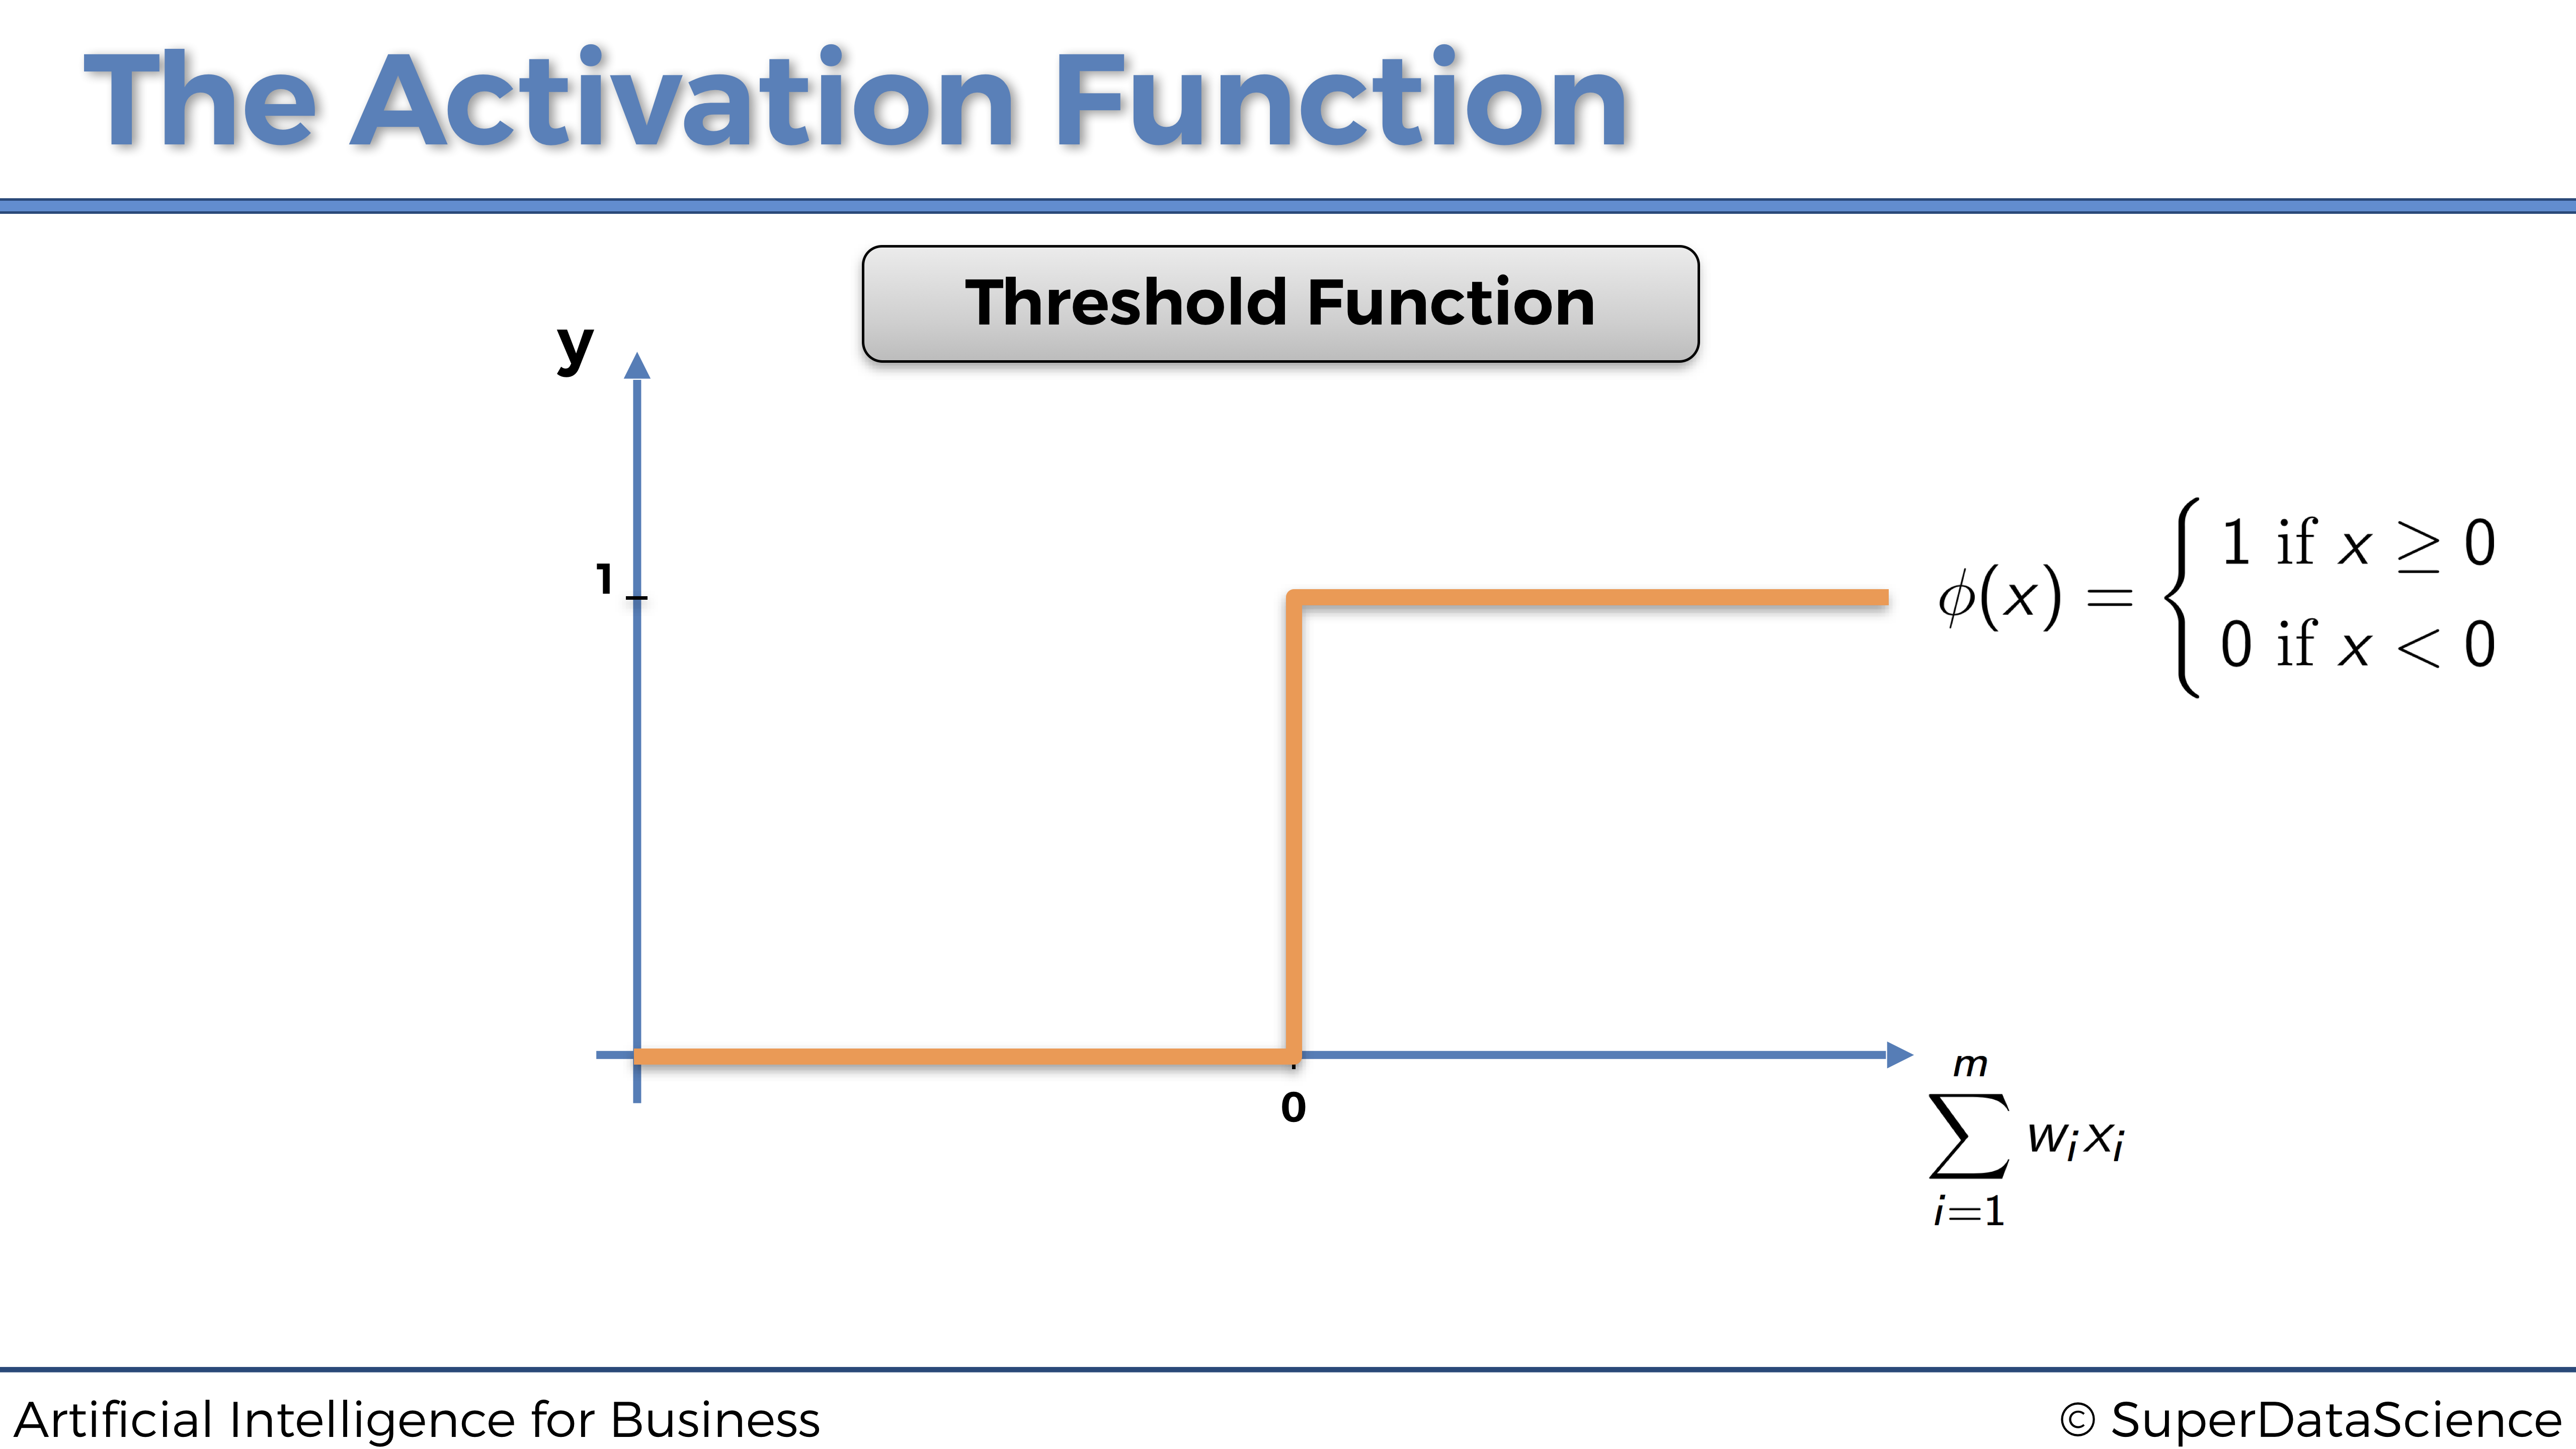
\includegraphics[scale=0.18]{ANN_10.png}
        \end{center}
\end{figure}

This means that the signal passing through the neuron will be discontinuous, and will only be activated if:

\begin{equation*}
    \sum_{i=1}^m w_i x_i \ge 0
\end{equation*}

Now let's have a look at the next activation function: the Sigmoid Activation function.

The Sigmoid Activation Function is the most effective and widely used one in Artificial Neural Networks, but mostly inside the last hidden layer (if we are dealing with a Deep Neural Network composed of several hidden layers) passing the signal towards the output layer.

\newpage

\subsubsection{The Sigmoid Activation Function}

The Sigmoid Activation Function is defined by the following:

\begin{equation*}
\phi(x) = \frac{1}{1+e^{-x}}
\end{equation*}

so that we get the following curve:

\begin{figure}[!htbp]
        \begin{center}
            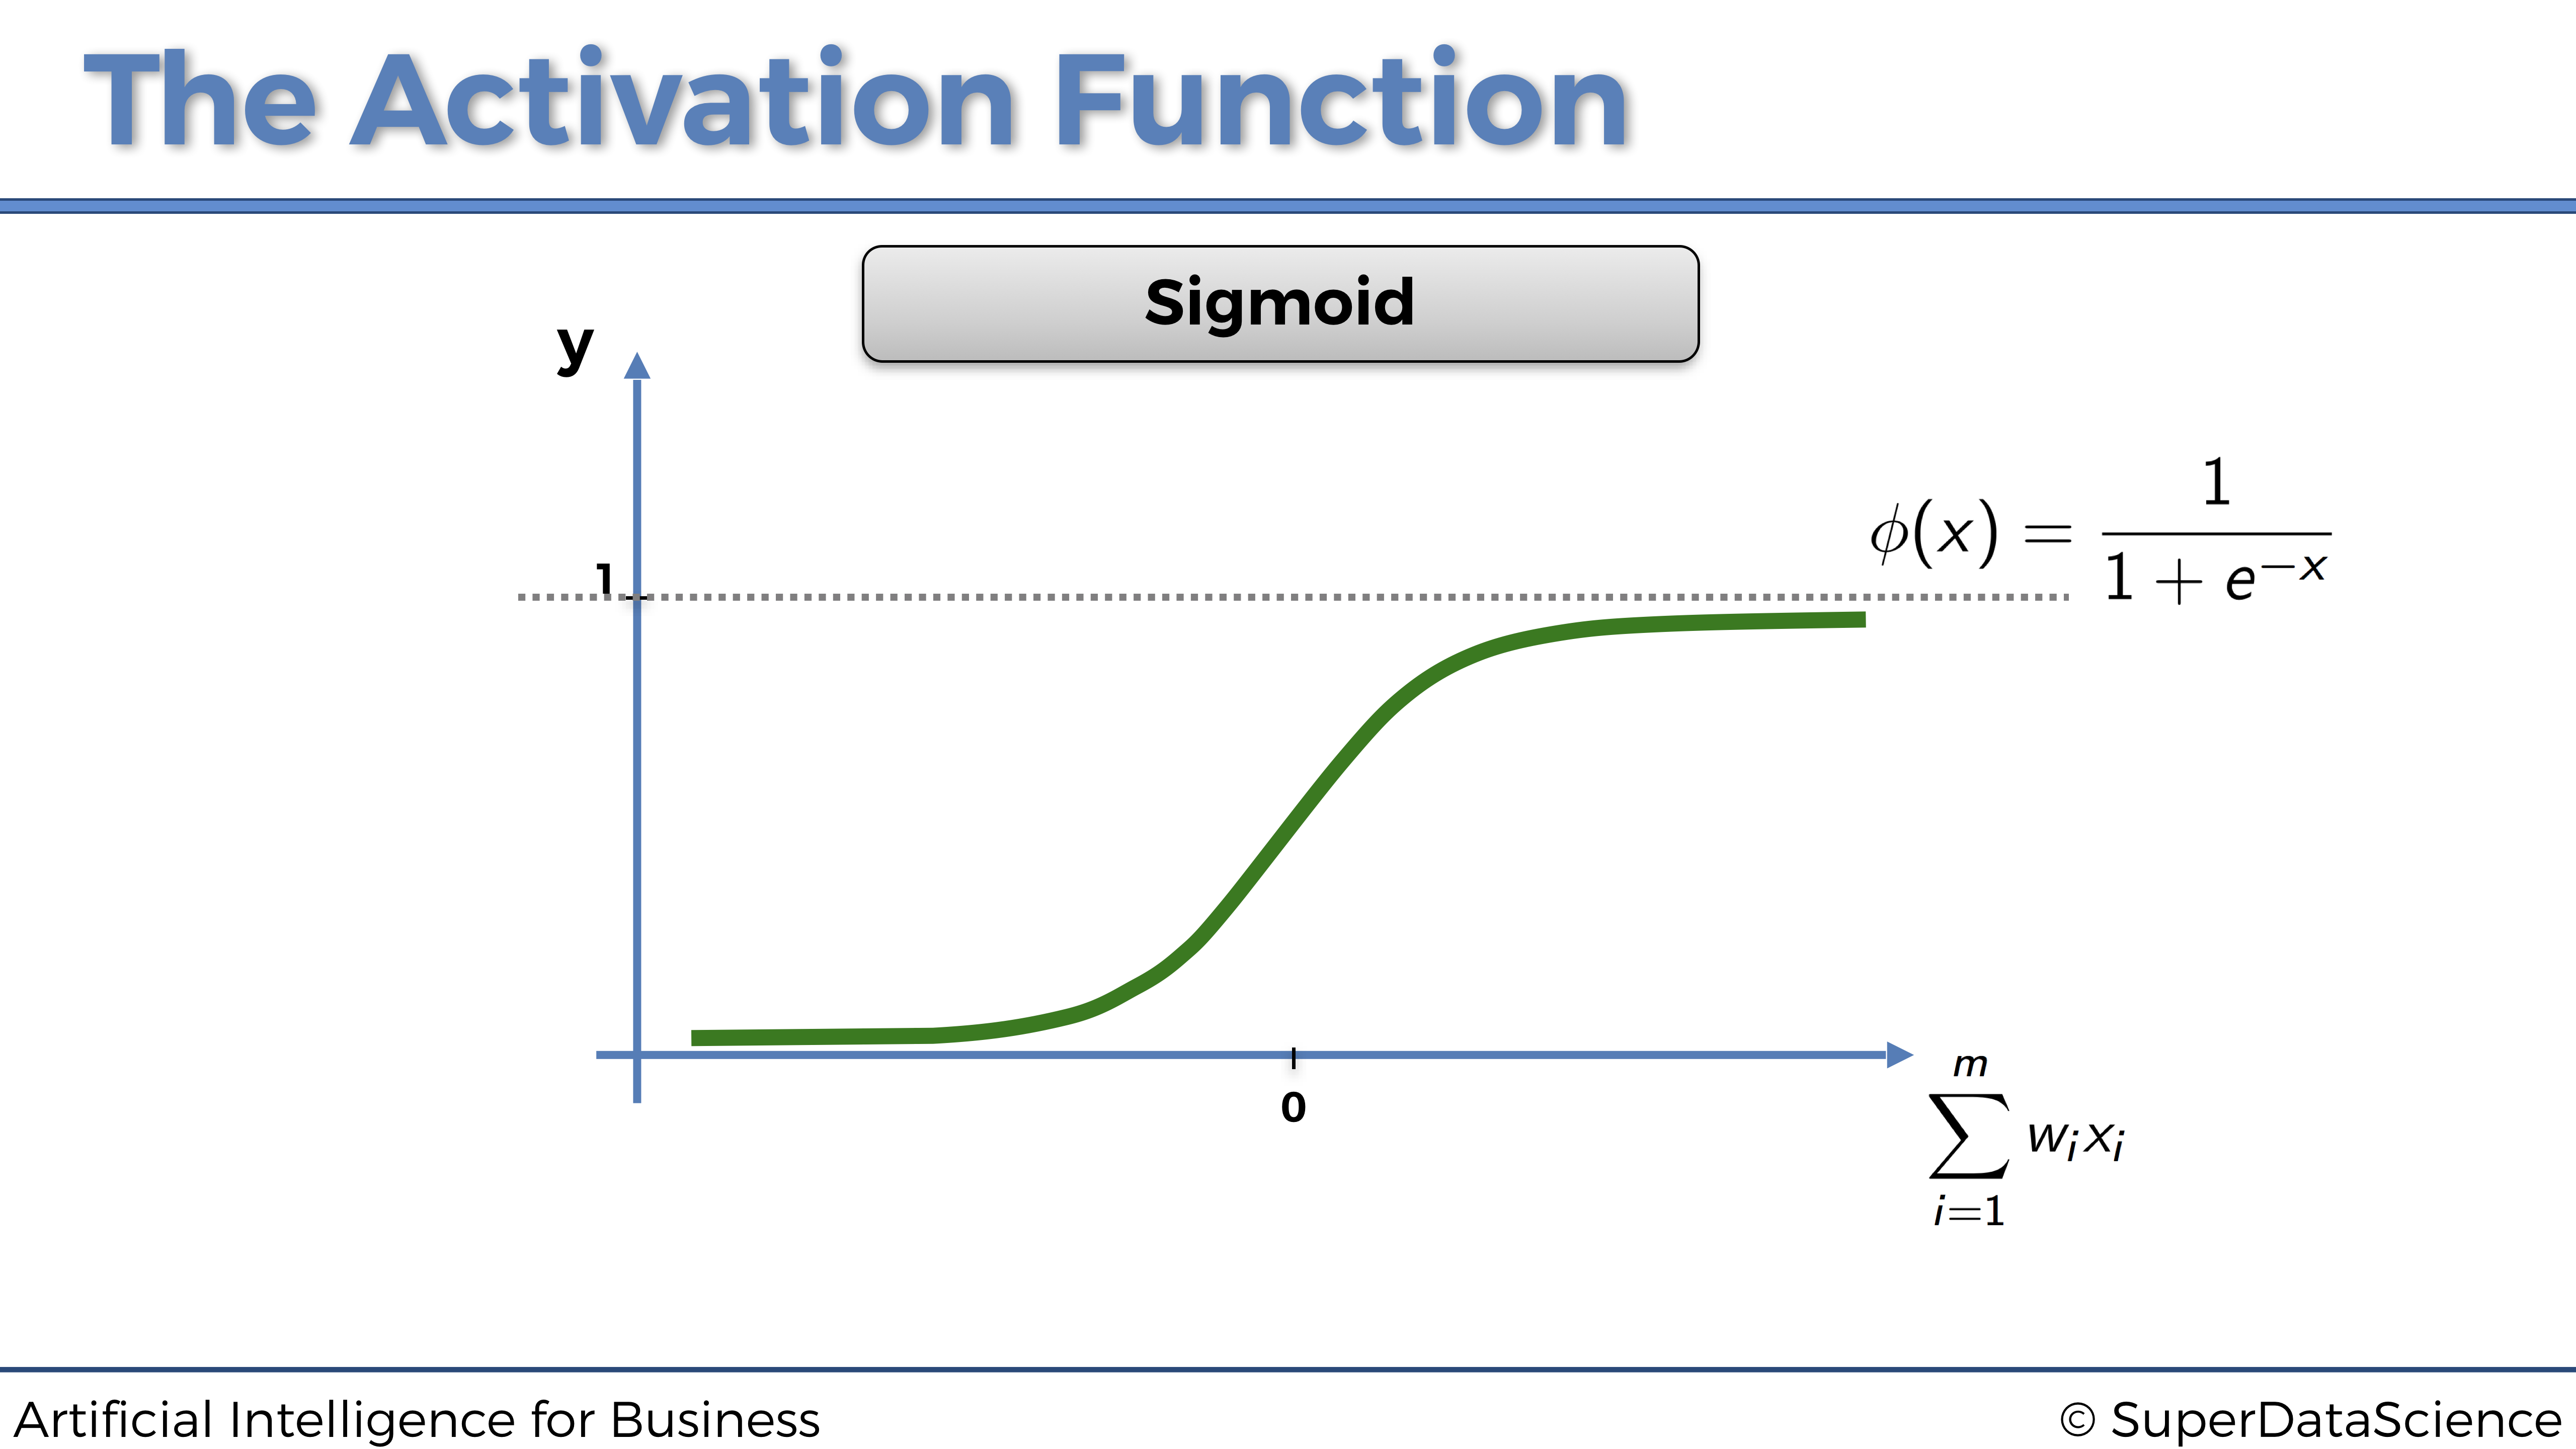
\includegraphics[scale=0.18]{ANN_11.png}
        \end{center}
\end{figure}

This means that the signal passing through the neuron will be continuous and will always be activated. And the higher is \(\sum_{i=1}^m w_i x_i\), the stronger will be that signal.

Now let's have a look at another widely used activation function: the Rectifier Activation function.

You will find it in most of the \underline{DEEP} Neural Networks, but mostly inside the hidden layers, as opposed to the sigmoid function which is rather used for the output layer.

\newpage

\subsubsection{The Rectifier Activation Function}

The Threshold Activation Function is simply defined by the following:

\begin{equation*}
    \phi(x) = \max(x,0)
\end{equation*}

so that we get the following curve:

\begin{figure}[!htbp]
        \begin{center}
            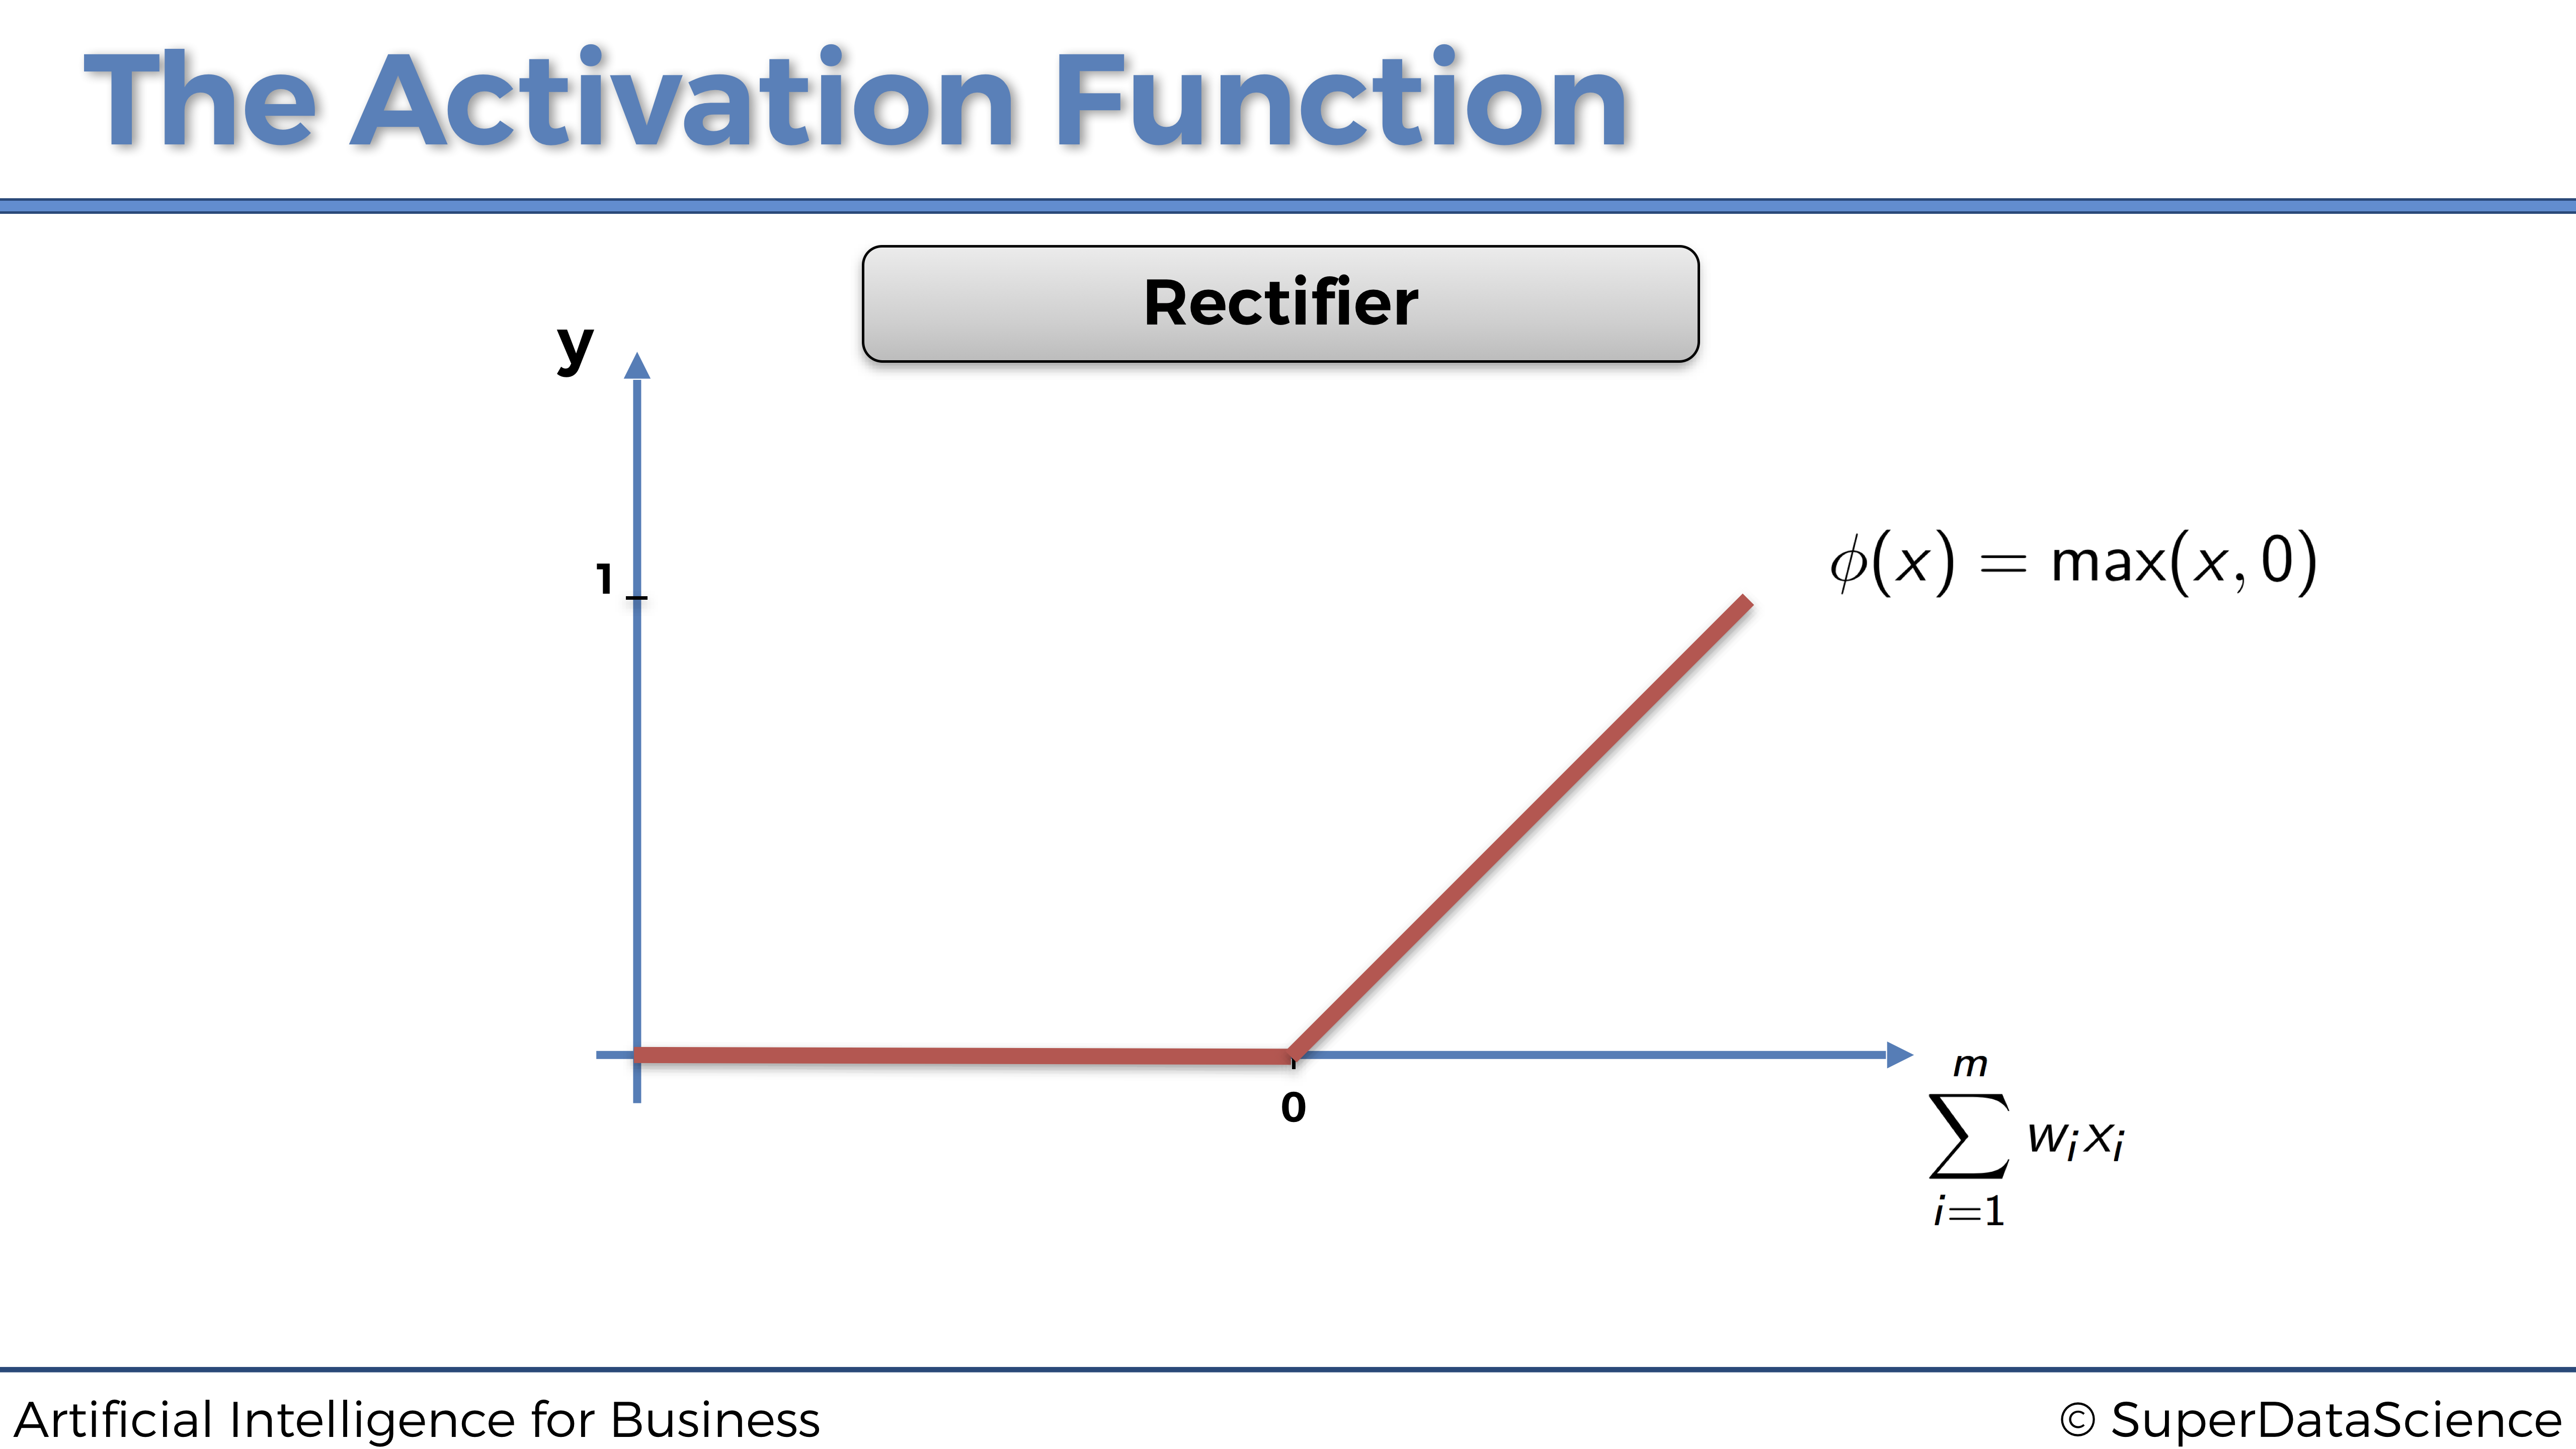
\includegraphics[scale=0.18]{ANN_12.png}
        \end{center}
\end{figure}

This means that the signal passing through the neuron will be continuous, and will only be activated if:

\begin{equation*}
    \sum_{i=1}^m w_i x_i \ge 0
\end{equation*}

And the higher is \(\sum_{i=1}^m w_i x_i\) above 0, the stronger will be that signal.

Now let's have a look at the next activation function: the Hyperbolic Tangent Activation function.

The Hyperbolic Tangent activation function is less widely used, though it can sometimes be a more relevant choice in some Artificial Neural Networks, especially when the inputs are standardized.

\newpage

\subsubsection{The Hyperbolic Tangent Activation Function}

The Hyperbolic Tangent Activation Function is defined by the following:

\begin{equation*}
    \phi(x) = \frac{1-e^{-2x}}{1+e^{-2x}}
\end{equation*}

so that we get the following curve:

\begin{figure}[!htbp]
        \begin{center}
            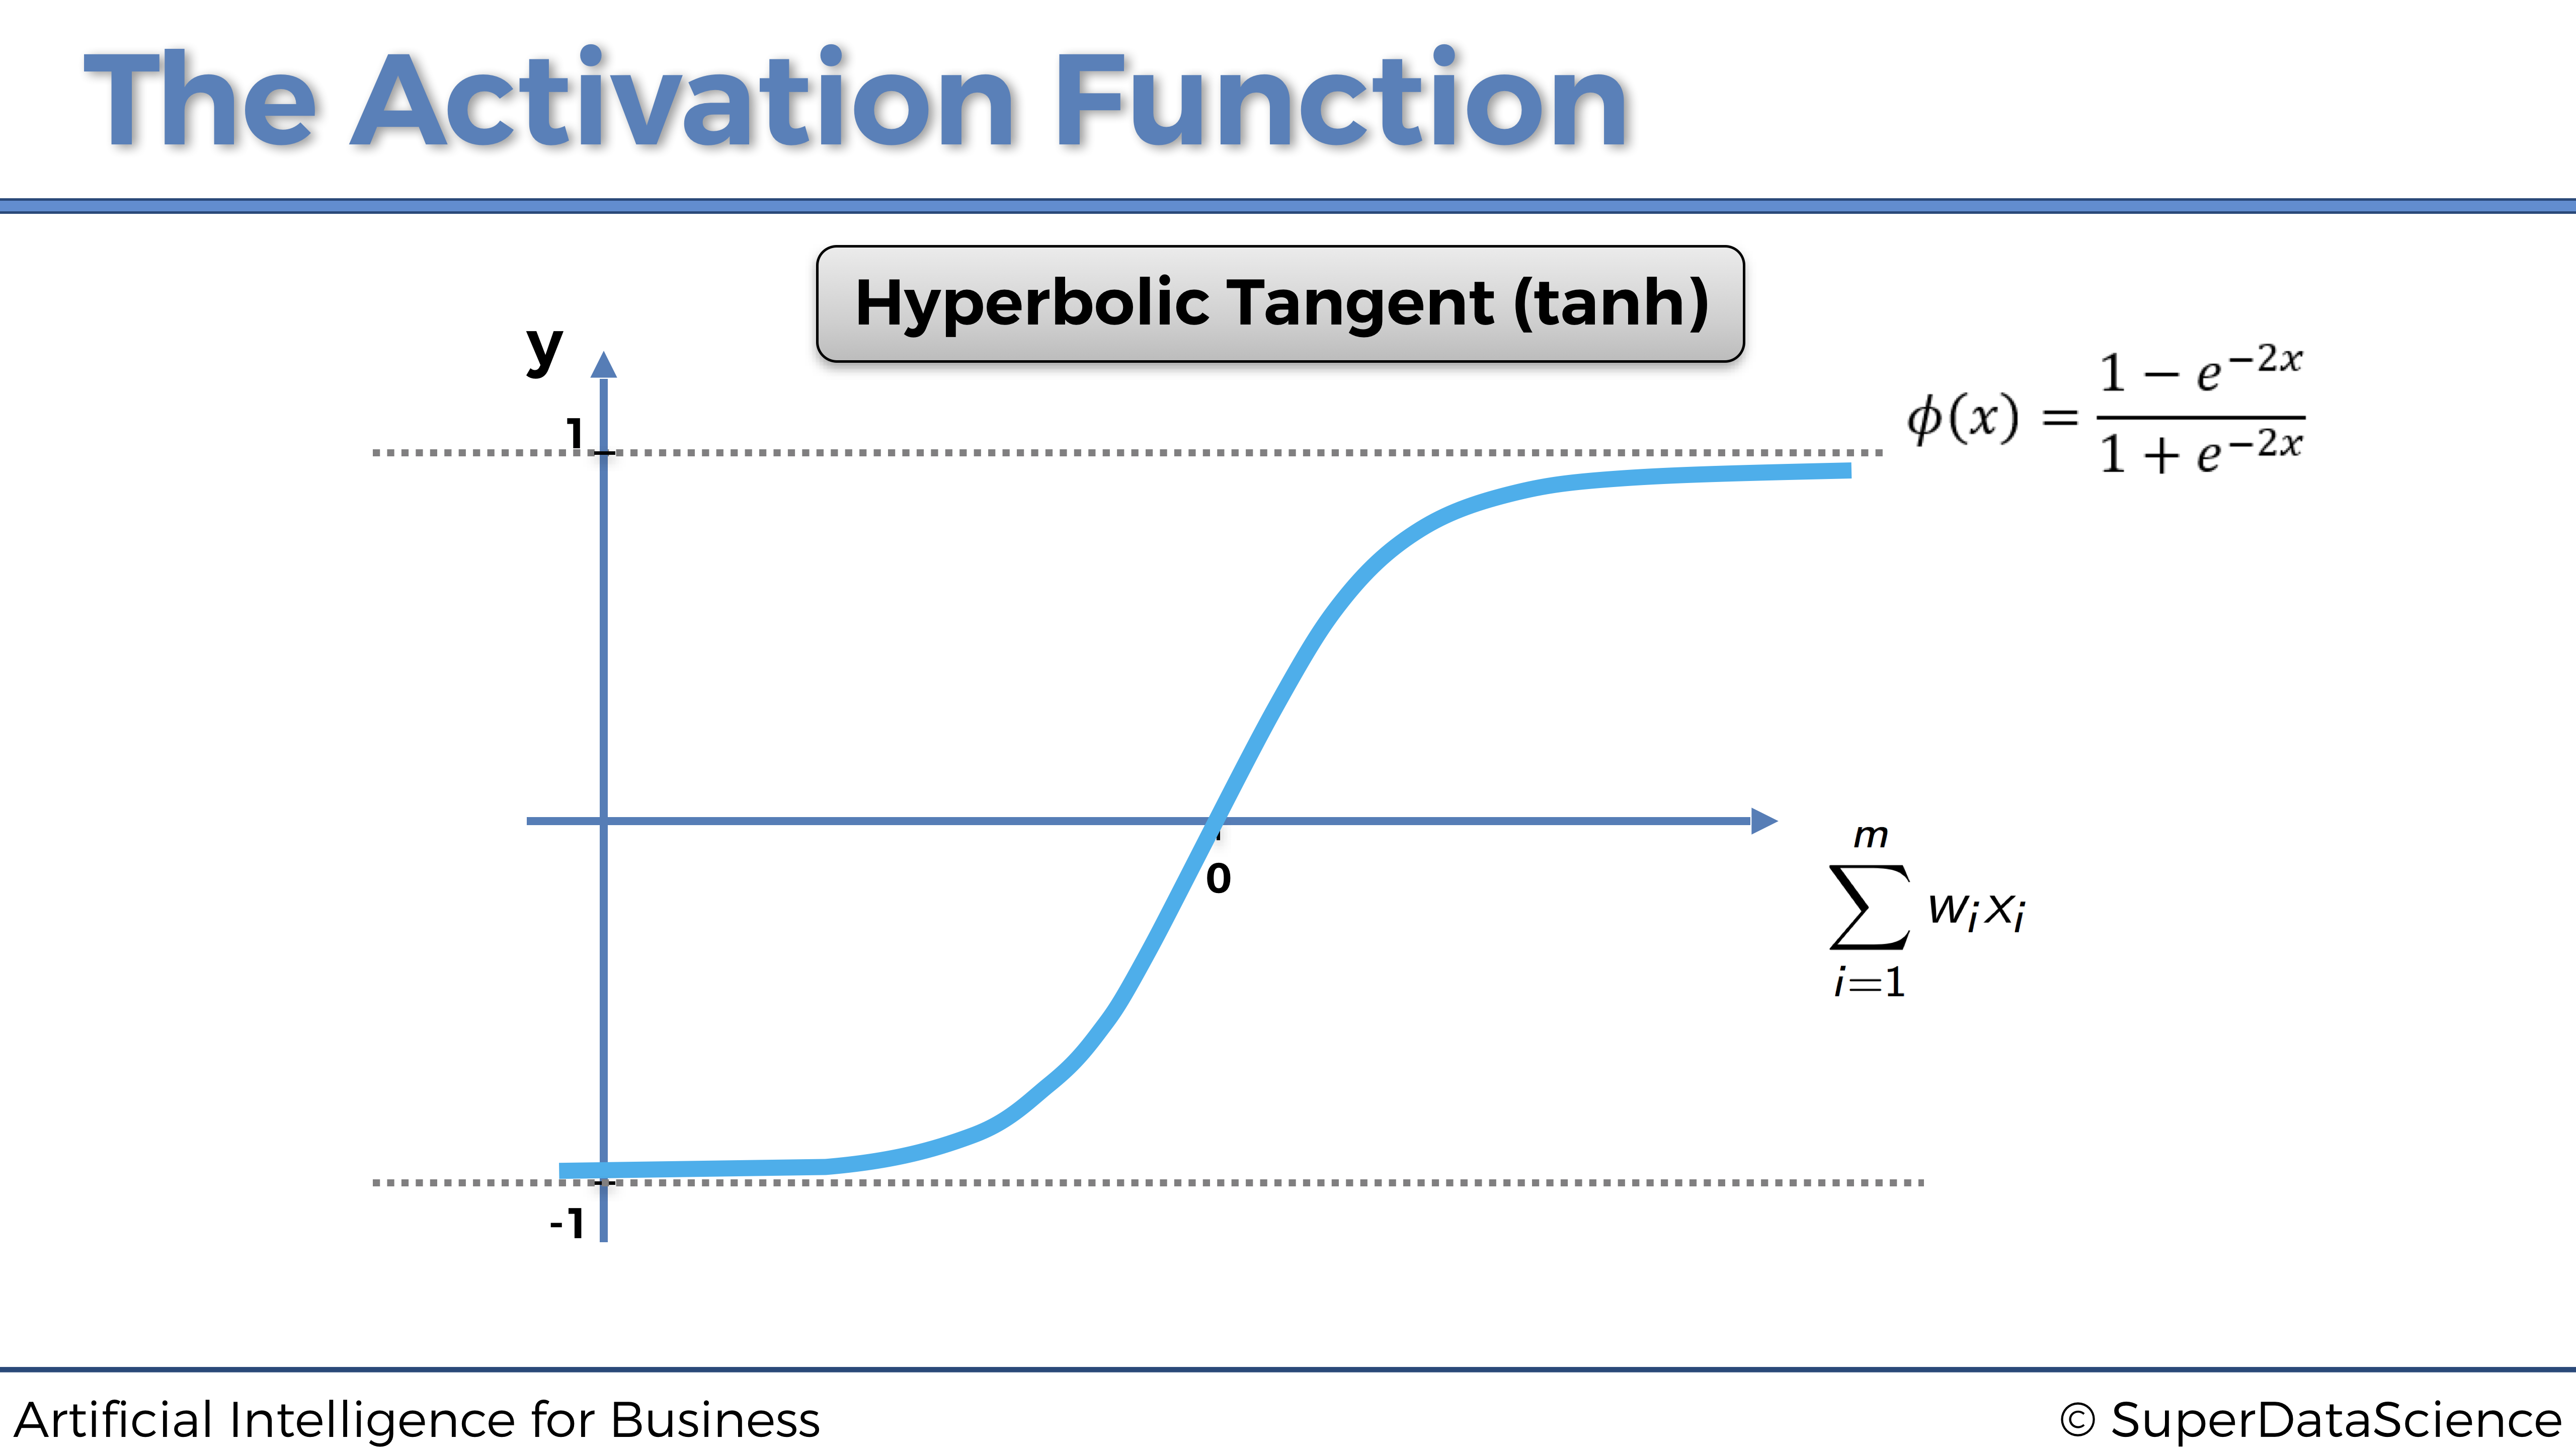
\includegraphics[scale=0.18]{ANN_13.png}
        \end{center}
\end{figure}

This means that the signal passing through the neuron will be continuous and will always be activated. The higher \(\sum_{i=1}^m w_i x_i\) is above 0, the stronger will be that signal. The lower \(\sum_{i=1}^m w_i x_i\) is below 0, the weaker will be that signal.

\newpage

So that raises the question: which activation function should we choose, or, more frequently asked, how do we know which one to choose?

Good news, the answer is simple, and let's give it inside a small blueprint.

That actually depends on what is returned as the dependent variable. If it is a binary outcome 0 or 1, then a good choice would be the threshold activation function. If what you want to be returned is the probability that the dependent variable is 1, then an excellent choice is the sigmoid activation function, since its sigmoid curve is a perfect fit to model probabilities.

Here is this small blueprint highlighted in this slide:

\begin{figure}[!htbp]
        \begin{center}
            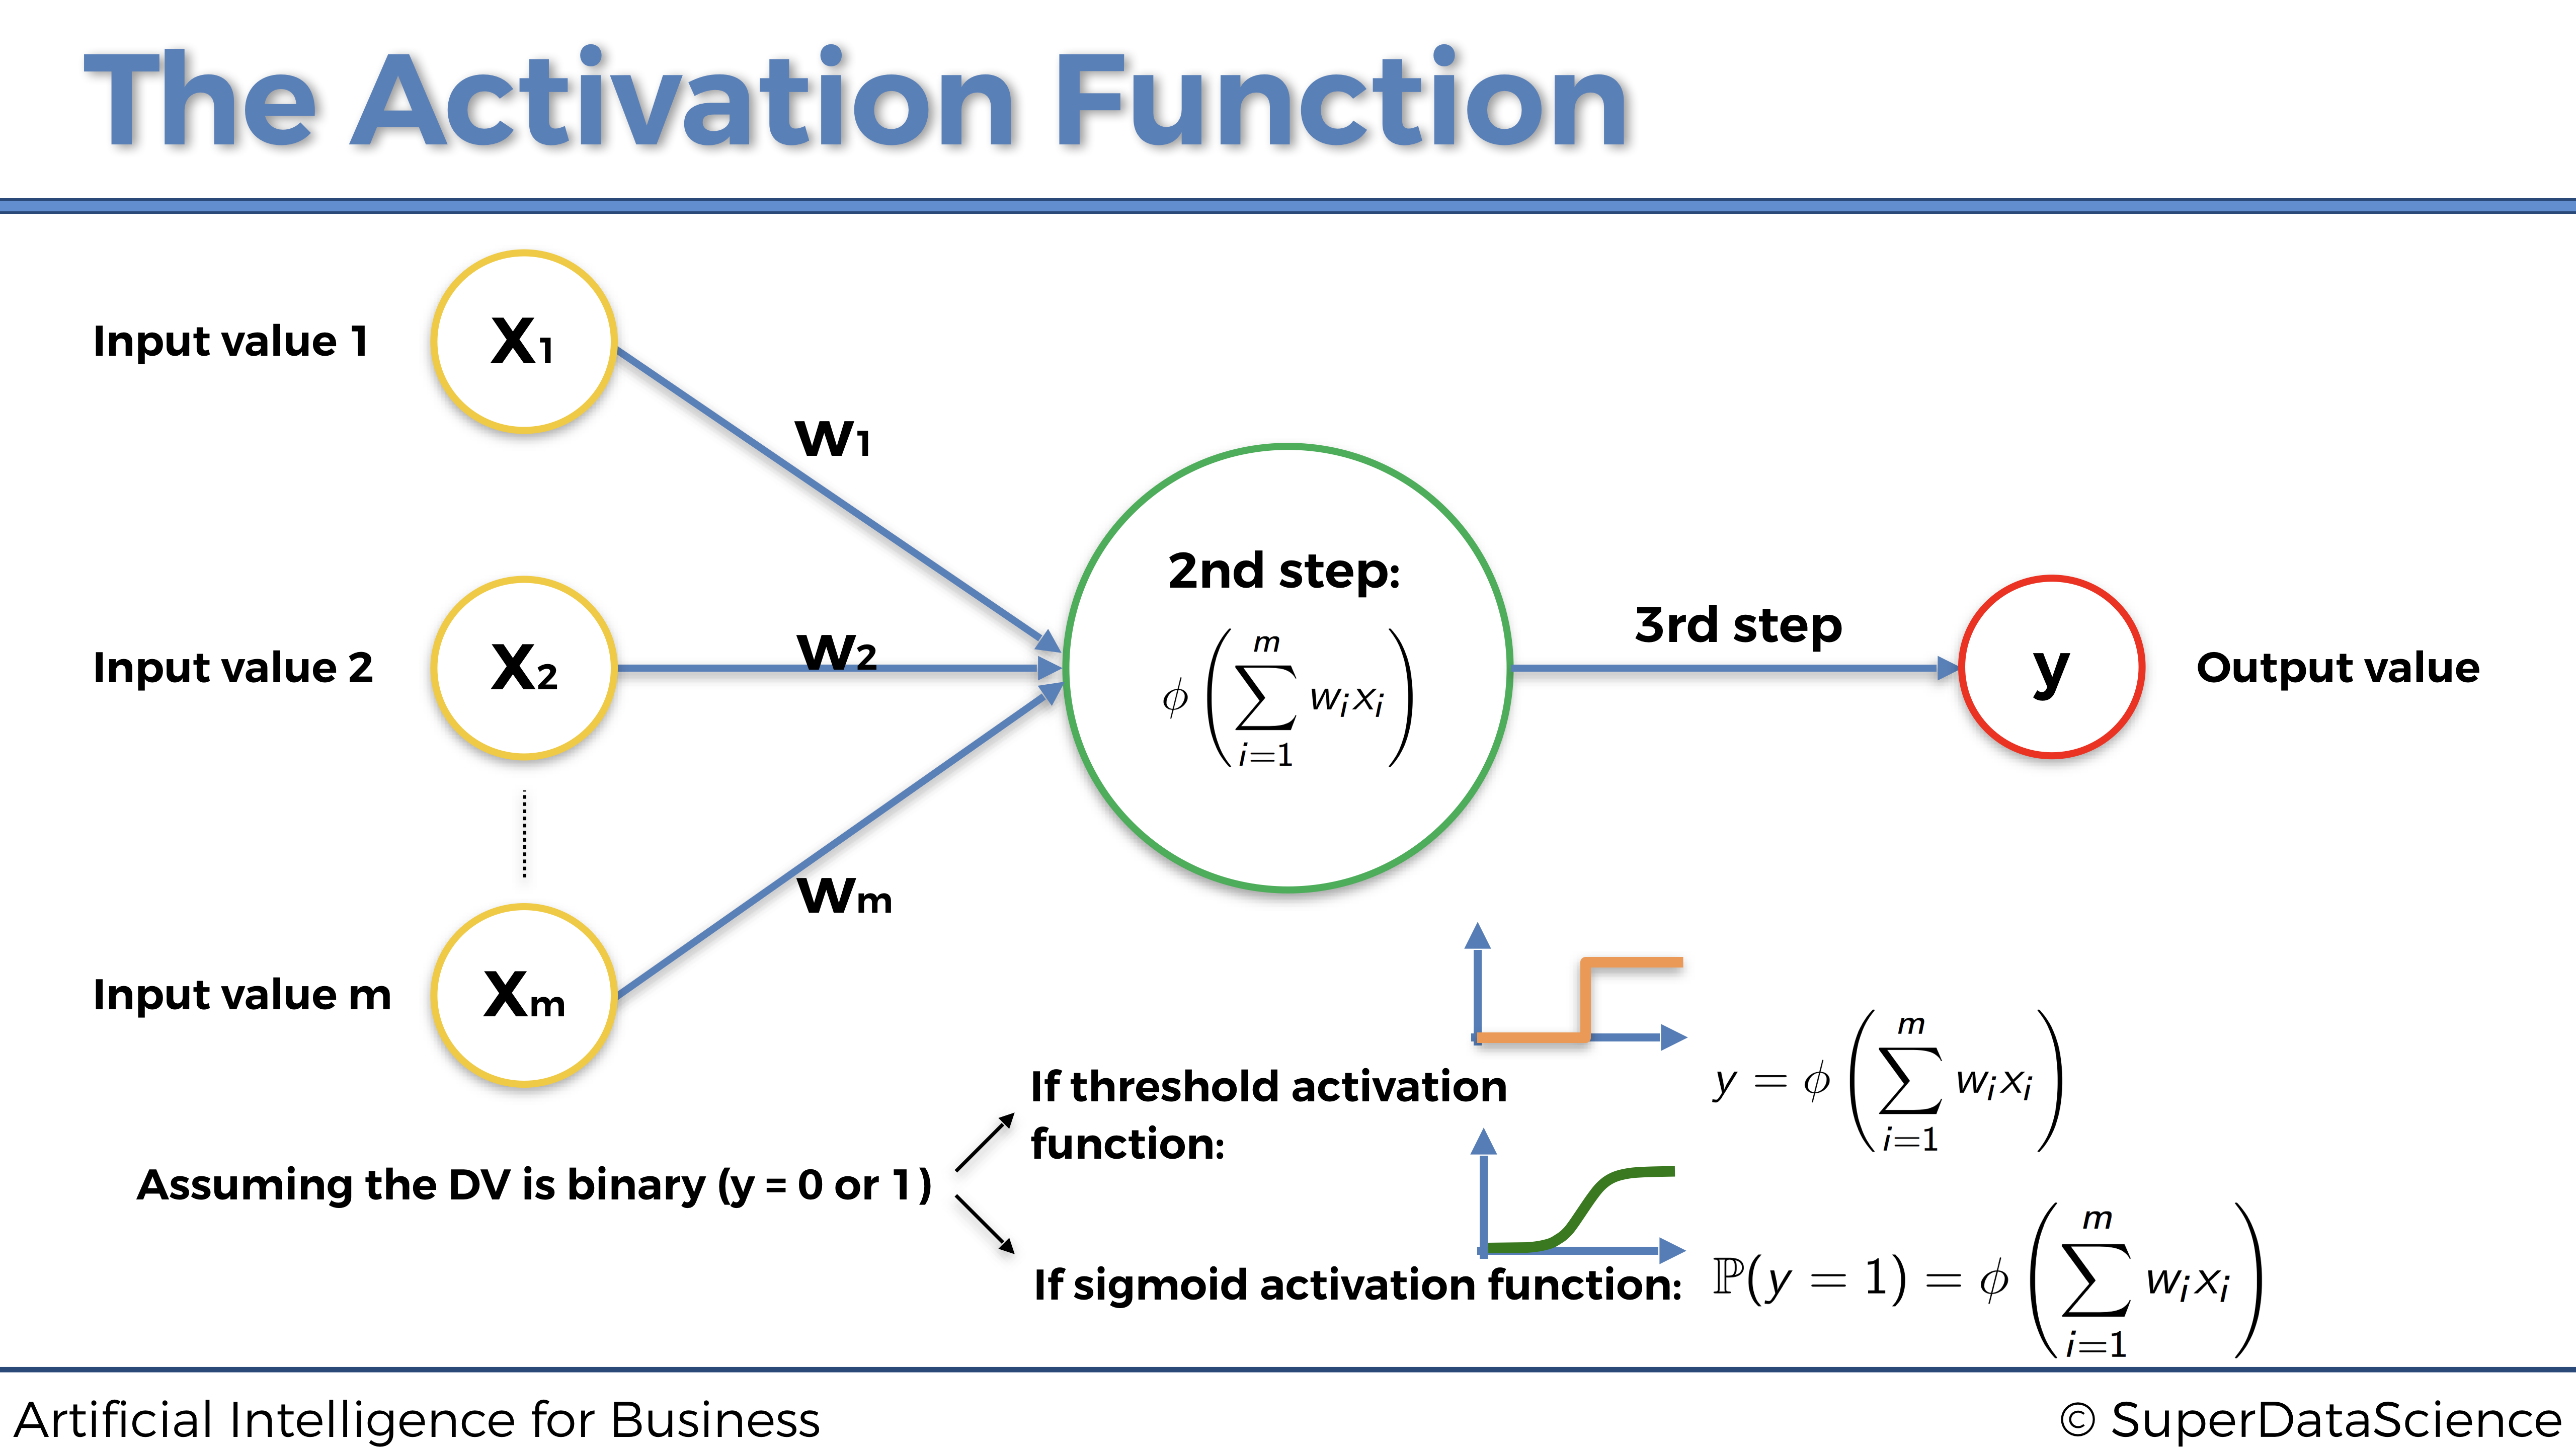
\includegraphics[scale=0.18]{ANN_14.png}
        \end{center}
\end{figure}

But then when should I use the other two activation functions, i.e.~the Rectifier activation function and the Hyperbolic Tangent activation function?

Easy again, the Rectifier and the Hyperbolic Tangent activation functions should be used within the hidden layers of a Deep Neural Network (with more than one hidden layer), except the last hidden layer leading to the output layer for which it is recommended to use a Sigmoid Activation function.

\newpage

Let's recap this again inside the following slide:

\begin{figure}[!htbp]
        \begin{center}
            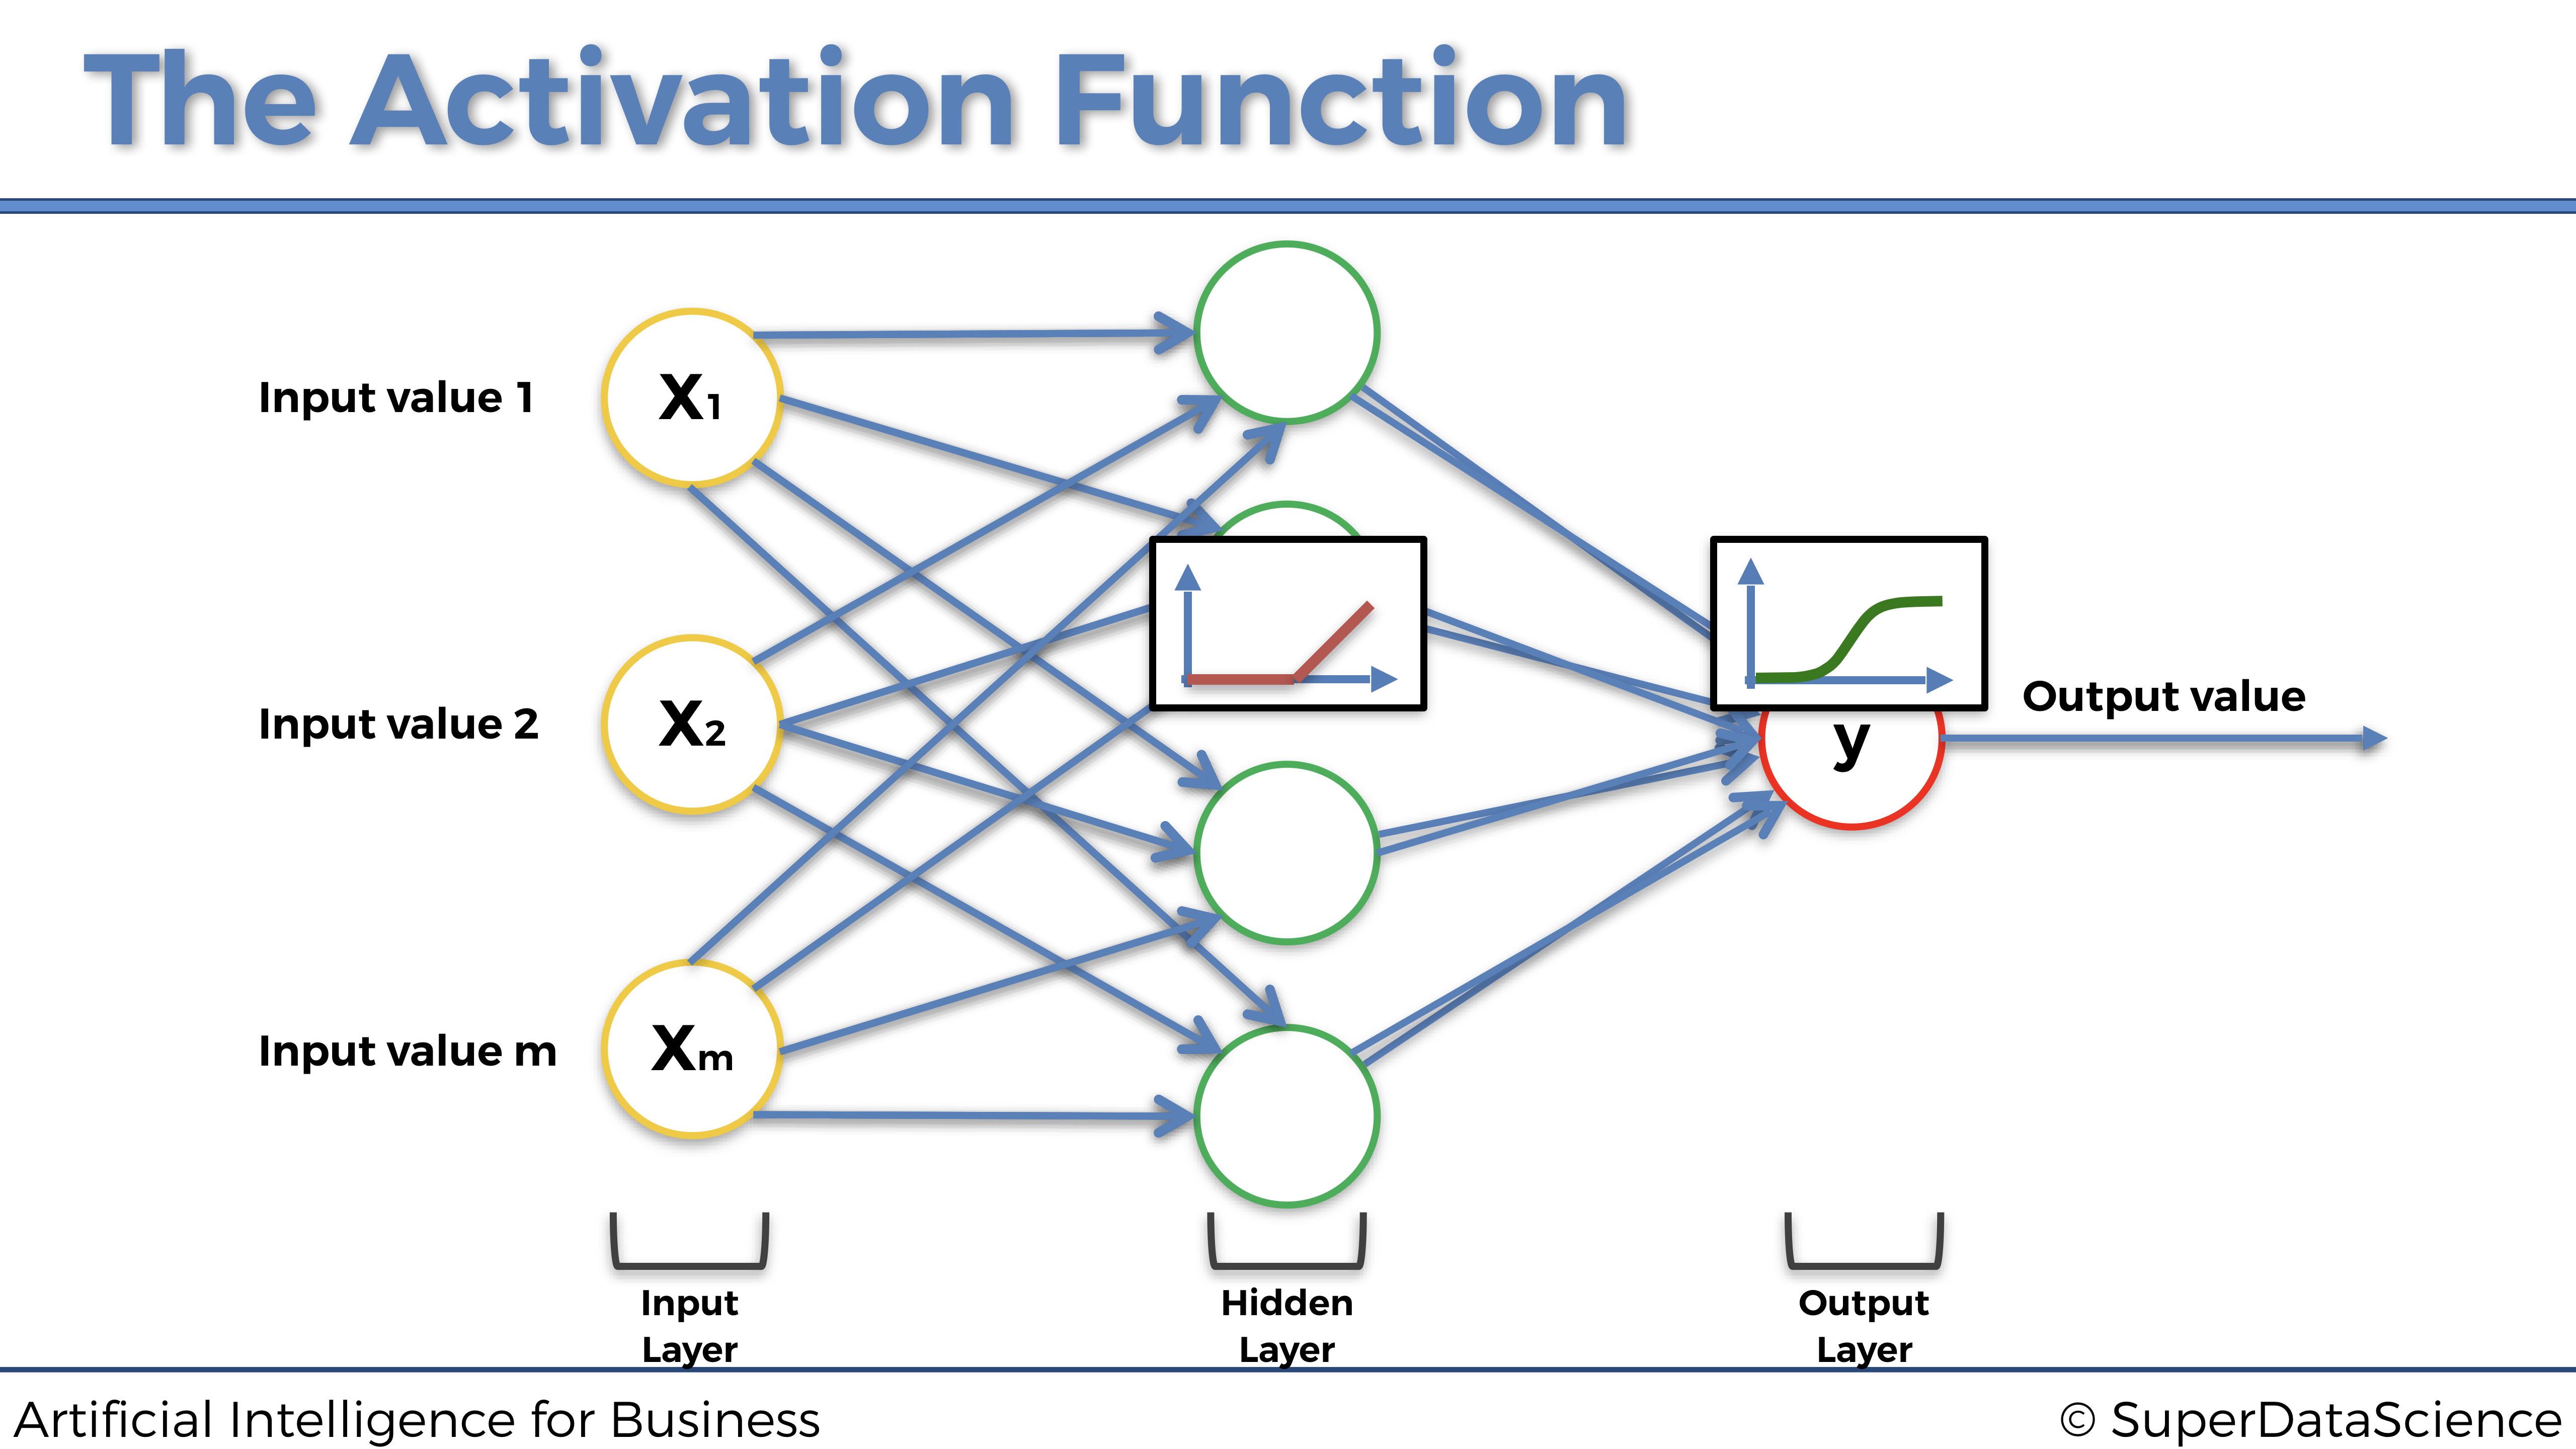
\includegraphics[scale=0.18]{ANN_15.png}
        \end{center}
\end{figure}

And lastly, how to choose between the Rectifier activation function and the Hyperbolic Tangent activation function in the hidden layers? Still easy, you should consider using the Rectifier activation function when the inputs are normalized (scaled between 0 and 1), and the Hyperbolic Tangent activation function when the inputs are standardized (scaled between -1 and +1):

\begin{figure}[!htbp]
        \begin{center}
            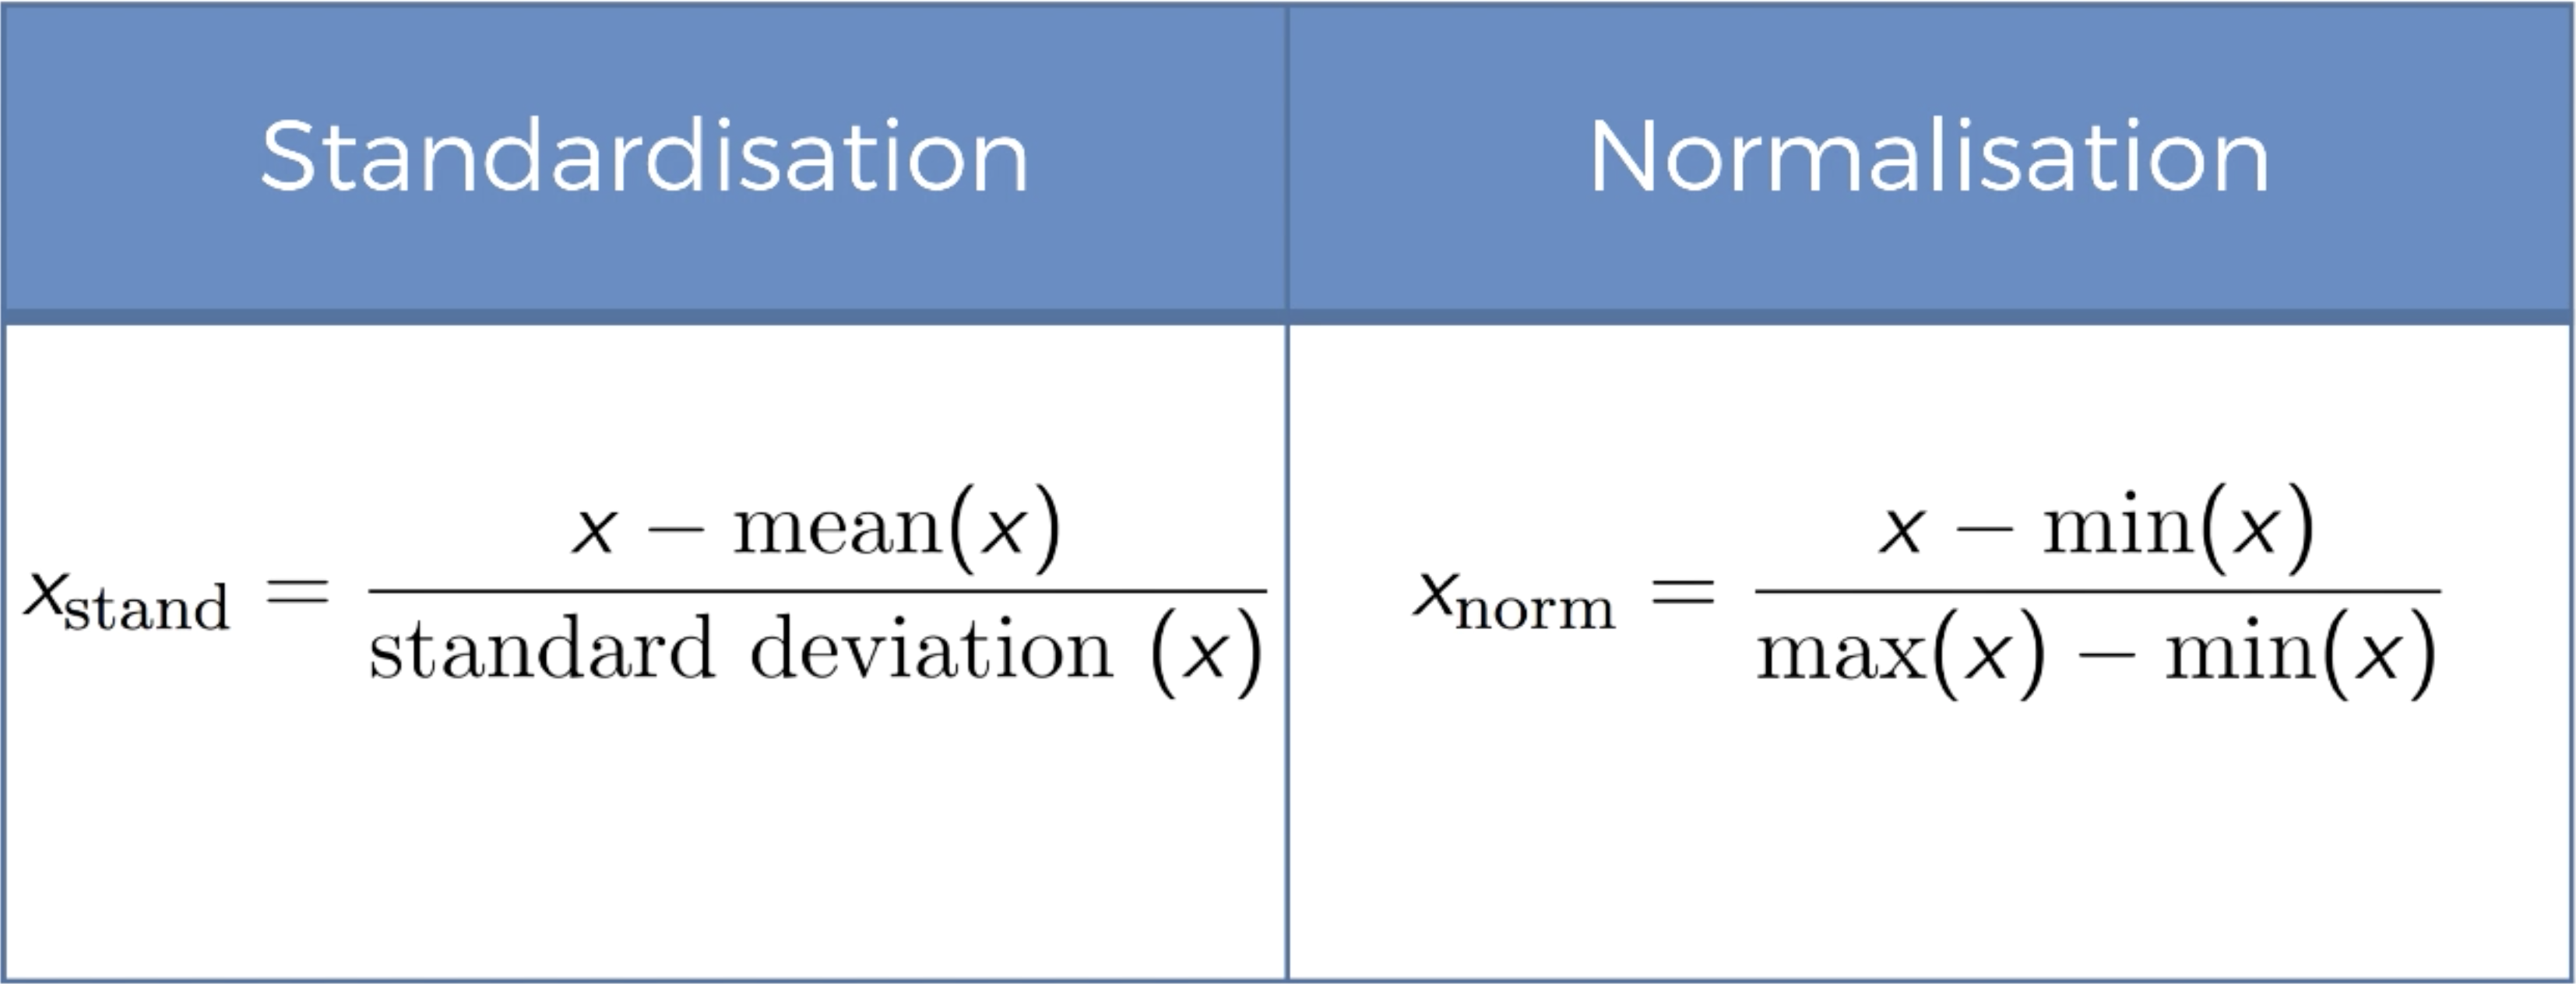
\includegraphics[scale=0.18]{ANN_16.png}
        \end{center}
\end{figure}

Now let's move on to the next section to explain, how Neural Networks work.

\newpage

\subsection{How do Neural Networks work?}

To explain this, let's consider the problem of predicting Real Estate prices. We have some independent variables which we are going to use to predict the price of houses and apartments. For simplicity purpose, and to be able to represent everything in a graph, let's say that our independent variables (our predictors) are the following:

\begin{enumerate}
    \item Area (squared feet)
    \item Number of Bedrooms
    \item Distance to city (Miles)
    \item Age
\end{enumerate}

Then, our dependent variable is of course the apartment price to predict.

Each of the independent variables is attributed a weight, in such a way that the higher is the weight, the more effect the independent variable will have on the dependent variable, that is, the stronger predictor it will be of the dependent variable. Hence, as soon as new inputs enter the Neural Network, the signals are forward-propagated from each of the inputs, reaching the neurons of the hidden layer. Then inside each neuron of the hidden layer, the activation function is applied, so that the lower is the weight of the input, the more the activation function will block the signal coming from that input, and the higher is the weight of that input, the more the activation will let that signal go through. And finally, all the signals coming from the hidden neurons, more or less blocked by the activation functions, are forward propagated to the output layer, to return the final outcome, that is the price prediction.

Let's represent this in the following graphic:

\begin{figure}[!htbp]
        \begin{center}
            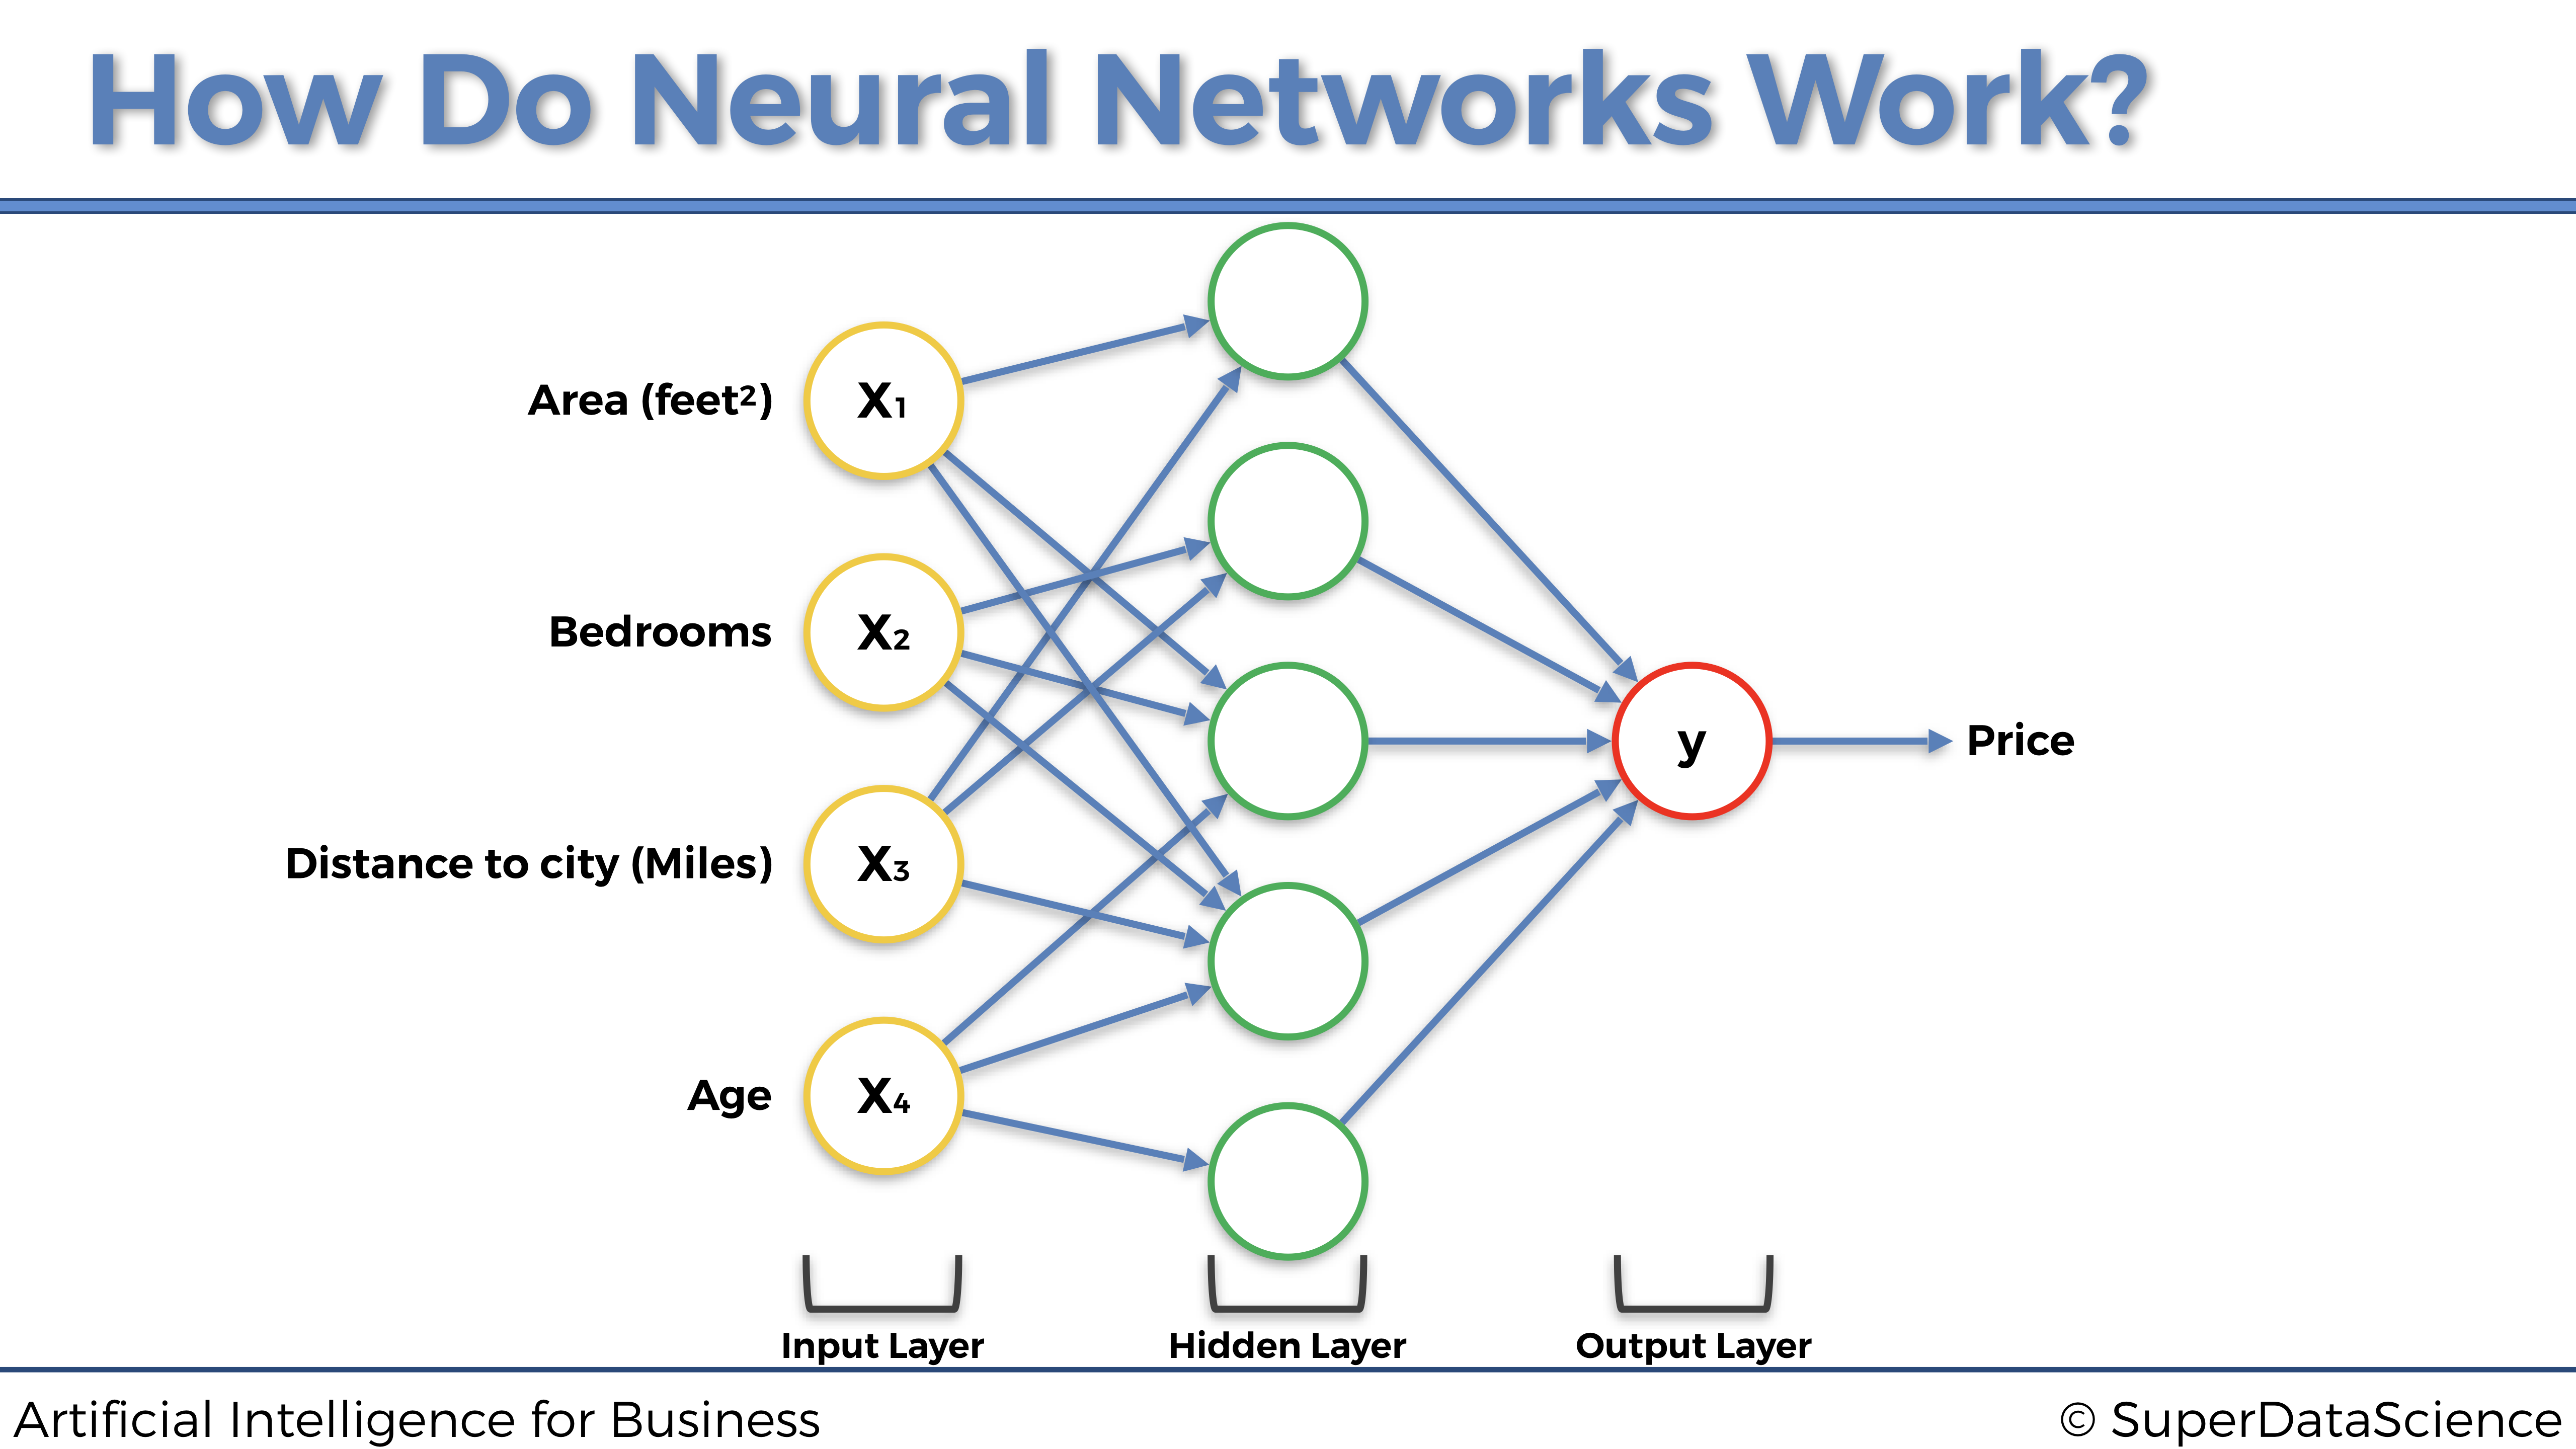
\includegraphics[scale=0.18]{ANN_17.png}
        \end{center}
\end{figure}

\newpage

\subsection{How do Neural Networks learn?}

Simply put, Neural Networks learn by updating, over many iterations, the weights of all the inputs and hidden neurons (when having several hidden layers), towards always the same goal to reduce the loss error between the predictions and the real values.

Indeed, in order for Neural Networks to learn, we need the actual values, which are also called the targets. In our example above about Real Estate Pricing, the actual values are the real prices of the houses and apartments in sales. These real prices depend on the independent variables listed above (area, number of bedrooms, distance to city, and age), and the Neural Network will learn to make better predictions of these prices, by running the following process:

\begin{enumerate}
    \item The Neural Network first forward propagates the signals coming from the input independent variables $x_1$, $x_2$, $x_3$ and $x_4$.
    
    \
    
    \item Then it gets the predicted price $\hat{y}$ in the output layer.
    
    \
    
    \item Then it computes the loss error $C$ between the predicted price $\hat{y}$ (prediction) and the actual price $y$ (target):
    
    \
    
    \begin{equation*}
        C = \frac{1}{2} (\hat{y} - y)^2
    \end{equation*}
    
    \
    
    \item Then this loss error is back-propagated inside the Neural Network, from right to left in our representation.
    
    \
    
    \item Then on each of the neurons the Neural Network runs a technique called Gradient Descent (which we will discuss in the next section), to update the weights into the direction of loss reduction, that is, into new weights which reduce the loss error $C$.
    
    \
    
    \item Then this whole process is repeated many times, with each time new inputs and new targets, until we get the desired performance (early stopping) or the last iteration (number of iterations chosen in the implementation).
\end{enumerate}

Let's represent the two main phases, forward-propagation and back-propagation, of this whole process in the two following separate graphics (see next page):

\newpage

\subsection{Forward-Propagation and Back-Propagation}

\textbf{Phase 1: Forward-Propagation:}

\begin{figure}[!htbp]
        \begin{center}
            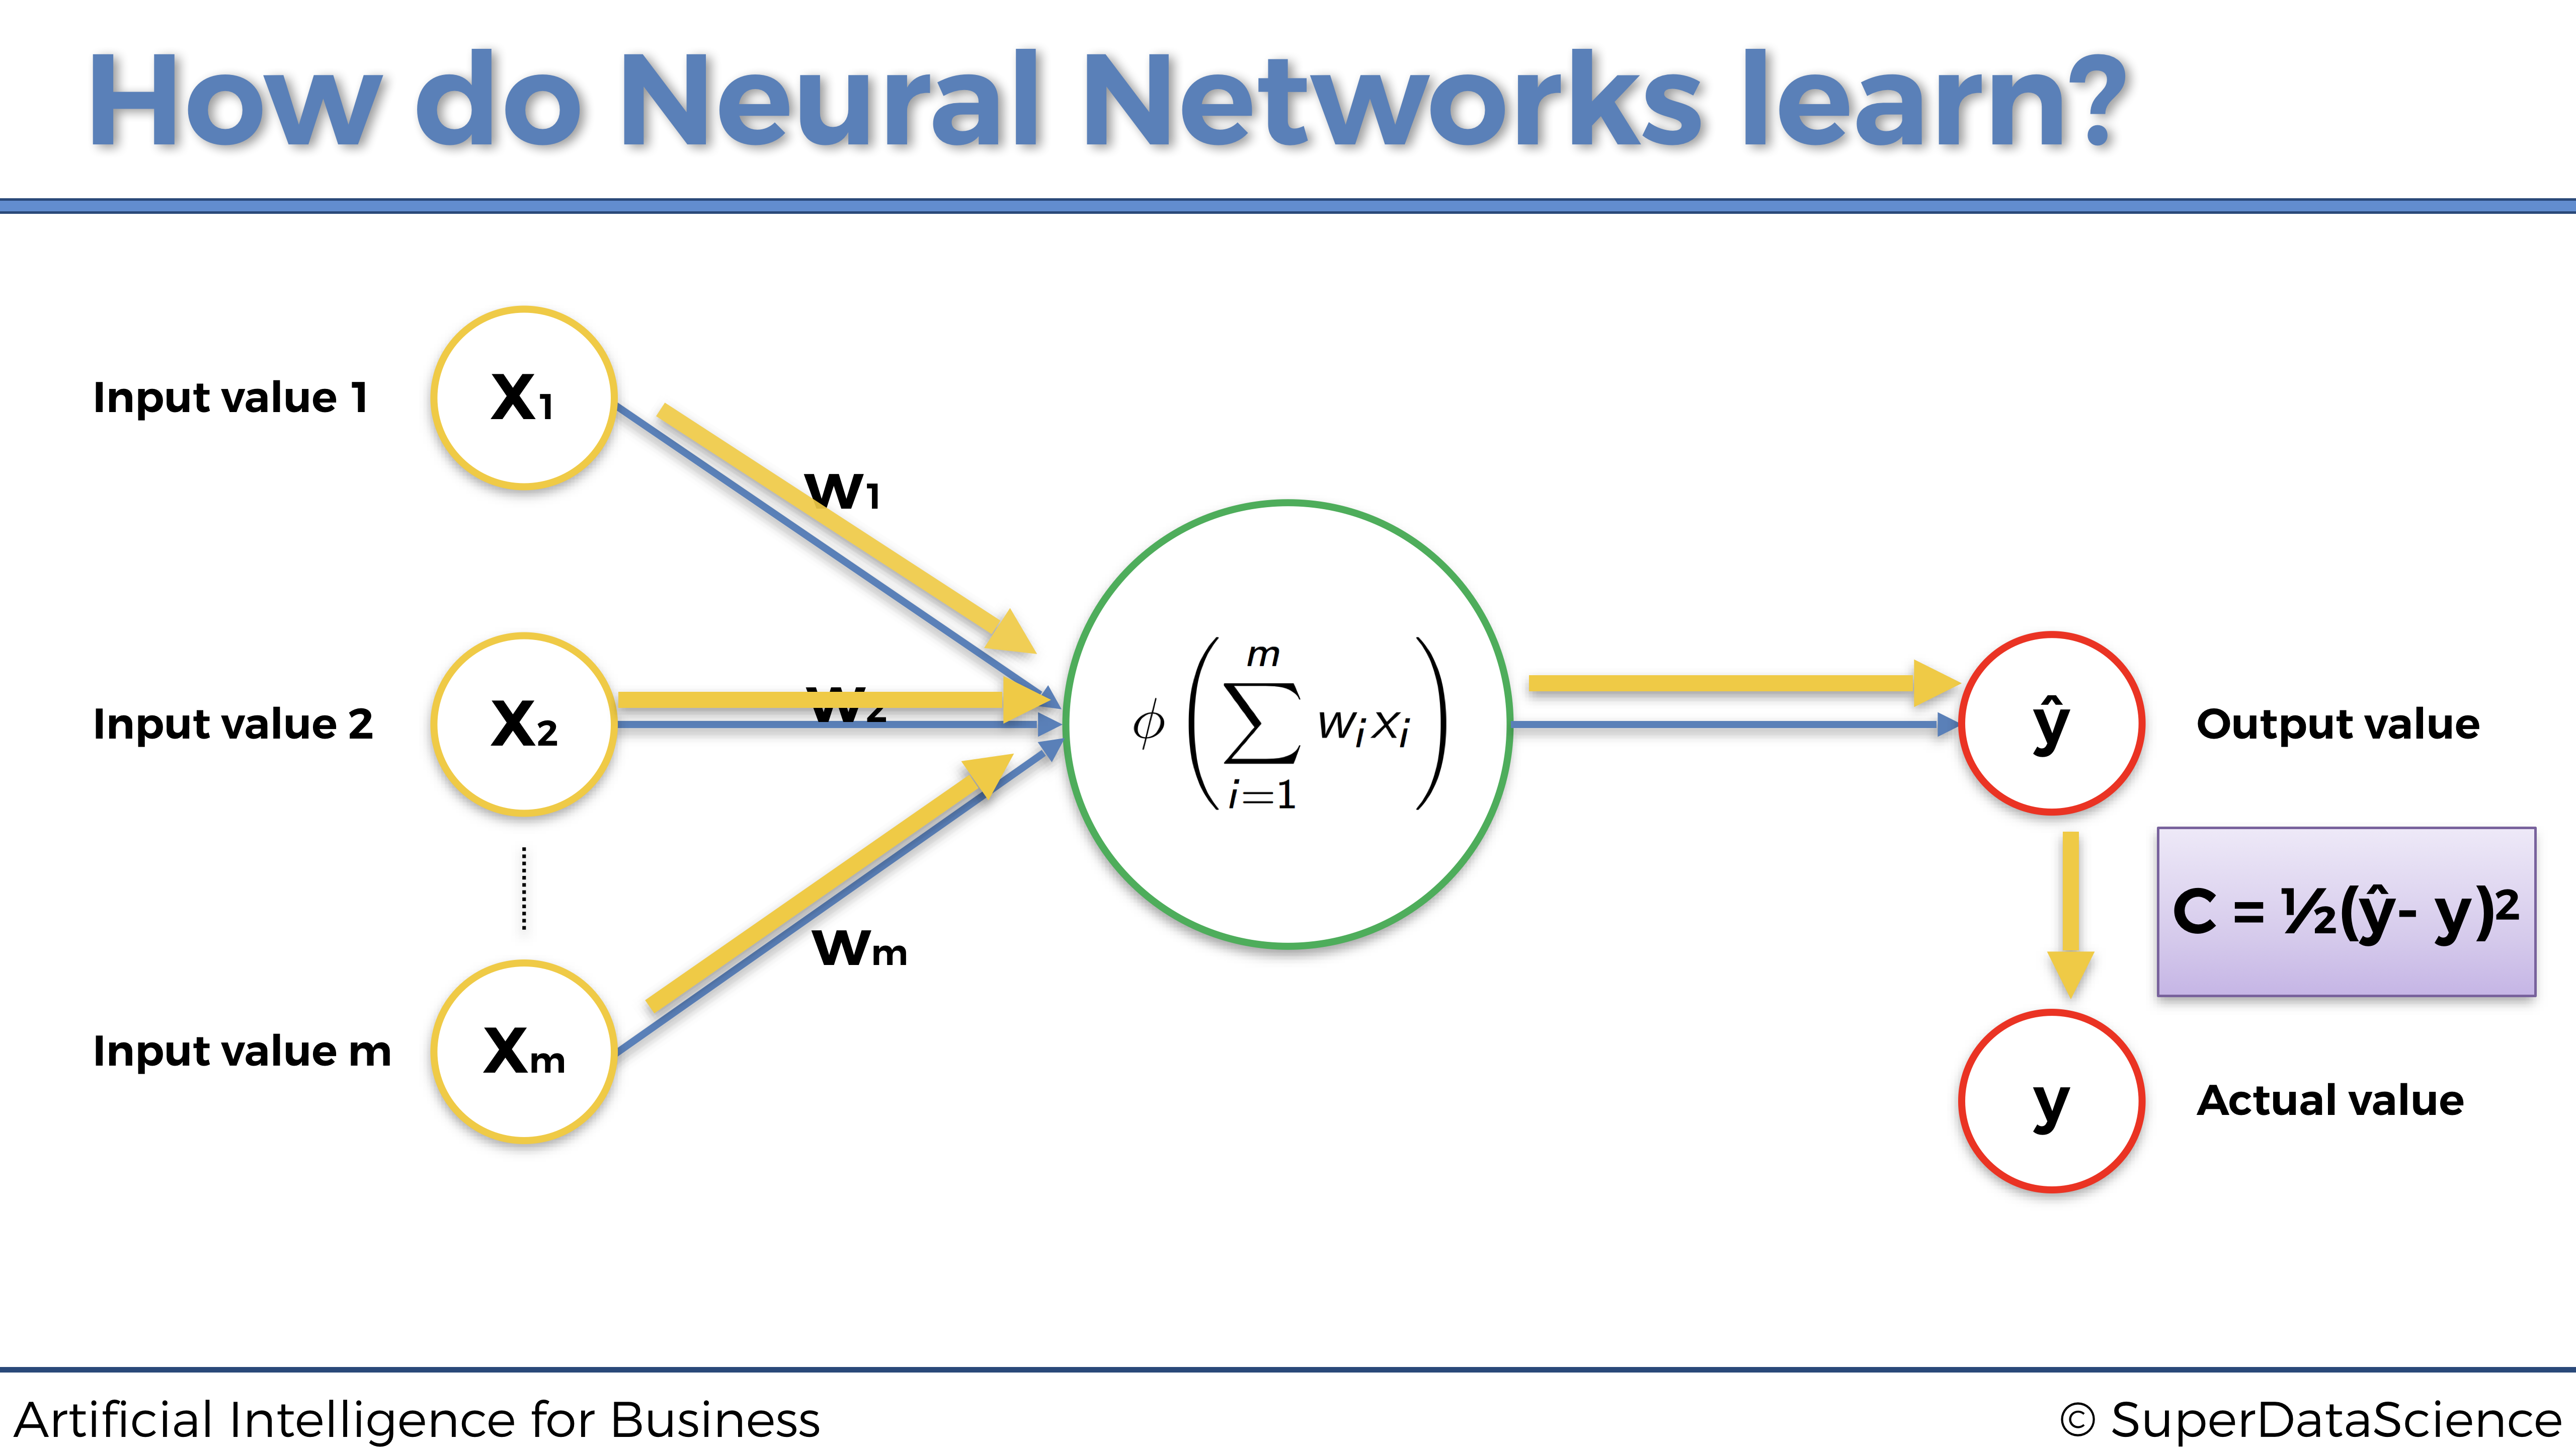
\includegraphics[scale=0.18]{ANN_18.png}
        \end{center}
\end{figure}

\textbf{Phase 2: Back-Propagation:}

\begin{figure}[!htbp]
        \begin{center}
            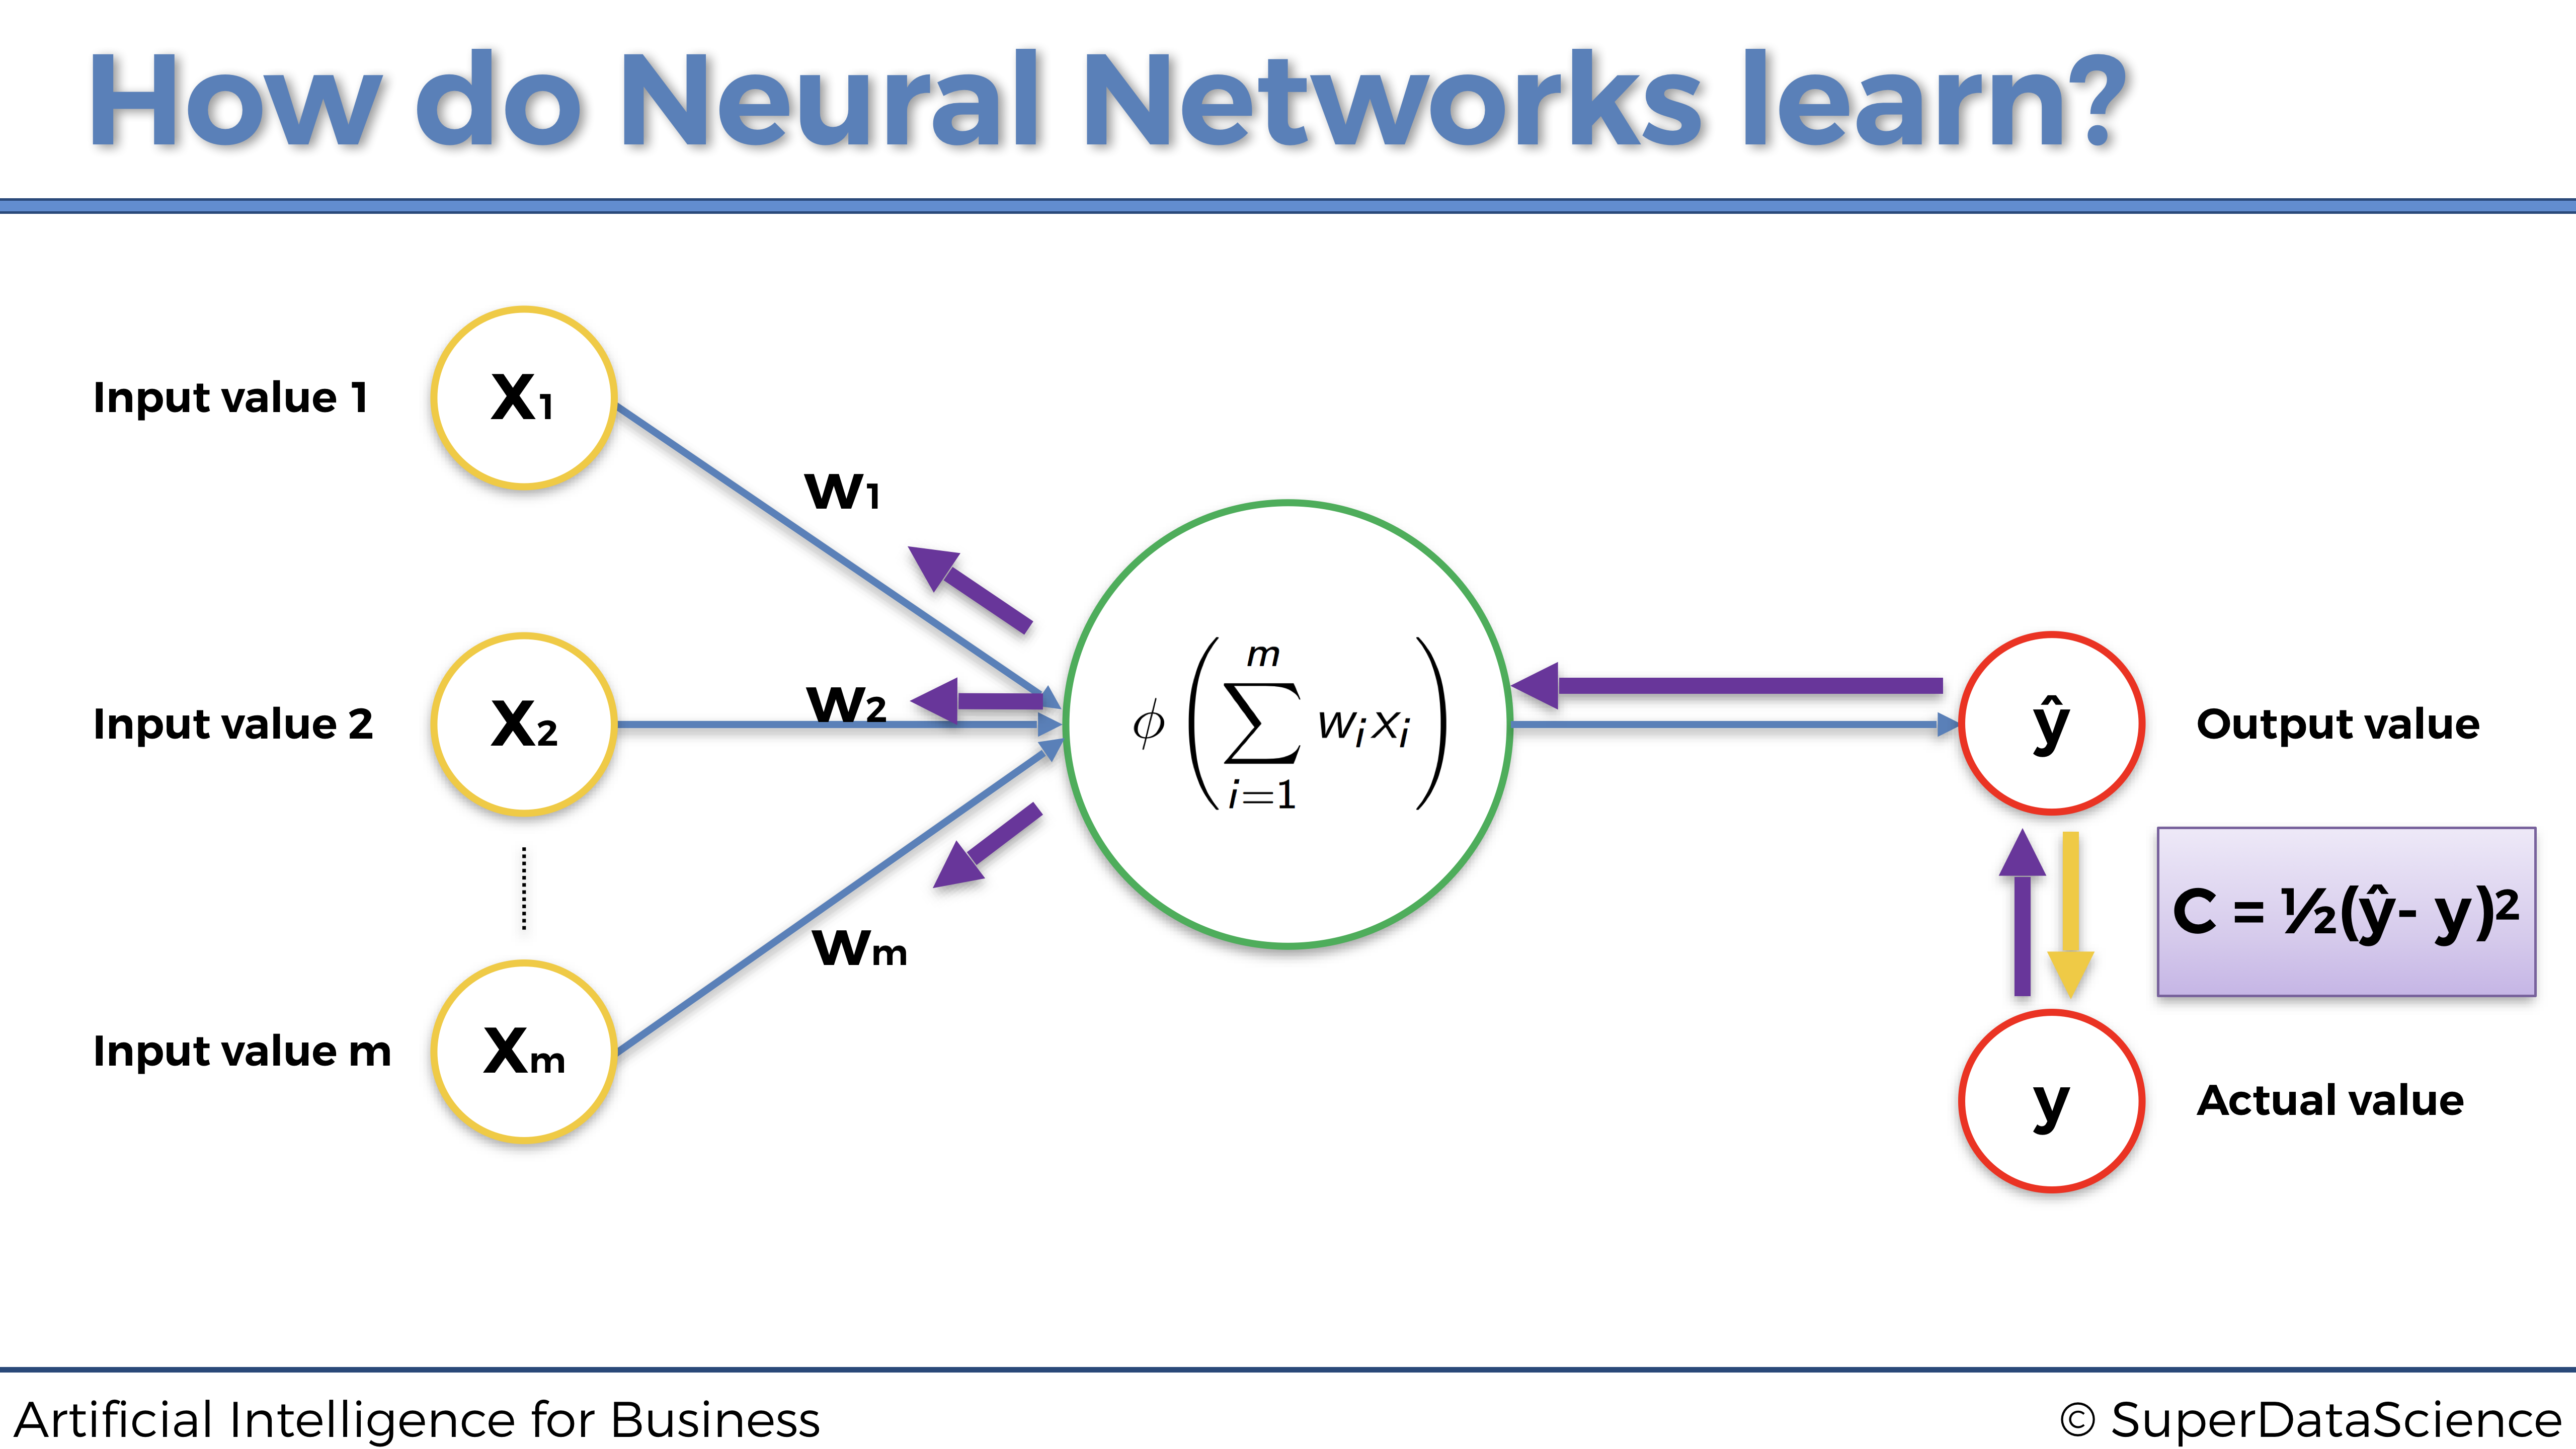
\includegraphics[scale=0.18]{ANN_19.png}
        \end{center}
\end{figure}

\newpage

\subsection{Gradient Descent}

\subsubsection{Gradient Descent Introduction}

When people talk about Machine Learning or Deep Learning they mostly talk about algorithms that are used. But the real questions are, why are those algorithms considered to be Machine Learning or Deep Learning algorithms and others are not? What is the underlining technique that connects them?

The answer to the first question is pretty intuitive: those algorithms are considered to learn their parameters by themselves. This property was not very common before and most algorithms were hand tuned by engineers to achieve a required specification/goal.

But then Gradient Descent came on stage and most algorithms that did not work before suddenly made sense and started to optimize themselves.

So is Gradient Descent magic? Well to someone it is, but for us it is a mathematical algorithm that is used to optimize a model that has its internal parameters (weights). Or, to be more technical, let's see what Wikipedia says about it:

\begin{center}
    “Gradient descent is a first-order iterative optimization algorithm for finding the minimum of a function.”
\end{center}

That is a correct but mouthful definition, and for someone that is just starting, it is the scary one as well! Let's break it down:

\textbf{Algorithm} - In simple words, it is a blueprint on how to solve a problem. Everyday example of an algorithm would be a cooking recipe.

\textbf{Iterative} - This means that it uses some kind of loop (for programmers, for-loops or while-loops) to perform steps. Each step uses previously calculated values as an input for the current step. Now, one question rises, ``What is our initial value?''. We will answer on this a bit later through examples.

\textbf{Optimization} - It tries to find the best solutions according to some criteria leading to several alternative solutions, but only one is consider the best.

\textbf{First-order} - Gradient Descent is using first derivative of a criterion function (cost, loss) in order to find what is a better solution to the given problem.

Hence, when we put everything together in simple words, we get the following:

Gradient descent is a blueprint on how to find the best solution to a problem where more than one solution is acceptable. It uses a goal to determine how far we are from finding the best solution.

Until this point we have everything clarified except the cost function.

The cost is the indicator that we follow during the optimization process. Based on that indicator we can tell how far we are from the optimum of a function. One good example of the Cost is the Mean-Squared Error, which we have seen earlier in this book:

\begin{equation*}
    \textrm{MSE} = \frac{1}{n} \sum_{i=1}^n (y_i - \hat{y}_i)
\end{equation*}

where:

\begin{equation*}
    \begin{cases}
        \textrm{$\hat{y}_i$ is the model prediction} \\
        \textrm{$y_i$ is the target (the actual value)} \\
        \textrm{$n$ is the number of samples in a dataset}
    \end{cases}
\end{equation*}

Every algorithm that uses Gradient Descent as an optimization technique has parameters (weights) which are changing during the optimization process. When we say that we are looking for the minimum of the loss function, we actually mean we are looking for the values of the weights for which the loss has the lowest possible value.

Accordingly, to answer our second question from the beginning, the technique that connects all the Machine Learning algorithms from Linear Regression to the most complicated neural networks is indeed, Gradient Descent.

\subsubsection{Gradient Descent Intuition}

As we have seen, Gradient Descent is an optimization technique that helps us find the minimum of a cost function. Now let's visualize it in the most intuitive way, like the following ball in a bowl (with little math sprinkle on top of it):

\begin{figure}[!htbp]
        \begin{center}
            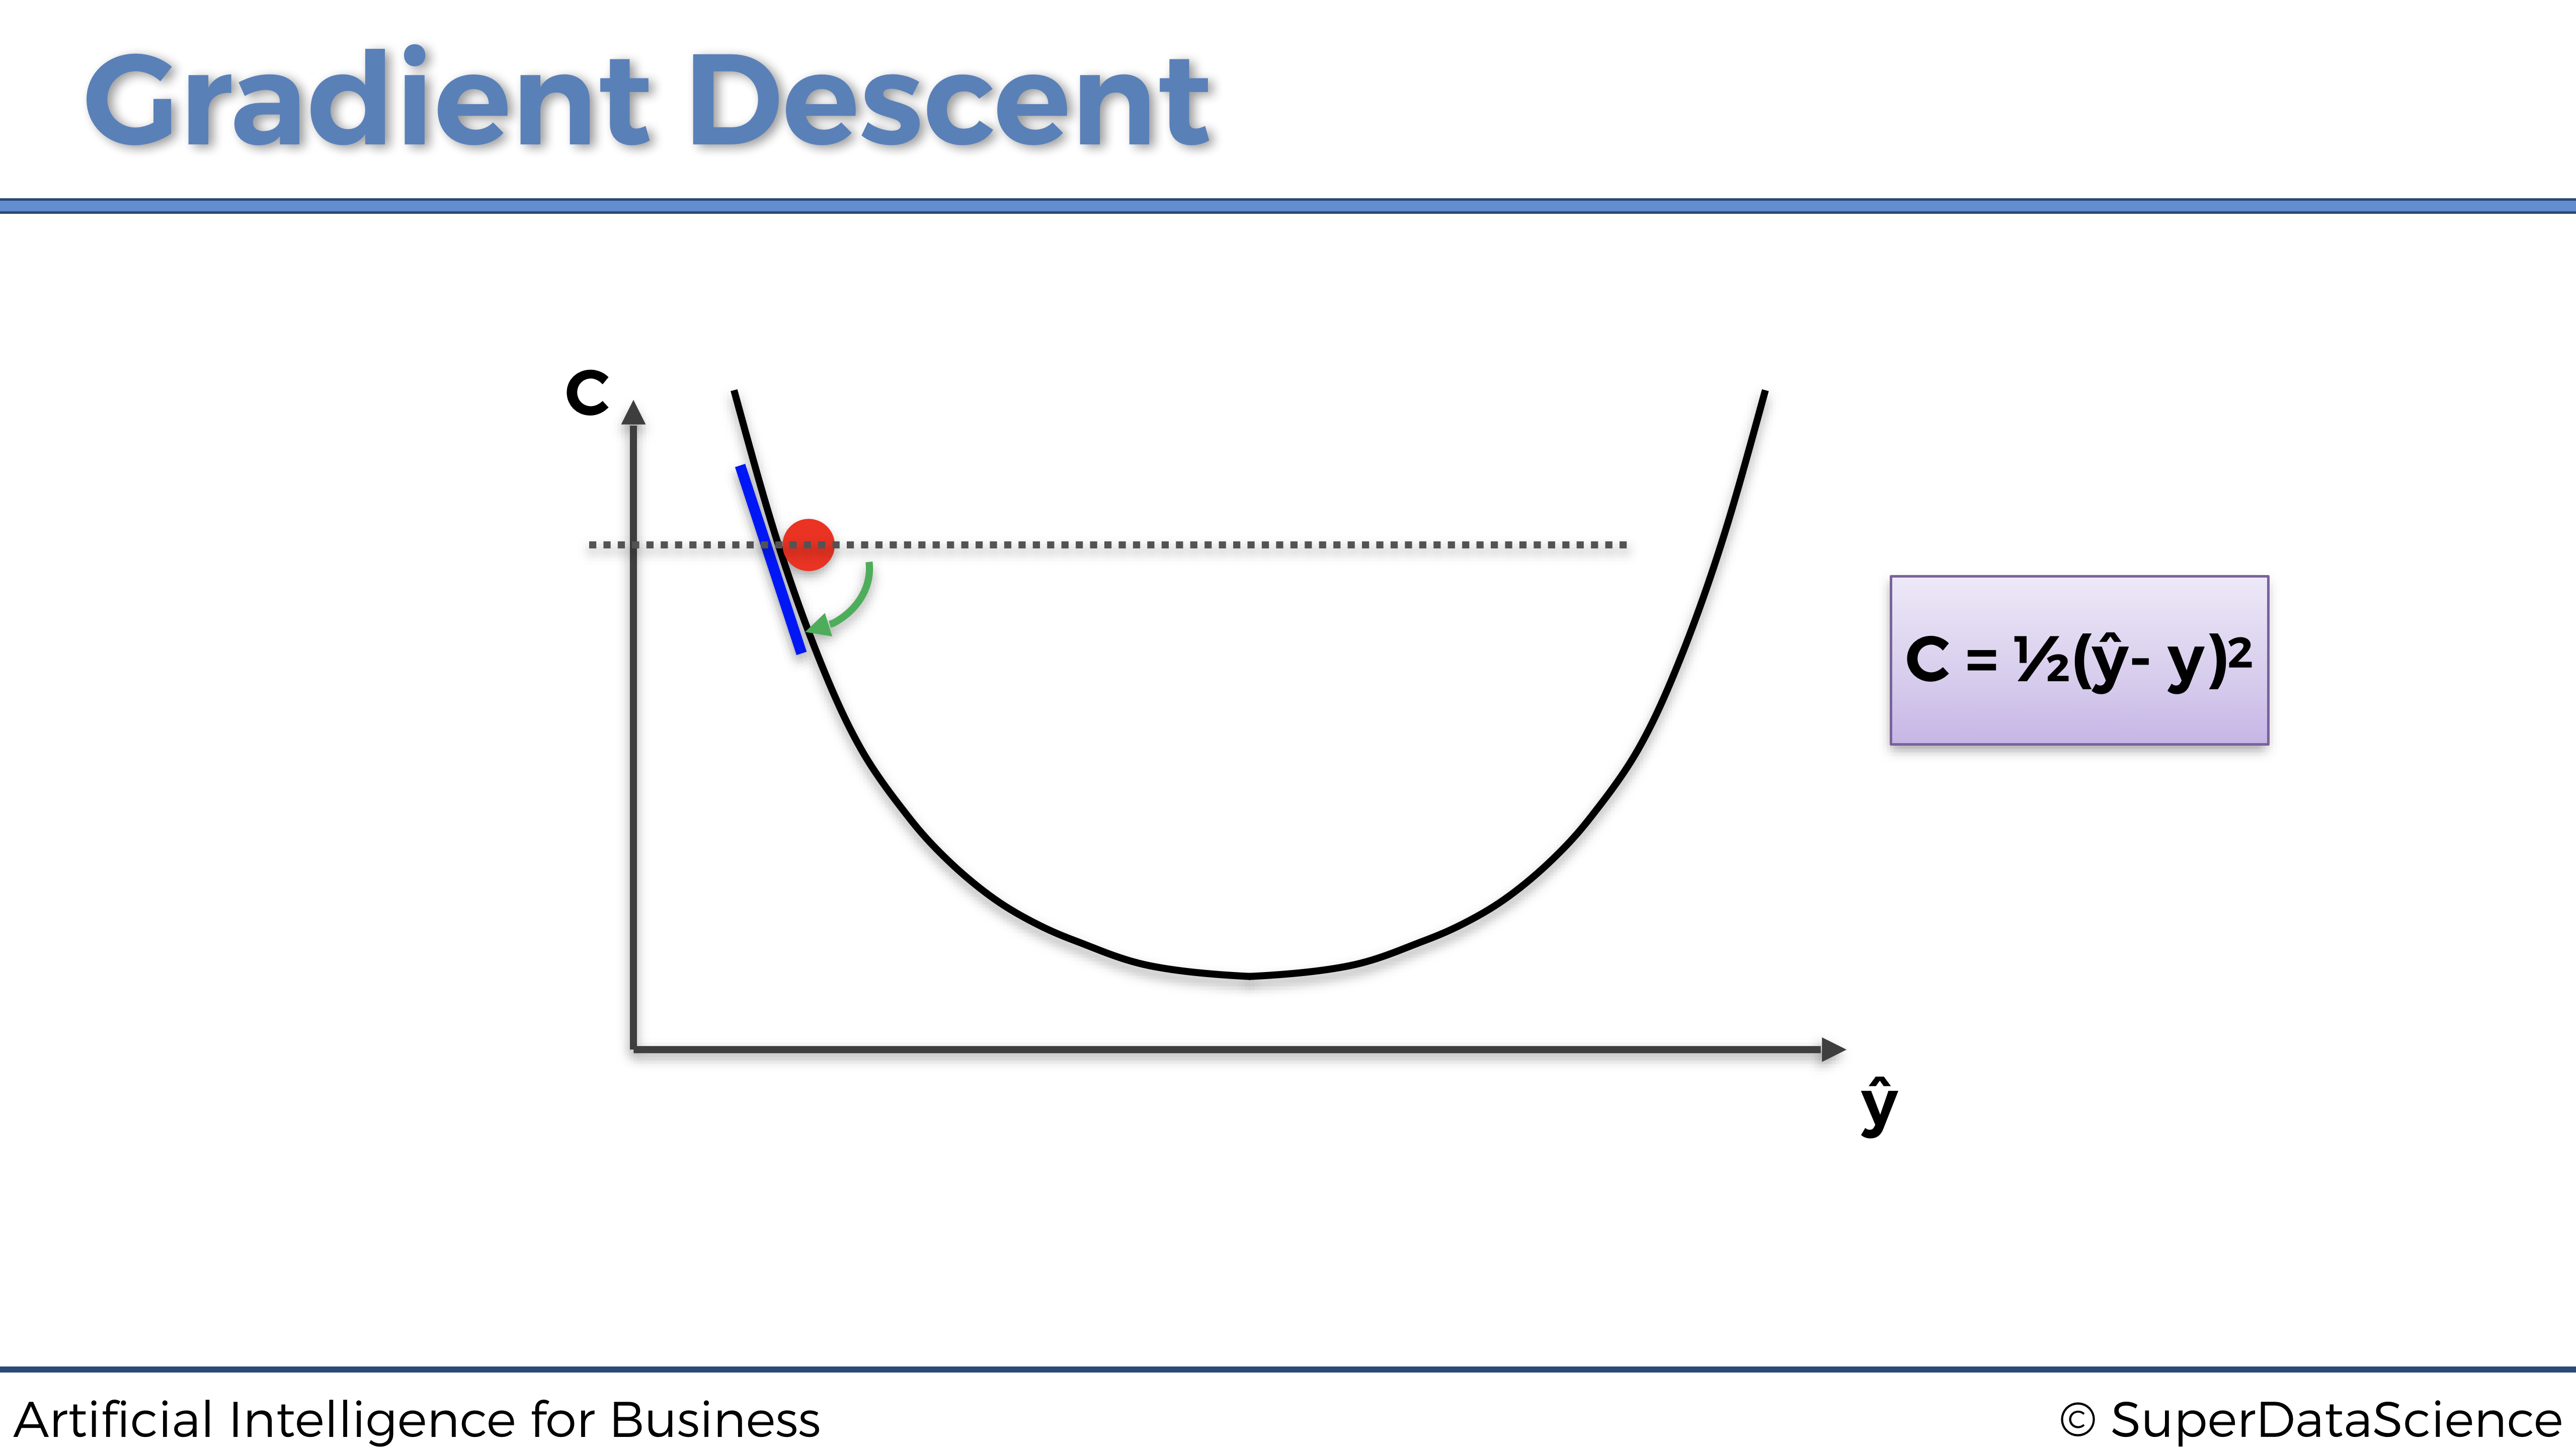
\includegraphics[scale=0.18]{ANN_20.png}
        \end{center}
\end{figure}

Imagine this is a cross section of a bowl, inside which we drop a small red ball and let it find its way down to the bottom of the bowl. After some time it will stop rolling since it has found the sweet spot for it, at the bottom of the bowl.

You can think about the Gradient Descent in the same way. It starts somewhere in the bowl (initial values of parameters) and tries to find the bottom of the bowl, or in other words, the minimum of a cost function.

Let's go through the example that is shown on the image above. The initial values of the parameters have set our ball at the position shown. Based on that we get some predictions, which we compare to our target values. The difference between these two sets will be our loss for the current set of parameters.

Then we calculate the first derivative of the cost function, with respect to the parameters. This is where the name \textbf{Gradient} comes from. Here, this first derivative gives us the slope of the tangent to the curve where the ball is. If the slope is negative, like on the picture above, we take the next step to the right side. If the slope is positive we take the next step to the left side.

The name \textbf{Descent} thus comes from the fact that we always take the next step that points downhill, as represented in the following graphic:

\begin{figure}[!htbp]
        \begin{center}
            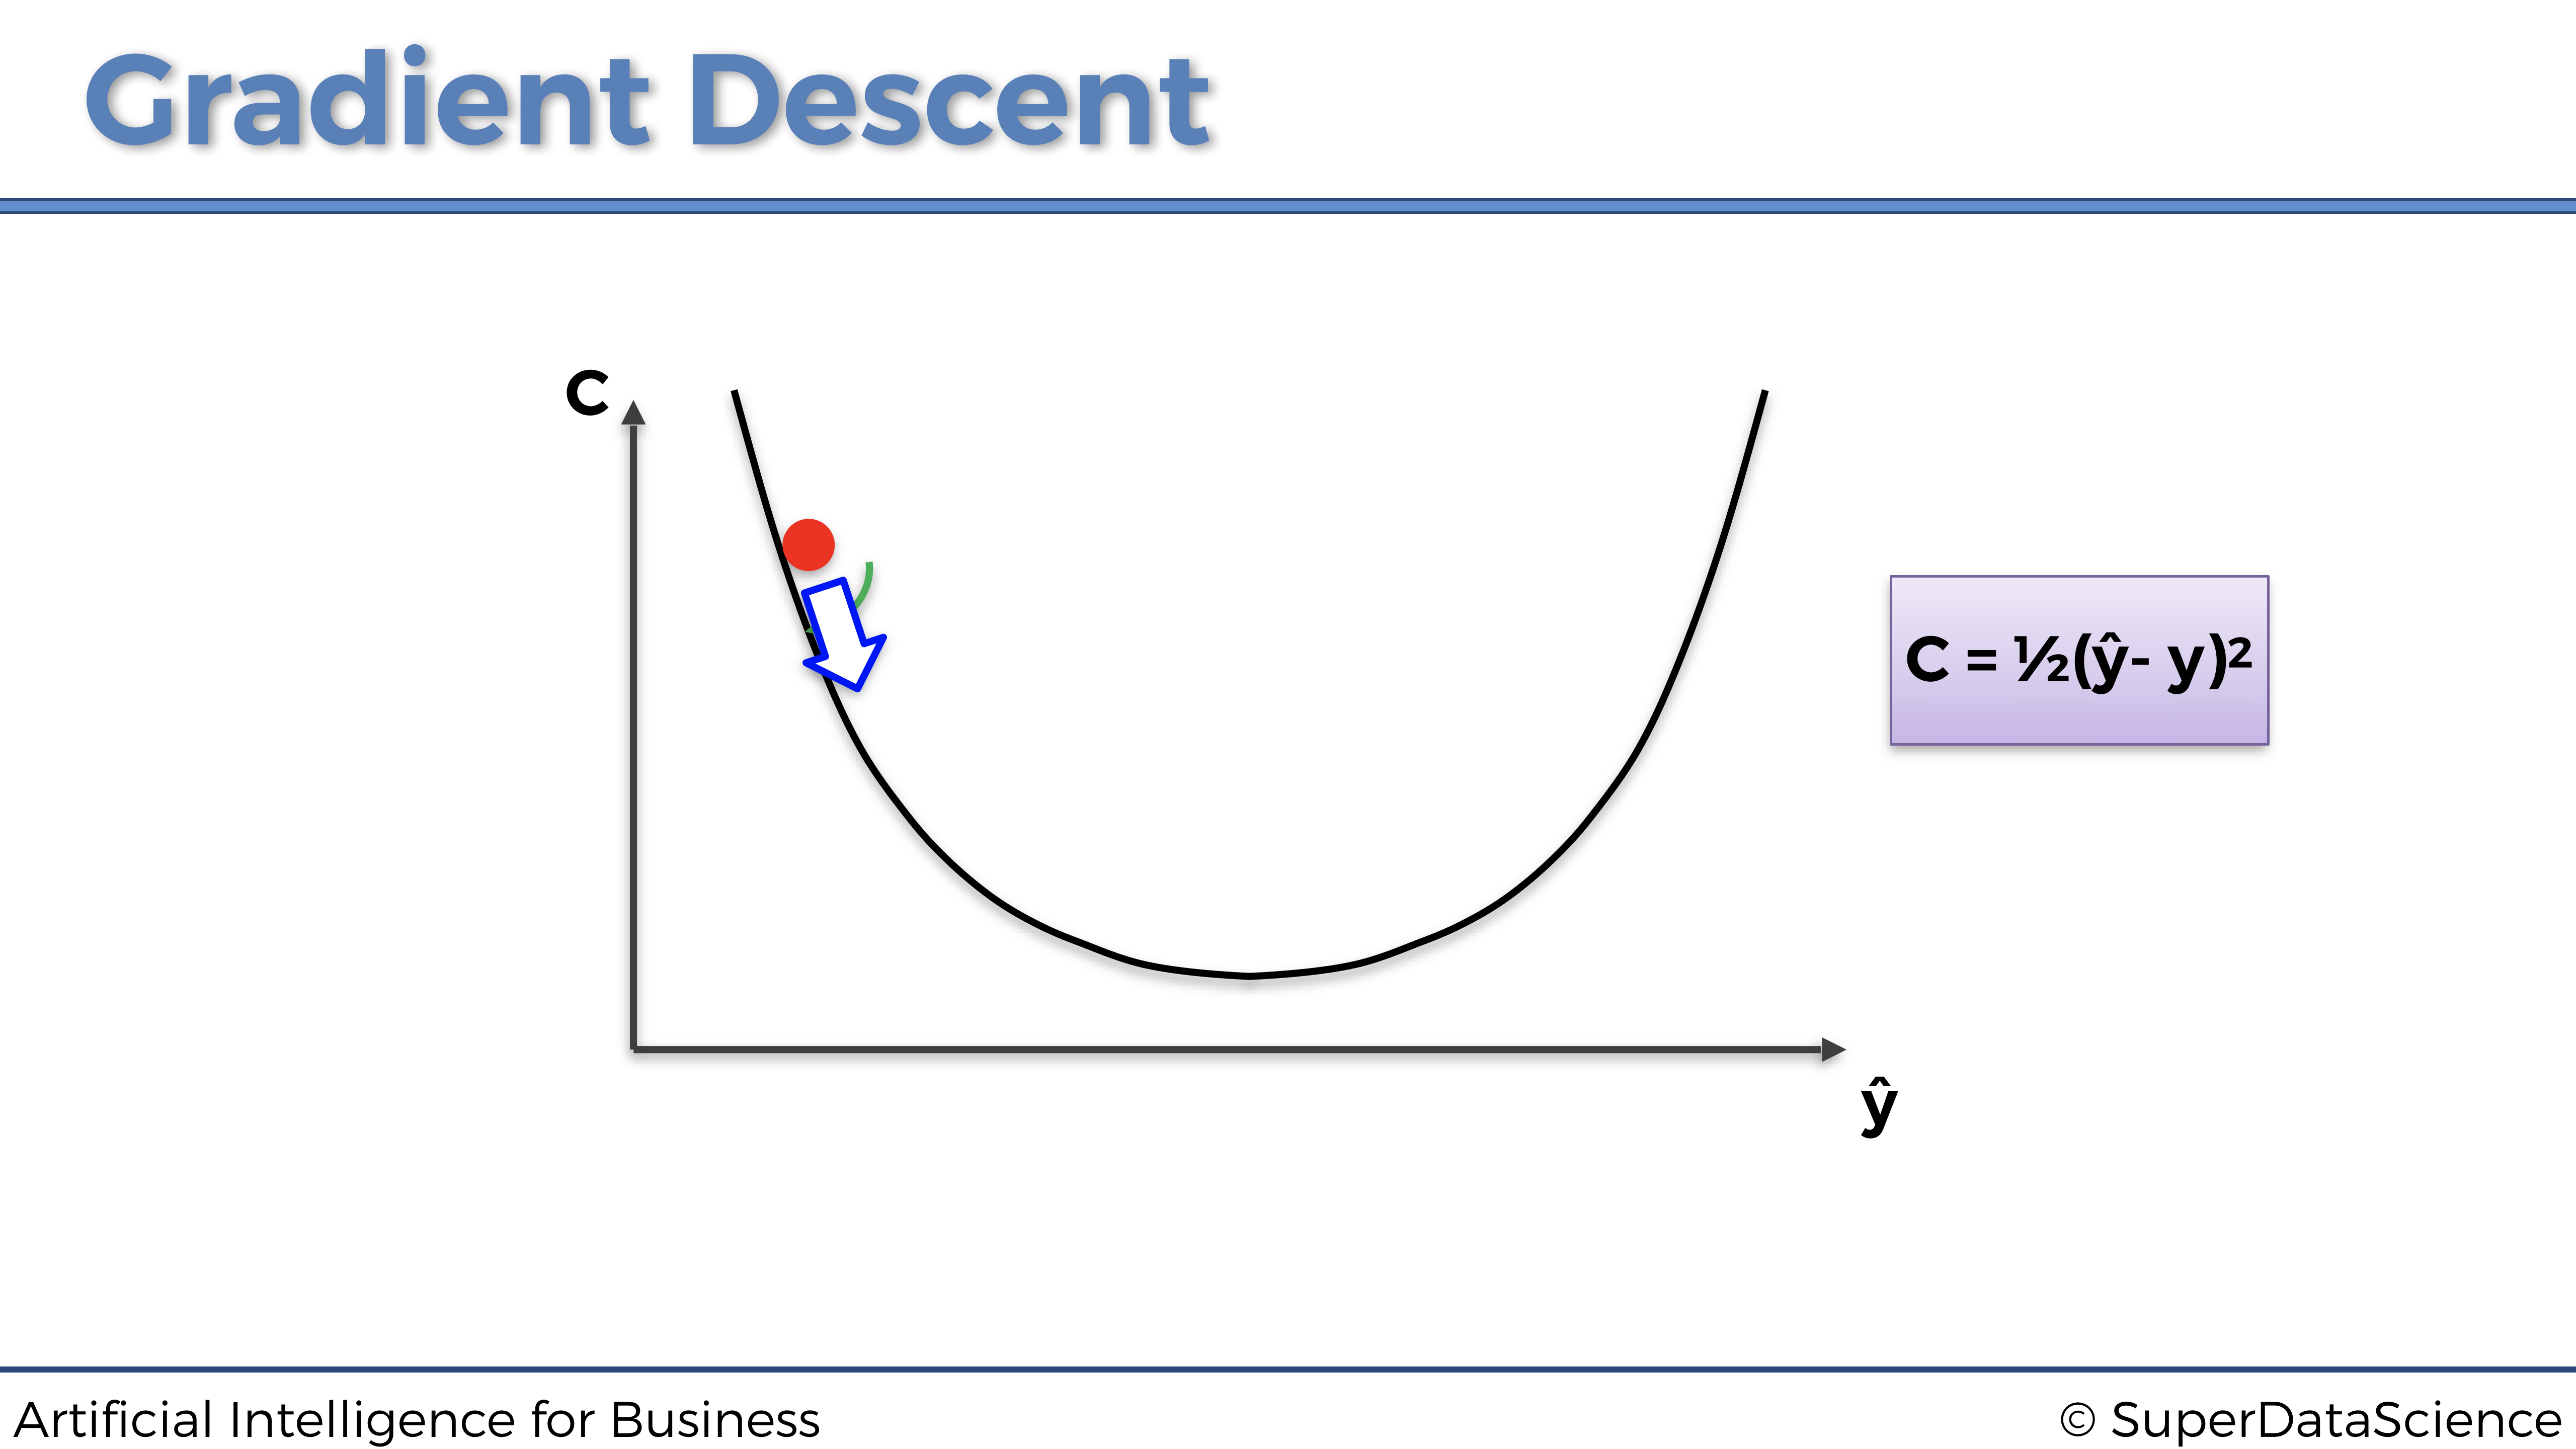
\includegraphics[scale=0.15]{ANN_21.png}
        \end{center}
\end{figure}

Now at this position our ball has a positive slope, so we have to take the next step to the left.

\begin{figure}[!htbp]
        \begin{center}
            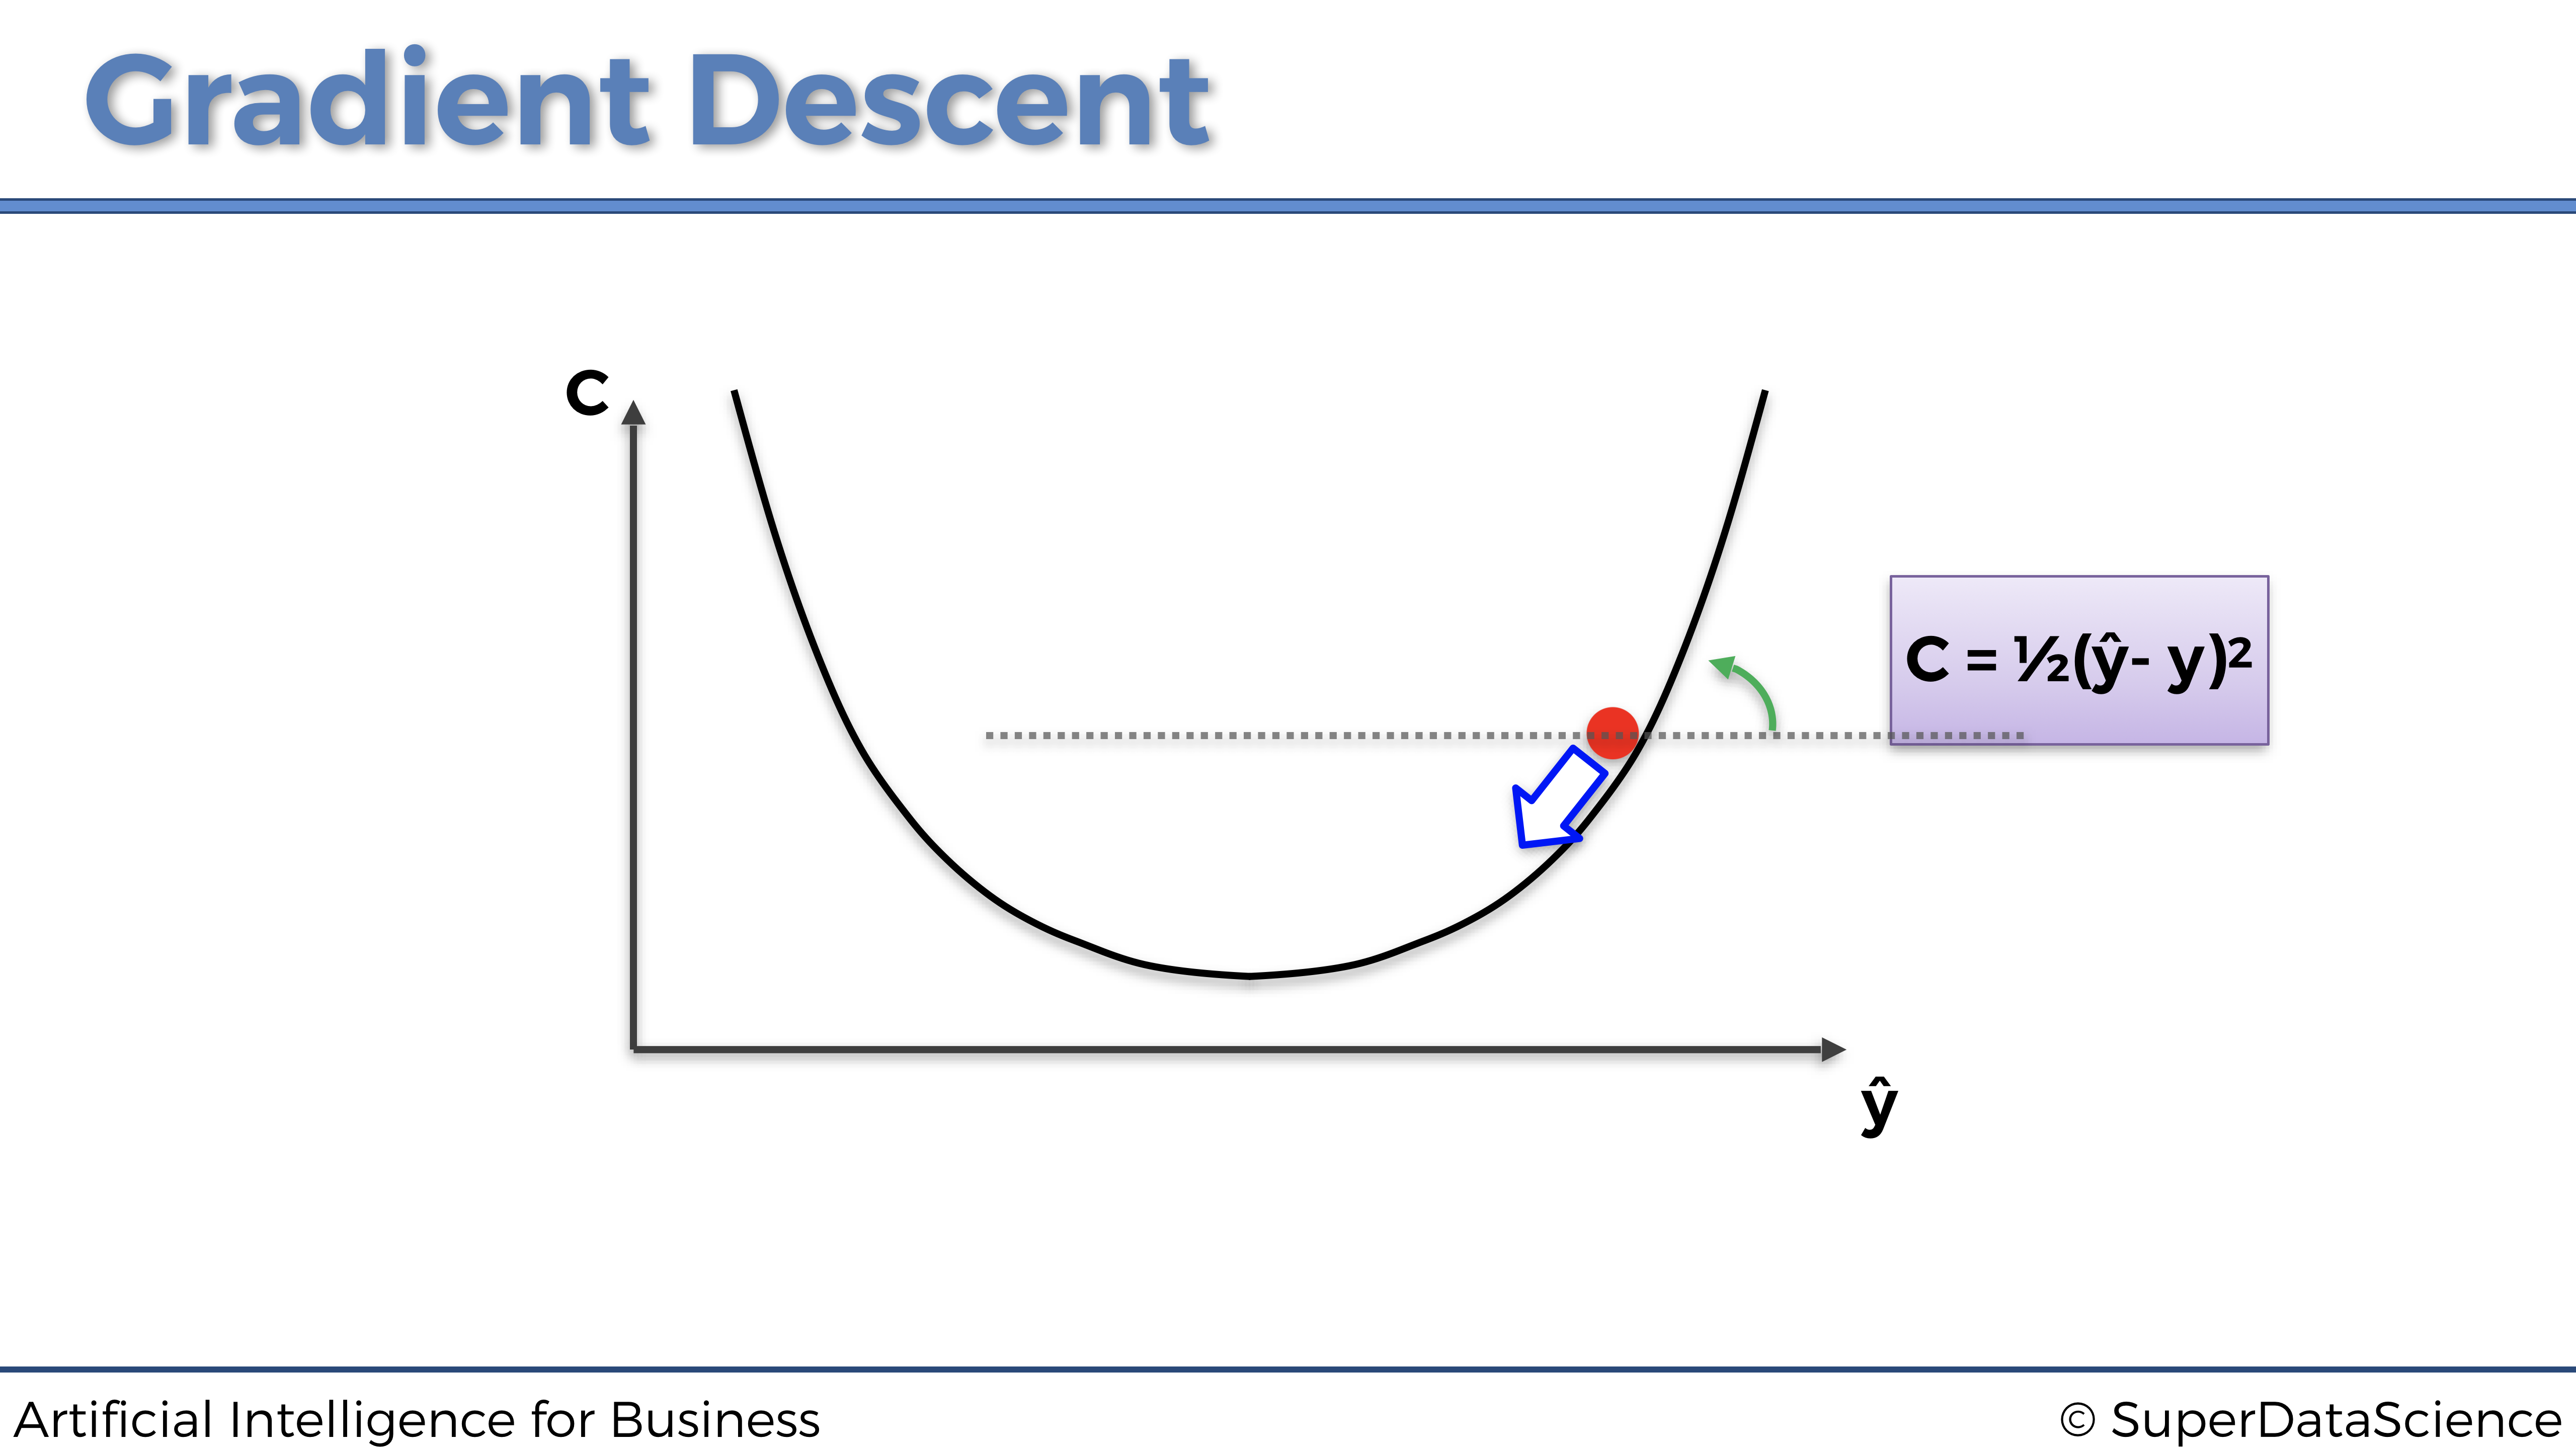
\includegraphics[scale=0.15]{ANN_22.png}
        \end{center}
\end{figure}

Eventually, by repeating the same steps, the ball will end up at the bottom of the bowl:

\begin{figure}[!htbp]
        \begin{center}
            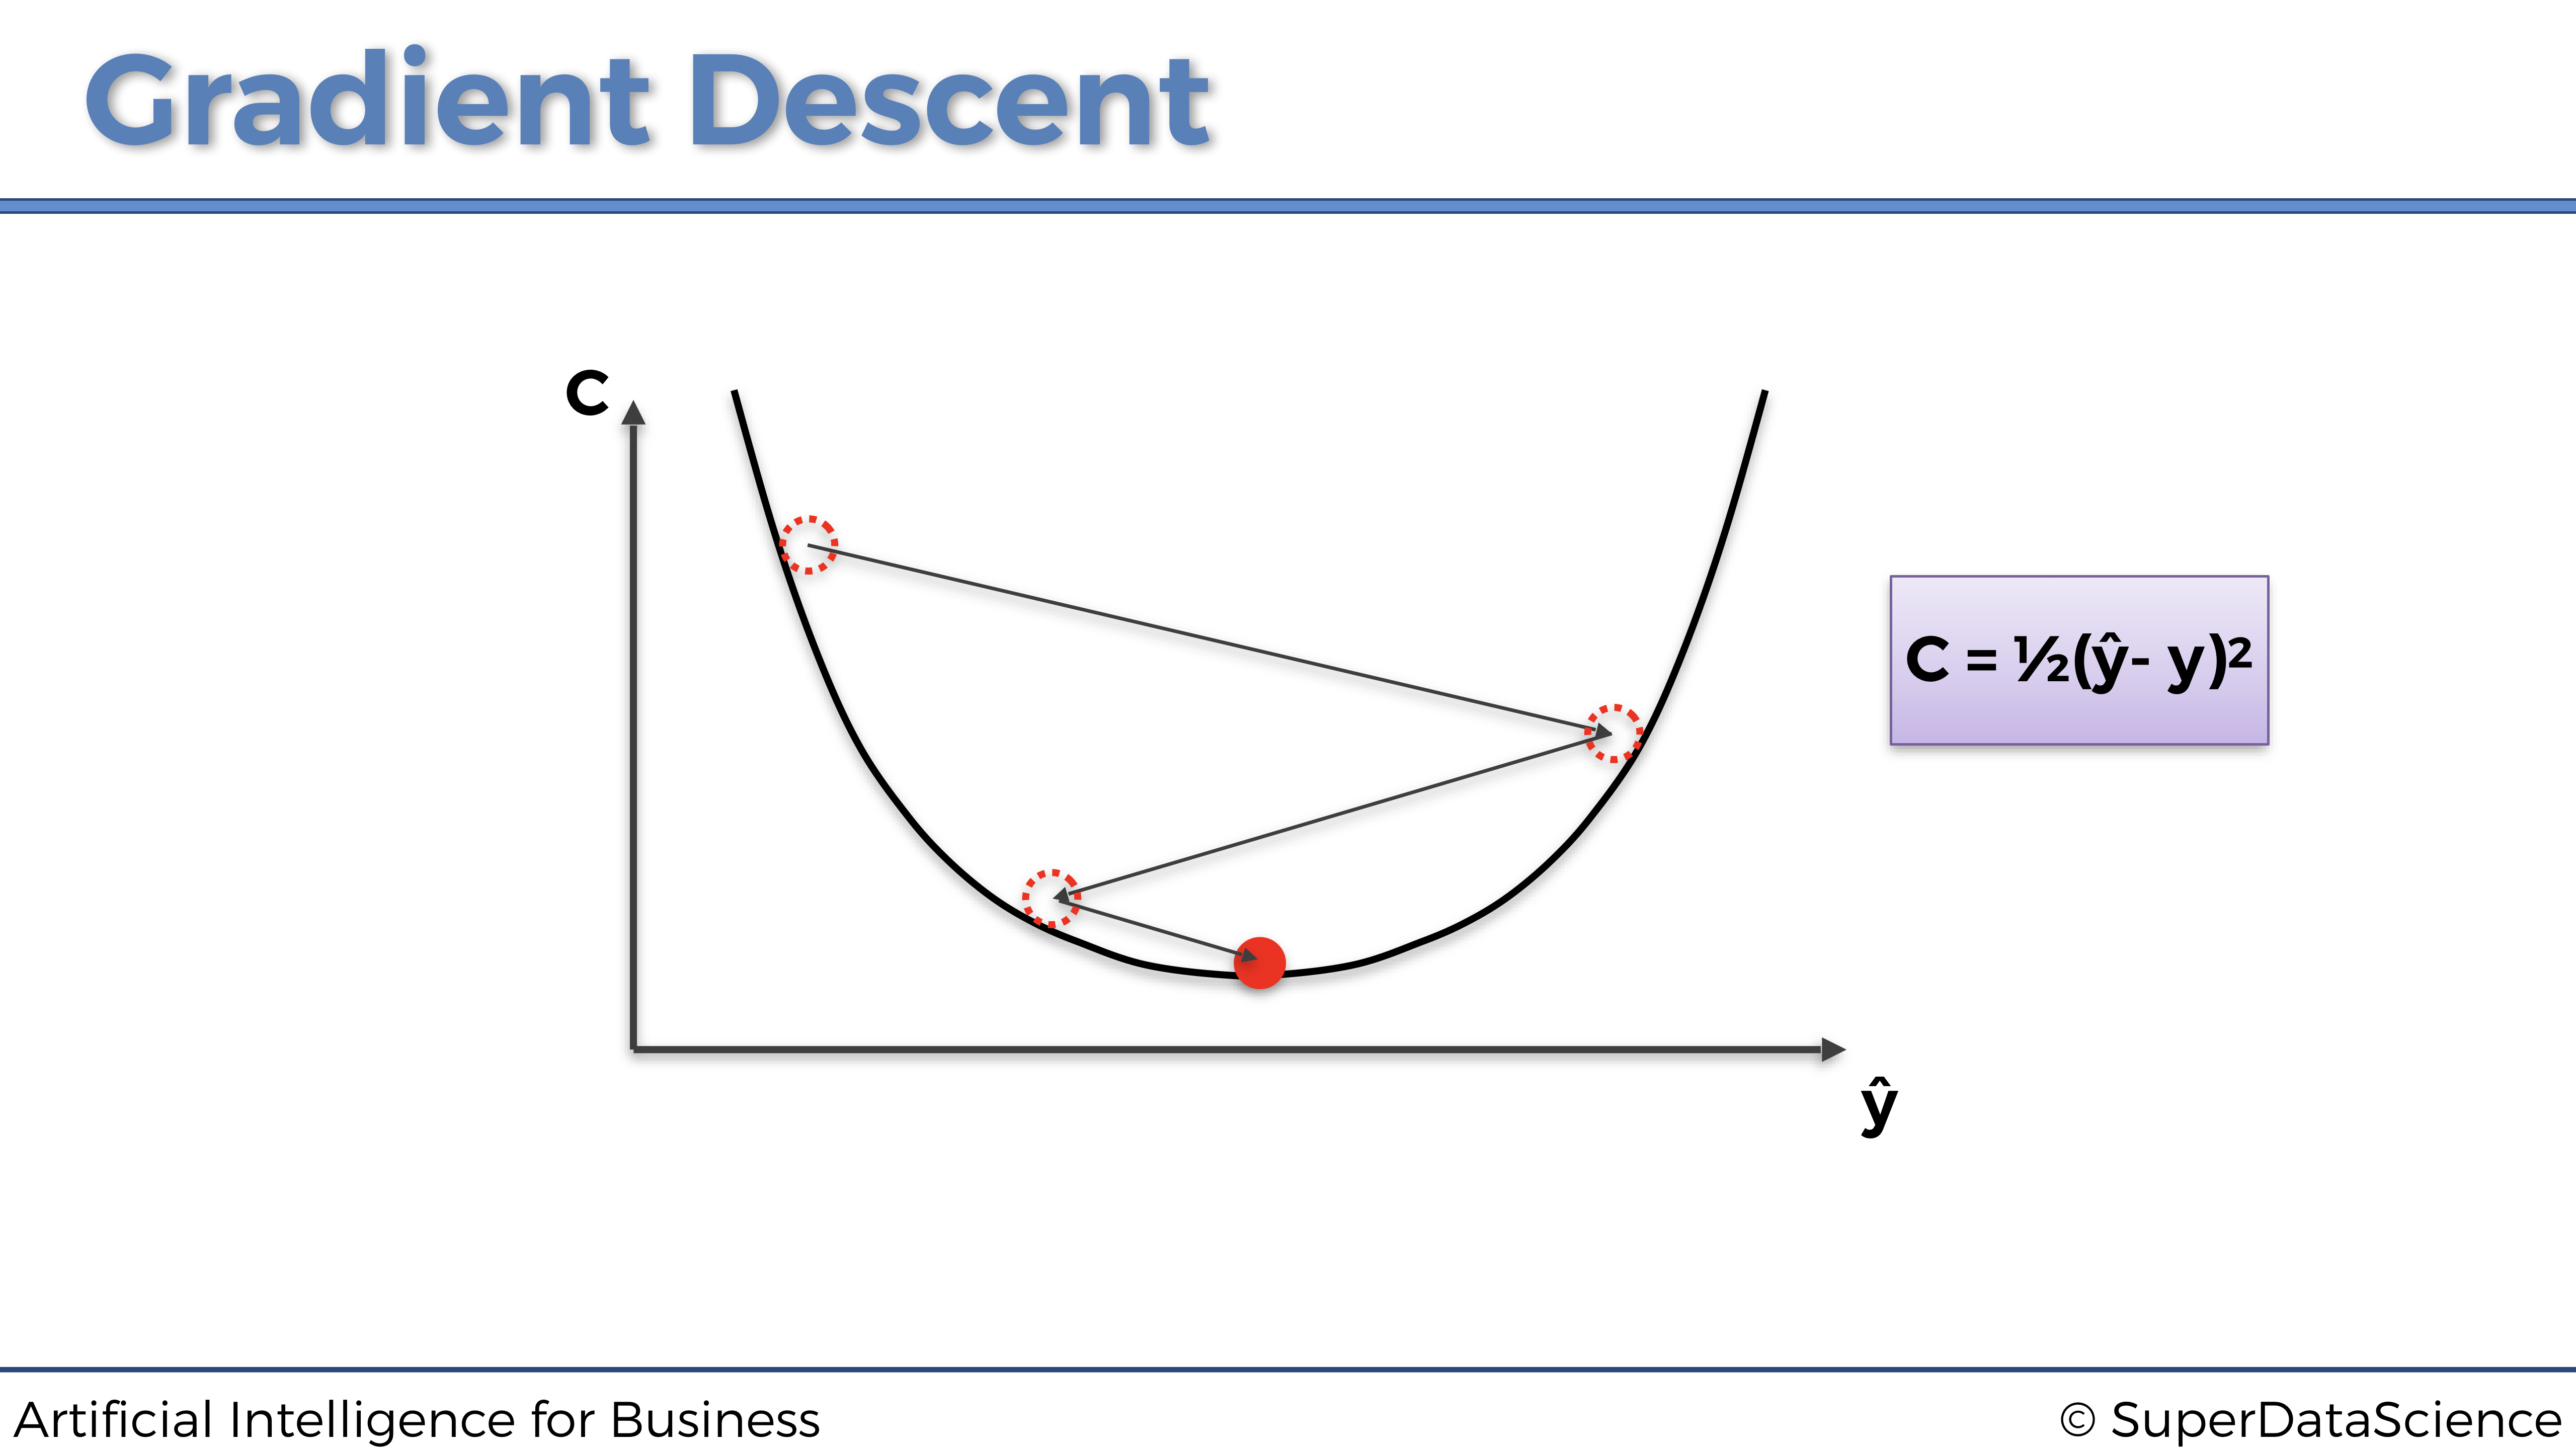
\includegraphics[scale=0.18]{ANN_23.png}
        \end{center}
\end{figure}

And that's it! This is how Gradient Descent operates in one dimension (one parameter). Now you might ask: ``Great, but how does this scale?'' We saw an example of one dimensional optimization, what about two or even 3 dimensions?

Excellent question. Gradient Descent guarantees that this approach scales on as many dimensions as needed, provided the cost function is convex. In fact, if the cost function is convex, Gradient Descent will find the absolute minimum of the cost function. Below is an example in 2 Dimensions:

\begin{figure}[!htbp]
        \begin{center}
            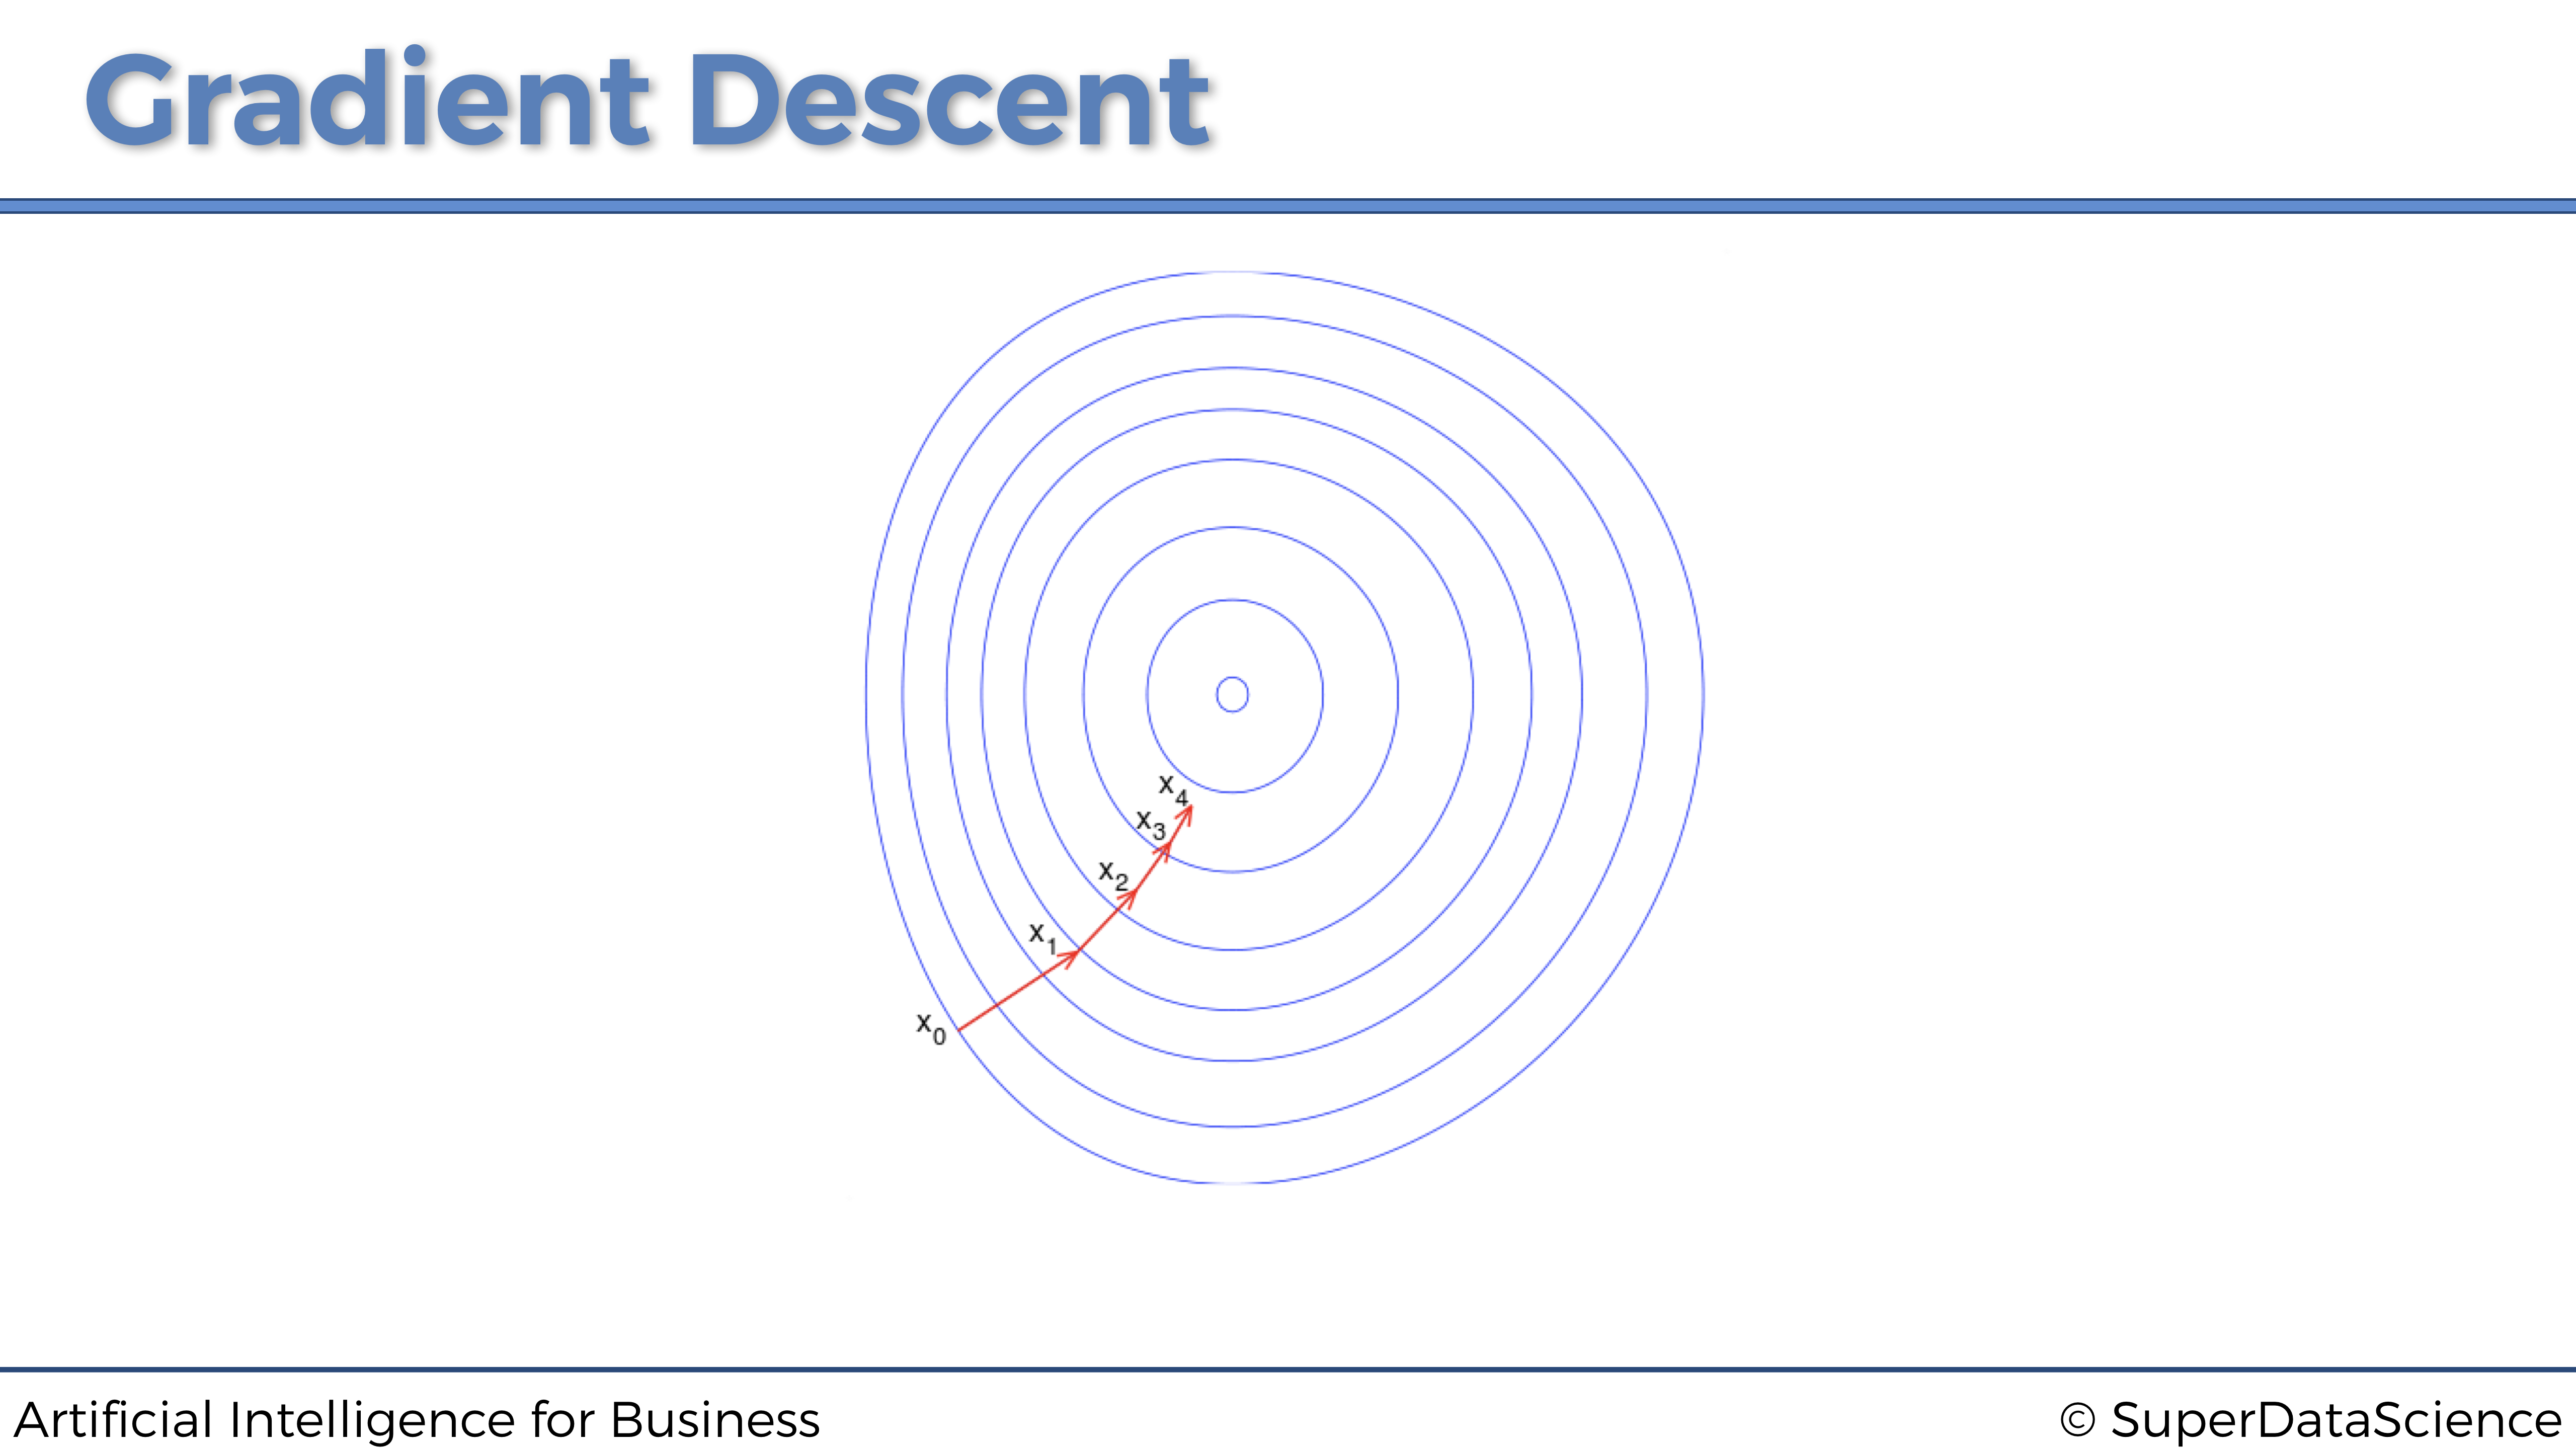
\includegraphics[scale=0.15]{ANN_24.png}
        \end{center}
\end{figure}

However if the cost function is not convex, it will only find a local minimum. Below is an example in 3 Dimensions:

\begin{figure}[!htbp]
        \begin{center}
            \includegraphics[scale=0.15]{ANN_25.png}
        \end{center}
\end{figure}

Now that we understand what Gradient Descent is all about, time to study the most advanced and most effective versions of it:

\begin{enumerate}
    \item Batch Gradient Descent
    \item Mini-Batch Gradient Descent
    \item Stochastic Gradient Descent
\end{enumerate}

\subsection{Batch Gradient Descent}

``Gradient Descent'', ``Batch Gradient Descent'', ``Mini Batch Gradient Descent'', ``Stochastic Gradient Descent''.. There are so many terms and someone who is just starting may found him/her very confused.

The main difference across all of these versions of Gradient Descent is in the way we feed our data to a model, and how often we update our parameters (weights) to move our small red ball. Let's start by explaining Batch Gradient Descent.

Batch Gradient Descent is exactly what we did in Part 2 - Minimizing Costs, where remember we had a batch of inputs feeding the neural network, forward-propagating them to obtain in the end a batch of predictions, which themselves are compared to a batch of targets. The global loss error between the predictions and the targets of the two batches is then computed as the sum of the loss errors between each prediction and its associated target. That global loss is back-propagated into the neural network, where gradient descent or stochastic gradient descent is performed to update all the weights, according to how much they were responsible for that global loss error.

In the next page below is an example of Batch Gradient Descent. The problem to solve is about predicting the score (from 0 to 100 \%) students get at an exam, based on the time spent to study, and the time spent to sleep:

\newpage

\begin{figure}[!htbp]
        \begin{center}
            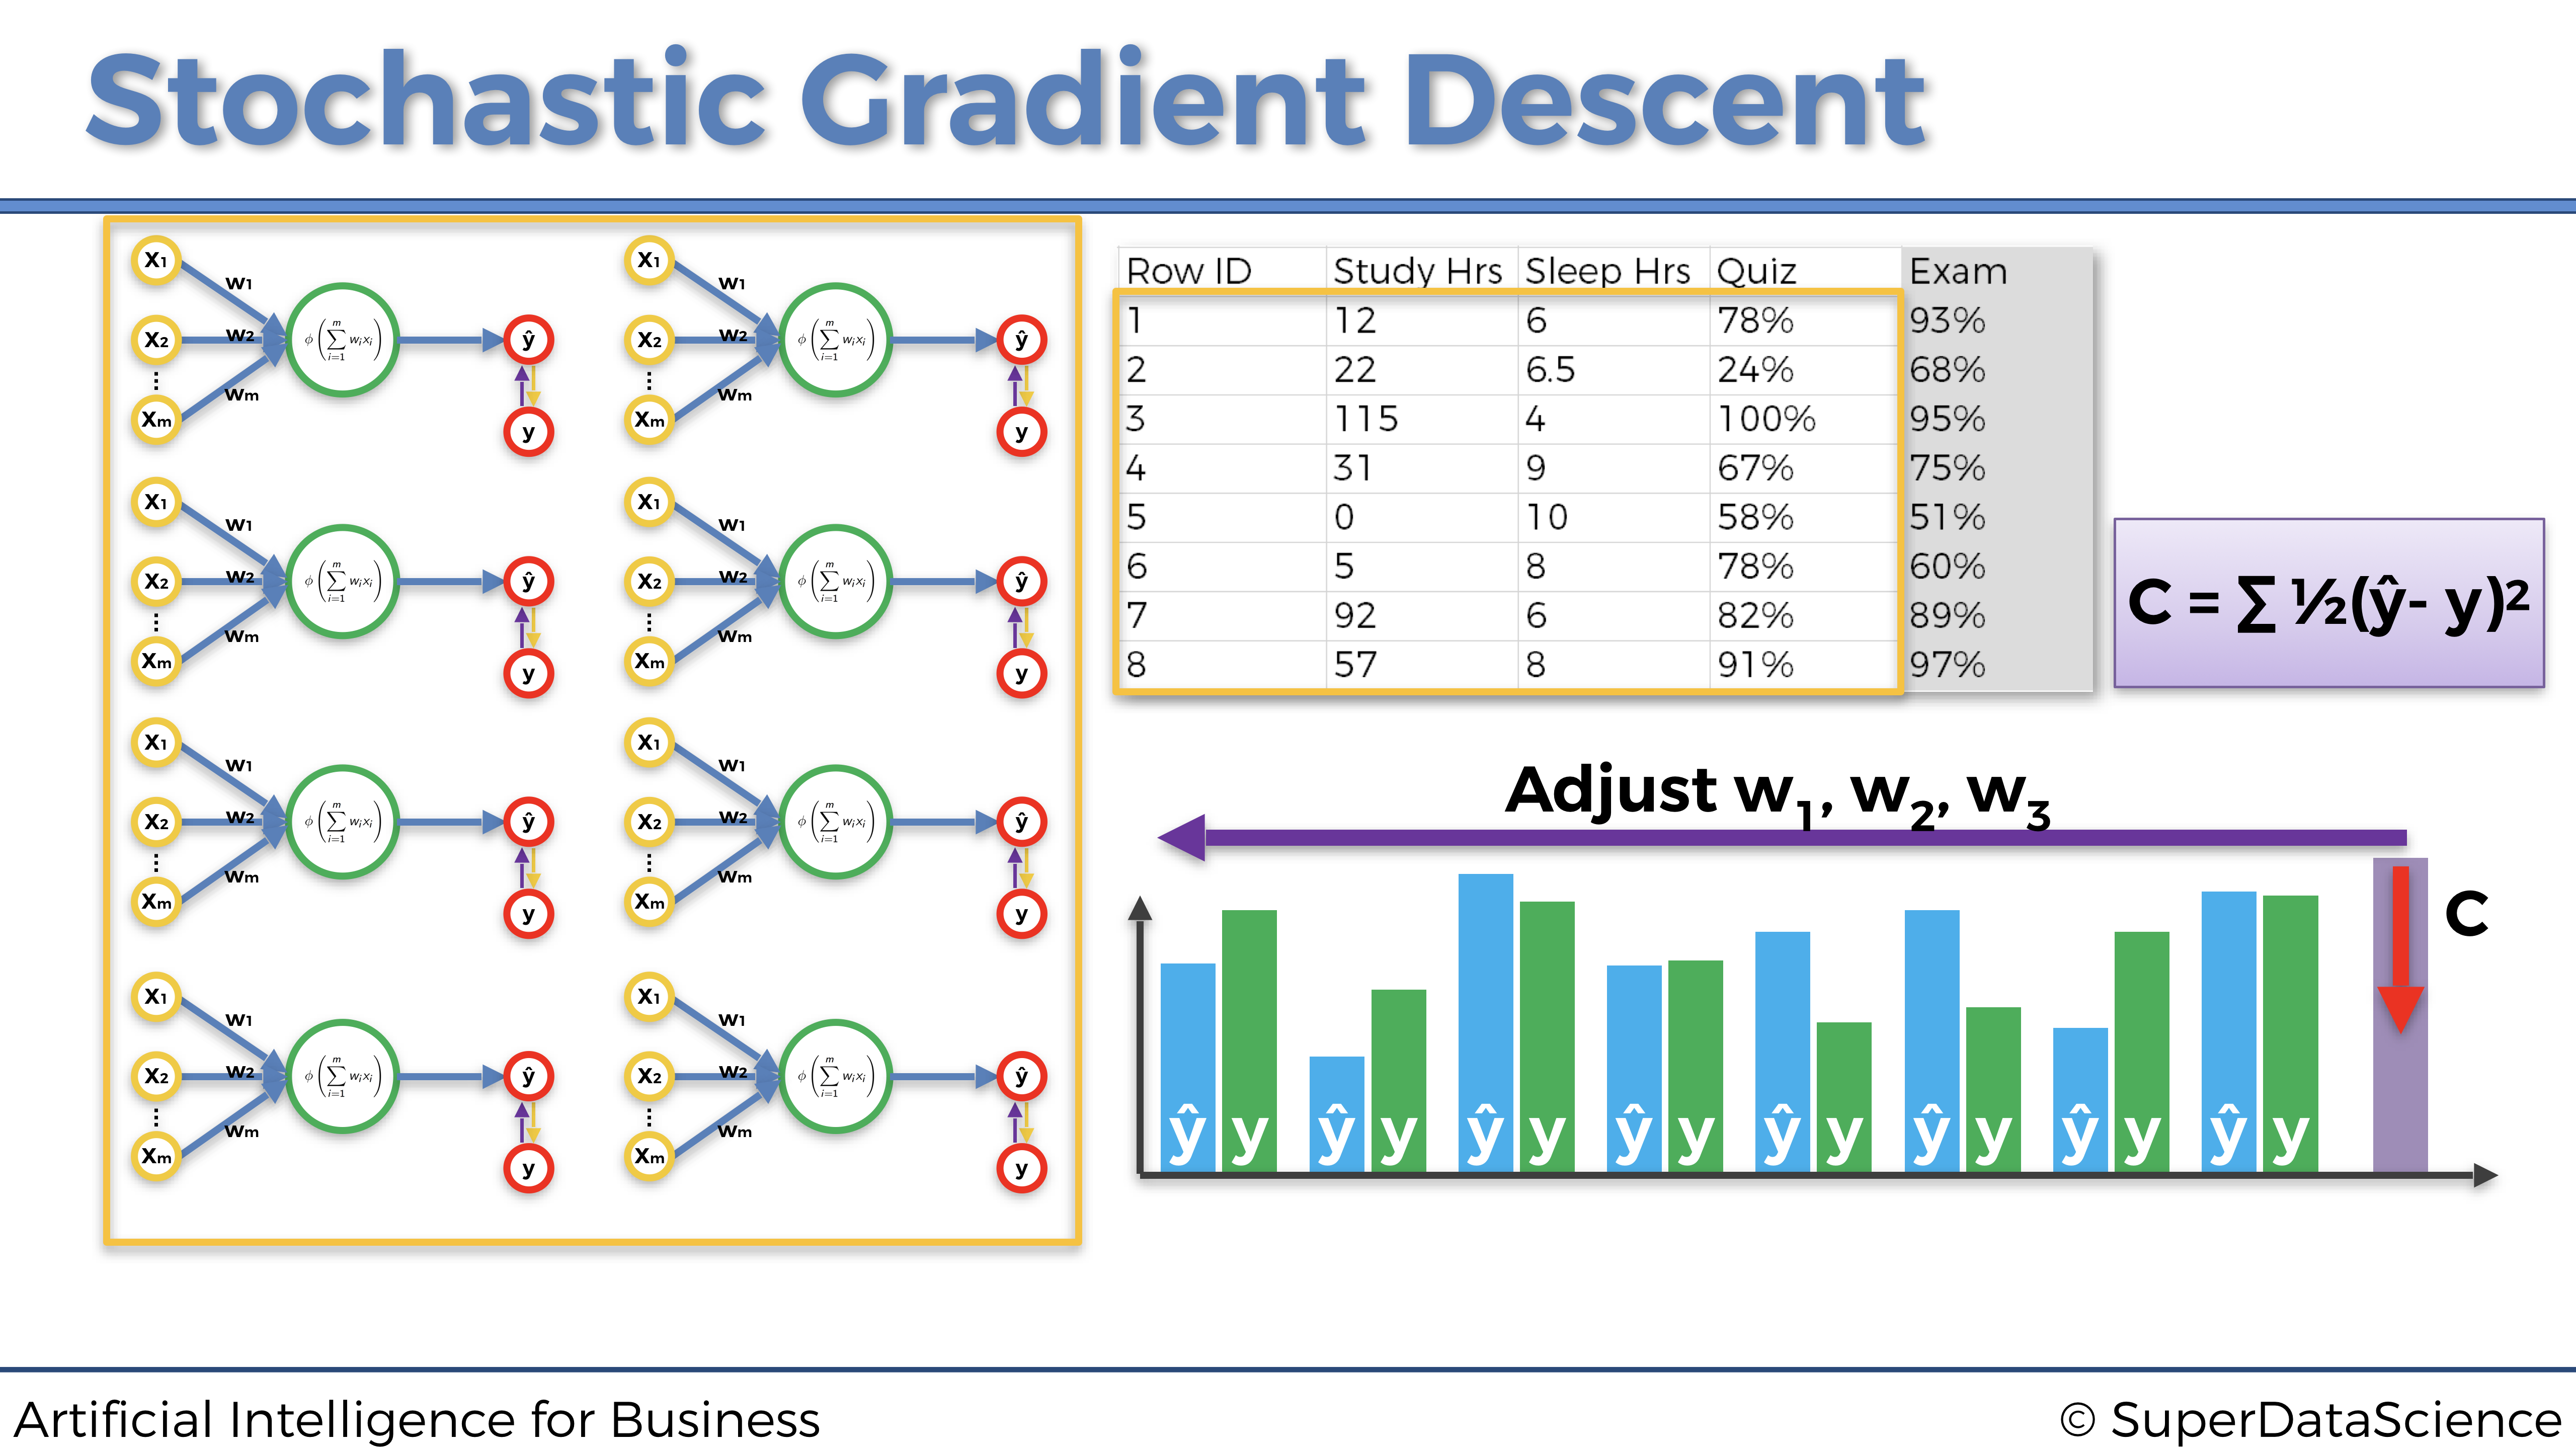
\includegraphics[scale=0.18]{ANN_26.png}
        \end{center}
\end{figure}

An important thing to note on this graphic above is that these are not multiple neural networks, but a single one represented by separate weight updates. And again, as we can notice in this example of Batch Gradient Descent, we feed all of our data to the model at once. This will produce collective updates of the weights and fast optimization of the network. However, there is the bad side of this as well. There is once again the possibility to get stuck at a local minimum, as we can see in the next graphic below:

\begin{figure}[!htbp]
        \begin{center}
            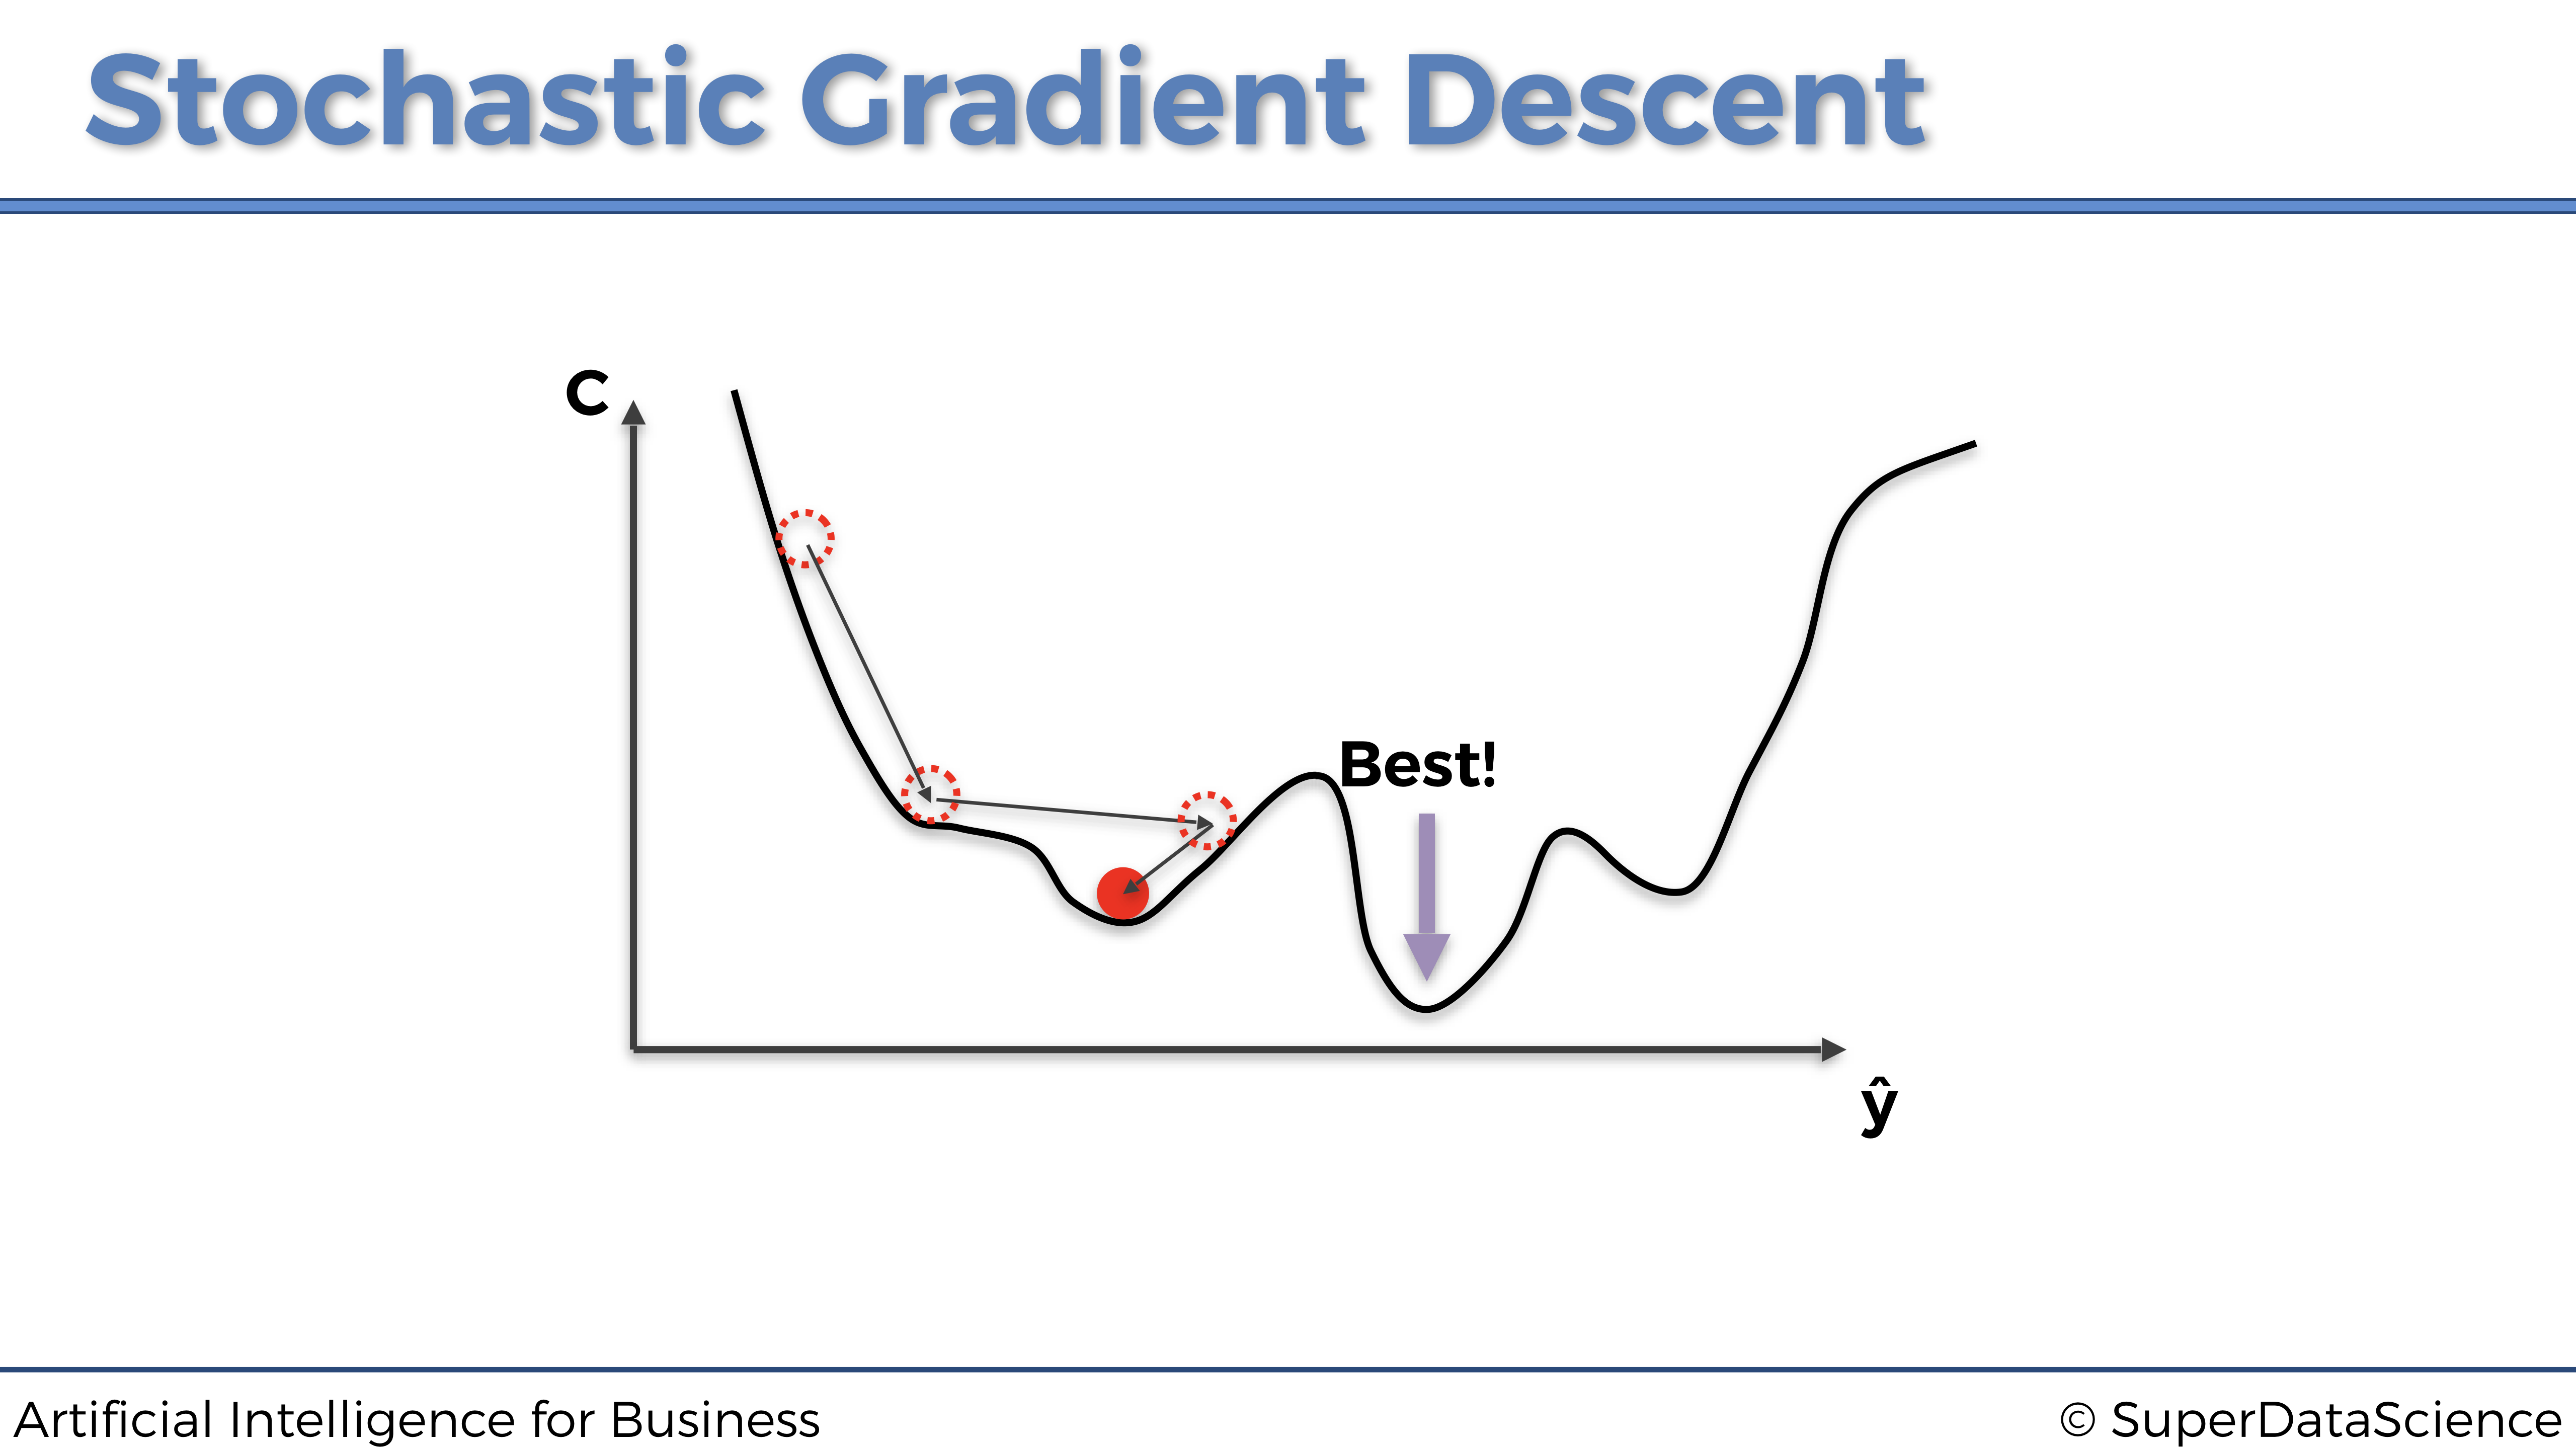
\includegraphics[scale=0.18]{ANN_30.png}
        \end{center}
\end{figure}

\newpage

The reason why this happens was explained a bit earlier: it is because the cost function in the graphic above is not convex. And this type of optimization (simple Gradient Descent) requires the cost function to be convex. If that is not the case we can find ourselves stuck in a local minimum and never find the global minimum having the optimal parameters. On the other hand, below is an example of a convex cost function, the same one as we saw earlier:

\begin{figure}[!htbp]
        \begin{center}
            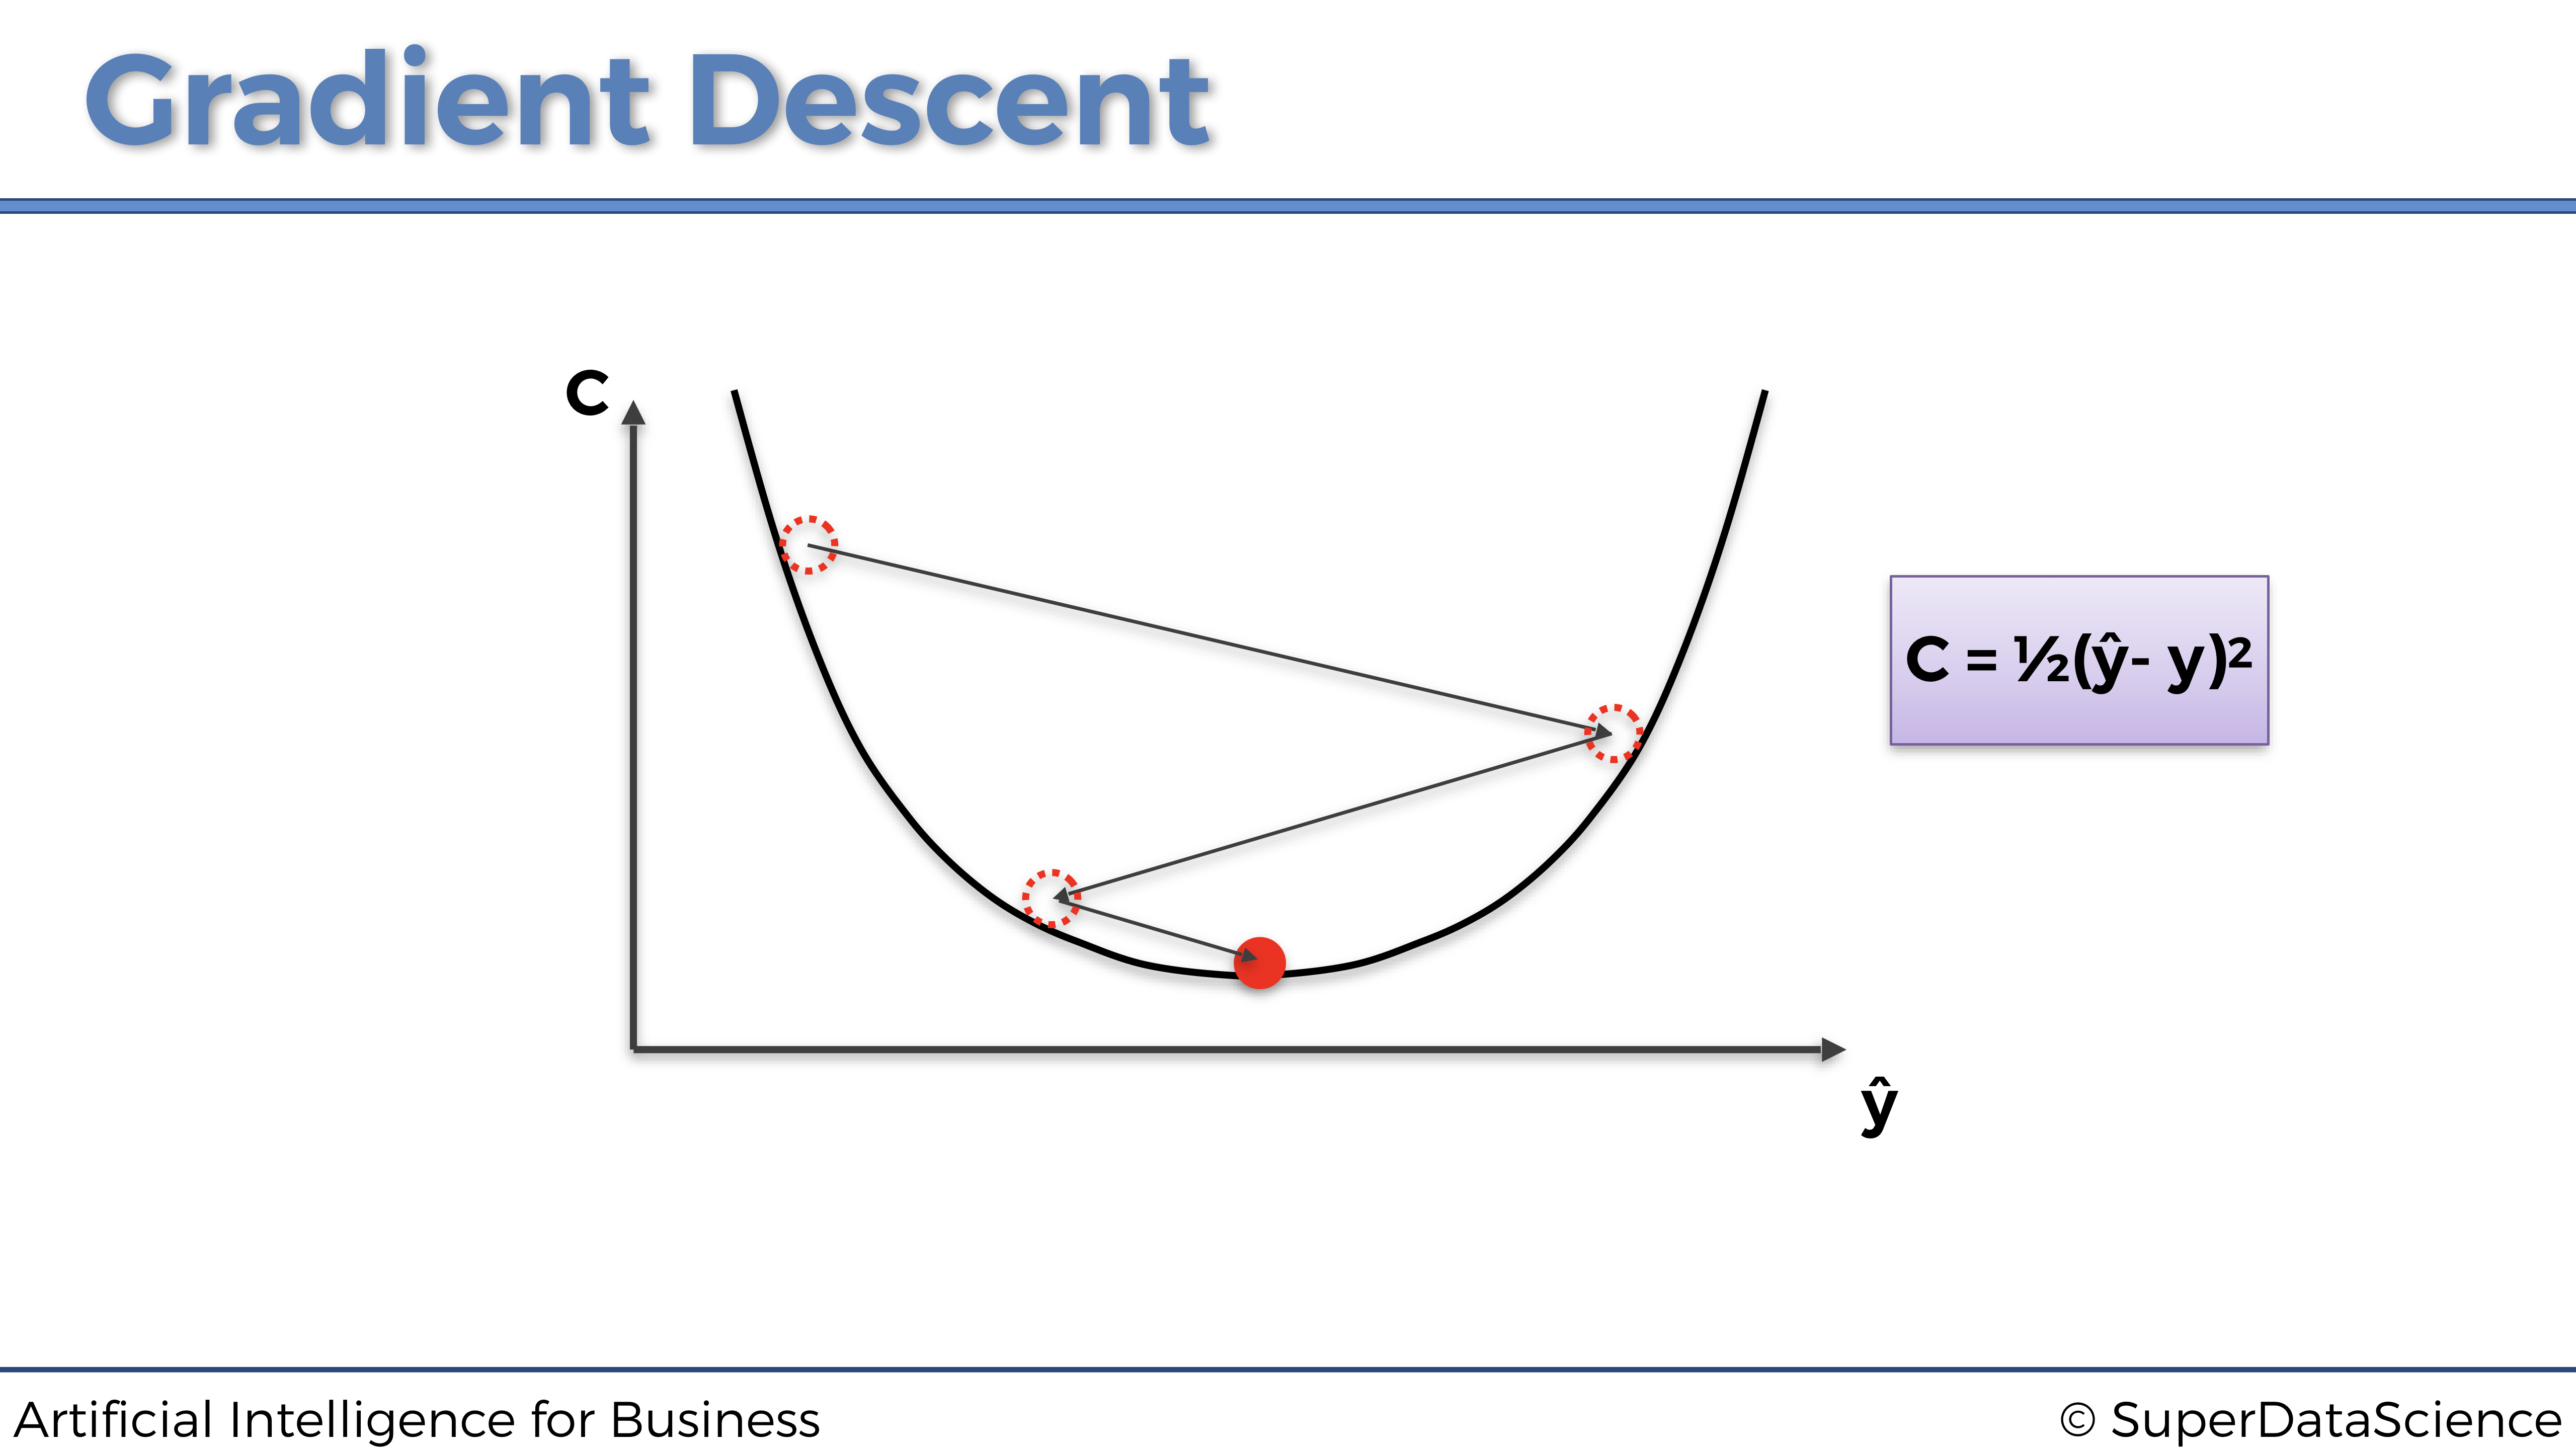
\includegraphics[scale=0.18]{ANN_23.png}
        \end{center}
\end{figure}

In simple terms, a function is convex if it has only one global minimum. And the graph of a convex function has the bowl shape.

However, in most of the problems, including the business problems, the cost function will not be convex (as in this same graphic example in 3D below), thus not allowing simple Gradient Descent to perform well. This is where Stochastic Gradient Descent comes into play.

\begin{figure}[!htbp]
        \begin{center}
            \includegraphics[scale=0.13]{ANN_25.png}
        \end{center}
\end{figure}

\subsection{Stochastic Gradient Descent}

Stochastic Gradient Descent (SGD) comes to save the day. It indeed provides better results overall, preventing the algorithm to get stuck in a local minimum. However, as its name suggests, it is stochastic, or in other words, random. Because of this property, no matter how many times you run the algorithm, the process will always be slightly different. And that, regardless of the initialization.

Stochastic Gradient Descent does not run on the whole dataset at once but instead input by input. Hence, the process goes like this:

\begin{enumerate}
    \item Input a single observation
    \item Get the single prediction
    \item Compute the loss error between the prediction and the target
    \item Back-Propagate the loss error into the neural network
    \item Update the weights with Gradient Descent
    \item Repeat 1. to 5. through the whole dataset
\end{enumerate}

Let's represent the three first iterations on the three first single inputs for this same example given earlier about predicting the scores at an exam:

\textbf{First Input Row of Observation:}

\begin{figure}[!htbp]
        \begin{center}
            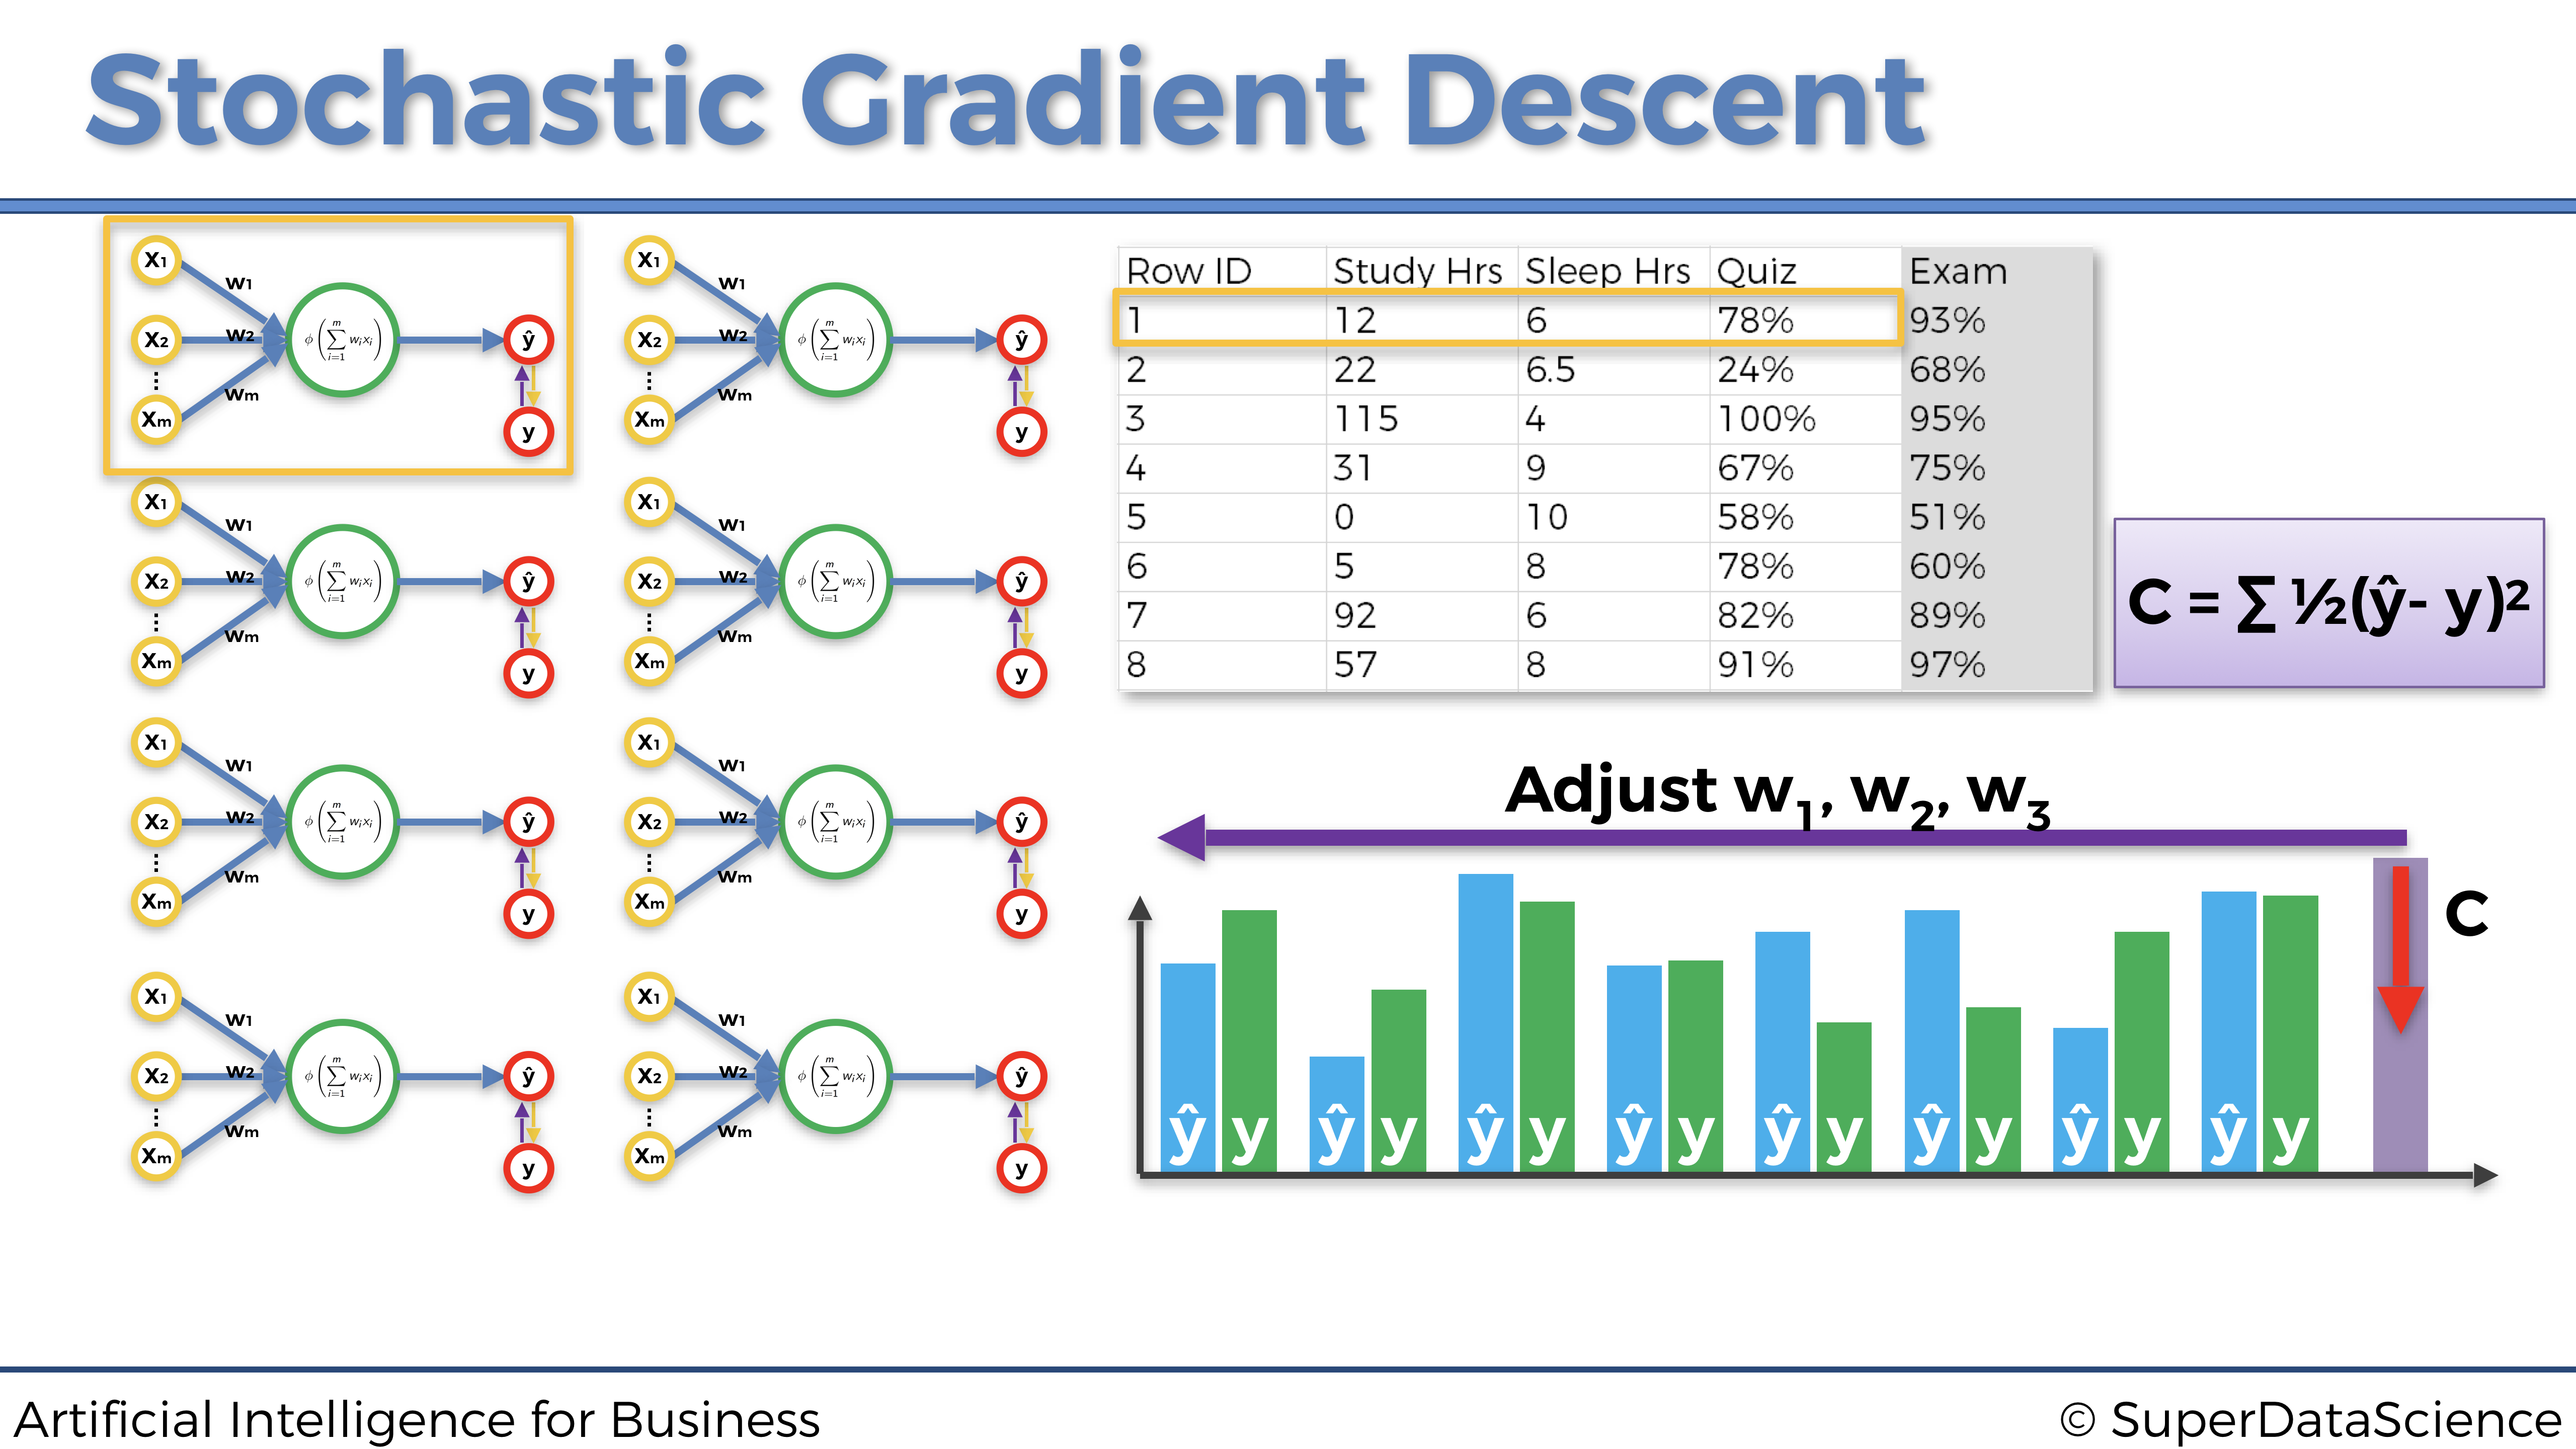
\includegraphics[scale=0.18]{ANN_27.png}
        \end{center}
\end{figure}

\newpage

\textbf{Second Input Row of Observation:}

\begin{figure}[!htbp]
        \begin{center}
            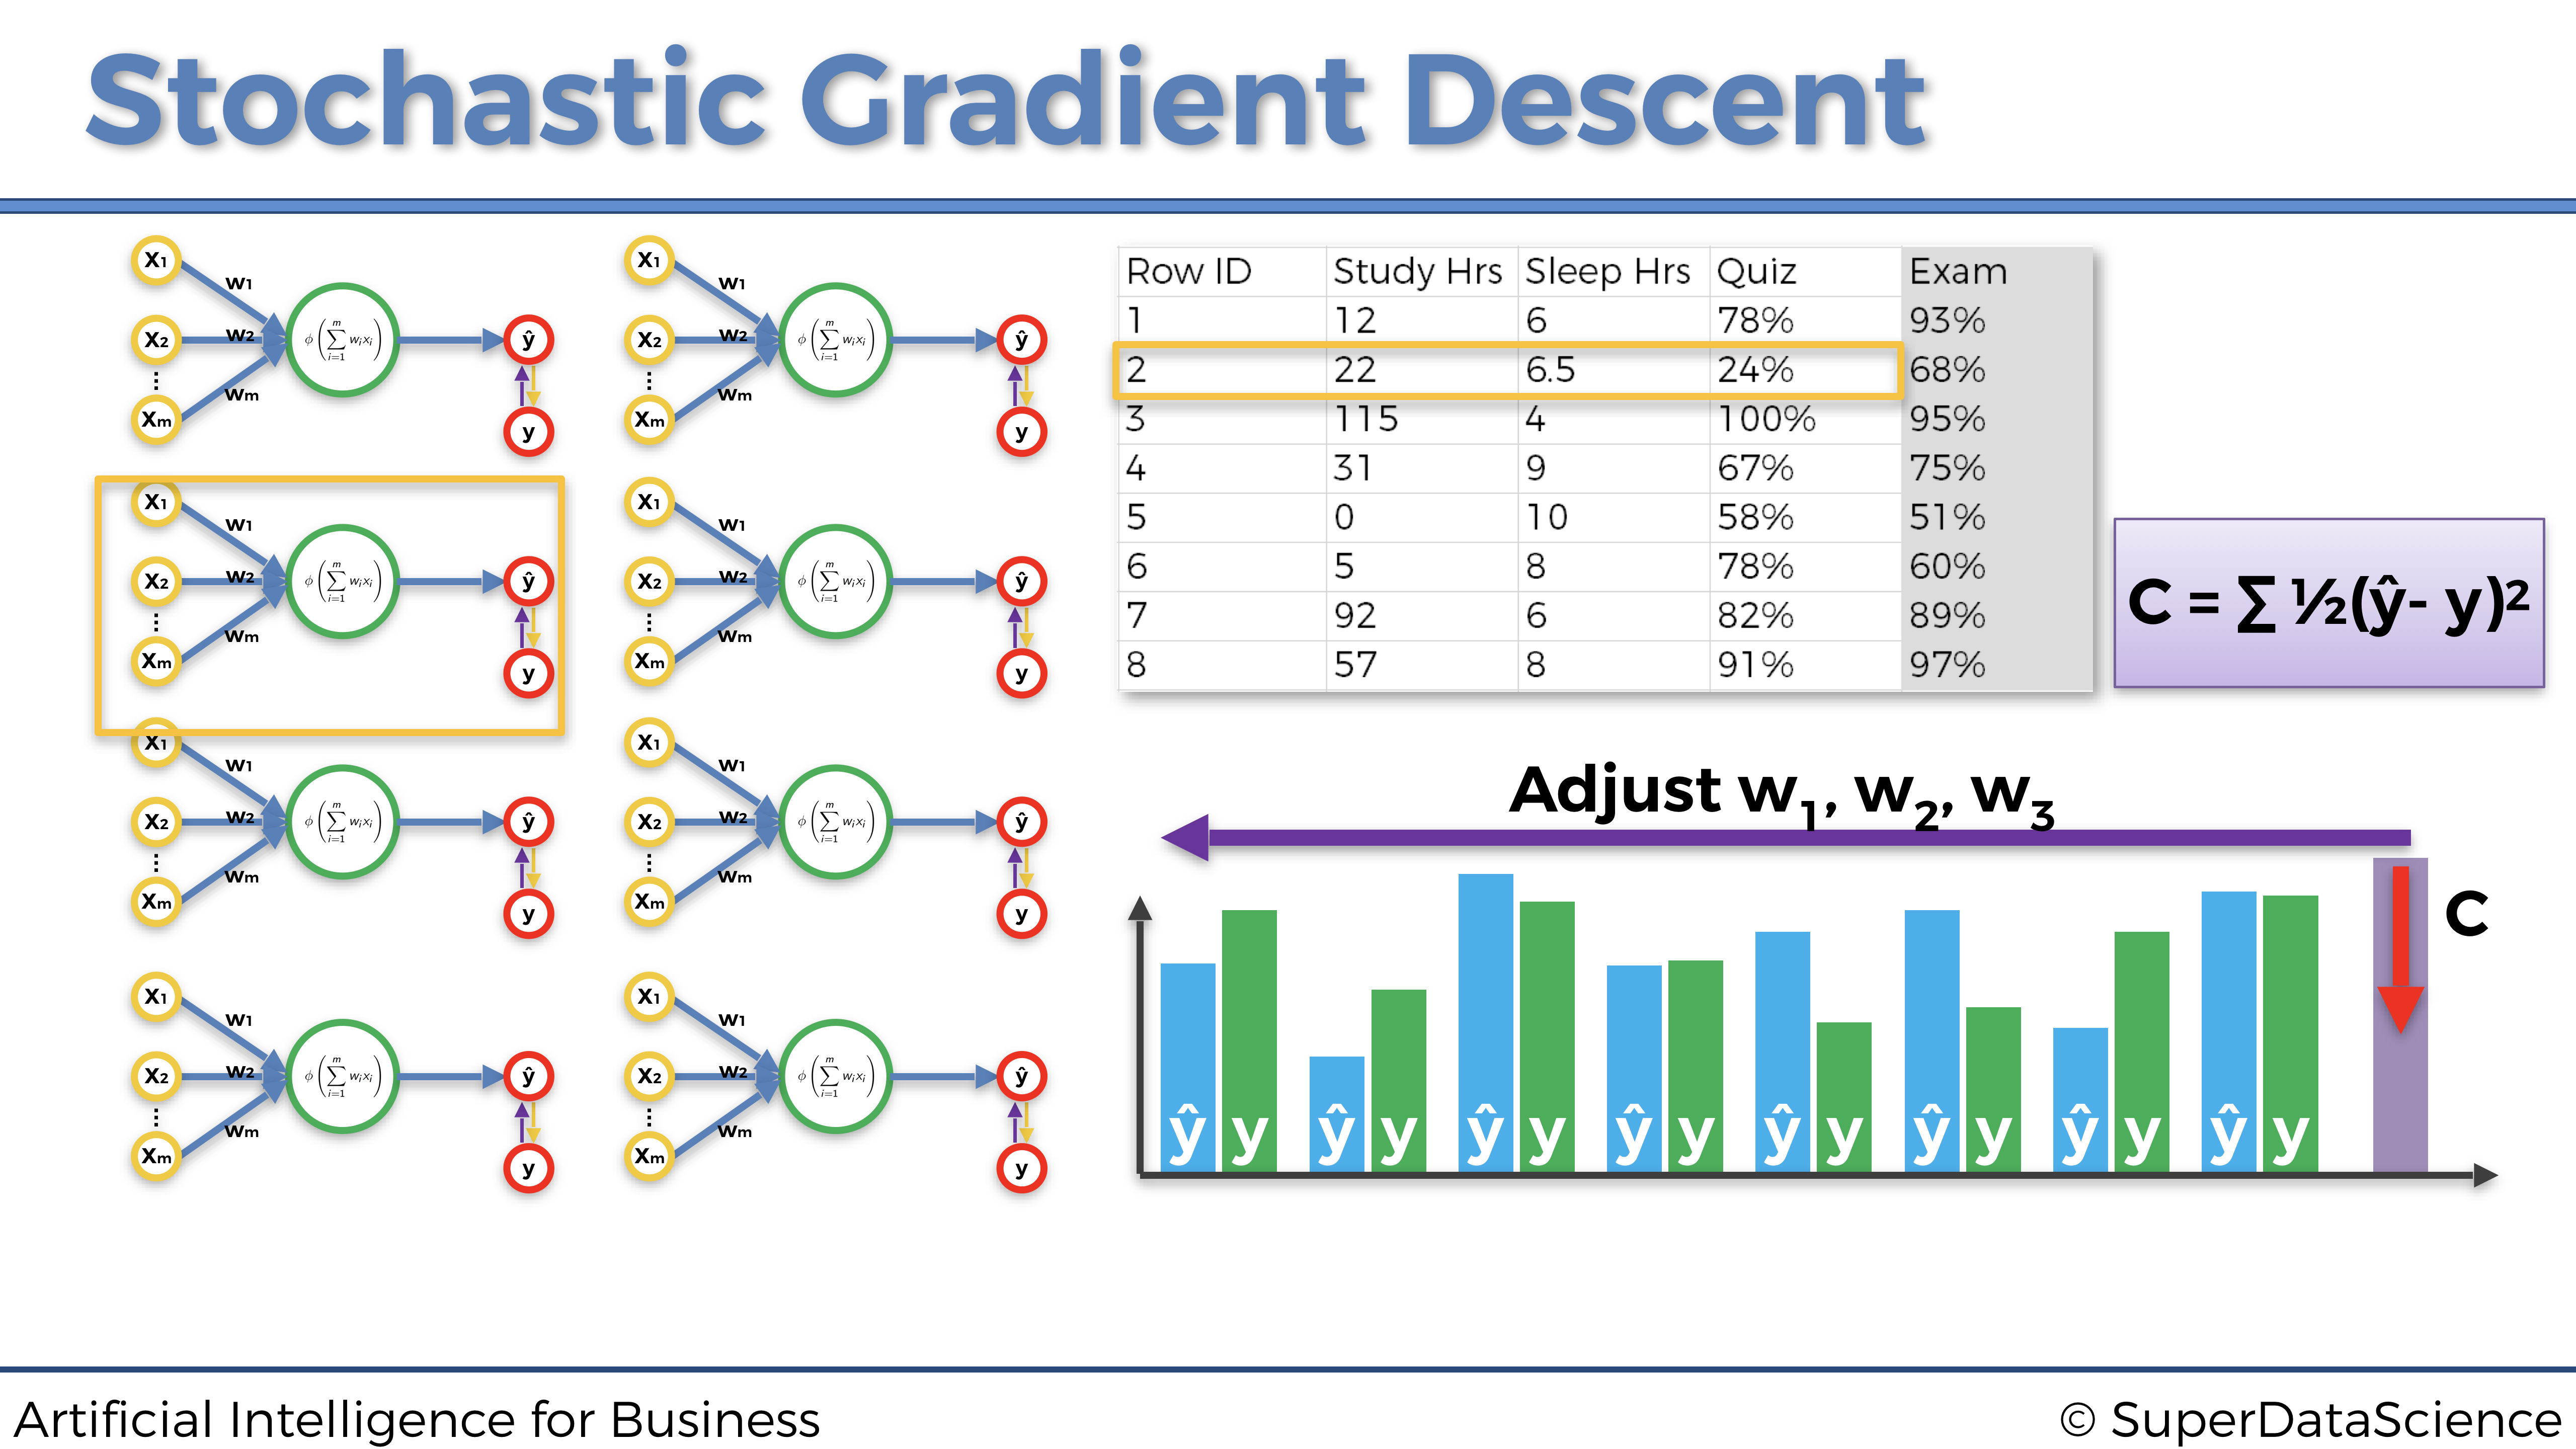
\includegraphics[scale=0.18]{ANN_28.png}
        \end{center}
\end{figure}

\textbf{Third Input Row of Observation:}

\begin{figure}[!htbp]
        \begin{center}
            \includegraphics[scale=0.18]{ANN_29.png}
        \end{center}
\end{figure}

Each of the three graphics above is an example of one weights update ran by Stochastic Gradient Descent. As we can see, each time we only input a single row of observation from our dataset to the neural network, then we update the weights accordingly and proceed to the next input row of observation.

At first glance, Stochastic Gradient Descent seems slower, because we input each row separately. But in reality, it is much faster because of the fact that we don't have to load the whole dataset in the memory, nor to wait for whole dataset to pass through the model updating the weights.

To finish this section, let's recap on the difference between Batch Gradient Descent and Stochastic Gradient Descent, with the following graphic:

\begin{figure}[!htbp]
        \begin{center}
            \includegraphics[scale=0.18]{ANN_31.png}
        \end{center}
\end{figure}

\subsection{Mini-Batch Gradient Descent}

Mini-Batch Gradient Descent is using the best from both worlds to combine Batch Gradient Descent with Stochastic Gradient Descent. This is done by feeding the neural network with batches of data instead of feeding single input rows of observations one by one or the whole dataset at once.

This approach is faster than classical Stochastic Gradient Descent and prevents from getting stuck in the local minimum. This also helps when people don't have enough computing resources to load the whole dataset in the memory, or enough processing power to get full benefit of Stochastic Gradient Descent.

\subsection{Optimizers}

The optimizer is exactly the tool that will update the weights of the Neural Network through Stochastic Gradient Descent. Up to this point we have only mentioned the Adam optimizer (see Part 2 - Minimizing Costs), which is the most common optimizer used for the Deep Learning and Deep Reinforcement Learning models. Nevertheless there are a lot more optimizers which have their own benefits and applications.

Let's go through the most famous and widely used Gradient Descent optimizers.

\newpage

\subsubsection{Momentum Optimizer}

The classical Stochastic Gradient Descent has very big oscillations, which leaves room for improvement. The Momentum optimizer handles these big oscillations by adding fractions of the directions calculated in the previous step to the current step. This amplifies the speed of the current direction update. In the graphic just below we can see and compare the Classical SGD and the Momentum SGD in action:

\begin{figure}[!htbp]
        \begin{center}
            \includegraphics[scale=0.75]{ANN_32.png}
        \end{center}
\end{figure}

The benefits of the Momentum Optimizer are the following:

\begin{itemize}
    \item Faster Convergence
    \item Less Oscillations
\end{itemize}

But the Momentum Optimizer also has drawbacks, which are the following:

\begin{itemize}
    \item Tendency to overshoot the global minimum of the cost function because of the momentum.
    \item Less frequent in Deep Learning libraries, which thus requires the know-how of its implementation.
\end{itemize}

\newpage

\subsubsection{The Nesterov Accelerated Gradient Optimizer}

Yuri Nesterov solved the momentum the overshot minimum problem by reversing the calculation order in the update formula:

\begin{figure}[!htbp]
        \begin{center}
            \includegraphics[scale=0.6]{ANN_33.png}
        \end{center}
\end{figure}

\subsubsection{The AdaGrad (Adaptive Gradients) Optimizer}

The idea of adapting our updates according to the slope of the error function, coming from the Nesterov optimizer, is taken and applied in the AdaGrad Optimizer while optimizing the learning rate as well.

Hence, in the AdaGrad optimizer we have the same principle, not only applied on gradients but also on the learning rate.

Here are the benefits of this optimizer:

\begin{itemize}
    \item The AdaGrad optimizer allows to make big updates for infrequent parameters.
    \item And it allows to make small updates for frequent parameters.
\end{itemize}

And here are the drawbacks:

\begin{itemize}
    \item The Learning Rate is always decreasing, this could lead to very small, if any updates.
    \item Less frequent in Deep Learning libraries, which thus requires the know-how of its implementation.
\end{itemize}

\subsubsection{The AdaDelta Optimizer}

The AdaDelta Optimizer was invented to fix that decreasing learning rate issue of the AdaGrad Optimizer (first drawback). No need to get in further details, we just needed to introduce the AdaDelta optimizer and its particularity in order to understand the strength of the most widely used and most effective optimizer: the Adam Optimizer.

\subsubsection{The Adam (Adaptive Moment Estimation) Optimizer}

The Adam Optimizer is an improvement over the AdaDelta Optimizer. The idea behind it is to store in a memory the momentum changes, as we calculate the learning rate for each parameter separately.

Now remember the benefits of the Adam Optimizer, which are to be considered whenever building a Neural Network.

\begin{itemize}
    \item It is one of the most powerful optimizers.
    \item It is always pre-implemented in the Deep Learning libraries (Keras, TensorFlow, PyTorch). You will not miss it.
\end{itemize}

Of course, this is the one we use when building the Artificial Brain of our AI in Part 2 - Minimizing the Costs. Let's again provide the code that builds this artificial brain and notice, at the last line of code, the simplicity of selecting the Adam Optimizer:

\begin{lstlisting}
# Artificial Intelligence for Business - Case Study 2
# Building the Brain

# Importing the libraries
from keras.layers import Input, Dense
from keras.models import Model
from keras.optimizers import Adam

# BUILDING THE BRAIN

class Brain(object):
    
    # BUILDING A FULLY CONNECTED NEURAL NETWORK DIRECTLY INSIDE THE INIT METHOD
    
    def __init__(self, learning_rate = 0.001, number_actions = 5):
        self.learning_rate = learning_rate
        
        # BUILDIND THE INPUT LAYER COMPOSED OF THE INPUT STATE
        states = Input(shape = (3,))
        
        # BUILDING THE FULLY CONNECTED HIDDEN LAYERS
        x = Dense(units = 64, activation = 'sigmoid')(states)
        y = Dense(units = 32, activation = 'sigmoid')(x)
        
        # BUILDING THE OUTPUT LAYER, FULLY CONNECTED TO THE LAST HIDDEN LAYER
        q_values = Dense(units = number_actions, activation = 'softmax')(y)
        
        # ASSEMBLING THE FULL ARCHITECTURE INSIDE A MODEL OBJECT
        self.model = Model(inputs = states, outputs = q_values)
        
        # COMPILING THE MODEL WITH AN MSE LOSS FUNCTION AND THE ADAM OPTIMIZER
        self.model.compile(loss = 'mse', optimizer = Adam(lr = learning_rate))
\end{lstlisting}

\newpage

\hypertarget{annex-2-three-extra-ai-models}{%
\chapter{Annex 2: Three Extra AI Models}\label{annex-2-three-extra-ai-models}}

As a Bonus, in this section we provide three extra AI models, closer to the State of the Art. However, these AI models are not necessarily adapted to solve business problems, but more to solve specific tasks like playing games or training a virtual robot to walk. We are going to study three powerful models, including two in the Deep Reinforcement Learning branch of AI, and one in the Policy Gradient branch:

\begin{enumerate}
    \item Deep Convolutional Q-Learning (Deep RL)
    \item A3C (Deep RL)
    \item Augmented Random Search (Policy Gradient)
\end{enumerate}

\subsection{Deep Convolutional Q-Learning}

In the previous section, our inputs were vectors encoded values defining the states of the environment. But since an encoded vector doesn't preserve the spatial structure of an image, this is not the best form to describe a state. The spatial structure is indeed important because it gives us more information to predict the next state, and predicting the next state is of course essential for our AI to know what is the right next move. Therefore we need to preserve the spatial structure and to do that, our inputs must be 3D images (2D for the array of pixels plus one additional dimension for the colors). In that case, the inputs are simply the images of the screen itself, exactly like what a human sees when playing the game. Following this analogy, the AI acts like a human: it observes the input images of the screen when playing the game, the input images go into a convolutional neural network (the brain for a human) which will detect the state in each image. However, this convolutional neural network doesn't contain pooling layers, because they would loose the location of the objects inside the image, and of course the AI need to keep track of the objects. Therefore we only keep the convolutional layers, and then by flattening them into a 1-dimensional vector, we get the input of our previous Deep Q-Learning network. Then the same process is being ran.

Therefore in summary, Deep Convolutional Q-Learning is the same as Deep Q-Learning, with the only difference that the inputs are now images, and a Convolutional Neural Network is added at the beginning of the fully-connected Deep Q-Learning network to detect the states (or simply the objects) of the images.

\begin{figure}[!htbp]
        \begin{center}
            \includegraphics[scale=0.3]{DCQL}
            \caption{Deep Convolutional Q-Learning}
        \end{center}
\end{figure}

\newpage

\subsection{Asynchronous Actor-Critic Agents (A3C)}

\subsubsection{A3C Intuition}

So far, the action played at each time has been the output of one neural network, as if only one agent was deciding the strategy to play the game. This will no longer be the case with A3C. This time, we are going to have several agents, each one interacting with its own copy of the environment. Let's say there are \(n\) agents \(A_1\), \(A_2\),\ldots{}, \(A_n\).

Each agent is sharing two networks: the actor and the critic. The critic evaluates the present states, while the actor evaluates the possible values in the present state. The actor is used to make decisions. At each epoch time of training for on agent, it takes the last version of the shared networks and uses the actor during n steps in order to make a decision. Over the n steps, it collects all the observed new states, the values of these new states, the rewards, etc\ldots{} After the n steps, the agent uses the collected observations in order to update the shared models. The times of epoch, and therefore the times of updates of the shared network by the agent are not synchronous, hence the name.

That way, if an unlucky agent starts to be stuck into a suboptimal but attractive policy, it will reach out that state -- because other agents also updated the shared policy before the agent got stuck -- and will continue effective exploration.

In order to explain the update rules of the actor and the critic, let us see the networks as functions that depend on vectors of parameters \(\theta\) (for the actor) and \(\theta_v\) (for the critic).

\subsubsection{The whole A3C Process}

The official A3C algorithm is the one of the Google DeepMind paper, ``Asynchronous Methods for Deep Reinforcement Learning'' (\url{https://arxiv.org/pdf/1602.01783.pdf}). In this paper you will find it in the following S3 algorithm:

\begin{figure}[!htbp]
        \begin{center}
            \includegraphics[scale=0.4]{S3}
            \caption{A3C algorithm (https://arxiv.org/pdf/1602.01783.pdf)}
        \end{center}
\end{figure}

\begin{figure}[!htbp]
        \begin{center}
            \includegraphics[scale=0.4]{A3C}
            \caption{A3C}
        \end{center}
\end{figure}

In this figure above we can clearly see the three As of the A3C:

\begin{itemize}

\item[$\bullet$] \textbf{Asynchronous}: There are several agents, each one having their own copy of the environment, and all asynchronised (playing the game at different times).

\item[$\bullet$] \textbf{Advantage}: The advantage is the difference between the prediction of the actor, $Q(s,a)$, and the prediction of the critic, $V(s)$:

\begin{equation*}
A = Q(s,a) - V(s)
\end{equation*}

\item[$\bullet$] \textbf{Actor-Critic}: Of course we can see the actor and the critic, that therefore generate two different losses: the policy loss and the value loss. The policy loss is the loss related to the predictions of the actor. The value loss is the loss related to the predictions of the critic. Over many epochs of the training, these two losses will be back-propagated into the Neural Network, then reduced with an optimizer through stochastic gradient descent.

\end{itemize}

\newpage

\subsection{Augmented Random Search}

\subsubsection{Problem to solve}

We want to build and train an AI that walks or runs across a field. The field is a flat ground that looks like this:

\begin{figure}[!htbp]
        \begin{center}
            \includegraphics[scale=0.15]{Half_Cheetah.png}
        \end{center}
\end{figure}

On this same field you can see a Half-Cheetah. This will be one of the agents we will train to walk on this field. Both the field and the agent form what we call an environment, which belongs to PyBullet, the official Python Interface for the Bullet Physics SDK specialized for Robotics Simulation and Reinforcement Learning, built and developed by Erwin Coumans. For more info click \href{https://docs.google.com/document/d/10sXEhzFRSnvFcl3XxNGhnD4N2SedqwdAvK3dsihxVUA/edit}{here}. You can also check the GitHub page on this \href{https://github.com/bulletphysics/bullet3}{link}.

\subsubsection{AI Solution}

The solution to our problem is a very recent AI model called \textbf{ARS}, or \textbf{Augmented Random Search}. The related research paper was released by Horia Mania, Aurelia Guy and Benjamin Recht on March 20, 2018. You can find the full research paper \href{https://arxiv.org/pdf/1803.07055.pdf}{here}.

ARS is based on a specific branch of Artificial Intelligence called Evolution Strategies. The difference is that ES uses parallelized deep neural networks of several layers, while ARS uses a simple linear policy, which is a Perceptron (a shallow neural network of one layer composed of several neurones). ARS is also slightly similar to \textbf{PPO} - \textbf{Proximal Policy Optimization}, in the sense that ARS aims to optimize a policy (a function of the states returning the actions to play) that performs the best actions allowing the AI to walk. However the technique is different. If you are curious about \textbf{PPO}, you can check out the research paper \href{https://arxiv.org/pdf/1707.06347.pdf}{here}.

Now let's deep dive into the ARS.

The whole picture is pretty simple. We have a policy, that takes as inputs the states of the environment, and returns as outputs the actions to play in order to walk and run across a field. Now before we start explaining the algorithm, let's describe in more details the inputs, the outputs and the policy.

\textbf{The inputs.}

The input is a vector encoding the states of the environment. What does it mean? First let's explain what exactly is a state of the environment. A state is the exact situation happening at a specific time \(t\), e.g:

\begin{figure}[!htbp]
        \begin{center}
            \includegraphics[scale=0.5]{Cheetah_in_the_air.png}
        \end{center}
\end{figure}

We can see the cheetah in the air, back legs up, front legs bent, about to land on the ground. All this is encoded into a vector. How? By simply gathering enough values that can describe what is happening here. So the encoded vector will contain the coordinates of the angular points of the cheetah, as well as the angles of rotation around the rotors, and more values like the velocity. Therefore at each time \(t\), a vector of same format is encoding what is happening exactly in the environment. This encoded vector is what we call the input state of the environment, and will be the input of our policy that we will try to optimize.

\textbf{The outputs.}

The output, returned by our policy, is a group of actions played by the agent. More precisely, these actions are the different muscles impulsions of the agent. For example, one of the actions will be the intensity of the muscle pushing the back leg at the level of the foot. What is important to understand here is more the fact that the policy is returning a \underline{group of actions} as opposed to a single action. Indeed a common practice in Reinforcement Learning is to return one discreet action at each time \(t\). Here, not only we return a group of actions, but each of these actions is continuous. Indeed, in order for an agent to walk on a field, it has to move all the parts of its body at each time \(t\), as opposed to only one leg for example. And the actions are continuous because the impulsions of the muscles are measured by continuous metrics. Hence, the output is also a vector of several continuous values, just like the input state.

\textbf{The policy.}

Between the inputs and the outputs we have a policy, which is nothing else than a function, taking as inputs the input states, and returning as outputs the actions to play, i.e.~the muscle impulsions. This policy will be linear, since indeed it will be a perceptron, which is a simple neural network of one layer and several neurones:

\begin{figure}[!htbp]
        \begin{center}
            \includegraphics[scale=1]{Perceptron.png}
        \end{center}
\end{figure}

The Hidden layer in the middle contains the different neurones of the perceptron. To each couple of (input value, output value) is attributed a weight. Therefore in total we have number\_of\_inputs \(\times\) number\_of\_outputs weights. All these weights are gathered in a matrix, which is nothing else than the matrix of our linear policy. In this matrix, the rows correspond to the output values (the actions) and the columns correspond to the input values (of the states). Therefore this matrix of weights, called \(\Theta\), is composed of \(n = \textrm{number\_of\_outputs}\) rows and \(m = \textrm{number\_of\_inputs columns}\):

\begin{equation*}
\boldsymbol{\Theta}
=
\begin{pmatrix}
(\textrm{input 1, output 1}) & (\textrm{input 2, output 1}) & \cdots & (\textrm{input m, output 1}) \\
(\textrm{input 1, output 2}) & (\textrm{input 2, output 2}) & \cdots & (\textrm{input m, output 2}) \\
\vdots & \vdots & \ddots & \vdots \\
(\textrm{input 1, output n}) & (\textrm{input 2, output n}) & \cdots & (\textrm{input m, output n})
\end{pmatrix}
=
\begin{pmatrix}
\theta_{1,1} & \theta_{2,1} & \cdots & \theta_{m,1} \\
\theta_{1,2} & \theta_{2,2} & \cdots & \theta_{m,2} \\
\vdots & \vdots & \ddots & \vdots \\
\theta_{1,n} & \theta_{2,n} & \cdots & \theta_{m,n}
\end{pmatrix}
\end{equation*}

\newpage

\textbf{The ARS algorithm.}

\textbf{Initialization.}

At the very beginning, all the weights \(\theta_{i,j}\) of our linear policy are initialized to zero:

\begin{equation*}
\forall i,j \in \{1,n\}\times\{1,m\}, \theta_{i,j} = 0
\end{equation*}

\textbf{Applying perturbations to the weights.}

Then, we are going to apply some very little perturbations to each of these weights, by adding some very small values \(\delta_{i,j}\) to each of the \(\theta_{i,j}\) in our matrix of weights:

\begin{equation*}
\begin{pmatrix}
\theta_{1,1} & \theta_{2,1} & \cdots & \theta_{m,1} \\
\theta_{1,2} & \theta_{2,2} & \cdots & \theta_{m,2} \\
\vdots & \vdots & \ddots & \vdots \\
\theta_{1,n} & \theta_{2,n} & \cdots & \theta_{m,n}
\end{pmatrix}
\longrightarrow
\begin{pmatrix}
\theta_{1,1} + \delta_{1,1} & \theta_{2,1} + \delta_{2,1} & \cdots & \theta_{m,1} + \delta_{m,1} \\
\theta_{1,2} + \delta_{1,2} & \theta_{2,2} + \delta_{2,2} & \cdots & \theta_{m,2} + \delta_{m,1} \\
\vdots & \vdots & \ddots & \vdots \\
\theta_{1,n} + \delta_{1,n} & \theta_{2,n} + \delta_{2,n} & \cdots & \theta_{m,n} + \delta_{m,n}
\end{pmatrix}
\end{equation*}

We will call this: ``applying some perturbations in one \underline{positive direction}'' \(+\Delta_k\), where \(\Delta_k\) is the following matrix of perturbations:

\begin{equation*}
\Delta_k
=
\begin{pmatrix}
\delta_{1,1} & \delta_{2,1} & \cdots & \delta_{m,1} \\
\delta_{1,2} & \delta_{2,2} & \cdots & \delta_{m,2} \\
\vdots & \vdots & \ddots & \vdots \\
\delta_{1,n} & \delta_{2,n} & \cdots & \delta_{m,n}
\end{pmatrix}
\end{equation*}

``Positive'' comes from the fact that we are \underline{adding} the small values \(\delta_{i,j}\) to our weights \(\theta_{i,j}\). These little perturbations \(\delta_{i,j}\) are sampled from a Gaussian distribution \(\mathcal{N}(0,\sigma)\) (the standard deviation \(\sigma\) is what we call ``noise'' in the ARS model.

And each time we do this, we are also going to apply the exact same perturbations \(\delta_{i,j}\) to our weights \(\theta_{i,j}\), but in the opposite direction \(-\Delta_k\), by simply this time subtracting the exact same \(\delta_{i,j}\):

\begin{equation*}
\begin{pmatrix}
\theta_{1,1} & \theta_{2,1} & \cdots & \theta_{m,1} \\
\theta_{1,2} & \theta_{2,2} & \cdots & \theta_{m,2} \\
\vdots & \vdots & \ddots & \vdots \\
\theta_{1,n} & \theta_{2,n} & \cdots & \theta_{m,n}
\end{pmatrix}
\longrightarrow
\begin{pmatrix}
\theta_{1,1} - \delta_{1,1} & \theta_{2,1} - \delta_{2,1} & \cdots & \theta_{m,1} - \delta_{m,1} \\
\theta_{1,2} - \delta_{1,2} & \theta_{2,2} - \delta_{2,2} & \cdots & \theta_{m,2} - \delta_{m,1} \\
\vdots & \vdots & \ddots & \vdots \\
\theta_{1,n} - \delta_{1,n} & \theta_{2,n} - \delta_{2,n} & \cdots & \theta_{m,n} - \delta_{m,n}
\end{pmatrix}
\end{equation*}

We will call this: ``applying some perturbations in the \underline{negative direction}'' \(-\Delta_k\).

Therefore in conclusion, we sample one specific matrix of perturbations \(\Delta_k\) with some values \(\delta_{i,j}\) close to zero and we update the weights of our matrix \(\Theta\) in the positive direction \(+ \Delta_k\) and the negative direction \(- \Delta_k\):

\begin{align*}
\textbf{Positive Direction: } & \Theta \rightarrow \Theta + \Delta_k \\
\textbf{Negative Direction: } & \Theta \rightarrow \Theta - \Delta_k
\end{align*}

And in fact, over each full episode, we are going to apply these positive and negative perturbations for many different directions \(\Delta_1\), \(\Delta_2\), \(\Delta_3\), etc. We will do this for 16 different directions:

\begin{align*}
\textbf{Positive Directions: } & \Theta \rightarrow \Theta + \Delta_1, \ \Theta \rightarrow \Theta + \Delta_2, \ ... \ , \ \Theta \rightarrow \Theta + \Delta_{16} \\
\textbf{Negative Directions: } & \Theta \rightarrow \Theta - \Delta_1, \ \Theta \rightarrow \Theta - \Delta_2, \ ... \ , \ \Theta \rightarrow \Theta - \Delta_{16}
\end{align*}

Now it is time to ask: why are we doing this?

The reason is actually simple and intuitive to understand. We want to update the weights in these different directions to find the ones that will increase the most the total reward over the episodes. We want to figure out which updates of the weights will lead to the highest rewards. Indeed, increasing the total reward accumulated over the episode is our ultimate goal, since the higher is the reward, the better the agent will have the ability to walk.

Now another question, less obvious: Why, for each direction, do we want to take the positive and the negative one?

That is because, once we figure out the directions that increase the most the rewards (by simply getting the accumulated reward over the full episode for each direction and then sorting them by the highest obtained), we will do one step of gradient descent to update the weights in these best directions. However we don't have any reward function of the weights, so we couldn't apply gradient descent directly. Indeed, in order to apply gradient descent we would need to have a reward function of the weights, \(r(\Theta)\), differentiate it with respect to the weights:

\begin{equation*}
\frac{\partial r(\Theta)}{\partial \Theta}
\end{equation*}

and then do this one step of gradient descent to update the weights:

\begin{equation*}
\Theta(\textrm{new}) := \Theta(\textrm{old}) + \frac{\partial r(\Theta)}{\partial \Theta} d \Theta
\end{equation*}

But we cannot do that because we don't have an explicit expression of the reward with respect to the weights. So instead of computing directly this gradient, we will approximate it. And that's where the combo of positive \& negative directions comes into play, with the method of finite differences.

\textbf{Approximated Gradient Descent with the Method of Finite Differences.}

So now we understand that we have to do one step of gradient descent to update the weights in the directions that increase the most the reward, and that to do this one step we have no choice but to approximate the gradient of the rewards with respect to the weights. More specifically, we have to approximate:

\begin{equation*}
\frac{\partial r(\Theta)}{\partial \Theta} d \Theta
\end{equation*}

Well with what we have done before applying the perturbations in the positive and negative directions, we will be able to approximate this easily. Since the value of each perturbation \(\delta\) is a very small number close to zero, then the difference between the reward \(r_{+}\) we get when applying the perturbation in the positive direction (\(\Theta \rightarrow \Theta + \Delta\)) and the reward \(r_{-}\) we get when applying the perturbation in the negative (or opposite) direction (\(\Theta \rightarrow \Theta - \Delta\)) is approximately equal to that gradient:

\begin{equation*}
r_{+} - r_{-} \approx \frac{\partial r(\Theta)}{\partial \Theta}
\end{equation*}

so that we get the following approximation:

\begin{equation*}
(r_{+} - r_{-}) \Delta \approx \frac{\partial r(\Theta)}{\partial \Theta} d \Theta
\end{equation*}

This approximation is the result of the method of finite differences and allows us to do this one step of approximated gradient descent.

Then we choose a number of best directions we want to keep as the ones leading to the highest rewards and we do this one step of approximated gradient descent on all these best directions. How do we know the top directions that increase the most the rewards? Well let's say we want to keep 16 best directions, we simply apply the positive and negative perturbations for each of all our directions over one full episode, we store the couple of rewards \((r_{+}, r_{-})\) we get for each of these directions, and eventually we keep the 16 highest maximums of \(r_{+}\) and \(r_{-}\). These 16 highest rewards correspond to our 16 best directions.

Then eventually we average our approximated gradients over those 16 best directions to update the whole matrix of weights \(\Theta\):

\begin{equation}
\Theta(\textrm{new}) = \Theta(\textrm{old}) + \frac{1}{16}\sum_{k=1}^{16} [r_{+}(\textrm{$k^{th}$ best direction}) - r_{-}(\textrm{$k^{th}$ best direction})] \Delta_{\textrm{$k^{th}$ best direction}}
\end{equation}

Right after this update, the step of gradient descent is applied to the whole matrix of weights \(\Theta\), so that the weights of our policy are updated into the top directions that increase the most the accumulated reward.

\textbf{Training loop.}

Eventually, we repeat this whole process (apart from the initialization of the weights to zero) for a certain number of steps (e.g.~1000 steps).

We can improve the performance of the ARS with the two following action items:

\begin{enumerate}
    \item Normalizing the states
    \
    \item Scaling by the standard deviation of the reward
    \
    \item Tuning the learning rate
\end{enumerate}

Let's have a look at each of these improvement solutions in the next page.

\newpage

\textbf{Normalizing the states.}

In the \href{https://arxiv.org/pdf/1803.07055.pdf}{research paper}, we have the options between \textbf{V1} and \textbf{V2} (see page 6). \textbf{V1} is the algorithm above without normalizing the input states, and \textbf{V2} is the ARS with normalized input states.

Normalizing the states clearly improves the performance.

\textbf{Scaling by the standard deviation of the reward.}

We can scale by dividing the previous sum in equation (1) by the standard deviation \(\sigma_r\) of the reward, so that we get:

\begin{equation}
\Theta(\textrm{new}) = \Theta(\textrm{old}) + \frac{1}{16 \sigma_r} \sum_{k=1}^{16} [r_{+}(\textrm{$k^{th}$ best direction}) - r_{-}(\textrm{$k^{th}$ best direction})] \Delta_{\textrm{$k^{th}$ best direction}}
\end{equation}

\textbf{Tuning the learning rate.}

For tuning purposes we can add a learning rate factor in equation (2) (denoted by \(\alpha\) in the paper):

\begin{equation*}
\Theta(\textrm{new}) = \Theta(\textrm{old}) + \frac{\alpha}{16 \sigma_r} \sum_{k=1}^{16} [r_{+}(\textrm{$k^{th}$ best direction}) - r_{-}(\textrm{$k^{th}$ best direction})] \Delta_{\textrm{$k^{th}$ best direction}}
\end{equation*}

\newpage

\hypertarget{annex-3-questions-and-answers}{%
\chapter{Annex 3: Questions and Answers}\label{annex-3-questions-and-answers}}

\subsection{Q\&As on Part 1 - Optimizing Processes}

\textbf{What are the Plan and the Policy?}

Simply put, the plan is the process of creating the environment of the input states, and the policy is the function that takes the input states defined by the plan as inputs and returns the actions to play as outputs. So in the case study, the whole process we do of defining the warehouse environment is our plan and the policy is our AI. Take a look at the following links as they might help give you some additional context:

\begin{enumerate}
    \item \href{http://www-anw.cs.umass.edu/~barto/courses/cs687/Chapter\%209.pdf}{Link 1}
    \item \href{https://www.quora.com/In-artificial-intelligence-which-is-better-policies-or-plans-and-why}{Link 2}
\end{enumerate}

\textbf{Who determines the discount factor in the Bellman Equation? and How?}

It is determined by the AI developer through experimenting. You try first with 1 (no discount), then you decrease a bit and observe if you get better results. And by repeating this you find an optimal value.

More questions and their answer will be added here, as soon as relevant questions are asked within the course.

\newpage

\subsection{Q\&As on Part 2 - Minimizing Costs}

\textbf{In Deep Reinforcement Learning, when to use Argmax vs Softmax?}

You would use Argmax for not too complex problems (like business problems), and Softmax for complex problems like playing games or making a robot to walk. Indeed, for the complex problems you need to do some exploration vs exploitation, and that's exactly what Softmax allows you to do. However, Business Problems are not too complex so you don't need to do much exploration, and therefore an Argmax method is way sufficient.

\textbf{Is there any specific reason for choosing two layers with 64 and 32 neurons for the brain's architecture? Should we then pay attention to overfitting?}

What we should do is start with some classical architectures that we find on papers (ImageNet, ResNet, Inception, MobileNets, etc.). Then we try, we see if we get good results, and if that's the case we can stop there. For our DNN, we simply took a classic architecture, with 2 fully connected layers of 64 and 32 neurons, which turned out to work very well for our case study. Then we do prevent overfitting in the course by applying two different techniques. These allow us to improve the model, and thus, improve the score. These two techniques are:

\begin{enumerate}
    \item Early Stopping
    \item Dropout
\end{enumerate}

More questions and their answer will be added here, as soon as relevant questions are asked within the course.

\newpage

\subsection{Q\&As on Part 3 - Maximizing Revenues}

\textbf{Could you please explain in greater details what a distribution is? What are on the x-axis and y-axis?}

Let us assume that we have an experiment to select the strategy to be deployed on the customer 100 times (that is with 100 separate customers one after the other), and we compute the frequency of strategy selection. Then we repeat it again for another 100 times. And again for another 100 times. Hence we obtain many frequencies. If we repeat such frequency computations many times, for example 500 times, we can plot a histogram of these frequencies. By the Central Limit Theorem it will be bell-shaped, and its mean will be the mean of all frequencies we obtained over the experiment. Therefore in conclusion, on the x-axis we have the different possible values of these frequencies, and on the y-axis we have the number of times we obtained each frequency over the experiment.

\textbf{In the first Intuition Lecture, could you please explain why D5 (in orange) is the best distribution? Why is it not D3 (in pink)?}

In this situation, 0 is loss, and 1 is gain, or win. The D5 is the best because it is skewed so we will have average outcomes close to 1, meaning that there we have more wins, or gains. And actually all casino machines nowadays are carefully programmed to have distribution like D1 or D3. But it is a good concrete example.

\textbf{On the graphic below, why is the yellow mark the best choice, and not the green mark?}

\begin{figure}[!htbp]
        \begin{center}
            \includegraphics[scale=0.18]{Beta_Distribution_Slide.png}
        \end{center}
\end{figure}

The yellow mark is the best choice because it is the furthest from the origin on the x-axis, which therefore means that it has the highest estimated return.

\newpage

\textbf{I don't understand how and why Thompson Sampling can accept delayed feedback. Please explain.}

When doing Thompson Sampling, we can still perform updates in our algorithm (like making new guesses for the distributions with existing data, sampling from the guessed distribution, etc) while we are waiting for the results of an experiment in the real world. This would not hinder our algorithm from working. This is why it can accept delayed feedback.

\textbf{What are further examples of Thompson Sampling applications?}

The most classic example is Conversion Rate Optimization. You have several ads od a same product and you want to know which one has the highest CTR. So you are going to do the same thing as we did with the strategies, except that this time the arms will be the ads. \textbackslash{}
Another potential application of Multi-armed bandits (MAB) can be the online testing of algorithms. \textbackslash{}
For example, let's suppose you are running an e-commerce website and you have at your disposal several Machine Learning algorithms to provide recommendations to users (of whatever the website is selling), but you don't know which algorithm leads to the best recommendations. \textbackslash{}
You could consider your problem as a MAB problem and define each Machine Learning algorithm as an ``arm'': at each round when one user requests a recommendation, one arm (i.e.~one of the algorithms) will be selected to make the recommendations, and you will receive a reward. In this case, you could define your reward in various ways, a simple example is ``1'' if the user clicks/buys an item and ``0'' otherwise.
Eventually your bandit algorithm will converge and end up always choosing the algorithm which is the most efficient at providing recommendations. This is a good way to find the most suitable model in an online problem. \textbackslash{}
Another example coming to my mind is finding the best clinical treatment for patients: each possible treatment could be considered as an ``arm'', and a simple way to define the reward would be a number between 0 (the treatment has no effect at all) and 1 (the patient is cured perfectly). \textbackslash{}
In this case, the goal is to find as quickly as possible the best treatment while minimizing the cumulative regret (which is equivalent to say you want to avoid as much as possible selecting ``bad'' or even sub-optimal treatments during the process).

\textbf{Where can I find some great resource on the Beta distribution?}

The best is the following:
\href{https://stats.stackexchange.com/questions/47771/what-is-the-intuition-behind-beta-distribution}{Beta Distribution}

\textbf{I am curious as to how one would apply Thompson Sampling proactively when running this theoretical strategy campaign. Would you iterate the program over each round?}

First, a data engineer makes a pipeline for reading data from the website and reacting to it in real time. Then a web visit triggers a response to recompute the parameters and to choose a strategy for the next time.

More questions and their answer will be added here, as soon as relevant questions are asked within the course.

\bibliography{book.bib,packages.bib}

\end{document}
